\documentclass[a4paper,11pt]{book}
\newcommand{\preprint}{NO}

%% packages utilises

%%---------------------

\usepackage{etex}

\usepackage[utf8]{inputenc}
\usepackage[T1]{fontenc}
\usepackage[french]{babel}
\addto\captionsfrench{\def\tablename{{\scshape Tableau}}}
\addto\captionsfrench{ \renewcommand\listfigurename{Liste des figures}}
\usepackage[french]{translator}
\usepackage{frbib}
\usepackage{amsmath}
\usepackage{amssymb}
\usepackage{these}

\usepackage[a4paper]{geometry}

\usepackage{ulem}
\normalem
\usepackage{rotating}
\usepackage{tabularx}
\usepackage{textcase}
\usepackage{graphicx}
\usepackage{epstopdf}		% .eps to .pdf
\usepackage{moreverb} %% pour le verbatim en boite
\usepackage{multirow} %% pour regrouper un texte sur plusieurs lignes dans une table
\usepackage{url} %% pour citer les url par \url
\urlstyle{sf}
\usepackage[all]{xy} %% pour la barre au dessus des symboles
\usepackage{shorttoc} %% pour plusieurs tables des matières par la commande \shorttableofcontents{Titre}{profondeur}.
\usepackage{textcomp} %% pour le symbol pour mille par \textperthousand.

\usepackage[right]{eurosym}
\usepackage{eufrak}
\usepackage{mathrsfs}
\usepackage{latexsym}
% 
\usepackage{setspace} %allow to change line spacing
\usepackage{fancyhdr} %header / footer

\usepackage{enumitem} %beautiful enumerations ... no beamer
\usepackage[singlelinecheck=false ]{caption} %
\usepackage{subcaption}
\usepackage{color} %use color
\usepackage{xcolor}
\usepackage{colortbl}
\usepackage{epsfig,amsfonts} %math mode
\usepackage{array,colortbl} %use array / tabular and apply color / style on them
\usepackage{pstricks} %draw with latex
\usepackage{tikz}
\usepackage{listings} %source code with avec \being{lstlistgin}

\usepackage{stmaryrd}
\usepackage{tocbibind}
%\usepackage[nottoc]{tocbibind}
\usepackage{pdfpages}
\usepackage{chngpage}
\usepackage{multicol}
 
\usepackage[Algorithme]{algorithm}
\usepackage{algpseudocode}

\usepackage[autolanguage]{numprint}

\usepackage{hyperref}
\usepackage[toc]{glossaries}

%\usepackage[toc,nonumberlist,translate=babel]{glossaries}

\usepackage[resetlabels]{multibib}
\newcites{publis}{Bibliographie personnelle}

\usepackage{bm}

%% choix des profondeurs de section pour la table des matières
%% 2= subsection, 3=subsubsection
\setcounter{secnumdepth}{2}  %% Avec un numero.
\setcounter{tocdepth}{2}     %% Visibles dans la table des matieres

\makeglossary

\def\underscore{\char`\_}

\usepackage[refpage]{nomencl}
\renewcommand{\nomname}{Liste des notations}
\renewcommand*{\pagedeclaration}[1]{\unskip\dotfill\hyperpage{#1}}
\makenomenclature

\usepackage{makeidx}
\makeindex


\definecolor{colKeys}{rgb}{0,0,1}
\definecolor{colIdentifier}{rgb}{0,0,0}
\definecolor{colComments}{rgb}{0,0.5,1}
\definecolor{colString}{rgb}{0.6,0.1,0.1}

\definecolor{c1}{RGB}{205,204,0}
\definecolor{c2}{RGB}{86,170,96}
\definecolor{c3}{RGB}{160,44,78}
\definecolor{c4}{RGB}{55,171,200}

\definecolor{gris}{gray}{0.75}

\DeclareMathOperator*{\argmax}{arg\,max}
\DeclareMathOperator*{\argmin}{arg\,min}
\DeclareMathOperator*{\pow}{pow}
\DeclareMathOperator*{\nei}{\mathcal{F}_{voi}}
\DeclareMathOperator*{\signature}{signature}
\DeclareMathOperator*{\acos}{acos}
\DeclareMathOperator*{\tr}{tr}

\usepackage{csquotes}
\lstset{%configuration de listings
	language=C,
	basicstyle=\ttfamily\small, %
	identifierstyle=\color{colIdentifier}, %
	keywordstyle=\color{colKeys}, %
	stringstyle=\color{colString}, %
	commentstyle=\color{colComments}, %
	columns=flexible, %
	tabsize=3, %
	%frame=trBL, %
	extendedchars=true, %
	%showspaces=false, %
	showstringspaces=false, %
	numbers=none, %
	breaklines=true, %
	breakautoindent=true, %
	captionpos=b,%
	xrightmargin=0cm, %
	xleftmargin=0cm,
	mathescape=true
}
\frenchspacing

\newgeometry{hmargin={0pt,0pt},vmargin={0pt,0pt}}
\savegeometry{include}

\newgeometry{vmargin={4.1cm,3.6cm},hmargin={3cm,2cm},twoside}
\setstretch{1.1}
\savegeometry{normalpreprint}

\newgeometry{vmargin={4.1cm,3.6cm},hmargin={2cm,3cm},twoside}
\setstretch{1.1}
\savegeometry{normalpreprintinverse}

\newgeometry{vmargin={4.1cm,3.6cm},hmargin={2.5cm,2.5cm}}
\setstretch{1.1}
\savegeometry{normaldigital}

\ifthenelse{\equal{\preprint}{YES}}
{
\loadgeometry{normalpreprint}
\savegeometry{normal}
\loadgeometry{normalpreprintinverse}
\savegeometry{normalinverse}
}
{
\loadgeometry{normaldigital}
\savegeometry{normal}
\savegeometry{normalinverse}
}


\setlist[itemize,1]{label=$\blacksquare$}
\setlist[itemize,2]{label=$\bullet$}

%% macro/racourcis por les symboles et commandes usuelles

% macro pour le 'debuggage': permet de corriger le document avec plus de facilit�
\newcommand{\mydebuglabel}[1]{\label{#1}}
%\newcommand{\debuglabel}[1]{\label{#1}}

% nouveaux environements de theoreme
%----------------------
\newtheorem{proposition}{Proposition}
%\newtheorem{lemme}{Lemme}
\newtheorem{exemple}{Exemple}
%\newcommand{\mydefinition}[2]{\begin{definition}{\bf #1:} #2$\diamond$\end{definition}}
%\newcommand{\mydefinition}[1]{\begin{definition}#1\end{definitio\newtheorem{theoreme}{Theorem}[section]
\newcommand{\deftitle}[1]{\begin{definition}{\bf (#1)}}

% alias de notation mathematiques
%-----------------------
%%%% debut macro %%%% %\newcommand{\barre}[1]{#1}  %% pour ajouter une barre horizontale au dessus d'un symbole

%\newcommand{\vector}[1]
%{\mathchoice
%{\overset{\mbox{\xymatrix{*{\hphantom{\displaystyle #1}}
%\ar[]+L;[]+R}}}{\displaystyle #1}}%
%{\overset{\mbox{\xymatrix{*{\hphantom{\textstyle #1}}
%\ar[]+L;[]+R}}}{\textstyle #1}}%
%{\overset{\mbox{\xymatrix{*{\hphantom{\scriptstyle #1}}
%\ar[]+L;[]+R}}}{\scriptstyle #1}}%
%{\overset{\mbox{\xymatrix{*{\hphantom{\scriptscriptstyle #1}}
%\ar[]+L;[]+R}}}{\scriptscriptstyle #1}}% 
%}

\newcommand{\barre}[1]{\overline{#1}}%% pour ajouter une barre horizontale au dessus d'un symbole
\newcommand{\prosite}[1]{{\bf{\small#1}}}%% pour �crire des motifs prosite
\newcommand{\permille}{\hbox{$\,^0\!/_{00}$}}%% symbole pourmille


%Pour changer la distance de la fl�che, on peut proc�der ainsi.
%\renewcommand{\ra}[1]
%{\overset{\raisebox{-1pt}{\mbox{\xymatrix{*{\hphantom{#1}}
%\ar[]+L;[]+R}}}}{#1}}
%%%% fin macro %%%%


%% alias specifiques pour les relations, utilisables seulement en mode mathematique
%-----------------------
\newcommand{\La}{\ensuremath{\langle}}
\newcommand{\Ra}{\ensuremath{\rangle}}

\newcommand{\dcp}[2]{\parallel_p^{\La #1,#2 \Ra}}
\newcommand{\dcs}[2]{\parallel_s^{\La #1,#2 \Ra}}
\newcommand{\cp}[2]{\parallel_p^{#1,#2}}
\newcommand{\cs}[2]{\parallel_s^{#1,#2}}
\newcommand{\cscc}{\parallel_s^{c_1,c_2}} % racourci pour cs avec comme classe c1 et c2
\newcommand{\scp}{\parallel_p} % scp pour Simple Common Prefix (simple = pas de classe)
\newcommand{\scs}{\parallel_s} % scs pour Simple Common Suffix (simple = pas de classe)
%\newcommand{\inc}[2]{\not\sim^{#1,#2}}
\newcommand{\sinc}{\parallel_s^{\neq}} % sinc pour Simple Incompatible (simple = pas de classe)
\newcommand{\stc}{\scs} % stc: suffixe toute classe
\newcommand{\scce}{\parallel_s^{ce}} % scce: suffixe commun de contre exemple
%\newcommand{\cp}[2]{{\vphantom{\parallel_p^{#2}}}^{#1}{\parallel_p^{#2}}}
%\newcommand{\cs}[2]{{\vphantom{\parallel_s^{#2}}}^{#1}{\parallel_s^{#2}}}

\newcommand{\suff}[2]{\text{{\it Suff}}_{#1}(#2)}
\newcommand{\pref}[2]{\text{{\it Pref}}_{#1}(#2)}
\newcommand{\relalias}{\ifmmode{\parallel_{r}}\else{$\parallel_{r}$}\fi} % un symbol pour repr�senter une relation qque entre 2 etats

%% alias pour la definition des classes d'automates, des acceptations et des automates particuliers (en mode math ou non)
%-----------------------
\newcommand{\assurepasmath}[1]{\ifmmode\text{#1}\else #1\fi}
%\newcommand{\cnfa}{\ifmmode\text{NFAC}\else NFAC}
\newcommand{\ufa}{\assurepasmath{UFA}}
\newcommand{\ufas}{\assurepasmath{UFAs}}
\newcommand{\dfa}{\assurepasmath{DFA}}
\newcommand{\dfas}{\assurepasmath{DFAs}}
\newcommand{\nfa}{\assurepasmath{NFA}}
\newcommand{\nfas}{\assurepasmath{NFAs}}
\newcommand{\rfsa}{\assurepasmath{RFSA}}
\newcommand{\rfsas}{\assurepasmath{RFSAs}}
\newcommand{\kamb}[1]{\ifmmode\text{AFA}_{#1}\else AFA\ensuremath{_{\text{#1}}}\fi}
\newcommand{\cnfa}{\assurepasmath{{NFC}}}
\newcommand{\cnfas}{\assurepasmath{{NFCs}}}
\newcommand{\cdfa}{\assurepasmath{{DFC}}}
\newcommand{\cdfas}{\assurepasmath{{DFCs}}}
\newcommand{\cufa}{\assurepasmath{{UFC}}}
\newcommand{\cufas}{\assurepasmath{{UFCs}}}
\newcommand{\ckamb}[1]{\ifmmode\text{{AFC}}_{#1}\else {AFC}\ensuremath{_{\text{#1}}}\fi}

\newcommand{\Sa}{\ifmmode\mathcal{S}\else\ensuremath{\mathcal{S}}\fi}

\newcommand{\auset}[2]{\ifmmode\boldsymbol{D}_{#1}(#2)\else\ensuremath{\boldsymbol{D}_{\text{#1}}(\text{#2})}\fi}
\newcommand{\partitions}[1]{\ifmmode\boldsymbol{P}(#1)\else\ensuremath{\boldsymbol{P}}(#1)\fi}
% ensemble des partitions restreinte a une classe d'automate
%\newcommand{\partitionsr}[2]{\ifmmode\mathcal{P}art_{#1}(#2)\else\ensuremath{\mathcal{P}art_{#1}}(#2)\fi}
\newcommand{\partitionsr}[2]{\ifmmode\boldsymbol{P}_{#1}(#2)\else\ensuremath{\boldsymbol{P}_{#1}}(#2)\fi}

\newcommand{\Acc}[2]{\ifmmode Acc_{#1}(#2)\else\ensuremath{Acc_{\text{#1}}(\text{#2})}\fi}
\newcommand{\smca}[1]{\ensuremath{\text{{\it MCA}}(}#1\ensuremath{)}}
\newcommand{\mca}{\ensuremath{\text{{\it MCA}}}} % mca sans le sample
\newcommand{\ua}{\ensuremath{\text{{\it UA}}}}
\newcommand{\sua}[1]{\ensuremath{\text{{\it UA}}(}#1\ensuremath{)}}
\newcommand{\mcak}[1]{\ensuremath{\text{{\it MCA}}_{#1}}}
\newcommand{\smcak}[2]{\ensuremath{\text{{\it MCA}}_{#1}(}#2\ensuremath{)}}
\newcommand{\smcau}[1]{\smcak{u}{#1}}
\newcommand{\mcau}{\mcak{u}}
\newcommand{\pta}{\ensuremath{\text{{\it PTA}}}}
\newcommand{\spta}[1]{\ensuremath{\text{{\it PTA}}(}#1\ensuremath{)}}
\newcommand{\au}[1]{\ensuremath{\La\Sigma,\Gamma_{#1},Q_{#1},I_{#1},\delta_{#1},\rho_{#1}\Ra}}% automate classifieur
\newcommand{\nau}[1]{\ensuremath{\La\Sigma,Q_{#1},I_{#1},\delta_{#1},F_{#1}\Ra}}% automate normal

%% alias des op�rateurs de parcours
%---------------------------------
% seulement en mode math !!!
% fusion simple sur partition
\newcommand{\ispar}{\prec} % inf�riorit� stricte
\newcommand{\ipar}{\prec^*} % inf�riorit�
\newcommand{\fuspar}{\xrightarrow{\prec}} % op�rateur de fusion
%\newcommand{\fispar}{\xrightarrow{\succ}}% op�rateur de fission
% fusion simple sur automates
\newcommand{\isaut}{\prec_{A}} % inf�riorit� stricte
\newcommand{\iaut}{\prec^*_{A}} % inf�riorit�
\newcommand{\fusaut}{\xrightarrow{\prec_A}}% op�rateur de fusion simple
\newcommand{\fisaut}{\xrightarrow{\succ_A}}% op�rateur de fission simple
\newcommand{\fussaut}{\xrightarrow{A*}}% op�rateur de suite de fusion simples
% fusion deterministe
\newcommand{\idet}{\prec^*_{det}}
\newcommand{\isdet}{\prec_{det}}
\newcommand{\fdet}{\xrightarrow{det}}
% fusion restreinte au determinisme
\newcommand{\irdet}{\prec^*_{D}}
\newcommand{\isrdet}{\prec_{D}}
\newcommand{\frdet}{\xrightarrow{D}}
% fusion desambiguisante
\newcommand{\ides}{\prec^*_{des}}
\newcommand{\isdes}{\prec_{des}}
\newcommand{\fdes}{\xrightarrow{des}}
% fusion restreinte a la k-ambiguite
\newcommand{\ikam}[1]{\prec^*_{#1-amb}}
\newcommand{\iskam}[1]{\prec_{#1-amb}}
\newcommand{\fkam}[1]{\xrightarrow{#1-amb}}

%% alias de presentation
%-----------------------
\newcommand{\etc}{etc.}
%\newcommand{\commentaire}[1]{{\tiny #1}}
\newcommand{\commentaire}[1]{}
\newcommand{\proof}[1]{{\bf Preuve:} #1}
%\newcommand{\proof}[1]{{\bf Proof:} #1$\square$}
\newcommand{\hintproof}[1]{{\bf Id�e de la preuve:} #1}
%\newcommand{\hintproof}[1]{{\bf Hint of the proof:} #1$\square$}
%\newcommand{\mycaption}[1]{\caption{{\small #1}}}
%\newcommand{\mycaption}[1]{\caption{ #1}}

%\newcommand{\remark}[1]{{\small Remark: \emph{#1}}}
\newcommand{\remark}[1]{Remark: \emph{#1}}

\newcommand{\resumefr}[1]{%
\thispagestyle{empty}
\section*{R�sum�}
#1 
\vfill
}

% >> macro pour la separation d'un bout de page en deux parties, utile pour les figures et leur caption a droite ou gauche
% l'argument specifie la taille de la partie gauche
\newlength\jataille
\newcommand{\figgauche}[3]%
{\jataille=\textwidth\advance\jataille by -#1
\parbox{#1}{#2}
\parbox{\jataille}{#3}
}

\newcommand{\figtxt}[1]%
{{\it {\small #1}}}
% << fin macro

% >> macro pour tracer un trai horizontal sur la largeur de la page
\newcommand{\traithoriz}{\raisebox{0.4em}{\vrule depth 0pt height 0.4pt width \textwidth}}


% nom des algos
\newcommand{\edsm}{EDSM}
\newcommand{\rpni}{RPNI}
\newcommand{\edsmdfaf}{D$_{\text{f}}$\textit{edsm}}
\newcommand{\edsmdfac}{D$_{\text{c}}$\textit{edsm}}
\newcommand{\hcdfaf}{D$_{\text{f}}$\textit{hc}}
\newcommand{\hcdfac}{D$_{\text{c}}$\textit{hc}}
\newcommand{\hcufaf}{U$_{\text{f}}$\textit{hc}}
\newcommand{\hcufac}{U$_{\text{c}}$\textit{hc}}
\newcommand{\delete}{DLT2}
\newcommand{\majvote}{MAJ}


\newcommand{\kcite}[1]{
\begin{verse}
\cite{#1}~\bibentry{#1}
\end{verse}
}
%\newcommand{\kcite}[1]{\cite{#1}}

%%%% debut macro pour faire des lignes �paisses dans les tableaux %%%%
\makeatletter
\def\hlinewd#1{%
\noalign{\ifnum0=`}\fi\hrule \@height #1 %
\futurelet\reserved@a\@xhline}
\makeatother
%%%% fin macro %%%%


\title{\TITRE}

\author{\AUTp \AUTn}

\hypersetup{
	pdfauthor={{\AUTp} {\AUTn}},
	pdftitle={{\TITRE}},
	pdfsubject={\MENTION},
	pdfkeywords={\KEYWORDS},
	hidelinks
}

\usepackage{titlesec}
 \usepackage{anyfontsize}
 
 
\titleformat{\chapter}[display]
  {\bfseries}
  {\filleft \fontsize{50}{40}\selectfont \textbf{Chapitre}  \fontsize{100}{60}\selectfont \textbf{\textcolor{c4}{ \thechapter }}{ }}
  {1ex}
  {
  \vspace{1ex}\filright   \Huge}
  [\vspace{1ex} \textcolor{c4}{\titlerule}]
 
 %%%%%%%%%%%%%%%%%%%%%%
% Gestion des flottants (figures, tables, etc.)
%
% proportion minimale d'une page normale devant être occupée par du texte (défaut 0.2)
\renewcommand{\textfraction}{0.01} %0.05
% proportion maximale de la page pouvant être occupée par des flottants en haut de la page (défaut 0.7)
\renewcommand{\topfraction}{0.99} %0.95
% proportion maximale de la page pouvant être occupée par des flottants en bas de la page (défaut 0.3)
\renewcommand{\bottomfraction}{0.99} %0.95
% proportion minimale d'une page de flottants devant être occupée par des flottants (défaut 0.5) ; permet de limiter les espaces vides dans les pages de flottants
\renewcommand{\floatpagefraction}{0.55} %0.35
% nombre maximal de flottants permis sur une seule page (défaut 3)
\setcounter{totalnumber}{5}
%%%%%%%%%%%%%%%%%%%%%%


\newcommand{\modif}[1]{{#1}} % comment to cancel colorization
\newenvironment{emodif}{}  % comment to cancel colorization


\begin{document}
\frontmatter

\loadgeometry{include}
\addtocounter{page}{-1}
\thispagestyle{empty}
\begin{center}

\includegraphics[width=\textwidth]{miscpages/cover-page.pdf}
\end{center}
\newpage\thispagestyle{empty}\addtocounter{page}{-1}
\loadgeometry{normalinverse}
% \addtocounter{page}{-1}
\ifthenelse {\equal{\ISDEF}{0}}
{} {

~\newpage\thispagestyle{empty}\addtocounter{page}{-1}
%%  une page de citation (pas indispensable)
 \vspace{\stretch{1}}
\vspace{0.5\linewidth}
  Avatar hocha la tête.
  \begin{itemize}
	\item[-] Ainsi, dit-il, vous avez travaillé treize longues années à rendre un idiot immortel ?   
	\item[-] La Science, dirent-ils, est au-dessus des jugements humains.
	\item[-] En ce cas devrait-elle être aux ordres de qui la nourrit ? dit Avatar. Posez ça sur la table et aller me chercher la quadrature du cercle. Comme ça, ajouta-t-il, une fois les savants partis tout perplexes, pendant ce temps-là ils ne feront pas de mal.
	\item[ ] Et qu'est-ce que je vais en faire, dit-il en tournant dans sa main le flacon. Car enfin, qui voudra sauver sa vie ne la perdra-t-il pas ?
	\item[ ] Et d'un bras ferme il expédia à travers la fenêtre la sombre fiole, qui avec un joyeux plouc tomba au fond des douves.
  \end{itemize} 
\begin{flushright}
  Christiane Rochefort,  \emph{Archaos ou le jardin étincelant}\\
 % par bob
\end{flushright}
\vspace{\stretch{2}}

%% Encore une page blanche pour que les remerciements arrivent
%%  sur une page impaire

\newpage\thispagestyle{empty}\addtocounter{page}{-1}
~\newpage\thispagestyle{empty}\addtocounter{page}{-1}

\section*{Remerciements}

Ce mémoire contient la synthèse de trois années de travail scientifique. Il est dédié à tout celles et ceux qui m'ont accompagnée, épaulée, secouée, précipitée, rattrapée. Tous, je les remercie du fond du cœur.

\begin{itemize}[label=\ ]
\item Adrian, pour l'avoir entraîné au moins deux fois dans les boutiques Lush 
\item Agnès, pour ouvrir une fenêtre sur un peu de douceur, quelque part dans le Périgord
\item Anahid, sa force de caractère et son calme,  
\item Alain, dont les qualités humaines ont nourris ma motivation alors que tout autre denrée venait à manquer
\item Amélie, dont j'espère que les œuvres rencontreront le succès qu'elles méritent 
\item Arturo, mon ami de l'autre côté de la terre
\item Aurélie, avec tous mes vœux de bonheur 
\item Anne, pour s'être taillé à la serpe un chemin dans les épines sans jamais éteindre la braise 
\item Bérénice, artiste, boulangère, informaticienne 
\item Camille, pour son infinie compassion 
\item Carole, pour la liberté qu'elle nous a accordé lorsque nous accompagnions vers la réussite
\item Christian, puisqu'il s'en ait passé du temps depuis qu'assise sur ses genoux je tapais "papa" sur le clavier
\item Christine, marraine et femme reine
\item Christine, m'ARM 
\item Christophe, pour avoir accueillit chez lui nos adieux à Artuto
\item Christophe, pour une traversée du Rhin dans la nuit glacée de décembre 
\item Clément, compagnon d'humour noir
\item Corentin, esprit libre dont j'ai hâte de découvrir les fruits,
\item Damien, pour avoir été garçon et mathématicien, dans notre groupe de filles informaticiennes
\item Damien, avec mes meilleurs vœux pour ses projets de médiation scientifique 
\item Damien, pour m'avoir apprivoisé en conférence
\item Denis, pour ses idées de repas d'équipe 
\item Églantine, dont j'aime tant l'esprit scientifique et la générosité
\item Émeline, dont la fougue secoue le monde pour en faire tomber les fruits
\item Érick, pour sa fraîcheur de jeune chercheur
\item Faustine, dont la rigueur et le calme m'impressionneront toujours
\item Isabelle, pour la place qu'elle m'a laissé occupée au sein du labex 
\item Jean-Baptiste, spécialiste en tout
\item Josiane, et ses festins de Babette
\item Florent, et longue vie aux hamsters
\item Florent, qui je l'espère conservera toujours son enthousiasme et sa curiosité 
\item Jean-Pierre, pour s'être intéressé à la question humain et y avoir répondu par Makina 
\item Jessica, qui a enlevé les pierres qui m’empêchaient de jaillir 
\item Joseph, qui rend le monde un peu meilleur 
\item Julie, la Culottée que j'aurais rencontrée 
\item Laura, en lui souhaitant une longue carrière dans l'enseignement 
\item Laure, pour sa bienveillance et son enthousiasme vis-à-vis de mes travaux 
\item Laurent, pour son patient travail de relecture 
\item Lisa, qui découvrira sa force lorsque le printemps réveillera la sève
\item Lise, pour son altruisme  
\item Ludwig, qui sait que aimer c'est être possédé
\item Martin, pour avoir rendu possible les camps d'étés de CIMI
\item Marine, en lui souhaitant qu'en haut du tableau, le bambou ne soit pas seul
\item Martine, qui m'a transmis l'écriture comme les premiers hommes transmettaient le feu à leurs enfants 
\item Mélisa, la grande cousine que j'admirerai toujours
\item Mohamat,qui fera un chercheur brillant 
\item Michel, qui m'a appris à laisser de la place pour l'Himalaya 
\item Ophélie, dont les cheveux roses sont comme un puits dans le désert 
\item Nadia, là bas près de l'océan 
\item Philippe, pour sa douceur et sa gentillesse
\item Romain, qui a su me redonner le goût de la photographie
\item Roman, pour m'avoir fait découvrir l'art numérique
\item Rosa, en lui souhaitant tout le succès qu'elle mérite
\item Sandra, avec tous mes vœux de réussite
\item Sandrine, pour m'avoir laissé jouer avec ses drones
\item Shaé, chat infernal de son état  
\item Serge, l'oncle qui danse le jerk 
\item Téodora, funambule entre les langues étrangères
\item Tom, à la mémoire du poulpe fou qui tweet de la politique
\item Yannick, pour ses conseils 
\item Yeu, à qui je dois ma première publication dans une revue
\item Yohan, que j'aime comme les arbres aiment la source qui baigne leurs racines
\item Zélie, qui sait tout comprendre. 
\end{itemize}

\newpage\thispagestyle{empty}\addtocounter{page}{-1}

\newpage\thispagestyle{empty}
~\newpage\thispagestyle{empty}


}


\loadgeometry{normal}



\chapter*{Resumé}
\addcontentsline{toc}{chapter}{Résumé}

La segmentation est l'un des principaux thèmes du domaine de l'analyse d'images. Segmenter une image consiste à trouver une partition constituée de régions, c'est-à-dire d'ensembles de pixels connexes homogènes selon un critère choisi. L'objectif de la segmentation consiste à obtenir des régions correspondant aux objets ou aux parties des objets qui sont présents dans l'image et dont la nature dépend de l'application visée.

Même s'il peut être très fastidieux, un tel découpage de l'image peut être facilement obtenu par un être humain. Il n'en est pas de même quand il s'agit de créer un programme informatique dont l'objectif est de segmenter les images de manière entièrement automatique.

La segmentation interactive est une approche semi-automatique où l'utilisateur guide la segmentation d'une image en donnant des indications. Les méthodes qui s'inscrivent dans cette approche se divisent en deux catégories en fonction de ce qui est recherché : les contours ou les régions.

Les méthodes qui recherchent des contours permettent d'extraire un unique objet correspondant à une région sans trou. L'utilisateur vient guider la méthode en lui indiquant quelques points sur le contour de l'objet.  L'algorithme se charge de relier chacun des points par une courbe qui respecte les caractéristiques de l'image (les pixels de part et d'autre de la courbe sont aussi dissemblables que possible), les indications données par l'utilisateur (la courbe passe par chacun des points désignés) et quelques propriétés intrinsèques (les courbes régulières sont favorisées). 

Les méthodes qui recherchent les régions groupent les pixels de l'image en des ensembles, de manière à maximiser la similarité en leur sein et la dissemblance entre les différents ensembles. Chaque ensemble correspond à une ou plusieurs composantes connexes et peut contenir des trous. L'utilisateur guide la méthode en traçant des traits de couleur qui désignent quelques pixels appartenant à chacun des ensembles
Si la majorité des méthodes ont été conçues pour extraire un objet principal du fond, les travaux menés durant la dernière décennie ont permis de proposer des méthodes dites multiclasses, capables de produire une partition de l'image en un nombre arbitraire d'ensembles. 

La contribution principale de ce travail de recherche est la conception d'une nouvelle méthode de segmentation  interactive multiclasse par recherche des régions. Elle repose sur la modélisation du problème comme la minimisation d'une fonction de coût pouvant être représentée par un graphe de facteurs. Elle intègre une méthode de classification par apprentissage supervisé assurant l'adéquation entre la segmentation produite et les indications données par l'utilisateur, l'utilisation d'un nouveau terme de régularisation et la réalisation d'un prétraitement consistant à regrouper les pixels en petites régions cohérentes : les superpixels. 

L'utilisation d'une méthode de sur-segmentation produisant des superpixels est une étape clé de la méthode que nous proposons : elle réduit considérablement la complexité algorithmique et permet de traiter des images contenant plusieurs millions de pixels, tout en garantissant un temps interactif.

La seconde contribution de ce travail est une évaluation des algorithmes permettant de grouper les pixels en superpixels, à partir d'un nouvel ensemble de données de référence que nous mettons  à disposition et dont la particularité est de contenir des images de tailles différentes : de quelques milliers à plusieurs millions de pixels. Cette étude nous a également permis de concevoir et d'évaluer une nouvelle méthode de production de superpixels. 

\textbf{Mots-clés :} segmentation, segmentation interactive, sur-segmentation, superpixels, SVM, graphe de facteurs.


\chapter*{Abstract}
\addcontentsline{toc}{chapter}{Abstract}
Image segmentation is one of the main research topics in image analysis. It is the task of researching a partition into regions,\textit{ i.e.}, into sets of connected pixels, meeting a given uniformity criterion. The goal  of image segmentation is to find regions corresponding to the objects or the object parts appearing in the image. The choice of what objects are relevant depends on the application context. 

Manually locating these objects is a tedious but quite simple task. Designing an automatic algorithm able to achieve the same result is, on the contrary, a difficult problem.

Interactive segmentation methods are semi-automatic approaches where a user guide the search of a specific segmentation of an image by giving some indications. There are two kinds of methods : boundary-based and region-based interactive segmentation methods.
 
Boundary-based methods extract a single object corresponding to a unique region without any holes. The user guides the method by selecting some boundary points of the object. The algorithm search for a curve linking all the points given by the user,  following the boundary of the object and having some intrinsic properties (regular curves are encouraged). 
 
Region-based methods group the pixels of an image into sets, by maximizing the similarity of pixels inside each set and the dissimilarity between pixels belonging to different sets. Each set can be composed of one or several connected components and can contain holes. The user guides the method by drawing colored strokes, giving, for each set, some pixels belonging to it.  If the majority of region-based methods extract a single object from the background, some algorithms, proposed during the last decade, are able to solve multi-class interactive segmentation problems, \textit{i.e.}, to extract more than two sets of pixels. 

The main contribution of this work is the design of a new multi-class interactive segmentation method. This algorithm is based on the minimization of a cost function   that can be represented by a factor graph. It integrates a supervised learning classification method checking that the produced segmentation  is consistent with the indications given by the user, a new regularization term, and a preprocessing step grouping pixels into small homogeneous regions called superpixels. 

The use of an over-segmentation method to produce these superpixels is a key step in the proposed interactive segmentation method: it significantly reduces the computational complexity and handles the segmentation of images containing several millions of pixels, by keeping the execution time small enough to ensure comfortable use of the method. 

The second contribution of our work is an evaluation of over-segmentation algorithms. We provide a new dataset, with images of different sizes with a majority of big images. This review has also allowed us to design a new over-segmentation algorithm and to evaluate it. 

\textbf{Keywords:} segmentation, interactive segmentation, over-segmentation, superpixels, SVM, factor graph.


\tableofcontents%%{Table des matières}
\listoffigures%%{Liste des figures}
\listoftables%%{Liste des tableaux}
\mainmatter

% ------------------------------% ------------------------------%
\chapter{Introduction}
%\addcontentsline{toc}{chapter}{Introduction}
%\markboth{Introduction}{Introduction}
% ------------------------------% ------------------------------%


Le point de départ des travaux exposés dans ce \modif{mémoire} est l'adoption par le Conseil de l'Europe, en octobre 2000, de la convention européenne du paysage. Ce traité invite chaque état signataire à considérer \modif{le paysage} comme un patrimoine commun. Il affirme l'utilité sociale de ce dernier pour le \modif{bien-être} individuel comme collectif et aborde sa place dans la qualité du cadre de vie, que \modif{celui-ci} soit urbain ou rural, remarquable ou anodin, préservé ou dégradé. 

La validation de la convention européenne du paysage par le Conseil de l'Europe s'est accompagné de la mise en place d’observatoires photographiques du paysage, afin de disposer d'un ensemble de données  permettant de réfléchir sur l'intégration du paysage dans les politiques d'aménagement du territoire. En France, ces observatoires prennent la forme de fonds photographiques numérisées, organisés en séries, chaque série étant rattachée à un point de vue geo-référencé qui est re-photographié régulièrement. Un protocole strict assure que les photographies d'une même série pourront être facilement comparées. Un intervalle de temps relativement long (quelques mois) sépare chaque prise de vue. 

\begin{figure}[h]
 \centering
	 \begin{subfigure}[t]{0.3\textwidth}	
			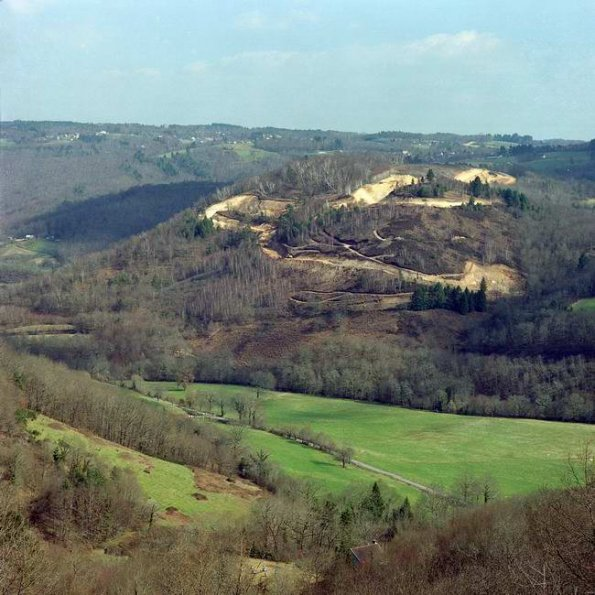
\includegraphics[width=\textwidth]{images/intro/opp_01}
	\end{subfigure}
	~
	 \begin{subfigure}[t]{0.3\textwidth}	
			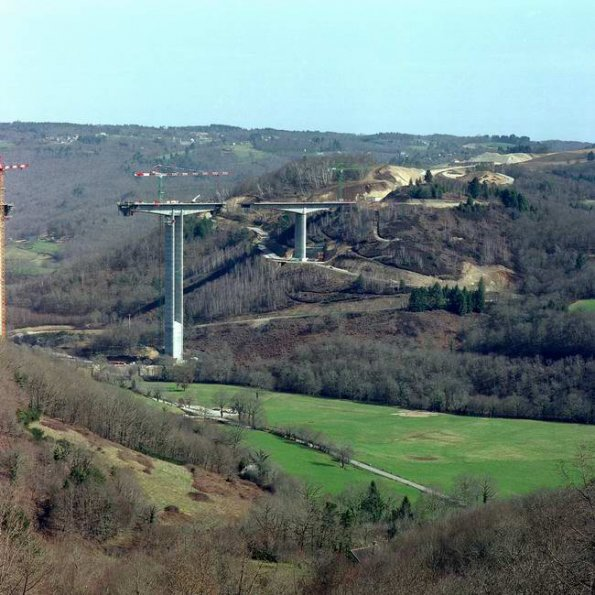
\includegraphics[width=\textwidth]{images/intro/opp_02}
	\end{subfigure}
	~
	 \begin{subfigure}[t]{0.3\textwidth}	
			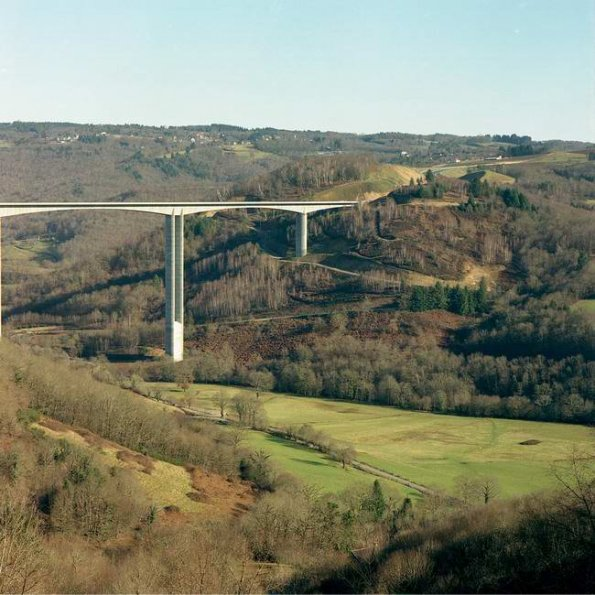
\includegraphics[width=\textwidth]{images/intro/opp_03}
	\end{subfigure}
	\caption{Photographie\modif{s} extraite\modif{s} de l'observatoire photographique du paysage mis en place lors \modif{de la construction} de l'autoroute A89.}
	\label{fig:intro:oppex}
\end{figure}

L'examen de ces fonds par des experts (géographes, personnes en charge de l'aménagement du territoire, etc.) permet d'analyser l'évolution d'un paysage lors d'un événement spécifique (construction d'un pont, chantier d'une \modif{autoroute}) ou d'étudier la dynamique de zones particulières (les territoires \modif{périurbains} par exemple). Leur mise à disposition pour le grand public participe à la valorisation du patrimoine \modif{paysager} et offre un outil aux citoyens pour s'impliquer davantage dans les actions publiques pouvant influencer \modif{leur} cadre de vie. 


La création, l'enrichissement et la consultation des données d'un observatoire photographique du paysage fait intervenir de nombreux outils informatiques. A minima, un observatoire photographique du paysage donne lieu à la mise en place d'un site web, par le biais duquel l'ensemble des citoyens peuvent accéder aux différentes séries de \modif{photographies}. La mise en place de traitements plus fins, capables d'extraire des informations pertinentes de ce catalogue d'images offrent de nombreux défis dans le domaine de la vision par ordinateur.

\section{Vision par ordinateur}
Olivier Faugeras \cite{faugeras1993three} définit la vision par ordinateur comme la discipline se focalisant  sur les quatre problèmes \modif{suivants} :

\begin{itemize}
\item quelles informations peuvent être extraites à partir des données enregistrées par un capteur visuel (caméra, appareil photographique, etc.)\modif{?}
\item comment ces informations sont-elle extraites ?
\item comment doivent-elles être représentées ? 
\item à quel point peuvent-elles être utilisées par un système robotique pour réaliser une tâche donnée ? 
\end{itemize}

Actuellement les applications \modif{de} ce domaine débordent largement de la robotique et la vision par ordinateur peut être vue comme la construction de modèles algorithmiques possédant des propriétés semblables à celle de la vision humaine. Ainsi, à l'aide \modif{d'un ensemble} de connaissances \textit{a priori}, l'enjeu consiste à fournir une interprétation de l'information contenu dans \modif{une ou plusieurs images}. Concrètement, il s'agit d'extraire des primitives visuelles de l'image, de proposer une représentation des connaissances et de mettre l'une et l'autre en correspondance afin de fournir une interprétation fiable  et rapide de la scène. 

Les problèmes classiques en vision par ordinateur sont, par exemple, les procédés de contrôle de pièce dans la robotique industrielle, la navigation pour les véhicules autonome\modif{s}, la détection d’événements, la modélisation 3D d'objets ou d'environnement\modif{s}, la reconnaissance d'objets, etc.


\section{Application dans le cadre des observatoires photographiques du paysage}

Dans le contexte des observatoires du paysage, \modif{le capteur visuel peut être un smartphone, un appareil photographique grand public ou un appareil photographique professionnel}. Les données obtenues sont  des photographies \modif{couleur de grande taille}. \modif{Ces images sont généralement de bonne qualité : elles sont peu bruitées et les objets qu'elles contiennent sont nets}. La figure \ref{fig:intro:oppex} montre \modif{trois} images extraites d'une même série.

Nos travaux concernent l'identification et la localisation des objets présents dans ces photographies. Nous souhaitons attribuer à chaque pixel un label indiquant \modif{la catégorie d'objet à laquelle} il appartient (ciel, herbe, route, etc.). Parce qu'ils permettent d'extraire les régions correspondant aux éléments d'une image et de leur attribuer une signification, les algorithmes visant à réaliser de tels traitements appartiennent au domaine de \emph{\modif{la} segmentation sémantique}. Les méthodes produites au sein de cette thématique de recherche peuvent être entièrement automatiques ou bien semi-automatique\modif{s}. 

Nous avons choisi de nous intéresser aux méthodes semi-automatique\modif{s}, dans la perspective de créer un outil permettant d'enrichir les données d'un observatoire photographique du paysage. \modif{Cet outil} intervient au sein d'une application plus complexe, capable de guider un utilisateur vers le point à re-photographier le plus proche puis de l'aider à reprendre une photographie à l'identique. Avant d'être envoyé à un serveur stockant les séries de photographies, cette dernière peut alors être segmentée de manière à ce que les éléments importants qu'elle contient soit documentés et localisés précisément dans l'image. 

Formulé différemment, nous cherchons un moyen  efficace de sélectionner chacun des objets visibles et de lui attribuer un label correspondant à des catégories sémantiques propres à l'observatoire. Ce type de logiciel est appelé \emph{outil de segmentation interactive}.


\section{Segmentation interactive }

Une méthode de segmentation interactive est un outil informatique capable de sélectionner un ou plusieurs objets au sein d'une image \modif{à partir d'indications données par un utilisateur}. Le domaine d'application le plus courant \modif{de ce type d'algorithme} est celui des logiciels de \modif{manipulation} d'images, dont les deux plus connus sont sans doute Gimp \footnote{\url{http://gimp.org}} et Photoshop \footnote{\url{http://www.photoshop.com}}. 

\begin{emodif}
Ce type d'algorithme se situe au croisement de deux thématiques : celle de la vision par ordinateur et celle de l'étude des interactions entre l'homme et la machine. 

Du point de vue de la vision par ordinateur, un accent particulier sera mis sur la formulation du problème de la segmentation interactive et sur les hypothèses qu'elle émet vis-à-vis du résultat recherché. Par exemple, certaines méthodes de segmentation interactive sont conçues pour extraire un unique objet du fond. Au contraire, d'autres algorithmes s'intéressent à la sélection simultanée de plusieurs objets, ce qui implique une augmentation significative de l'espace des solutions possibles. D'autres problématiques interviennent également de manière récurrente :  
\begin{itemize}
\item quelles primitives visuelles utiliser ? Par exemple, faut-il travailler directement au niveau du pixel ou rechercher des primitives visuelles plus complexes, telles que des groupes de pixels ? 
\item les indications données par l'utilisateur doivent-elles être considérées comme fiables ou faut-il envisager qu'elles contiennent des erreurs ? 
\item quel est le coût pour extraire un type d'information par rapport à son bénéfice dans la recherche d'un résultat ? Par exemple, si l'accès à la couleur d'un pixel est immédiat, analyser la texture présente dans son voisinage est une opération plus complexe, dont nous pouvons interroger la pertinence. 
\item est-il possible de trouver une solution exacte au problème posé ou faut-il se contenter d'une approximation ?
\item quelles approches permettent une recherche rapide de cette solution, qu'elle soit exacte ou approchée ?
\end{itemize}

L'étude des interactions entre l'utilisateur et le programme mettra l'accent sur l'ergonomie de la méthode de segmentation interactive, se demandant par exemple :
\begin{itemize}
\item quelles modalités permettent à l'utilisateur de donner les indications nécessaires à la méthode ? 
\item pour une  modalité donnée, quel est son degré de pénibilité ?
\item l'impact de ces indications sur le résultat obtenu est-il facilement prévisible par l'utilisateur ? 
\item est-il facile d'apprendre à se servir de la méthode proposée ?
\item le temps nécessaire à la méthode pour obtenir un résultat à partir des indications en permet-il une utilisation fluide ? 
\end{itemize}


\end{emodif}

 
\section{Problématique}

Le problème que nous cherchons à résoudre est le suivant : soit une photographie couleur et un ensemble de pixels attribués à différentes \modif{catégories} par un utilisateur ; comment associer de manière fiable et efficace chaque pixel de l'image à l'une des \modif{catégories demandées} par l'utilisateur et ce, de façon à ce que la segmentation sémantique produite soit cohérente tant vis-à-vis du \modif{contenu de l'image} que des indications fournies par l'utilisateur ? 


Nous ne souhaitons pas nous limiter aux seules photographies des observatoires du paysage et cherchons à concevoir un outil de segmentation interactive qui \modif{pourrait constituer} une amélioration intéressante \modif{par rapport à ceux} utilisés actuellement dans les logiciels de manipulation d'images. Ainsi, nous n'avons aucune connaissance \textit{a priori} sur le contenu des photographies ni sur les objets que l'utilisateur souhaitera sélectionner. En d'autre\modif{s} terme\modif{s}, seules les indications données par l'utilisateur permettent d'apprendre les \modif{caractéristiques des catégories d'objets}. Cet apprentissage est propre à chaque photographie et doit être recommencé pour chaque nouvelle image. 

\begin{emodif}
Nous ne nous donnons pas de limite sur le nombre d'objets à sélectionner et nous considérons que ce dernier varie d'une image à l'autre. Nous nous intéressons à la conception d'un algorithme itératif, où l'utilisateur peut corriger de manière intuitive les erreurs contenues dans le résultat obtenu, afin de converger rapidement vers la sélection qu'il désire. Nous supposons également que les indications données par l'utilisateur sont majoritairement fiables. 
\end{emodif}

Enfin, l'une des contraintes importantes de nos travaux concerne \modif{la rapidité} de la méthode que nous proposons. Dans le contexte des observatoires photographiques du paysage comme dans celui d'un logiciel de manipulation d'images, les photographies à traiter contiennent plusieurs millions de pixels. Le caractère interactif des algorithmes de segmentation interactive impose qu'un résultat soit fournit rapidement à l'utilisateur.  Notre choix des primitives visuelles et de la manière dont nous les utilisons doit garantir une faible complexité algorithmique.


\section{Organisation du mémoire}

Ce mémoire comprend sept chapitres.

\subsubsection*{\modif{Chapitre 1 -- Introduction --}} 
\modif{Nous présentons les motivations à l'origine des travaux décrits dans ce mémoire.}

\subsubsection*{\modif{Chapitre 2 -- Segmentation interactive --}} 
Nous présentons le domaine de la segmentation interactive et nous proposons une catégorisation des méthodes appartenant à cette \modif{thématique} : les méthodes de binarisation interactive par recherche des contours, les méthodes de binarisation interactive par recherche des régions \modif{et} les méthodes \modif{ de segmentation interactive multiclasse}. Pour chaque catégorie\modif{,} nous présentons quelques algorithmes de référence. 

\subsubsection*{\modif{Chapitre 3 -- Algorithme de segmentation interactive Superpixel $\alpha$-Fusion --}}
Nous proposons une nouvelle méthode de segmentation interactive \modif{multiclasse} $S \alpha F$, de l'anglais \og \emph{Superpixel $\alpha$-Fusion}\fg. Nous commençons par \modif{formuler} le problème de la segmentation interactive comme la minimisation d'une \modif{fonction de coût}. Cette fonction pouvant être factorisée, nous nous ramènerons à un problème d'optimisation dans un graphe de \modif{facteurs}. Un graphe de \modif{facteurs} est un graphe biparti où les sommets sont séparés en deux ensembles : les variables et les facteurs. \modif{Dans notre cas, les variables correspondent à de petits groupes connexes et homogènes de pixels : les superpixels}. Les facteurs correspondent aux sous-fonctions. Nous verrons comment les valeurs numériques de ces sous-fonctions peuvent être obtenues à l'aide d'une méthode de classification. 

\subsection*{\modif{Chapitre 4 --  Évaluation des méthodes de sur-segmentation --}}
Produire une sur-segmentation d'une image consiste à trouver une partition de ses pixels en petits ensembles connexes (les superpixels), dont la taille est nettement inférieure à celle des \modif{objets}. Pour la méthode que nous proposons, l'obtention d'une sur-segmentation est une étape clé. Nous avons donc réalisé une évaluation rigoureuse des algorithmes de sur-segmentation. Si la principale motivation de ce travail reste de sélectionner l'algorithme le plus approprié pour la méthode $S \alpha F$, les conclusions que permettent de tirer cette évaluation dépassent largement le cadre de la segmentation interactive.

\subsection*{\modif{Chapitre 5 -- Évaluation de l'algorithme $S \alpha F$ --}}

Ce chapitre concerne l'évaluation de $S \alpha F$. Nous comparons ses performances à celles des algorithmes de l'état de l'art \modif{décrits} dans le chapitre 2. Puis nous nous intéressons aux propriétés de \modif{$S \alpha F$}, notamment celles concernant son ergonomie. Nous concluons par deux applications de $S \alpha F$ : comme greffon pour le logiciel Gimp et comme outil d'annotation pour l'enrichissement d'un observatoire photographique du paysage.

\subsection*{\modif{Chapitre 6 -- Sur-segmentation adaptative par fusion de superpixels --} }

Nous terminons ce \modif{mémoire} par la proposition d'un nouvel algorithme de sur-segmentation, $ASARI$, de l'anglais \og \emph{\modif{Adaptive Superpixel Algorithm with Rich Information}}\fg . Ce dernier permet d'obtenir \modif{une} précision supérieure ou égale à celles des méthodes de l'état de l'art, avec un nombre \modif{inférieur} de superpixel\modif{s}. Par ailleurs\modif{,} les superpixels produits sont homogènes au sens de \modif{la} couleur et au sens de la texture. 

L'intégration de cet algorithme au sein de $S \alpha F$  constitue une perspective intéressante pour améliorer ses résultats. Elle requiert cependant :
\begin{itemize}
\item d'optimiser l'implémentation d'$ASARI$, les temps d'exécution de ce dernier étant encore trop important\modif{s} pour l'intégrer de manière bénéfique dans une méthode de segmentation interactive \modif{;} 
\item de réaliser des tests approfondis. L'une des particularités des superpixels produits par $ASARI$ étant d'intégrer une information de texture, au delà d'une simple évaluation montrant qu'$ASARI$ permet d'améliorer les performances de $S \alpha F$, il convient de vérifier si cette information de texture peut ou non avoir une influence positive sur la qualité des segmentations réalisées par $S \alpha F$.
\end{itemize}

Ces travaux restent à mener.


\subsubsection*{\modif{Chapitre 7 -- Conclusion -- }} 

\modif{Nous terminons par un résumé des contributions présentées et par quelques prolongements possibles de nos travaux.}

\glsresetall
\chapter{Segmentation interactive }

\section{Introduction}

Ce chapitre traite de la segmentation interactive. Comme son nom l'indique, ce domaine de recherche est rattaché à celui de la segmentation. Il comprend un ensemble de méthodes semi-automatiques, où l'utilisateur fournit les indications nécessaires à l'obtention d'un résultat. 

Afin de bien en comprendre les enjeux, nous commencerons par quelques rappels sur la \modif{segmentation qui} nous permettront de définir la segmentation interactive. Nous nous intéresserons ensuite aux différentes pistes explorées jusqu'à présent et nous présenterons quelques algorithmes clés de l'état de l'art. 


\subsection{Segmentation}

La segmentation est une étape \modif{clé pour} un grand nombre de \modif{méthodes} d'analyse d'images. Son but consiste à produire une partition des pixels de l'image en composantes connexes, selon des critères prédéfinis (homogénéité en \modif{termes} de couleurs, de texture, etc.). Ces composantes connexes sont nommées régions et correspondent à des objets ou à des parties d'objets, formant un pavage de l'image en primitives visuelles de haut niveau. La figure \ref{fig:sota:seg-ex} contient un exemple de segmentation. Les pixels de l'image originale (figure \ref{fig:sota:seg-ex}a) sont groupés en une dizaine de régions (figure \ref{fig:sota:seg-ex}b). La figure \ref{fig:sota:seg-ex}c représente les contours de ces régions, \modif{où apparaissent} en blanc les pixels ayant un de leurs voisins qui appartient à une autre région.

\begin{figure}[htb]
\centering
	 \begin{subfigure}[t]{0.3\textwidth}	
			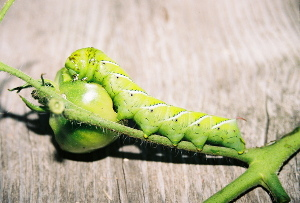
\includegraphics[width=\textwidth]{images/etat-de-l-art/img-065-im}
		 \caption{Image originale. }
	\end{subfigure}
	~
	 \begin{subfigure}[t]{0.3\textwidth}	
			
\includegraphics[width=\textwidth]{images/etat-de-l-art/img-065-seg}
		 \caption{Segmentation \modif{de} cette image : une couleur par \modif{région.}}
	\end{subfigure}
	~
	 \begin{subfigure}[t]{0.3\textwidth}	
			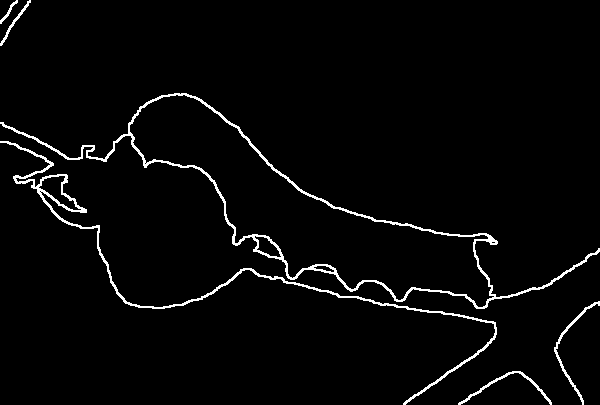
\includegraphics[width=\textwidth]{images/etat-de-l-art/img-065-bdr}
		 \caption{Contours des régions de cette segmentation.}
	\end{subfigure}
	\caption{Exemple \modif{de} segmentation.}
	\label{fig:sota:seg-ex}
\end{figure}


Trois \modif{hypothèses} guident les travaux menés en segmentation :
\begin{itemize}
\item l'homogénéité à l'intérieur de chaque région en \modif{termes} de couleur \modif{ou} de texture doit être maximisée ;
\item les similitudes entre les différentes régions doivent être minimisées ;
\item les pixels voisins appartenant à des régions différentes doivent être aussi dissemblables que possible.
\end{itemize} 



\subsection{Segmentation sémantique}

Tandis que la segmentation se contente de produire un pavage de l'image en régions, la segmentation sémantique réalise une partition des pixels en ensembles qui correspondent \modif{à des catégories d'objets}. Comme un même objet peut correspondre à plusieurs régions \modif{ou plusieurs objets de la même catégorie être présents dans l'image}, les ensembles ne sont pas nécessairement des composantes connexes. Si le problème de la segmentation peut être vu comme la recherche des frontières des objets présents dans une photographie, celui de la segmentation sémantique consiste à  localiser et identifier les \modif{objets qui la composent c'est-à-dire comme la résolution d'un problème de classification, avec une classe par catégorie d’objets}. La figure \ref{fig:sota:seg-sem-ex}b contient \modif{une} segmentation sémantique associée à la figure \ref{fig:sota:seg-sem-ex}a. Les pixels se répartissent en trois ensembles : le premier correspondant à une table en bois (en jaune), le second à la chenille (en rose) et le troisième à la branche de tomate (en bleu).

\begin{figure}[htb]
\centering
	 \begin{subfigure}[t]{0.3\textwidth}	
			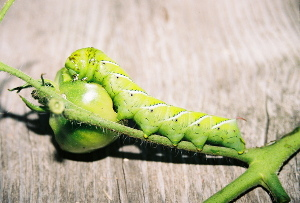
\includegraphics[width=\textwidth]{images/etat-de-l-art/img-065-im}
		 \caption{Image originale. }
	\end{subfigure}
	~
	 \begin{subfigure}[t]{0.3\textwidth}	
			
\includegraphics[width=\textwidth]{images/etat-de-l-art/img-065-seg-semantique}
		 \caption{Segmentation sémantique \modif{de} cette image. Trois classes sont \modif{identifiées} : le bois (en jaune), la chenille (en rose) et la tomate (en bleu).}
	\end{subfigure}
	\caption{\modif{Exemple de} segmentation sémantique.}
	\label{fig:sota:seg-sem-ex}
\end{figure}


L'utilisation des réseaux de neurones convolutifs (CNN, de l'anglais \og \emph{Convolutional Neural Networks} \fg) \modif{et de l'apprentissage profond ont} conduit à des \modif{avancées} significatives dans le domaine la \modif{segmentation} sémantique  \cite{fourure2017multi,garcia2017review,long2015fully}. Toutefois, malgré la qualité impressionnante des \modif{résultats} obtenus,  ce type de méthode ne peut être guidée que lors de l'étape d'apprentissage \cite{lin2016scribblesup}. 

L'un des inconvénients les plus évidents de cette contrainte réside dans le fait que lorsque la méthode produit une segmentation erronée, il n'est pas possible de \modif{la} corriger sans recommencer l'apprentissage du CNN, lequel nécessite \modif{une quantité de données d'apprentissage importante et} de nombreuses heures de calculs. \modif{Par ailleurs, le CNN est entraîné à reconnaître un nombre fini de classes, définies lors de l'apprentissage. Pour introduire une nouvelle classe, il faut recommencer l'étape d'apprentissage.} 

La résolution de ces deux problèmes \modif{peut passer} par la recherche de méthodes semi-au\-to\-ma\-ti\-ques, intégrant de manière plus souple l'intervention d'un utilisateur. Elle correspond au domaine de la segmentation \modif{interactive}. 

\subsection{Segmentation interactive }

Le principe de la segmentation interactive consiste guider la recherche d'une segmentation particulière en intégrant quelques indications fournies par un utilisateur. Le fonctionnement général d'une méthode de segmentation interactive est illustré par la figure \ref{fig:sota:segInt}. Une photographie est donnée à l'utilisateur qui décide des \modif{entités} qu'il souhaite \modif{sélectionner}. \modif{Notons que l'utilisateur peut choisir ou non de produire une segmentation sémantique. Dans certains cas, il souhaitera sélectionner ensemble tous les objets d'une même catégorie (par exemples, tous les arbres). Dans d'autres, il pourra ne vouloir sélectionner qu'un seul objet, appartenant à une catégorie représentée plusieurs fois dans l'image (par exemple, un arbre spécifique).}

Les indications \modif{que l'utilisateur} donne permettent à la méthode de produire un premier résultat. Le plus souvent ce dernier ne correspond pas exactement aux attentes de l'utilisateur, qui vient ajouter ou supprimer des indications, déclenchant la recherche d'une deuxième segmentation. Ce processus est répété jusqu'à satisfaction des objectifs de l'utilisateur.

\begin{figure}[htb]
	\centering
		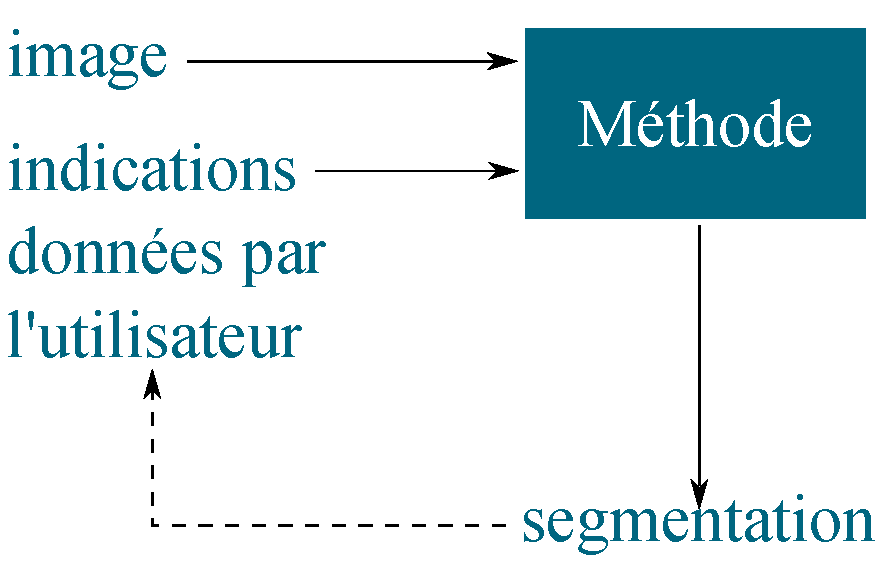
\includegraphics[width=0.45\textwidth]{images/etat-de-l-art/segInt}
		\caption{Processus\modif{, pouvant être itératif}, d'utilisation d'une méthode de segmentation interactive.}
		 \label{fig:sota:segInt}
\end{figure}


\modif{Soit $I$ une image}.  Soit \modif{$\mathbb{P}=\lbrace p_{1}, \cdots, p_{N_{I}} \rbrace$} l'ensemble des $N_{I}$ pixels de $I$. Soit \modif{$\Lambda=\lbrace \lambda_{1},\cdots,\lambda_{N_{\Lambda}} \rbrace$} un ensemble de $N_{\Lambda}$ labels indexant chaque classe, avec une classe par \modif{entité} \modif{que l'utilisateur souhaite sélectionner}.  Les indications données par l'utilisateur prennent la forme d'un ensemble  $G= \lbrace g_{1}, \cdots, g_{N_{G}} \rbrace$ dont chaque élément $g_{i}$ est un couple de valeurs $(p_{i},\lambda_{j})$, tel que  \modif{$p_{i} \in \mathbb{P} $} et \modif{$\lambda_{i} \in \Lambda$}. Réaliser une segmentation interactive de $I$ consiste à associer à chaque élément de \modif{$\mathbb{P}$} un unique élément de \modif{$\Lambda$}, en garantissant le maximum de cohérence :
\begin{itemize}
\item avec le contenu de l'image ;
\item entre les pixels attribués à une classe et les indications données par l'utilisateur.
\end{itemize}

La communication de l'utilisateur vers la méthode s'effectue par le biais des indications (l'ensemble $G$). \modif{Certaines méthodes de segmentation interactive considèrent ces indications comme parfaitement fiables \cite{boykov2001interactive,salembier2000binary}, d'autres comme pouvant contenir des erreurs \cite{ Changjae2017Robust,muller2016robust}}. La communication de la méthode vers l'utilisateur \modif{est assurée} par l'affichage d'une segmentation de l'image.

Ces deux caractéristiques imposent, entre autres : 
\begin{itemize}
\item que l'impact d'une indication sur le résultat soit facilement prévisible par l'utilisateur, afin qu'il puisse guider efficacement la méthode ;
\item que les modalités d'\modif{interaction} permettant d'ajouter ou de retirer une indication soient faciles d'utilisation ;
\item que le temps nécessaire pour obtenir une segmentation à partir d'une image et d'un ensemble d'indications demeure suffisamment court pour permettre une interaction fluide (généralement nous considérerons que cette durée ne peut excéder quelques secondes).
\end{itemize}

Il s'avère intéressant de mettre ce dernier point en relation avec le contexte d'application des méthodes de segmentation interactive. Actuellement, ces dernières sont employées afin de sélectionner des objets au sein d'une photographie pour leur appliquer des traitements particuliers ou pour les intégrer au sein d'un collage, dans le domaine artistique ou dans celui du design. Les images à traiter comportent souvent plusieurs millions de pixels, ce qui soulève la question du passage à l'échelle des algorithmes de segmentation interactive. Enfin, si actuellement la majorité de ces méthodes sont implémentées pour des ordinateurs, le remplacement progressif de ce type de machine par des smartphones auprès du grand \modif{public} requiert d'envisager des algorithmes capables de passer à l'échelle malgré des contraintes matérielles \modif{importantes} (taille de la mémoire vive, capacité du processeur, puissance de la carte graphique, etc.).


\subsection{Catégorisation}

\modif{Durant ces} deux dernières décennies, le domaine de la segmentation interactive s'est enrichi de nombreux algorithmes.  Dans ce mémoire, nous proposons de les classer en trois catégories :
\begin{itemize}
\item \textbf{Binarisation interactive par recherche des contours - } Ces algorithmes déterminent pour chaque pixel s'il appartient ou non au contour de l'objet d'intérêt. Il s'agit donc d'un problème de classification à deux classes,  $\lambda_{C}$ pour les pixels du contour, $\lambda_{\neg C}$ pour les autres.  L'utilisateur indique quelques pixels de la classe $\lambda_{C}$. 
\item \textbf{Binarisation interactive par recherche des régions - } Ces algorithmes groupent les pixels de manière à obtenir deux ensembles homogènes. Ces ensembles \modif{correspondent} à une ou plusieurs composantes connexes. Il s'agit là aussi d'un problème de classification à deux classes avec, d'une part, les pixels de l'objet principal ($\lambda_{O}$) et, d'autre part, ceux du fond  ($\lambda_{F}$). L'utilisateur attribue quelques pixels à chacune des deux classes. 
\item \textbf{Segmentation interactive \modif{multiclasse} - } Ces algorithmes correspondent à une généralisation de la catégorie précédente, où le nombre de classes n'est plus limité à deux. 
\end{itemize}



\section{\modif{Lexique et notations}}

\subsection{\modif{Lexique}}
Par la suite, nous utiliserons \modif{les termes} :

\begin{itemize}
\item \textbf{germe}, pour désigner le pixel attribué à une classe par l'utilisateur (un germe correspond à une indication)  ;
\item \textbf{classe},  pour désigner  une \modif{entité (un objet ou une catégorie d'objets)} à laquelle certains pixels seront assignés à l'issue du processus de segmentation;
\item \textbf{segmentation}, pour désigner le résultat produit par une méthode de segmentation interactive à chaque itération ;
\item \textbf{région}, pour désigner un ensemble de pixels connexes appartenant à la même classe.
\end{itemize}

\subsection{Notations}

Soit $I$ une image.
\begin{itemize}
\item \textbf{L'ensemble} $\mathbb{P}= \lbrace p_{1}, \cdots, p_{N_{I}} \rbrace$ contient les pixels de $I$.
\item \textbf{La fonction}  $\nei(p)$ donne l'ensemble des pixels voisins du pixel $p$.  La figure \ref{fig:sota:vois} décrit les trois principaux systèmes de voisinage : les quatre voisins (nord, est, sud, ouest), les huit voisins (nord, nord-est, est, sud-est, sud, sud-ouest, ouest, nord-ouest) et le voisinage circulaire qui comprend les $N_{voi}$ voisins répartis \modif{régulièrement} sur le cercle \modif{de rayon $r$} ayant pour centre le pixel $p$. Dans ce dernier cas, le niveau de gris d'un voisin est obtenu par interpolation des niveaux de gris environnants.
\begin{figure}[htb]
	\centering
	 \begin{subfigure}[t]{0.2\textwidth}	
			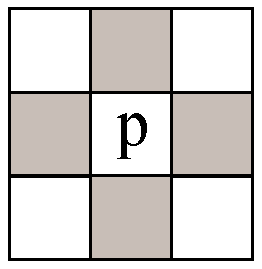
\includegraphics[width=\textwidth]{images/etat-de-l-art/4V}
		 \caption{4-voisinage.}
			\label{fig:sota:vois4}
	\end{subfigure}
	~
	 \begin{subfigure}[t]{0.2\textwidth}	
			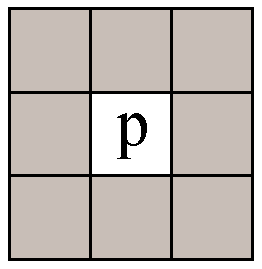
\includegraphics[width=\textwidth]{images/etat-de-l-art/8V}
		 \caption{8-voisinage.}
			\label{fig:sota::vois8}
	\end{subfigure}
	~
	 \begin{subfigure}[t]{0.2\textwidth}	
			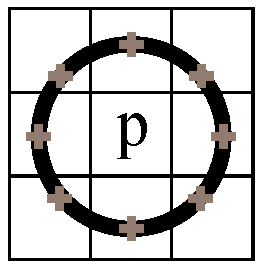
\includegraphics[width=\textwidth]{images/etat-de-l-art/CV}
		 \caption{Voisinage circulaire.}
			\label{fig:sota::voisC}
			
	\end{subfigure}
	\caption{Les principaux systèmes de voisinage pour un pixel.}
	\label{fig:sota:vois}
\end{figure}

\item \textbf{Le graphe} $\mathcal{G}=\ <V,E>$ est une représentation de $I$, où $V=\lbrace v_{1},\cdots, v_{N_{I}} \rbrace$ est un ensemble de $N_{I}$ sommets correspondant aux pixels de $I$ et $E$ un ensemble d'arêtes reliant les sommets $v_{i}$ et $v_{j}$ si et seulement s'ils correspondent à des pixels voisins. Un exemple d'un tel graphe est donné sur la figure \ref{fig:sota:im_to_g}.

\item \textbf{L'arête} $e_{i,j}$ relie les sommets $v_{i}$ et $v_{j}$, correspondant respectivement aux   \modif{$i\ieme$}  et  \modif{$j\ieme$}  pixels. 
\item \textbf{Le poids }$w_{i,j}$ est le réel associé à l'arête $e_{i,j}$.
\item \textbf{Une segmentation } \modif{$S = \lbrace s_{1}, \cdots, s_{N_{S}} \rbrace$} de $I$ consiste en  une partition de $\mathcal{G}$ en $N_{S}$ \modif{composantes connexes}.
\item \textbf{L'ensemble} \modif{$ \Lambda =\lbrace \lambda_{1},\cdots,\lambda_{N_{\Lambda}}  \rbrace $} contient les labels associés aux $N_{\Lambda}$ classes.
\item \textbf{Les germes donnés par l'utilisateur} sont représentés sous la forme d'un ensemble $G= \lbrace g_{1}, \cdots, g_{N_{G}} \rbrace$, où chaque élément $g_{i}$ est un couple de valeurs $(p_{i},\lambda_{j})$, tel que \modif{$p_{i} \in \mathbb{P}$}  \modif{et $\lambda_{i} \in \Lambda$}.
\item \textbf{La fonction de coût} $ \mathcal{F}(I,S,G)$ permet d'évaluer la pertinence d'une segmentation $S$ de $I$, par rapport aux caractéristiques intrinsèques de $I$ et aux germes $G$.  
\end{itemize}


\begin{figure}[htb]
	\centering
	 \begin{subfigure}[t]{0.3\textwidth}	
			
\includegraphics[width=\textwidth]{images/etat-de-l-art/grahIm}
		 \caption{Réprésentation d'une image couleur de $4 \times 4$ pixels.}
			\label{fig:sota:img_graph1}
	\end{subfigure}
	~
	 \begin{subfigure}[t]{0.3\textwidth}	
			
\includegraphics[width=\textwidth]{images/etat-de-l-art/grahIm2}
		 \caption{Graphe construit à partir de l'image. Nous considérons ici que les pixels
		 sont voisins au sens du 4-voisinage. L'épaisseur des arêtes est proportionnelle au degré de similarité entre les pixels.}
			\label{fig:sota::img_graph1}
	\end{subfigure}
	\caption{Représentation d'une image par un graphe.}
	\label{fig:sota:im_to_g}
\end{figure}

\section{Méthodes de binarisation interactive par recherche des contours}

\subsection{Formulation du problème}

Les méthodes de binarisation interactive par recherche des contours séparent un objet du fond en retrouvant les pixels correspondant à son contour. Il s'agit d'un problème de classification à deux classes,  $\lambda_{C}$ si le pixel appartient au contour,  $\lambda_{\neg C}$ sinon. Les germes sont quelques uns des pixels \modif{du contour}. L'ensemble $G$ correspond \modif{donc} à des pixels de label $\lambda_{C}$. 

Soit \modif{$\mathbb{P}_{C}$}, l'ensemble des pixels de label $\lambda_{C}$ \modif{dans le résultat donné par la méthode}. Cet ensemble doit respecter les propriétés suivantes :
\begin{itemize}
\item il doit contenir l'ensemble des pixels de $G$ ;
\item il doit avoir une forte probabilité d'appartenir aux contours de $I$ ;
\item il doit former une courbe fermée (voir la figure \ref{fig:sota:courbeSimp}) ;
\item cette courbe doit être aussi simple que possible et notamment éviter de se croiser (voir la figure \ref{fig:sota:courbeX}) ou de se chevaucher (voir la figure \ref{fig:sota:courbeChe}).
\end{itemize} 

\modif{Il n'existe pas à ce jour de méthode de binarisation interactive par recherche des contours résolvant} des problèmes multiclasses : le chemin formé par les pixels de label  $\lambda_{C}$ étant fermé, la segmentation $S$ obtenue \modif{contient uniquement deux régions}, l'une correspondant à l'objet à extraire $S_{O}$ et l'autre au fond $S_{F}$.  

\begin{figure}[htb]
	\centering
	 \begin{subfigure}[t]{0.25\textwidth}	
			
\includegraphics[width=\textwidth]{images/etat-de-l-art/courbe3}
		 \caption{Courbe simple.}
			\label{fig:sota:courbeSimp}
	\end{subfigure}
	~
	 \begin{subfigure}[t]{0.25\textwidth}	
			
\includegraphics[width=\textwidth]{images/etat-de-l-art/courbe2}
		 \caption{Courbe se croisant.}
			\label{fig:sota:courbeX}
	\end{subfigure}
	~
	 \begin{subfigure}[t]{0.25\textwidth}	
			
\includegraphics[width=\textwidth]{images/etat-de-l-art/courbe1}
		 \caption{Courbe se chevauchant. }
			\label{fig:sota:courbeChe}
	\end{subfigure}
	\caption{Quelques types de courbes.}
	\label{fig:sota:courbes}
\end{figure}

\subsection{Interaction avec l'utilisateur}

La figure \ref{fig:sota_boundary_based_ihm} illustre le type \modif{d'indications généralement associé} aux méthodes de binarisation par recherche des contours. Les germes donnés par l'utilisateur sont représentés par de petits disques clairs. Le contour trouvé par la méthode est affiché sur la forme de traits blancs bordés de noir. Lorsque celui-ci s'avère erroné, l'utilisateur peut ajouter, déplacer ou supprimer certains germes. 

\begin{figure}[htb]
	\centering
			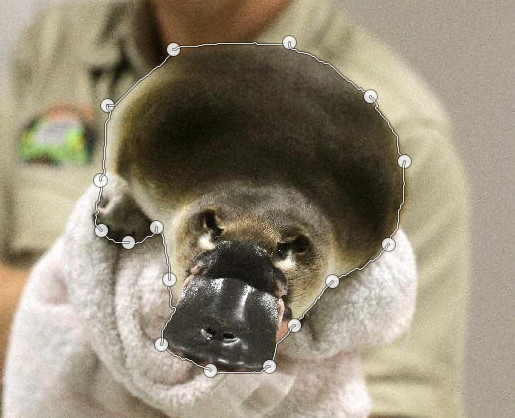
\includegraphics[height=0.35\textheight]{images/etat-de-l-art/boundary-based-method2}
		 \caption{Binarisation interactive par recherche des contours : exemple d'interaction avec l'utilisateur. \modif{ Les germes donnés par l'utilisateur apparaissent sous la forme de disques blancs. Le contour trouvé par la méthode est indiqué par un trait blanc bordé de noir.}}
		 \label{fig:sota_boundary_based_ihm}
\end{figure}

Même s'il permet de modifier facilement la forme de la courbe, ce mode d'interaction présente deux désavantages. Tout d'abord, dans des zones où les contours n'apparaissent pas de manière nette (par exemple parce que l'objet est flou ou en raison d'un faible contraste), l'utilisateur peut être contraint de donner de très nombreux germes, ce qui rend rapidement le procédé fastidieux et frustrant. Ensuite, du fait qu'aucune erreur n'est tolérée dans les germes (ces derniers doivent être exactement sur le contour de l'objet), il demande à l'utilisateur de pouvoir les désigner avec précision. Si celle-ci est facilement obtenue à l'aide d'un périphérique tel qu'une souris ou une tablette graphique, elle devient problématique pour du matériel reposant sur un écran tactile, tel que les tablettes ou les smartphones. 

\subsection{Méthode de Mortensen \textit{et al.}}

\modif{Proposé} par Mortensen \textit{et al.}, l'algorithme des ciseaux intelligents \cite{mortensen1995intelligent} formule la détection du contour d'un objet (donc des pixels de label $\lambda_{C}$) comme un problème de recherche du plus court chemin au sein d'un graphe. Chaque arête $e_{i,j} \in E$ est pondérée à l'aide de la \modif{mesure suivante} : \modif{
\begin{equation}
 \mathcal{F} _{sim}(i,j) = \nombre{0,43}f_{1}(j) + \nombre{0,43}f_{2}(j) + \nombre{0,14}f_{3}(i,j) 
\end{equation}}
où
\begin{itemize}
\item la fonction binaire $f_{1}$ correspond à la réponse d'un détecteur de contour par passage à 0 du laplacien ;
\item $f_{2}$ \modif{renvoie une} valeur inversement proportionnelle à celle de la norme du gradient de $I$ ;
\item $f_{3}$ est une fonction de régularisation, favorisant les contours réguliers, en pénalisant les variations brusques de la direction du contour.
\end{itemize}

Soit $I_{Lap}$ le résultat de la convolution d'une image $I$ par le \modif{masque laplacien $K_{Lap}$ : }
\begin{equation}
K_{Lap} = 
\label{eq:sota:laplacien}
\begin{bmatrix}
0 & 1 & 0\\
1 & -4 & 1\\
0 & 1 & 0
\end{bmatrix}\text{.}
\end{equation}

La matrice $I_{Lap}$ correspond à une approximation \modif{du laplacien de $I$} \modif{dont les passages à 0 coïncident théoriquement avec des points de contour dans l'image}. Mortensen \textit{et al.} \modif{détectent  un élément $I_{Lap}(i)$ comme un point de contour} si au moins l'un de ses voisins est de signe différent et si \modif{sa} valeur absolue est inférieure ou égale à la valeur absolue de \modif{chacun de }ses voisins. \modif{Dans ce cas, $f_{1}$} retourne 0, sinon elle renvoie la valeur $1$.

Soit \modif{$I_{x}(j)$} (respectivement \modif{$I_{y}(j)$}) l'approximation discrète de la composante horizontale (respectivement verticale) du vecteur gradient de la fonction niveau de gris de l'image $I$ pour le \modif{$j\ieme$ pixel}. La norme du vecteur gradient de $I$ est obtenue en calculant :
\modif{
\begin{equation}
Grad(j) =\sqrt{\modif{{I_{x}^{2}(j)} + {I_{y}^{2}(j)}}}
\end{equation}
}
et
\modif{
\begin{equation}
f_{2}(j) = \frac{\max(Grad) -Grad(j) }{\max(Grad)}\text{.}
\end{equation}
}

Ainsi, les valeurs retournées par les fonctions $f_{1}$ et $f_{2}$ sont d'autant plus petites que le pixel a une forte probabilité d'appartenir à \modif{l'un} des contours de l'image.

La fonction $f_{3}$, quant à elle, pénalise les changements brusques au niveau de la courbe.

Soit \modif{
\begin{equation}
\overrightarrow{p}_{\perp} =  \frac{\begin{bmatrix}I_y&-I_x\end{bmatrix}^\top}{\|\begin{bmatrix}I_y&-I_x\end{bmatrix}^\top\|}
\end{equation}}
le vecteur unitaire perpendiculaire à la direction du gradient.  \modif{Soit $\overrightarrow{p_{i}}_{\perp}$ ce vecteur pour le $i\ieme$ pixel.} Soit $\overrightarrow{p_{i,j}}$ le vecteur unitaire pointant du \modif{$i\ieme$} pixel vers le  \modif{$j\ieme$} pixel.
Soit le lien bidirectionnel entre les pixels $p{_i}$ et $p_{j}$ : 
\begin{equation}
f_{d}(i,j) =  \begin{cases}
 \overrightarrow{p_{i,j}} &\text{ si }  \overrightarrow{p_{i}}_{\perp} \cdot \overrightarrow{p_{i,j}} \geqslant 0\\
 \overrightarrow{p_{j,i}} &\text{ sinon. }
\end{cases}
\end{equation}
Le terme de lissage de Mortensen \textit{et al.} est calculé de la manière suivante :
\modif{
\begin{equation}
f_{3}(i,j) = \dfrac{2}{3\pi}\bigg(\acos \left(\overrightarrow{p_{i}}_{\perp} \cdot f_{d}(i,j) \right) + \acos(f_{d}(i,j) \cdot \overrightarrow{p_{j}}_{\perp}) \bigg).
\end{equation}
}
Le poids de chaque fonction a été déterminé de manière empirique par Mortensen \textit{et al.} Chaque fois que l'utilisateur indique qu'un pixel appartient au contour de l'objet, le chemin le plus court entre ce pixel et le précédent pixel \modif{sélectionné} est calculé, grâce à l'algorithme de Dijkstra \cite{Dijkstra59anote}. \modif{La courbe est donc construite au fur et à mesure}.

 Mortensen \textit{et al.} proposent une variante de l'algorithme des ciseaux intelligents \cite{mortensen1998interactive}, avec une fonction de similarité plus complexe, dont les poids sont mis à jour à la volée, à partir des caractéristiques des pixels du contour précédemment détectés. Cette variante s'avère pertinente dans le cas où la différence entre l'objet à extraire et le fond est moins marquée que les différences entre certaines composantes au sein de l'une ou l'autre de ces deux classes. La figure \ref{fig:sota_CI_avec_app_ex} montre un exemple de ce cas de figure. L'objet à segmenter est le ventricule gauche, dont le contour est bien moins marqué que celui du cœur. 
 
\begin{figure}[htb]
	\centering
			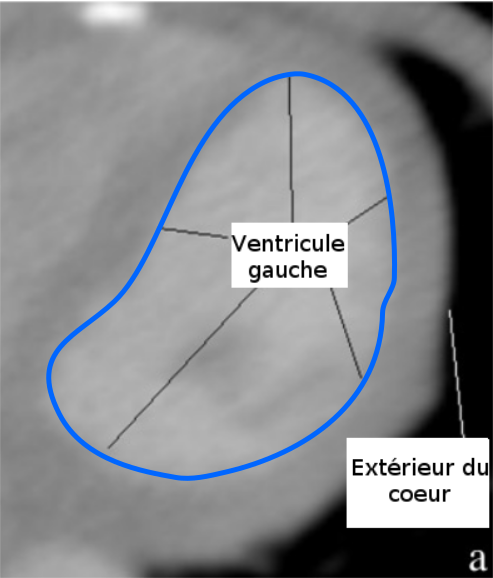
\includegraphics[width=0.25\textwidth]{images/etat-de-l-art/CI_avec_app_ex}
		 \caption{Exemple d'image pour laquelle le contour de l'objet à extraire (en bleu) est moins marqué que le contour entre différents éléments du fond.}
		 \label{fig:sota_CI_avec_app_ex}
\end{figure}

Une autre solution apportée à ce même problème consiste à ne chercher le plus court chemin que dans une partie du graphe. Le plus souvent, \modif{cette} partie correspond à un rectangle englobant les points de départ et d'arrivé du chemin. 

\subsection{Méthode de Mille \textit{et al.}}

L'algorithme par combinaison de chemins géodésiques \cite{mille2015combination} est l'une des plus récentes contributions dans le domaine de la binarisation interactive par recherche des contours. Conçu par Mille \textit{et al.}, il repose sur la recherche d'un chemin fermé  $C$ minimisant
\modif{
\begin{equation}
\mathcal{F}_{CCG}(I,C) = f_{1}(C) + w_{2}f_{2}(I,C) + w_{3}f_{3}(I,C)
\end{equation}
}
avec :
\begin{itemize}
\item \modif{$f_{1}$} une fonction de lissage, dont le résultat est un réel positif qui augmente lorsque certaines portions de la courbe se chevauchent et lorsque la courbe contient des boucles ;
\item \modif{$f_{2}$} une fonction favorisant le passage de la courbe \modif{par} des pixels appartenant aux contours de l'image, en effectuant la somme de l'inverse des normes des vecteurs \modif{gradients} des points de la courbe  ;
\item \modif{$f_{3}$} une fonction qui, en utilisant les coefficients de Bhattacharyya, favorise la production de régions à l'intérieur et à l'extérieur de la \modif{courbe dont} les couleurs correspondent à des distributions statistiques différentes.
\end{itemize} 

À l'instar de l'algorithme des ciseaux intelligents, les germes donnés par l'utilisateur sont ordonnés et forment l'ensemble \modif{$G=\lbrace g_{0}, \cdots, g_{i}, g_{i+1}, \cdots, g_{N_{G}-1} \rbrace$}, où \modif{$g_{i-1}$ est le $i\ieme$ }germe donné par l'utilisateur. Tandis que l'algorithme de Mortensen \textit{et al.} repose sur une approche locale, se contentant de rechercher un chemin optimal entre chaque couple \modif{$(g_{i},g_{((i+1) \mod N_{G})})$}, la méthode de Milles \textit{et al.} \modif{prend en compte} la totalité de la courbe et recherche la \emph{combinaison de chemins} qui minimise $\mathcal{F}_{CCG}$. 


Un parcours exhaustif de l'ensemble de ces combinaisons n'étant pas possible, l'algorithme produit une approximation de la solution en réalisant une \modif{présélection} de chemins probables pour chaque couple \modif{$(g_{i},g_{((i+1) \mod N_{G})})$}. Soit $C_{i}^{*}=\lbrace c_{i}^{1}, \cdots, c_{i}^{m} \rbrace$ l'ensemble de ces chemins probables reliant $g_{i}$ à \modif{$g_{((i+1) \mod N_{G})}$}. \modif{Soit une fonction $f_{D}( c_{i}^{j})$ renvoyant une valeur d'autant moins élevée que le chemin passe par peu de pixels et que ces pixels ont une forte probabilité d'appartenir à un contour, une approximation de la probabilité d'appartenir à un contour étant calculée à partir de la norme du vecteur gradient de la fonction niveau de gris de l'image $I$. Le chemin $c_{i}^{1}$ est le  chemin entre  $g_{i}$ et$g_{((i+1) \mod N_{G})}$, pour lequel la valeur de  $f_{D}$ est minimale}. Le chemin suivant, $c_{i}^{2}$, est obtenu en recherchant à nouveau le plus court chemin, mais sous la contrainte que  $c_{i}^{1}$ et  $c_{i}^{2}$ soient parfaitement distincts, \modif{c'est-à-dire que leurs seuls pixels communs soient $g_{i}$ et $g_{((i+1) \mod N_{G})}$}. 

Même en se limitant à un ensemble discret de chemins possibles entre chaque paire de germes consécutifs, une recherche directe de la combinaison minimisant $\mathcal{F}_{CCG}$ se révèle trop coûteuse en \modif{termes} de temps de calcul. Milles \textit{et al.} \modif{proposent} une heuristique où les chemins entre deux germes sont ordonnés en fonction de leur aire signée, calculée à l'aide du théorème de Green. \modif{Si nous considérons la droite $D_{i}$ passant par deux germes \modif{$g_{i}$ et $g_{((i+1) \mod N_{G})}$} ainsi que la surface $S_{i}^{j}$ délimitée par cette dernière et un chemin donné $c_{i}^{j}$, l'aire signée est calculée en soustrayant l'aire des parties de $S_{i}^{j}$ situées au dessous de $D_{i}$  à l'aire des parties de $S_{i}^{j}$ situées au dessus}.  L'algorithme est initialisé avec les chemins ayant la plus faible aire signée. À chaque itération, une série de combinaisons est produite à partir de la combinaison précédente, en ne changeant qu'un seul chemin. La combinaison minimisant $\mathcal{F}_{CCG}$ est sélectionnée et le processus répété jusqu'à convergence.  

\section{Méthodes de binarisation interactive par recherche des régions}

\subsection{Formulation du problème}
Les algorithmes de binarisation interactive orientés régions cherchent à produire une classification des pixels de l'image en deux catégories : l'objet à extraire (associé au label $\lambda_{O}$) et le fond (associé au label $\lambda_{F}$).  L'utilisateur guide la méthode en associant quelques pixels à chacune des deux classes. Il existe donc une partition de $G$ en deux sous-ensembles, $G_{O}$ pour les germes de label $\lambda_{O}$ et $G_{F}$ pour ceux de label $\lambda_{F}$. 

La segmentation produite par ce type d'algorithme correspond à une partition de l'image en $N_{R}$ régions, $N_{R}$ pouvant être supérieur à deux. Les solutions proposées pour ce problème s'articulent autour de deux grands types d'approches : la minimisation d'une \modif{fonction de coût} et la fusion de régions. 

\subsubsection{Minimisation \modif{d'une fonction de coût}}
Les algorithmes par minimisation \modif{d'une fonction de coût} reposent sur la définition d'une  fonction  de la forme : 
\modif{
\begin{equation}
\mathcal{F}_{C}(I,S,G) = \mathcal{F}_{D}(I,S,G) + \mathcal{F}_{R}(S)
\end{equation}
}
avec :
\begin{itemize}
\item \modif{$\mathcal{F}_{D}$} un terme d'attache aux données, qui évalue l'homogénéité à l'intérieur de chaque région, les dissemblances entre les régions attribuées à des classes différentes et la cohérence entre les \modif{indications données} par l'utilisateur et les pixels attribués à chacune des classes ;
\item \modif{$\mathcal{F}_{R}$} un terme de régularisation qui permet d'éliminer les partitions en de très nombreuses régions \modif{et} les régions avec des contours irréguliers. 
\end{itemize}

Les termes \modif{$\mathcal{F}_{D}$ et $\mathcal{F}_{R}$} sont définis de manière à ce qu'une segmentation optimale vis-à-vis des caractéristiques de l'image et des germes corresponde à une valeur minimale de \modif{$\mathcal{F}_{C}$}. La recherche exacte de ce minimum n'est souvent pas envisageable pour des raisons de temps de calcul et la segmentation obtenue est le résultat d'une approximation.

Les méthodes de Boykov \textit{et al.} \cite{boykov2001interactive}  et \modif{de} Jian \textit{et al.} \cite{jian2016interactive}, \modif{respectivement décrites dans les sections \ref{sec:sota:boykov} et \ref{sec:sota:jian}, constituent} deux exemples de ce type de démarche.
 
\subsubsection{Fusion de régions}

Les algorithmes par fusion de régions produisent une segmentation d'une image en groupant petit à petit les pixels voisins et similaires, de manière à obtenir des ensembles cohérents.

Ce type d'algorithme nécessite une étape d'initialisation où le point de départ de chaque ensemble est donné. Dans le cas de la segmentation interactive, les germes constituent ces embryons de régions qui seront par la suite agrandis. 

Soit $R= \lbrace r_{1}, \cdots, r_{N_{R}} \rbrace $ ces régions initiales, correspondant aux ensembles connexes de germes appartenant à la même classe. À chaque itération de l'algorithme, chacune des $N_{R}$ régions est agrandie en lui ajoutant un ou plusieurs pixels voisins qui :
\begin{itemize}
\item n'ont été attribués à aucune région ;
\item satisfont un critère de similarité avec la région.
\end{itemize}
À chaque fois qu'une région est agrandie, ses caractéristiques sont mises à jour. Lorsque deux régions assignées à la même classe comprennent des pixels adjacents, elles sont également fusionnées. Le processus s'arrête lorsque chaque pixel est attribué à une et une seule région. 

L'algorithme de Salembier \textit{et al.} \cite{salembier2000binary}, \modif{décrit dans la section 
\ref{subsec:sota:salembier}}, constitue un bon exemple d'une méthode de binarisation interactive par fusion de régions. 

\subsection{Interaction avec l'utilisateur}
Le mode d'interaction le plus courant consiste à demander à l'utilisateur de venir tracer des traits de couleur sur chaque région, comme sur la figure \ref{fig:sota_region_based_ihm} où les pixels attribués à l'objet ont été désignés par un trait jaune, tandis que ceux associés au fond sont représentés par un trait bleu. 

\begin{figure}[htb]
	\centering
			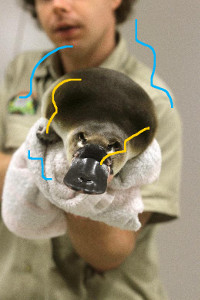
\includegraphics[height=0.35\textheight]{images/etat-de-l-art/region-based-method}
		 \caption{Binarisation interactive par recherche des régions : exemple de \modif{germes donnés} par l'utilisateur.}
		 \label{fig:sota_region_based_ihm}
\end{figure}

\modif{Notons que le fait de tracer des traits n'est pas le seul moyen pouvant être utilisé pour donner les germes \cite{friedland2005siox,rother2004grabcut}.}


Le principal défaut de ce \modif{type d'indications} est qu'il nécessite que l'utilisateur sache quels pixels permettront à la méthode de binarisation interactive de distinguer au mieux la forme du fond. Par exemple, sur la figure \ref{fig:sota_region_based_ihm}, le fait qu'aucun germe \modif{n'ait été placé sur les} cheveux de la personne en arrière plan risque de produire une segmentation erronée, où ces cheveux seront confondus avec le pelage de l'ornithorynque.

\subsection{Méthode de Boykov \textit{et al.}}
\label{sec:sota:boykov}
L'algorithme par coupure de graphe de Boykov \textit{et al.} \cite{boykov2001interactive} cherche la segmentation $S^{*}$ qui minimise \modif{$\mathcal{F}_{C}$} en utilisant un algorithme de maximisation de flot sur un graphe $\mathcal{G}'=\ <V',E'>$, créé à partir de $\mathcal{G}$,  avec :
\begin{itemize}
\item l'ensemble de sommets \modif{$V' = V \cup \lbrace  v_{S}, v_{P} \rbrace$, où $v_{S}$ et $v_{P}$} sont deux sommets spéciaux, la source et le puits ;
\item l'ensemble d'arêtes \modif{$E^{'} =  E \cup E_{S} \cup E_{P}$, où $E_{S}$ est composé des arêtes reliant chaque sommet de $V$ à $v_{S}$ et $E_{P}$ est composé des arêtes reliant chaque sommet de $V$ à $v_{P}$}.
\end{itemize}

Soit $I(p_{i})$ le niveau de gris du \modif{$i\ieme$} pixel  et $P(i,\lambda)$, la probabilité pour ce pixel d'appartenir à la classe de label $\lambda$. Chaque arête $e_{i,j} \in E$ reçoit une pondération inversement proportionnelle à la distance euclidienne entre les positions des \modif{$i\ieme$ et $j\ieme$} pixels ainsi qu'à la différence de leurs niveaux de gris, ce qui permet de s'assurer que des pixels voisins et similaires soient regroupés dans la même région. La pondération de chaque arête \modif{$e_{i,P} \in E_{S}$ (respectivement $e_{i,S} \in \modif{E_{P}}$)}  est inversement proportionnelle à la probabilité que le \modif{$i\ieme$} pixel appartienne à l'objet (respectivement au fond) sachant son niveau de gris. Ces probabilités sont calculées à partir de l'analyse des distributions des niveaux de gris des germes attribués à chacune des classes.  Le tableau \ref{tab:sota:areteBoykov} récapitule\modif{, pour chaque type d'arête,} la \modif{fonction permettant} de calculer sa pondération. 
\begin{table}
\centering
\begin{tabular}{|p{1cm}|p{7cm}|p{5cm}| }
\hline
\textbf{Arête}&\textbf{Type d'arête}&\textbf{\modif{Pondération}}\\
\hline
$e_{i,j}$ &$e_{i,j} \in E$& $\exp\left(\dfrac{-(I(p_{i}) -I(p_{j}))^{2}}{2\sigma^{2}}\right)$\\
\hline
$e_{i,S}$ &le \modif{$i\ieme$} pixel  n'est pas un germe& $- \ln(P(i,\lambda_{F})) $\\
$e_{i,S}$ &le \modif{$i\ieme$} pixel  est un germe de label $\lambda_{O}$&$+\infty$ \\
$e_{i,S}$ & le \modif{$i\ieme$} pixel  est un germe de label $\lambda_{F}$&$0$\\
\hline
$e_{i,P}$ &le \modif{$i\ieme$} pixel n'est pas un germe&$ - \ln(P(i,\lambda_{O}))$\\
$e_{i,P}$ & le \modif{$i\ieme$} pixel  est un germe de label $\lambda_{O}$&$0$ \\
$e_{i,P}$ &le \modif{$i\ieme$} pixel est un germe de label $\lambda_{F}$& $+\infty$\\
\hline
\end{tabular}
\caption{Pondération des arêtes dans l'algorithme de Boykov \textit{et al.} \cite{boykov2001interactive}.}
\label{tab:sota:areteBoykov}
\end{table}

Une \modif{manière intuitive} de produire une binarisation de $I$ à partir de sa représentation $\mathcal{G}'$ consiste à retirer les arêtes de plus faibles pondérations jusqu'à obtenir deux composantes connexes, l'une contenant la source et l'autre le puits : dans ce cas, il s'agit de trouver une coupe minimale de $\mathcal{G}$. Or ce problème est équivalent à la recherche d'un flot maximum, problème pour lequel Boykov \textit{et al.} proposent un algorithme permettant de trouver efficacement une solution. Afin d'obtenir une binarisation de l'image, il suffit alors d'attribuer le label $\lambda_{O}$ à tous les pixels rattachés à la source et le label $\lambda_{F}$ à ceux rattachés au puits. 

 \subsection{Méthode de Jian \textit{et al.}}
\label{sec:sota:jian}
Contrairement aux approches précédemment décrites qui travaillent à l'échelle du pixel,  l'algorithme de Jian \textit{et al.} \cite{jian2016interactive} utilise une sur-segmentation de l'image, où les pixels sont groupés en petites régions homogènes, nommées \emph{superpixels}. Ces superpixels sont produits grâce à l'algorithme mean-shift \cite{comaniciu2002mean}, qui permet de réduire considérablement le nombre de primitives visuelles à manipuler, en créant des ensembles de pixels adjacents dont les couleurs sont similaires. Un exemple visuel du résultat de cette compression est donné sur la figure \ref{fig:sota:meanshift}.

\begin{figure}[htb]
	\centering
	 \begin{subfigure}[t]{0.45\textwidth}	
			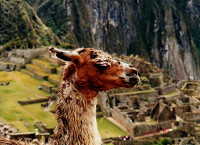
\includegraphics[width=\textwidth]{images/etat-de-l-art/meanshit_im}
		 \caption{Image originale. }
			\label{fig:sota:app_contexts_rv}
	\end{subfigure}
	~
	 \begin{subfigure}[t]{0.45\textwidth}	
			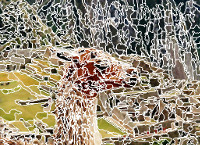
\includegraphics[width=\textwidth]{images/etat-de-l-art/meanshit_ex}
		 \caption{Superpixels produits par l'algorithme mean-shift.}
			\label{fig:sota:app_contexts_ocr}
	\end{subfigure}
	~
	\caption{Compression des pixels en superpixels avec l'algorithme mean-shift.}
	\label{fig:sota:meanshift}
\end{figure}

Jian \textit{et al.} choisissent de décrire chaque superpixel par son histogramme de couleurs normalisé. Afin de réduire la dimension du descripteur correspondant à cet histogramme, chaque canal de couleur est quantifié en $16$ ensembles de taille identique. 

Soit $\mathbb{S} = \lbrace \mathbf{s}_{1} , \cdots  \mathbf{s}_{N_{\mathbb{S}}} \rbrace$ l'ensemble des descripteurs de ces superpixels. À partir de $G$, \modif{l'ensemble $G'$ est obtenu. Ses} éléments sont des couples de la forme \modif{$( \mathbf{s}_{i},\lambda_{j})$} associant aux superpixels contenant des germes, le label correspondant.  \modif{Les superpixels contenant à la fois des germes de label $\lambda_{O}$ et de label $\lambda_{F}$ sont écartés. Soit $N_{G'}$ le nombre de superpixels contenant des germes pour une seule classe : }l'ensemble $\mathbb{S}$ peut alors être ordonné, de manière à ce que les $N_{G'}$ superpixels \modif{de l'ensemble $G'$ constituent} ses $N_{G'}$ premiers éléments. 

Soit $\mathbb{S}_{M}$ l'ensemble des couples de superpixels rattachés à la même classe, c'est-à-dire que \modif{:}
\modif{
\begin{equation}
(\mathbf{s}_{i1},\mathbf{s}_{i2}) \in \mathbb{S}_{M} \Rightarrow (\mathbf{s}_{i1},\lambda_{j1}) \in G' \wedge  (\mathbf{s}_{i2},\lambda_{j2}) \in G' \wedge \lambda_{i1}=\lambda_{i2}\text{.}
\end{equation}
}

Soit $\mathbb{S}_{C}$ l'ensemble des couples de superpixels rattachés à des classes différentes\modif{, c'est-à-dire que : 
\begin{equation}
(\mathbf{s}_{i1},\mathbf{s}_{i2}) \in \mathbb{S}_{C} \Rightarrow (\mathbf{s}_{i1},\lambda_{j1}) \in G' \wedge  (\mathbf{s}_{i2},\lambda_{j2}) \in G' \wedge \lambda_{i1} \neq \lambda_{i2}\text{.}
\end{equation}
}

Les éléments de la matrice de \modif{contraintes} $M_{M}$ sont définis de la manière suivante : 
\modif{
\begin{equation}
M_{M}(i,j) = \begin{cases} ( \mathbf{s}_{i}- \mathbf{s}_{j})( \mathbf{s}_{i}- \mathbf{s}_{j})^{\top}  &\text{ si } ( \mathbf{s}_{i}, \mathbf{s}_{j}) \in \mathbb{S}_{M} \\
 0 &\text{ sinon.}
\end{cases}
\end{equation}
}

De même, les éléments de la matrice de contrainte $M_{C}$ sont définis par :
\modif{
\begin{equation}
M_{C}(i,j) =\begin{cases} ( \mathbf{s}_{i}- \mathbf{s}_{j})( \mathbf{s}_{i}- \mathbf{s}_{j})^{\top}  &\text{ si } (\mathbf{s}_{i},\mathbf{s}_{j}) \in \mathbb{S}_{C} \\
0 &\text{ sinon.}
\end{cases}
\end{equation}
}

\modif{Soient} $N_{\mathbb{S}}$ le nombre de superpixels et \modif{$M_{Id}$} la matrice identité de dimension $N_{\mathbb{S}} \times N_{\mathbb{S}}$. La matrice d'affinité entre les superpixels est une matrice carrée $M_{A}$ de dimension $N_{\mathbb{S}} \times  N_{\mathbb{S}}$, dont l'élément $M_{A}(i,j)$ correspond à une mesure de la similarité entre les \modif{$i\ieme$ et $j\ieme$} superpixels. Cette mesure est obtenue en utilisant les coefficients de Bhattacharyya :\modif{
\begin{equation}
M_{A}(i,j) = \mathcal{F}_{bha}( \mathbf{s}_{i}, \mathbf{s}_{j}) = \sum_{u=1}^{3 } \sqrt{H_{i}(u)\cdot H_{j}(u)}
\end{equation}
}
avec $H_{i}$ l'histogramme de couleur normalisé pour le $i\ieme$ superpixel et $3$ le nombre de canaux de couleur.

Soit la matrice diagonale $M_{D}$, de dimension $N_{\mathbb{S}} \times N_{\mathbb{S}}$, telle que :
\begin{equation}
M_{D}(i,i) = \sum_{j=0}^{N_{\mathbb{S}}} M_{A}(i,j)\text{.}
\end{equation}

Soit la matrice\modif{:
\begin{equation}
A = \omega_{L}(M_{Id} - M_{D}^{-1/2} M_{A} M_{D}^{-1/2}) + \omega_{\alpha} M_{M} - \omega_{\beta} M_{C}
\end{equation}
avec $\omega_{L}$, $\omega_{\alpha}$, $\omega_{\beta}$ des pondérations.}

\modif{La matrice $A$ est décomposée en : }
\begin{equation}
A = 
\begin{bmatrix}
A_{1} & A_{2}\\
A_{3} & A_{4}
\end{bmatrix}
\end{equation}
avec $A_{1}$ de dimension $N_{G'} \times N_{G'}$, $A_{2}$ de dimension $N_{G'} \times ( N_{\mathbb{S}} - N_{G'})$, $A_{3}$ de dimension $( N_{\mathbb{S}} - N_{G'}) \times  N_{G'}$ et $A_{4}$ de dimension $( N_{\mathbb{S}} - N_{G'}) \times ( N_{\mathbb{S}} - N_{G'})$.
À partir de ces  contraintes et \modif{de la matrice d'affinité $M_{A}$}, la structure discriminative globale de l'image est apprise et les germes sont propagés suivant l'algorithme 
\ref{algo:sota:ACP}.

\begin{algorithm}
\caption{Calcul de la structure discriminative globale d'une image\\
}
\label{algo:sota:ACP}
\begin{algorithmic}[1]
\State Calculer \modif{la matrice laplacienne} $L = M_{Id} - M_{D}^{-1/2} M_{A} M_{D}^{-1/2}$
\State Créer la matrice \modif{l}aplacienne contrainte $A$
\State Séparer $A$ en 4 sous-matrices 
\State Trouver la matrice $K_{1}^{*}$ qui minimise \modif{$\tr\left((A_{1}-A_{2}A_{4}^{-1}A_{3}^{\top})K_{1}\right) $} sous la contrainte \modif{: ${K_{1}(i,i) = 1}$}, avec \modif{$\tr(M)$} la trace de la matrice $M$.
\State Propager $K_{1}^{*}$ pour obtenir \modif{$K^{*}= \begin{bmatrix}
K_{1}^{*} & -K_{1}^{*}A_{3}A_{1}^{-1} \\
-A_{1}^{-1}A_{3}^{\top}K_{1}^{*} & -A_{1}^{-1}A_{3}^{\top}K_{1}^{*}A_{3}-A_{1}^{-1}
\end{bmatrix} $}
\end{algorithmic}
\end{algorithm}

 Les colonnes de la matrice $K^{*}$ à l'issue de cette étape correspondent à de nouveaux descripteurs, avec un descripteur pour chaque superpixel. Afin de produire la segmentation finale, ils sont groupés en deux ensembles grâce à l'algorithme des \modif{$k$}-moyennes. 


\subsection{Méthode de Salembier \textit{et al.}}
\label{subsec:sota:salembier}
L'algorithme de Salembier \textit{et al.} \cite{salembier2000binary} utilise une segmentation hiérarchique de l'image, représentée sous la forme d'un \modif{arbre binaire de partition} (ABP). 

Soit $R^{0}=\lbrace r^{0}_{0}, \cdots, r^{0}_{N_{I}} \rbrace$ une partition initiale de l'image, où chaque pixel correspond à une composante connexe $r_{i}^{0}$. Soit $f_{d}(r_{i}^{m},r_{j}^{n})$, une fonction calculant le degré de \modif{dissimilarité} entre deux régions $r_{i}^{m}$ et $r_{j}^{n}$\modif{. Les indices $m$ et $n$ représentent le niveau de chaque région dans l'arbre.} La segmentation hiérarchique utilisée par l'algorithme de Salembier \textit{et al.} est obtenue en fusionnant les deux régions qui \modif{minimisent} $f_{d}$, jusqu'à ce qu'un critère de terminaison (par exemple un nombre de composantes connexes) soit atteint.

Un ABP est un arbre dont les feuilles correspondent aux composantes connexes de $R^{0}$ et où un nœud est ajouté \modif{dès} qu'une fusion est réalisée.  La figure \ref{fig:sota:ABP} donne un exemple d'ABP obtenu à partir de l'image de la figure \ref{fig:sota::img_graph1}. Dans cet exemple, chaque composante connexe est décrite par la couleur moyenne de ses pixels. La fonction $f_{s}$ utilisée \modif{est la distance euclidienne entre les couleurs associées aux} deux composantes connexes. Le critère d'arrêt est l'obtention d'une composante connexe regroupant tous les pixels de l'image.

\begin{figure}[htb]
	\centering
			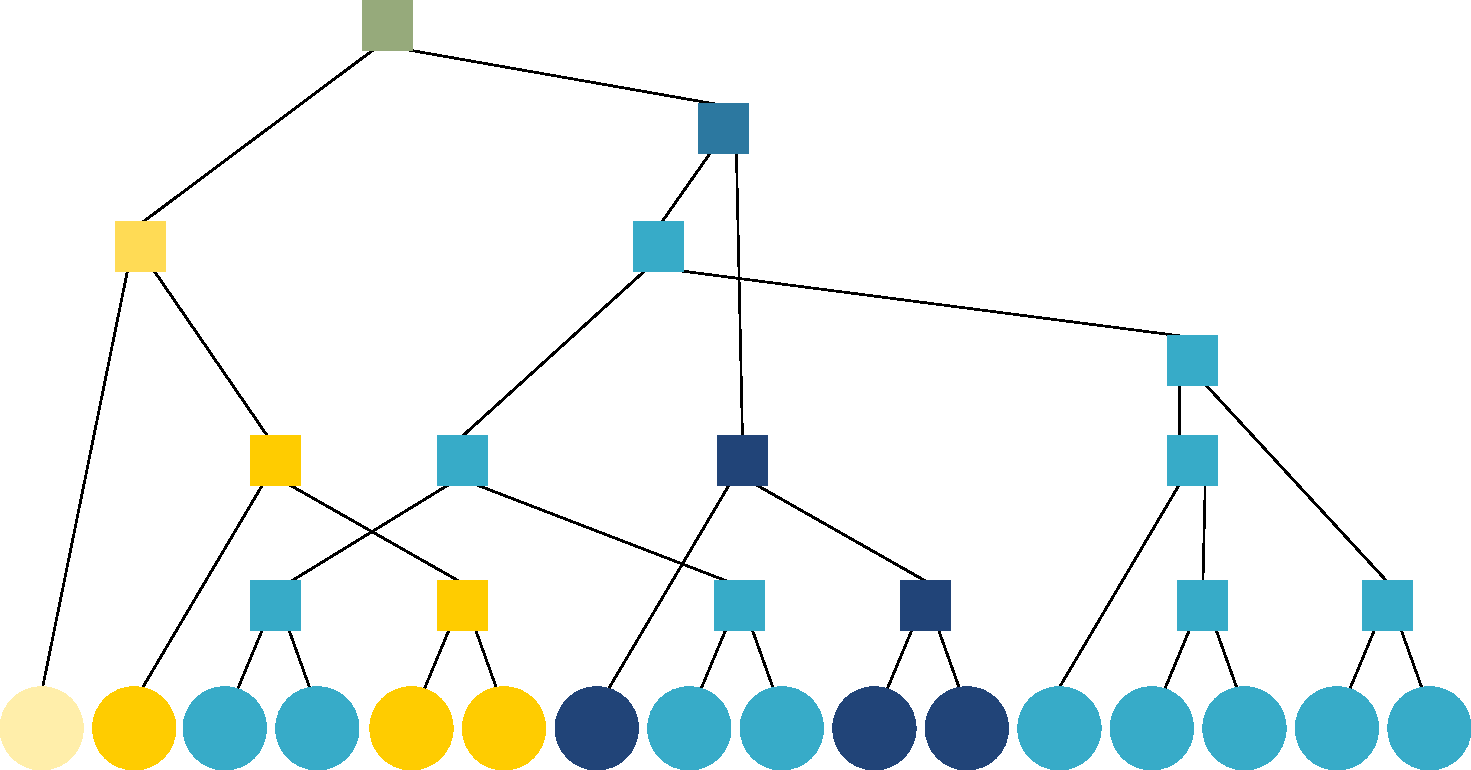
\includegraphics[width=0.45\textwidth]{images/etat-de-l-art/ABP}
		 \caption{ABP obtenu après fusion des pixels de l'image de la figure \ref{fig:sota::img_graph1}.}
		 \label{fig:sota:ABP}
\end{figure}

Salembier \textit{et al.} décrivent chaque région $r_{i}^{m}$ par sa couleur $c_{i}^{m}$, exprimée dans l'espace CIELuv. La conversion de la couleur d'un pixel depuis l'espace RVB vers l'espace CIELuv est donnée par :

\begin{equation}
\begin{bmatrix}
L \\ u \\ v
\end{bmatrix}
=
\begin{bmatrix}
 116f_{luv}(Y/Y_{n}) - 16 \\
 13L(\frac{4X}{X+15Y+3Z} -u_{n}) \\
 13L(\frac{9Y}{X+15Y+3Z} - v_{n})
\end{bmatrix}
\end{equation}
avec  $Y_{n}$, $u_{n}$ et $v_{n}$ les valeurs pour le blanc de référence. Les variables  $X$, $Y$ et $Z$ correspondent à la conversion depuis l'espace RVB vers l'espace de CIEXYZ :
\begin{equation}
\begin{bmatrix}
X \\ Y \\ Z
\end{bmatrix}
= 
\begin{bmatrix}
 2,7689 & 1,7517 & 1,1302 \\
 1 & 4,5907 & 0,601 \\
 0 & 0,056508 &5,5943
\end{bmatrix}
\begin{bmatrix}
R \\ V \\ B
\end{bmatrix}
\end{equation} et 
\modif{
\begin{equation}
f_{luv}(t) = \begin{cases} t^{1/3} &\text{ si } t > \left(\frac{6}{29}\right)^{3} \\
\frac{1}{3}\left(\frac{29}{6}\right)^{2}t + \frac{4}{29} &\text{ sinon}.
 \end{cases}
 \end{equation}}
Lorsque deux régions $r_{i}^{m}$  et $r_{j}^{n}$ sont fusionnées, elles forment une nouvelle région $r _{i \cup j}^{\max(m,n)+1}$ dont le niveau dans l'arbre est égal au niveau le plus élevé des deux anciennes régions \modif{augmenté de} $1$. La couleur de cette nouvelle région est égale à :
\begin{equation}
c_{i \cup j}^{\max(m,n)+1} = \begin{cases}  c_{i}^{m} &\text{ si } |r_{i}^{m}| >  |r_{j}^{n}| \\
 c_{j}^{n} &\text{ si } |r_{j}^{n}| >  |r_{i}^{m}| \\
 \dfrac{c_{i}^{m}+c_{j}^{n}}{2} &\text{ si } |r_{i}^{m}| =  |r_{j}^{n}| 
\end{cases}
\end{equation}
avec $|r_{i}^{m}|$ la cardinalité de la région $r_{i}^{m}$. La fonction de \modif{dissimilarité} entre deux régions est égale à :
\modif{
\begin{equation}
f_{d}(r_{i}^{m},r_{j}^{n}) = |r_{i}^{m}|\times ||c_{i}^{m} - c_{i \cup j}^{\max(m,n)+1}|| + |r_{j}^{n}|\times ||c_{j}^{n} - c_{i \cup j}^{\max(m,n)+1}||
\end{equation}
}
\modif{où $ ||.|| $ désigne} la norme \modif{euclidienne}.


L'algorithme de Salembier \textit{et al.}  commence par propager les germes donnés par l'utilisateur des feuilles de l'ABP jusqu'à sa racine. Si deux labels différents remontent vers un même nœud, celui-ci est noté comme \emph{instable}. Dans une seconde étape, les labels sont à nouveau propagés, de la racine vers les feuilles, en partant des nœuds qui ne sont pas marqués comme \emph{instables}. \modif{À} l'issue de ces deux étapes, certains nœuds ou feuilles peuvent demeurer sans label. Les régions correspondant à ces nœuds reçoivent le label d'une des régions qui leur est adjacente. Si la région non classée comprend plusieurs régions adjacentes avec des labels différents, le label de la région la plus proche au sens d'une mesure de similarité lui est attribué. \modif{Salembier \textit{et al.} n'indiquant pas de mesure de similarité particulière, McGuinness \textit{et al.} \cite{mcguinness2010comparative}, dans leurs travaux visant à évaluer différentes méthodes de binarisation interactive par recherche des régions, proposent d'utiliser la distance euclidienne entre les couleurs moyennes des régions, exprimées dans l'espace CIELuv.}

\subsection{Méthode de Friedland \textit{et al.}}

L'algorithme SIOX \cite{friedland2005siox}, proposé par de Friedland \textit{et al.}, sépare un objet du fond en analysant \modif{leurs signatures de couleurs}. 

\modif{Soient $X = \lbrace x_{1}, \cdots x_{N_{X}} \rbrace$ un ensemble discret de valeurs possibles} et $A=\lbrace a_{1}, \cdots a_{N_{A}} \rbrace$ un ensemble discret de $N_{A}$ éléments, tel que $\forall i \in [1,N_{A}]$, $a_{i} \in X$. Nous notons $H_{X,A}$,  l'histogramme \modif{des valeurs prisent par les éléments de l'ensemble $A$}. Cet histogramme est une liste ordonnée \modif{de $N_{X}$} entiers naturels \modif{qui sont le nombre} d'occurrences de chaque valeur $x_{i} \in X$ dans l'ensemble $A$. \modif{Soit $H_{X,A}(x_{i})$, ce nombre d’occurrences pour la valeur $x_{i} \in X$.}

La fonction $\signature(H_{X,A})$ \modif{donne} la signature \modif{de} l'histogramme $H_{X,A}$, c'est-à-dire un ensemble de $N_{sign}$ paires $(w_{i},m_{i})$ telles que :
\begin{itemize}
\item $N_{sign} \leq N_{X}$ ;
\item \modif{$w_{i} = x_{i} \Rightarrow H_{X,A}(x_{i}) > 0 $}  ;
\item $m_{i} = H_{X,A}(w_{i})$.
\end{itemize}
La signature peut donc être vue comme une version compressée d'un histogramme où les \modif{valeurs de $X$} non représentées sont absentes. 

\modif{
Soit $I$ une image couleur. À chaque pixel est associé un vecteur de trois réels qui correspondent aux valeurs de ce pixel pour chaque canal de couleur $ [c_{1}, c_{2}, c_{3}]$.  Soit $A'$, un sous-ensemble des pixels appartenant à $I$.  L'histogramme $H_{c_{k},A'}$ correspond à l'histogramme des valeurs prises par les pixels de  $A'$, pour le canal de couleur $c_{k}$. Le nombre de classes pour cet histogramme est égal  à $N_{c_{k}}$, le nombre de valeurs possibles pour le canal de couleur $c_{k}$. Plus ce nombre est important, plus la distinction entre les différentes couleurs est précise. Nous obtenons donc trois histogrammes  ($H_{c_{1},A'}$, $H_{c_{2},A'}$, $H_{c_{3},A'}$), avec chacun un nombre de classes qui lui est propre et qui dépend de la précision souhaitée sur chaque canal de couleur. Ces histogrammes et les signatures qui leur sont associées sont calculés pour le fond et pour la forme, à partir des germes donnés par l'utilisateur.}

Chaque pixel de l'image est ensuite attribué au fond ou à l'objet à extraire en fonction de la signature à laquelle sa couleur appartient. Si la couleur du pixel n'appartient à aucune des signatures, il est attribué à la classe dont la signature contient la couleur la plus proche, \modif{au sens de la distance euclidienne}.

Le nombre de classes pour les histogrammes est un paramètre fixé par l'utilisateur. Il peut varier d'une composante colorimétrique à l'autre et selon la complexité de l'image. 

\section{Méthodes de segmentation interactive \modif{multiclasse}}

\subsection{Formulation du problème}

Le problème de la segmentation interactive \modif{multiclasse} peut se voir comme une généralisation de celui de la binarisation interactive par recherche des régions, la principale différence résidant dans le fait que le nombre de classes \modif{est variable d'une image à l'autre}. L'ensemble des labels possibles devient donc : \modif{$\Lambda = \lbrace \lambda_{1}, \cdots \lambda_{N_{\Lambda}} \rbrace$}. La segmentation obtenue correspond toujours à une partition \modif{$S$} de l'image en régions, avec une ou plusieurs régions pouvant être attribuées à chaque classe.

L'une des approches les plus courantes pour résoudre ce type de problème consiste à trouver la segmentation $S$ minimisant la fonction de Potts : 
\modif{
\begin{equation}
\label{eq:sota:pott}
\mathcal{F}_{Potts}(I,G,S) =  \omega \sum_{i=1}^{N_{I}} \mathcal{F}_{D}(p_{i},\lambda_{j}) + \dfrac{1}{2} \sum_{i=1}^{N_{S}} \mathcal{F}_{R}(I,S_{i}) 
\end{equation}
}
où :
\begin{itemize}
\item \modif{$F_{R}$} est un terme de régularisation
\begin{itemize}
\item  pénalisant les segmentations $S$ comprenant des régions aux contours sinueux ;
\item favorisant l'alignement des contours des régions sur les contours de l'image ;
\end{itemize}
\item \modif{$F_{D}$ est le terme d'attache aux données évaluant la pertinence d'attribuer le label $\lambda_{j}$ au pixel $p_{i}$, en fonction des caractéristiques de l'image $I$ et des germes $G$};
\item \modif{$\omega$ est un paramètre pondérant l'influence du terme d'attache aux données.}
\end{itemize}

\subsection{Interaction avec l'utilisateur}

Comme le montre la figure \ref{fig:sota_region-based-method-mc-ihm}, le mode d'interaction avec l'utilisateur est proche de celui employé pour les méthodes de binarisation interactive par recherche des régions, seul change le nombre de couleurs disponibles, lequel n'est plus limité à deux.

\begin{figure}[htb]
	\centering
			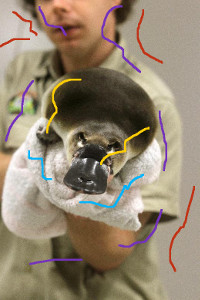
\includegraphics[height=0.35\textheight]{images/etat-de-l-art/region-based-method-mc}
		 \caption{Segmentation interactive \modif{multiclasse} par recherche des régions : exemple d'indications données par l'utilisateur.}
		 \label{fig:sota_region-based-method-mc-ihm}
\end{figure}




\subsection{Méthode d'Adams \textit{et al.}}

L'algorithme d'Adams \textit{et al.} \cite{adams1994seeded} fait partie des méthodes de segmentation interactive les plus anciennes. Toutefois\modif{,} sa grande simplicité en fait une méthode de segmentation interactive \modif{multiclasse} parmi  les plus rapides.

 Soit $V_{G} \subset V $, tel que $v_{i} \in  V_{G} \Leftrightarrow \exists (p_{i},\lambda_{j}) \in G$, l'ensemble des sommets correspondant à des germes. Soit $A= \lbrace A_{1}, \cdots, A_{N_{CC}} \rbrace $  une partition de $V_{G}$ en $N_{CC}$ composantes connexes, de manière à ce que tous les sommets rattachés à une même composante connexe correspondent à des germes de même label. \modif{Soit $\overline{V_{G}}$ l'ensemble complémentaire de $V_{G}$}. 
 
Adams \textit{et al.} proposent un algorithme itératif où, à chaque étape, un sommet de \modif{$\overline{V_{G}}$} est attribué à l'une des composantes connexes de $A$, jusqu'à que l'ensemble \modif{$\overline{V_{G}}$} soit vide. Le sommet sélectionné doit \modif{correspondre à un pixel voisin de} l'un des pixels de $V_{G}$ et \modif{satisfaire} un critère de similarité avec l'une des composantes connexes. Lorsqu'il est attribué, il est retiré de \modif{$\overline{V_{G}}$} et ajouté à $V_{G}$.

La similarité entre un pixel $p_{i}$ et une composante connexe $A_{j}$ \modif{est estimée à partir de la distance} euclidienne entre la couleur de $p_{i}$ et la couleur moyenne des pixels attribués à $A_{j}$, les couleurs étant exprimées dans l'espace CIELuv.


\subsection{Méthode de Santner \textit{et al.}}
\label{sec:sota:santner}

Dans leur article \cite{santner2010interactive}, Santner \textit{et al.} proposent de trouver une segmentation optimale de l'image en minimisant la fonction de Potts, définie par l'équation \ref{eq:sota:pott}.

Le terme d'attache aux données, \modif{$\mathcal{F}_{D}$} correspond à la probabilité de chaque pixel d'appartenir à chacune des classes. Cette probabilité est obtenue en utilisant une \modif{forêt aléatoire} (FA) \cite{breiman2001random}, qui est une méthode d'apprentissage consistant à combiner les résultats de plusieurs arbres décisionnels.

Un arbre décisionnel est un modèle prédictif reposant sur un ensemble de règles binaires. Présentée à un nœud, la donnée à classer est orientée vers le fils droit ou le fils gauche, en fonction de ses caractéristiques. L’arrivée sur une feuille de l’arbre correspond à une prise de décision. Afin de pouvoir classer correctement une donnée, l’arbre doit être paramétré lors d’une étape d’apprentissage, à partir de données dont la classe est connue. La phase d’apprentissage consiste à déterminer pour chaque nœud un hyperplan dans un espace à $m$ dimensions, $m$ étant le nombre d’attributs utilisés par ce nœud, inférieur ou égal au nombre d’attributs caractérisant une donnée. Durant la phase d’exploitation, lorsqu’une donnée arrive sur un nœud, les valeurs des attributs pris en compte par ce nœud permettent de la positionner dans l’espace à $m$ \modif{dimensions} : selon sa position vis-à-vis de l’hyperplan, la donnée est envoyée vers le fils droit ou vers le fils gauche.

Dans le cas d’un classificateur de type FA, chaque arbre décisionnel est entraîné à partir d’une partie des données d’apprentissage, prélevée de manière aléatoire. En phase d’exploitation, lorsqu’une donnée est fournie à la FA, chaque arbre vote pour la classe qui lui semble la plus adéquate.
Pour chacune des classes, il est alors possible de connaître le nombre d’arbres décisionnels qui ont voté en sa faveur et d’en déduire la probabilité que la donnée appartienne à cette classe.


L'algorithme de Santner \textit{et al.} utilise les germes comme données d'apprentissage. Chaque pixel est décrit par sa couleur exprimée dans l'espace $CIELab$ et un identifiant caractérisant \modif{la texture en son voisinage}, \modif{nommé motif binaire local, en anglais \og \textit{local binary pattern}\fg} (LBP) \cite{ojala2002multiresolution}.

Soit $p_{i}$ un pixel de niveau de gris \modif{$I(p_{i})$} et \modif{$\lbrace I(p_{i}^{0}), \cdots, I(p_{i}^{P-1})\rbrace$} les niveaux de gris des $P$  voisins de $p_{i}$ répartis régulièrement sur le cercle de centre $p_{i}$ et de rayon $R$. L'identifiant LBP de $p_{i}$ est égal à : 
\modif{\begin{equation}
LBP_{R,P}(i) = \sum_{j=0}^{P-1} \tau (I(p_{i}) - I(p_{i}^{j})) 2^{j}
\end{equation}}
avec  $\tau$ une fonction seuil renvoyant $0$ si son argument est strictement négatif, $1$ sinon.

La conversion d'une couleur de l'espace RVB à l'espace CIELab est donnée par :
\begin{equation}
\begin{bmatrix}
L \\ a \\ b
\end{bmatrix}
=
\begin{bmatrix}
 116f_{lab}(Y/Y_{n}) - 16 \\
 500f_{lab}(\frac{X}{X_{n}} - \frac{Y}{Y_{n}}) \\
 200f_{lab}(\frac{Y}{Y_{n}} - \frac{Z}{Z_{n}}) 
\end{bmatrix}
\end{equation}
avec $X_{n}$, \modif{$Y_{n}$} et \modif{$Z_{n}$} correspondant aux valeurs pour le blanc de référence, $X$, $Y$ et $Z$  le passage de  l'espace RVB vers l'espace CIEXYZ, décrit dans la section \ref{subsec:sota:salembier}, et 
\modif{
\begin{equation}f_{lab} = \begin{cases} t^{1/3} &\text{ si } t > \left(\frac{6}{29}\right)^{3} \\
\frac{1}{3}\left( \frac{29}{6}\right)^{2}t + \frac{4}{29} &\text{ sinon}.
 \end{cases}\end{equation}}

Pour le terme de régularisation \modif{$\mathcal{F}_{R}$}, le calcul du gradient permet d'obtenir pour chaque pixel sa probabilité d'appartenir à un contour de l'image. 
 
Une fois le problème de la minimisation de la fonction de Potts reformulé en problème d'optimisation convexe grâce  à l'approche de relaxation convexe de Pock \textit{et al.} \cite{pock2009convex}, une approximation de la solution est trouvée en utilisant un algorithme de type \emph{primal-dual} \cite{boyd2004convex}. 

\subsection{Méthode de \modif{Müller} \textit{et al.}}
\label{subsec:sota:muller}
À l'instar de Santner \textit{et al.} \cite{santner2010interactive}, \modif{Müller} \textit{et al.} \cite{muller2016robust} cherchent une segmentation de l'image par minimisation de la fonction de Potts, dont la forme générale est donnée par l'équation \ref{eq:sota:pott}. 

Soit \modif{$f_{c}$} la fonction associant à chaque pixel $p_{i}$ sa couleur dans un espace colorimétrique donné et \modif{$f_{l}$} la fonction associant à chaque pixel ses coordonnées dans l'image. Le terme d'attache aux données \modif{$\mathcal{F}_{D}$}  de \modif{Müller} \textit{et al.} \cite{muller2016robust} s'inspire des travaux de Nieuwenhuis \textit{et al.} \cite{nieuwenhuis2013spatially}, avec :
\modif{
\begin{equation}
\mathcal{F}_{D}(p_{i},\lambda_{j}) = - \log(P(p_{i} | \lambda_{j}))
\end{equation}
}
où $P(p_{i} | \lambda_{j})$ est la probabilité conjointe d'avoir un pixel de couleur $f_{c}(p_{i})$ et de localisation $f_{l}(p_{i})$ sachant que le label $\lambda_{j}$ \modif{lui est attribué}.  Soit $G^{\lambda_{j}}$ l'ensemble des germes pour la classe de label $\lambda_{j}$ : 
\modif{
\begin{equation}
P(p_{i} | \lambda_{j}) = \frac{1}{N_{G^{\lambda_{j}}}} \sum_{k=1} ^{|G^{\lambda_{j}}|} \mathcal{K}_{l} \Big( f_{l}(p_{i}) - f_{l}(p_{k}) \Big) \mathcal{K}_{c} \Big( f_{c}(p_{i}) - f_{c}(p_{k}) \Big)
\end{equation}}
avec $|G^{\lambda_{j}}|$  la cardinalité de l'ensemble $G^{\lambda_{j}}$\modif{,} $\mathcal{K}_{l}$ et $\mathcal{K}_{c}$ deux noyaux \modif{gaussiens de} paramètres différents. Le fait que les deux noyaux gaussiens soient de largeurs différentes permet de pondérer l'influence de chacune des deux informations (la couleur et la localisation).

Alors que Nieuwenhuis \textit{et al.} \cite{nieuwenhuis2013spatially} supposent que les germes sont corrects,  \modif{Müller} \textit{et al.} introduisent dans le calcul de \modif{$\mathcal{F}_{D}$}  la probabilité $P_{corr}((p_{i},\lambda_{j}), k)$ qu'un germe appartienne \modif{bien} à la classe $k$ :
\begin{align*}
P_{corr}((p_{i},\lambda_{j}), k)=  \begin{cases}
\zeta &\text{ si } \lambda_{j}=k \\
\dfrac{(1 - \zeta)}{N_{S} -1} &\text{sinon.}
\end{cases} 
\end{align*}
Le paramètre  $\zeta$ est \modif{la probabilité \textit{a priori} que le germe soit correct. Il  est} fixé de manière empirique par \modif{Müller} \textit{et al.}
 
Le terme de régularisation $\mathcal{F}_{R}$ assure que le périmètre des régions obtenues soit minimal, en intégrant une distance qui ne prend pas seulement en compte le périmètre en termes de nombre de pixels, mais également la probabilité des pixels d'appartenir aux contours de l'image. L'une des particularité des travaux de \modif{Müller} \textit{et al.} \cite{muller2016robust} consiste à utiliser le détecteur de contour de \modif{Doll\'{a}r} \textit{et al.} \cite{dollar2015fast}, donnant un résultat plus précis qu'un simple calcul de gradient. Ce détecteur repose sur  une FA entraînée à  détecter\modif{, dans} un carré de \modif{taille $32 \times 32$, les pixels appartenant à un contour}. 

\begin{emodif}
Chaque pixel de ce carré est décrit par :
\begin{itemize}
\item sa couleur exprimée dans l'espace CIELuv, ce qui donne 3 caractéristiques ;
\item l'amplitude de son gradient, à deux échelles différentes  (échelle $1$ et $\frac{1}{2}$), ce qui donne 2 caractéristiques ;
\item la présence du gradient dans l'une des quatre directions (nord, sud, est, ouest) à deux échelles différentes, ce qui donne 8 caractéristiques.
\end{itemize}
Au total, pour un carré de $32\times32$ pixels, un descripteur de $32\times32\times13$ éléments est obtenu. Afin de réduire la taille de ce descripteur, seule une valeur sur $2$ dans le sens de la hauteur et dans celui de la largeur, est conservée. Le nombre d'éléments est donc ramené à $\frac{32\times32\times13}{4}=3328$.

Ce descripteur est réduit à un carré de $5 \times 5$ pixels et les différences paire à paire entre ces pixels sont également calculées, pour chacune des caractéristiques précédentes (couleur, amplitude et direction du gradient). Ainsi $\binom{5\times5}{2}=300$ différences sont calculées, pour $13$ caractéristiques, ajoutant $3900$  éléments au descripteur. Le descripteur final contient donc $7228$ éléments. 
\end{emodif}


\modif{Müller} \textit{et al.} \cite{muller2016robust} recherchent une segmentation minimisant la fonction de Potts ainsi obtenue en suivant une approche similaire à celle de Santner \textit{et al.}, grâce à un algorithme de type \emph{primal-dual} \modif{\cite{boyd2004convex}}. 
 

\subsection{Méthode de Changjae \textit{et al.}}

L'algorithme de Changjae \textit{et al.} \cite{Changjae2017Robust} résout le problème de la segmentation interactive en produisant un ensemble de $N_{\Lambda}$ fonctions, de la forme $f_{\lambda_{j}}(p_{i},I,G)$. Chaque fonction donne un réel \modif{positif proportionnel} à la probabilité du pixel $p_{i}$ d'appartenir à la classe de label $\lambda_{j}$.

Soit \modif{$f_{c}$} la fonction associant à chaque pixel $p_{i}$ sa couleur dans un espace colorimétrique donné et \modif{$f_{l}$} la fonction associant à chaque pixel ses coordonnées dans l'image. Le degré de ressemblance entre deux pixels $p_{i}$ et $p_{j}$ est donné par : 
\modif{
\begin{equation}
w_{i,j} = \exp \left( - \frac{ ||f_{c}(p_{i}) -f_{c}(p_{j}) ||}{2{\sigma_{c}}^{2}} - \frac{ ||f_{l}(p_{i}) -f_{l}(p_{j}) ||}{2\sigma{_{l}}^{2}} \right)
\end{equation}
}
avec \modif{$\sigma_{c}$ et  $\sigma_{l}$} deux paramètres fixés de manière empirique et dosant l'influence, respectivement, de la couleur et de la localisation du pixel. 

Soit $G^{\lambda_{j}}$ l'ensemble des germes donnés pour la classe de label $\lambda_{j}$. Pour chaque canal de couleur $c_{k}$, Changjae \textit{et al.} calculent $H_{\lambda_{j}}^{c_{k}}(m_{1},m_{2}) $, l'histogramme normalisé de co-occurrence, indiquant la proportion de germes :
\begin{itemize}
\item appartenant à $G^{\lambda_{j}}$ ;
\item ayant une valeur $m_{1}$ pour le canal de couleur $c_{k}$ ;
\item ayant un de leurs voisins dont la valeur\modif{,} pour le même canal\modif{,} vaut $m_{2}$. 
\end{itemize}

Cet histogramme permet d'obtenir :
\modif{
\begin{equation}
P_{\lambda_{j}}^{c_{k}} (m_{1},m_{2}) = \frac{H_{\lambda_{j}}^{c_{k}}(m_{1},m_{2}) }{ \displaystyle \sum_{m_{3} \in M^{c_{k} }} \sum_{m_{4} \in M^{c_{k} }} H_{\lambda_{j}}^{c_{k}}(m_{3},m_{4}) }
\end{equation} 
}
la probabilité d’occurrence et de co-occurrence des valeurs $m_{1}$ et $m_{2}$ pour le canal de couleur  $c_{k}$. L'ensemble $ M^{c_{k}}$ correspond aux valeurs possibles pour le canal de couleur $c_{k}$.  Par exemple, si nous nous intéressons au canal rouge de l'espace RVB, nous aurons  $ M^{rouge}=[0,255]$.

 La probabilité d’occurrence et de co-occurrence  $P_{\lambda_{j}}$\modif{ pour la classe de label $\lambda_{j}$} est obtenue en faisant la moyenne des probabilités d’occurrence et de co-occurrence pour chacun des canaux de couleur.  Cette probabilité permet d'obtenir pour chaque germe $(p_{i},\lambda_{j})$\modif{ :
\begin{equation}
r^{\lambda_{j}}(i) = \sum_{ p_{k} \in \nei(i)} P_{\lambda_{j}}(f_{c}(p_{i}),f_{c}(p_{k}))  \text{,}
\end{equation}}
qui correspond à un score de confiance. La valeur $r^{\lambda_{j}}(i) $  est donc d'autant plus faible que le germe a une probabilité élevée d'être erroné. 

Chaque fonction $f_{\lambda_{j}}$ prend alors la forme d'un vecteur de $N_{I}$ éléments, associant à chaque pixel un réel indiquant son degré d'appartenance à la classe de label $\lambda_{j}$ et défini par
\modif{\begin{equation}
f_{\lambda_{j}}(I,G) = ( D - W + \Omega)^{-1} \Omega R_{j} Z_{j}
\end{equation}}
avec :
\begin{itemize}
\item $D$ une matrice diagonale de taille $N_{I} \times N_{I}$, où le \modif{$i\ieme$} élément de la diagonale vaut $\sum_{j=1}^{N_{I}} w_{i,j} $ ;
\item $W$ une matrice carrée de taille  $N_{I} \times N_{I}$, où l'élément situé sur la ligne $i$ et la colonne $j$ vaut $w_{i,j}$ si le pixel $p_{j}$ fait partie des $K$ plus proches voisins du pixel $p_{i}$ (au sens de la couleur et de la localisation) ou $0$ sinon ;
\item $R_{j}$ une matrice de taille $N_{I} \times N_{I}$, où \modif{le $i\ieme$} élément de la diagonale vaut $r^{\lambda_{j}}(i)$ ;
\item $Z_{j}$ un vecteur de $N_{I}$ éléments, \modif{où le $i\ieme$} élément vaut 1 si le pixel $p_{i}$ est un germe pour la classe de label $\lambda_{j}$, 0 sinon ;
\item \modif{$\Omega$ est une matrice diagonale, dont chaque élément de la diagonale vaut $\omega$, et qui sert à introduire le paramètre $\omega$ régulant l'influence du terme d'attache aux données $\mathcal{F}_{D}$.}
\end{itemize}

\section{Conclusion}

\begin{emodif}
Dans ce chapitre, nous avons présenté le problème de la segmentation interactive. Nous avons notamment décrit une dizaine d'algorithmes proposés durant les deux dernières décennies. Ces méthodes permettent de prendre conscience de la diversité des approches envisagées. 

Certaines méthodes, à l'instar de l'algorithme de Mortensen \textit{et al.} \cite{mortensen1995intelligent} reposent une interactivité forte avec l'utilisateur : chaque fois que ce dernier fournit un nouveau germe, la portion de contour entre celui-ci et le germe précédent est recherchée puis affichée. Cette recherche s'effectue en moins d'une seconde : l'utilisateur, de manière quasi immédiate, voit l'influence du germe qu'il vient de donner. Si le résultat obtenu ne lui convient pas, il peut aisément le modifier. Les deux manipulations principales pour améliorer la courbe (déplacer un germe pour qu'il coïncide davantage avec un point du contour et ajouter un germe entre deux germes précédents pour faciliter la recherche du contour) sont faciles à comprendre. 

D'autres algorithme, comme celui de Müller \textit{et al.} \cite{muller2016robust}, mettent en jeu des traitements plus complexes, tels que l'analyse des germes donnés par l'utilisateur afin de déterminer leur degré de fiabilité. La production d'une segmentation résultat demande des calculs plus nombreux et plus longs : sur des images de quelques milliers de pixels, le temps d'exécution moyen de cette méthode est de 2 secondes, sous réserve d'utiliser une version optimisée tirant profit d'une parallélisation des étapes clés de l'algorithme. 

Si de telles méthodes résolvent indiscutablement des problèmes de vision par ordinateur plus complexes, leur pertinence dans les domaines d'applications qui nous concernent est moins évidente. 

Tout d'abord, rappelons que le cadre des observatoires photographiques du paysage nous impose de réfléchir à des algorithmes capable de fonctionner sur des smartphones, qui disposent de moins de ressources mémoire qu'un ordinateur 
standard, tout en faisant intervenir des processeurs moins puissants. Ensuite, soulignons que dans le cadre d'un logiciel de manipulation d'image tel que Gimp ou Photoshop, les outils de segmentation interactive sont souvent utilisés sur des photographies comprenant au moins plusieurs millions de pixels. Dans ces deux contextes, la complexité d'un algorithme comme celui de Müller est un défaut important. 

Par ailleurs, si le fait de permettre de sélectionner plusieurs objets à la fois (donc de réaliser une segmentation interactive multiclasse) est un avantage par rapport aux méthodes de binarisation interactive, le fait de remettre en cause les indications données par l'utilisateur peut se révéler plus gênant qu'avantageux. En effet, les tests avec des utilisateurs réalisés par McGuinness \textit{et al.} \cite{mcguinness2010comparative} montrent l'importance du caractère prévisible du résultat à partir des germes : en d'autres termes, un algorithme pour lequel l'utilisateur comprendra rapidement l'influence des indications qu'il donne sera généralement mieux accepté qu'une méthode capable de produire, en moyenne, des résultats un peu plus précis, mais ne permettant pas une correction facile lorsqu'elle se trompe. Dans le cas  de Müller \textit{et al.} \cite{muller2016robust}, le fait de ne pas tenir compte de certaines indications, même s'il  permet à l'utilisateur d'être moins précis lorsqu'il donne des germes, peut induire des situations frustrantes où, malgré l'ajout de germes, le résultat n'est pas mis à jour. Ce dernier point est particulièrement vrai lorsque le contraste entre deux objets à sélectionner n'apparaît pas clairement, à cause d'une ombre, d'un problème d'éclairage, etc.

Tous ces éléments nous ont conduit à réfléchir sur un algorithme de segmentation interactive multiclasse qui conserve les deux avantages qui ont fait le succès de méthodes comme celles de Mortensen \textit{et al.} : une faible complexité algorithmique garantissant la production rapide d'un résultat et  l'utilisation de germes dont l'influence est facilement compréhensible par l'utilisateur. Contrairement aux dernières méthodes de segmentation interactive proposées \cite{Changjae2017Robust,muller2016robust,santner2010interactive}, le fonctionnement de cette méthode est itératif, ce qui induit une communication beaucoup plus dynamique avec l'utilisateur.
\end{emodif} 

 
\glsresetall
\chapter{\modif{Algorithme de segmentation interactive Superpixel $\alpha$-Fusion}}

\section{Introduction}
L'une des \modif{principales} contributions \modif{présentée dans ce mémoire est} la proposition d'une nouvelle méthode de segmentation interactive, $S \alpha F$ (Superpixel $\alpha$-Fusion) \cite{mathieu2016segmentation, mathieu2017jei}. Cette méthode permet la sélection précise, intuitive et rapide de multiples objets au sein d'une même photographie. Elle appartient à la catégorie des algorithmes de segmentation interactive \modif{multiclasse} et repose sur une approche par recherche des régions. Les germes donnés par l'utilisateur correspondent à des traits de couleur qui indiquent quelques pixels appartenant à chaque objet à extraire. 

L'algorithme $S \alpha F$ repose sur la modélisation du problème de la segmentation interactive comme la minimisation d'une fonction \modif{de coût} pouvant être représentée par un graphe de facteurs. Il intègre l'utilisation d'une méthode de classification par apprentissage supervisé assurant l'adéquation entre la segmentation produite et les germes donnés, l'introduction d'un nouveau terme de régularisation et la réalisation d'un pré-traitement consistant à regrouper les pixels en petits ensembles cohérents. 

\section{Modélisation du problème de segmentation interactive }

Soit $I$ une image, $\mathbb{S}=\lbrace \mathbf{s}_{1}, \cdots, \mathbf{s}_{N_{\mathbb{S}}} \rbrace$ un ensemble de $N_{\mathbb{S}}$ primitives visuelles, \modif{$\Lambda= \lbrace\lambda_{1},\cdots,\lambda_{N_\Lambda} \rbrace$} un ensemble de \modif{$N_{\Lambda}$} labels correspondant à \modif{$N_{\Lambda}$} classes et $G=\lbrace g_{1}, \cdots, g_{N_{G}} \rbrace$ un ensemble de germes indiquant pour chaque classe quelques pixels lui appartenant. Nous nous intéressons au problème consistant à attribuer, à chaque pixel de $I$, un élément de \modif{$\Lambda$} sous les contraintes suivantes :
\begin{itemize}
\item les pixels possédant le même label doivent former un ensemble visuellement homogène ;
\item la classification produite doit être cohérente vis-à-vis de $G$.
\end{itemize}

Dans le cadre de l'algorithme que nous proposons, chaque primitive visuelle $\mathbf{s}_{i}$ est un ensemble de pixels voisins et similaires,  nommé \emph{superpixel}. Ces ensembles sont construits de manière à ce que l'attribution d'une et \modif{d'}une seule classe à chaque superpixel permette d'obtenir la segmentation recherchée par l'utilisateur.

Les superpixels forment une partition en composantes connexes des pixels de l'image $I$. Ils peuvent donc être représentés par un \modif{graphe} $\mathcal{G}=\ <X,E>$, avec :
\begin{itemize}
\item $X = \lbrace x_{1}, \cdots, x_{N_{\mathbb{S}}}  \rbrace$  un ensemble de sommets, où chaque sommet $x_{i}$ représente un superpixel $ \mathbf{s}_{i}$ ;
\item $E$ un ensemble d'arêtes non orientées, avec une arête $e_{i,j}$ pour chaque paire de superpixels $(\mathbf{s}_{i},\mathbf{s}_{j})$ ayant des pixels \modif{voisins}. 
\end{itemize}

Soit $C=\lbrace c_{1},\cdots,c_{\mathbb{S}} \rbrace$, un ensemble de variables aléatoires indexées par les sommets de $\mathcal{G}$, tel que \modif{$c_{i} \in \Lambda$}. Si nous admettons que la probabilité d'une variable $c_{i}$ de recevoir le label $\lambda_{k}$ ne dépend que des caractéristiques des sommets $x_{j}$ voisins directs de $x_{i}$, alors \modif{$C$} est un \modif{champ aléatoire de Markov} (CAM) et une segmentation optimale \modif{$C^{*}$} s'obtient en minimisant : \modif{
\begin{equation}
\label{eq:safe:mrfprob}
\mathcal{F}_{CAM} (I,C,G) = \sum_{i=1}^{N} \mathcal{F}_{D}(x_{i},c_{i}) \ + \sum_{ e_{i,j} \in E} \omega(x_{i})\mathcal{F}_{R}(x_{i},c_{i},x_{j},c_{j})
\end{equation}}
avec :
\begin{itemize}
\item $\mathcal{F}_{D}$ un terme d'attache aux données, s'assurant de la cohérence \modif{avec les} caractéristiques  \modif{de l'image} $I$ et \modif{celles} des germes $G$ ;
\item $\mathcal{F}_{R}$ un terme de régularisation vérifiant certaines propriétés propres à la segmentation, concernant par exemple  la taille \modif{ou la forme} des régions ;
\item  $\omega$  une fonction de pondération.
\end{itemize}

\subsection{Terme d'attache aux données}

Une segmentation optimale \modif{$C^{*}$} de $I$ étant obtenue par minimisation de $\mathcal{F}_{CAM}$, le terme d'attache aux données \modif{$\mathcal{F}_{D}$} \modif{vaut :} 
\modif{
\begin{equation}
 \mathcal{F}_{D}(x_{i},c_{i}) = 1 -P(\lambda_{j}|x_{i} ) \text{ avec } c_{i} =  \lambda_{j}\text{.} 
\end{equation}
où $P(\lambda_{j}|x_{i} )$ est la probabilité que le sommet $x_{i}$ appartiennent à la classe de label $\lambda_{j}$.
}

\subsubsection{Approche de Wu}
Comme nous nous intéressons à un problème de classification \modif{multiclasse}, \modif{$P(\lambda_{j}|x_{i})$} peut être estimée de manière précise grâce à la seconde des deux méthodes décrites par Wu \textit{et al.}, dans leur article \emph{\og Probability estimates for multi-class classification by pairwise coupling \fg} \cite{wu2004probability}. Elle s'appuie sur le résultat d'une méthode de classification supervisée résolvant des problèmes à deux classes. La fonction binaire associée à cette méthode est $F_{sup}(x_{i},\lambda_{j},\lambda_{k})$ qui vaut :
\begin{itemize}
\item $0$ si les caractéristiques de $x_{i}$ sont plus \modif{proches} \modif{de celles} de la classe $\lambda_{j}$ ;
\item $1$ si les caractéristiques de $x_{i}$ sont plus \modif{proches}  \modif{de celles} de la classe $\lambda_{k}$.
\end{itemize}
L'estimation de la  probabilité que $x_{i}$ appartienne à la classe de label $\lambda_{j}$ plutôt qu'à la classe de label $\lambda_{k}$ est obtenue en calculant :
\modif{
\begin{equation}
F_{jk}(x_{i},\lambda_{j},\lambda_{k}) = \dfrac{1}{1+ \exp(\omega_{A} F_{sup}(x_{i},\lambda_{j},\lambda_{k}) +\omega_{B})}
\end{equation}}
où $\omega_{A}$ et $\omega_{B}$ sont deux paramètres obtenus lors de la phase d'apprentissage de la méthode de classification supervisée. À partir de cette probabilité, Wu \textit{et al.} montrent que la distribution de probabilité \modif{$\mathcal{P}= \lbrace P(\lambda_{1}|x_{i} ), \cdots ,P(\lambda_{N_{\Lambda}}|x_{i} )  \rbrace$} s'estime en minimisant :
\modif{
\begin{equation}
\sum_{j=1}^{N_{\Lambda}} \sum_{\substack{k=1 \\ j \neq k}}^{N_{\Lambda}} \Big( F_{jk}(x_{i},\lambda_{j},\lambda_{k}) P(\lambda_{k}|x_{i} ) - F_{kj}(x_{i},\lambda_{j},\lambda_{k}) P(\lambda_{j}|x_{i} ) \Big)^{2}
\end{equation}
sous les contraintes suivantes :
\begin{itemize}
\item $\displaystyle \sum_{j=1}^{N^{\Lambda}} P(\lambda_{j}|x_{i} ) = 1 $;
\item $P(\lambda_{j}|x_{i} ) \text{ } >0 \ \forall\ j \ \in [1,N_{\Lambda}]$.
\end{itemize}}

\subsubsection{Classification supervisée}
L'utilisation d'une méthode de classification supervisée implique de disposer d'un ensemble de \emph{données d'apprentissage}, permettant de paramétrer la méthode, afin que celle-ci puisse classer les données restantes, nommées \emph{données d'exploitation}. Dans le cas de la méthode que nous proposons, il s'agit de produire une partition de l'ensemble des superpixels \modif{$\mathbb{S}$} associé à une image en deux ensembles : 
\begin{itemize}
\item \modif{$\mathbb{S}_{A}$} pour les données d'apprentissage ;
\item \modif{$\mathbb{S}_{E}$} pour les données d'exploitation.
\end{itemize}
La construction de ces deux ensembles s'effectue par analyse des indications données par l'utilisateur. L'ensemble des germes $G$ étant constitué de couples $(p_{i},\lambda_{j})$, associant un label à certains pixels de l'image $I$, il convient de trouver une procédure à la fois rapide et fiable pour transférer ces germes vers les superpixels. 

Soit $\mathbf{s}_{k}$ un superpixel. Trois cas de figure peuvent se présenter :
\begin{enumerate}
\item $\mathbf{s}_{k}$ ne contient aucun pixel correspondant à un germe \modif{c'est-à-dire} $\nexists (p_{i},\lambda_{j}) \in G \text{, } p_{i} \in \mathbf{s}_{k}$ ;
\item $\mathbf{s}_{k}$ contient des germes \modif{de} plusieurs classes, \modif{c'est-à-dire} ${\exists (p_{i1},\lambda_{j1}) \in G \land   (p_{i2},\lambda_{j2}) \in G \text{, } }\\{p_{i1} \in \mathbf{s}_{k} \land  p_{i2} \in \mathbf{s}_{k} \land  \lambda_{j1} \neq \lambda_{j2}}$ ;
\item $\mathbf{s}_{k}$ contient des germes d'une seule classe, de label \modif{$\lambda_{l}$, c'est-à-dire que $ (p_{i},\lambda_{j}) \in G  \land  p_{i} \in \mathbf{s}_{k} \implies \lambda_{j} =  \lambda_{l}$}.
\end{enumerate}
Nous avons choisi d'utiliser uniquement les superpixels de la troisième catégorie pour constituer l'ensemble \modif{$\mathbb{S}_{A}$}  et de considérer les superpixels du deuxième type comme étant des données erronées. 

Les méthodes de classification supervisée de type \modif{séparateur à vaste marge (SVM)} et de type FA sont traditionnellement utilisées avec l'approche décrite par Wu \textit{et al.} \cite{wu2004probability}. La section \ref{sec:saf:SelectClassifSup} \modif{présente notre démarche} pour sélectionner la plus pertinente dans le cadre d'une d'application de segmentation interactive. 
 
\subsection{Terme de régularisation}

La segmentation obtenue par la seule minimisation du terme d'attache aux données $\mathcal{F}_{D}$ peut, dans certains cas, contenir de nombreuses erreurs qui se présentent sous la forme de superpixels \modif{attribués à la mauvaise classe}, alors que l'ensemble de leurs voisins a été classé correctement. Nous parlons alors de segmentation \emph{bruitée}, par analogie avec le bruit présent dans les images, au niveau des pixels. 

Ce bruit complique considérablement la tâche de l'utilisateur, qui doit rajouter de nombreux germes pour le corriger. La méthode la plus courante pour s'en prémunir consiste à intégrer, comme nous l'avons fait, un terme de régularisation au sein de la fonction \modif{de coût} à minimiser. Les termes de régularisation généralement \modif{utilisés} favorisent la production d'une segmentation dont les régions sont \modif{grandes}, de formes régulières, avec des contours suivant les bordures des objets présents dans l'image. \modif{La prise en compte de ce} type d'\textit{a priori} sur les régions composant une segmentation optimale présente cependant le désavantage d'augmenter significativement le temps d'exécution de la méthode \cite{mille2015combination, santner2010interactive}. 

Nous proposons un nouveau terme de régularisation dont les objectifs sont les suivants :
\begin{itemize}
\item réduire le bruit au sein de la segmentation ;
\item conserver une complexité algorithmique suffisamment faible pour garantir une méthode fonctionnant en temps interactif ;
\item préserver les classes rares.
\end{itemize}

Par \emph{temps interactif} nous entendons un temps d'exécution de quelques secondes maximum pour des images de plusieurs millions de pixels, prérequis nécessaire pour que la méthode soit adoptée par un utilisateur.

Une classe est dite \emph{ rare} si elle correspond à un petit objet, peu représenté en termes de nombre de superpixels. Les classes rares se révèlent problématiques car elles présentent de nombreux aspects communs avec le bruit présent dans la segmentation. Ces classes rares prennent la forme de quelques superpixels entourés de superpixels attribués à une autre classe. La figure \ref{fig:saf:classesRares} illustre notre propos. Sur l'image d'origine (voir \modif{la} figure \ref{fig:saf:classesRares}a), les objets visibles se répartissent en trois classes : deux classes majoritaires (en noir et rose) et une classe rare (en bleu). La figure \ref{fig:saf:classesRares}b montre une segmentation obtenue. Cette segmentation est bruitée, l'un des superpixels de la classe noire ayant été attribué par erreur à la classe rose. 

L'analyse de cet exemple nous donne une piste pour la résolution du problème qui nous occupe. En effet, même si la segmentation obtenue sur la figure \ref{fig:saf:classesRares}b est bruitée, nous pouvons constater qu'il est plus fréquent pour un superpixel attribué à la classe bleue d'avoir comme voisin un superpixel de la classe noire, que pour un superpixel de la classe rose. Ainsi la probabilité $P_{i}(j)$ pour un superpixel de classe de label $\lambda_{i}$ d'avoir comme voisin un superpixel attribué à la classe de label $\lambda_{j}$, fournit une information permettant de distinguer un superpixel appartenant à une classe rare d'un superpixel bruité.

\begin{figure}[htb]
	\centering
	 \begin{subfigure}[t]{0.45\textwidth}	
			
\includegraphics[width=\textwidth]{images/saf/ex_f_reg_im}
		 \caption{\modif{Image originale}. Trois classes sont présentes : deux classes majoritaires (en noir et rose) et une classe rare (en bleu). }
	\end{subfigure}		
	~
	 \begin{subfigure}[t]{0.45\textwidth}	
			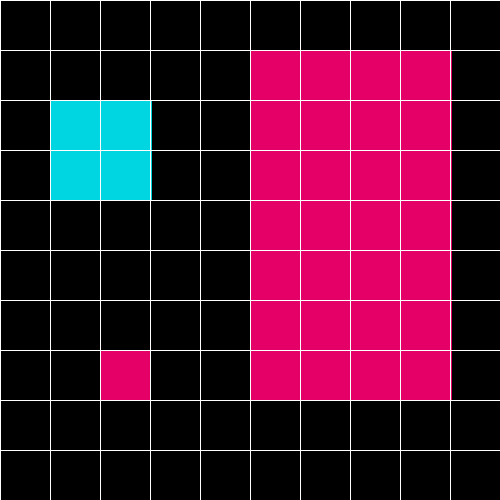
\includegraphics[width=\textwidth]{images/saf/ex_f_reg_seg}
		 \caption{Segmentation erronée : l'un des superpixels de \modif{la} classe noire a été attribué par erreur à la classe rose. Les contours des superpixels sont tracés en blanc.}
	\end{subfigure}	
	\caption{Distinction entre classes rares et erreurs de segmentation.}
	\label{fig:saf:classesRares}
\end{figure}

Soit $\mathbf{s}_{i}$ un superpixel, $x_{i}$ le sommet qui lui est associé et \modif{$\mathcal{P}= \lbrace P(\lambda_{1}|x_{i} ), \cdots, P(\lambda_{N_{\Lambda}}|x_{i} )  \rbrace$} l'ensemble des probabilités que ce superpixel appartienne à chacune des classes. La classe de \modif{label} $\lambda_{j}$ est attribuée à $x_{i}$ de manière à ce que :
\begin{equation}
P(\lambda_{j}|x_{i} )  \geqslant  P(\lambda_{k} | x_{i})\  \forall  k \in [1,N_{\Lambda}] \text{.}
\end{equation}
Après avoir ainsi obtenu une première segmentation, la probabilité $P_{i}(j)$ s'obtient rapidement en calculant l'histogramme normalisé des classes des superpixels voisins d'un superpixel de label $\lambda_{i}$. Soulignons que, du fait qu'une distribution de probabilité soit calculée pour chacune des classes $P_{i}(j) \neq P_{j}(i)$. Comme les arêtes de $\mathcal{G}$ sont non orientées, $P_{i}(j)$ et $P_{j}(i)$ \modif{doivent être fusionnées}. Nos tests ont montré que :
\begin{equation}
\mathcal{F}_{R}(x_{i},c_{i},x_{j},c_{j})= 1-\max(P_{i}(j),P_{j}(i))
\end{equation}
donne de bons résultats. \modif{L'utilisation de la fonction moyenne ou de la fonction minimum, à la place de la fonction maximum, ne permet pas d'améliorer la qualité des segmentations produites par $S \alpha F$}.

\subsection{Fonction de pondération}
La fonction de pondération $\omega$ dose l'influence du terme de régularisation par rapport au terme d'attache aux données. Dans la fonction \modif{de coût} définie par l'équation \ref{eq:safe:mrfprob}, le terme d'attache aux données intervient une fois par sommet, tandis que le terme de régularisation contribue à augmenter \modif{la valeur de la fonction} pour chaque arête, c'est-à-dire pour chaque couple de \modif{sommets} voisins. \modif{Pour que la contribution de la somme des termes de régularisation rattachés à un même sommet soit similaire quel que soit le nombre de voisin d'un sommet, il est} nécessaire que la fonction de pondération intègre \modif{le nombre de voisins de ce sommet. Soit $\nei(x_{i})$, la fonction renvoyant l'ensemble des sommets voisins de $x_{i}$.} Plusieurs tests nous ont conduit à sélectionner la fonction suivante :
\modif{
\begin{equation}
\omega (x_{i}) = \frac{\nombre{0,7}}{|\nei(x_{i})|}\text{.}
\end{equation}
}

\subsection{Algorithme $S \alpha F$ }

L'objectif de l'algorithme $S \alpha F$ consiste à minimiser la fonction $\mathcal{F}_{CAM}$. La figure \ref{fig:saf:algo} en schématise le fonctionnement général. 

L'approche $S \alpha F$ comprend une étape d'\emph{initialisation}, qui permet d'extraire les \modif{superpixels}, et une étape de \emph{segmentation}, où les germes donnés par l'utilisateur sont pris en compte. Tandis que l'étape d'initialisation ne nécessite d'être réalisée qu'une seule fois, l'étape de segmentation est répétée tant que l'utilisateur modifie les germes. 

Lors de l'étape d'initialisation, les pixels sont d'abord groupés en superpixels. Les \modif{caractéristiques} de chaque superpixel sont ensuite analysées et un descripteur sous la forme d'un vecteur à $N_{d}$ dimensions est calculé. Ainsi\modif{,} le nombre de primitives visuelles se voit considérablement réduit, chaque superpixel regroupant plusieurs centaines de pixels, ce qui accèlere les traitements effectués lors de l'étape de segmentation. 

Cette dernière concerne la minimisation à proprement parler de $\mathcal{F}_{CAM}$ et se déroule de la manière suivante :

\begin{enumerate}
\item les germes donnés par l'utilisateur sont analysés afin d'obtenir :
\begin{enumerate}
\item le nombre de classes $N_{\Lambda}$ ;
\item pour chaque classe, l'ensemble \modif{$\mathcal{S}_{A}^{\lambda_{i}}$ des superpixels nécessaires} pour entraîner la méthode de classification à reconnaître les superpixels appartenant à cette classe ;
\end{enumerate}
\item à l'aide de la méthode de classification, la probabilité de chaque superpixel d'appartenir à chacune des classes est calculée ;
\item l'obtention de ces probabilités permet de calculer\modif{,} pour chaque superpixel, le terme d'attache aux données \modif{$\mathcal{F}_{D}$} ;
\item une première segmentation est produite en attribuant à chaque superpixel la classe la plus probable ;
\item cette segmentation est analysée afin d'obtenir pour chaque couple de classes $(\lambda_{i}, \lambda_{j})$ les probabilités \modif{$P_{i}(j)$ et $P_{j}(i)$} ;
\item l'obtention de ces probabilités permet de calculer pour chaque paire de superpixels voisins le terme de régularisation \modif{$\mathcal{F}_{R}$} ;
\item une approximation de la segmentation correspondant à la valeur minimale de \modif{$\mathcal{F}_{CAM}$} est recherchée ;
\item le label attribué à chaque superpixel est transféré à l'ensemble des pixels le constituant ;
\item la segmentation résultat est montrée à l'utilisateur qui peut éventuellement ajouter ou supprimer des germes. 
\end{enumerate}

\begin{figure}[htbp]
\begin{center}
\scalebox{.5}{
\input{images/saf/algoOverview.pdf_t}
}
\caption{Schéma général de l'algorithme $S \alpha F$.}
\label{fig:saf:algo}
\end{center}
\end{figure}

À partir de cet algorithme général, toute une famille de méthodes peuvent être obtenues, dont les variations tiennent dans le choix de la méthode de sur-segmentation, des \modif{caractéristiques utilisées} pour décrire chaque superpixel, de la méthode de classification par apprentissage supervisé et de l'algorithme d'optimisation permettant de minimiser la fonction \modif{de coût}.

\section{Algorithme de sur-segmentation}

\subsection{Problématique}
L'algorithme de sur-segmentation utilisé doit permettre de regrouper rapidement les pixels de l'image en superpixels, de manière à minimiser la probabilité qu'un superpixel chevauche deux objets différents. L'obtention des superpixels ainsi que le \modif{calcul} de leurs descripteurs n'est réalisé qu'une seule fois, lors de l'étape d'initialisation. Comme la même classe est attribuée à l'ensemble de ses pixels, un superpixel contenant des pixels appartenant à deux éléments que l'utilisateur souhaite séparer engendrera des erreurs dans la segmentation résultat. \modif{Quel que} soit le nombre de germes ajoutés par l'utilisateur, cette erreur ne pourra pas être corrigée, puisqu'aucun mécanisme ne permet de séparer le superpixel en deux nouveaux superpixels. 

Le choix d'un algorithme de sur-segmentation est donc une étape clé pour le bon fonctionnement de $S \alpha F$. Suite à une \modif{évaluation des principales méthodes} existantes (qui fait l'objet du \modif{chapitre 4}), nous avons choisi l'algorithme SLIC (\og \textit{Simple Linear Iterative Clustering} \fg) \cite{achanta2012slic} qui fournit un bon compromis entre qualité du résultat et rapidité.

\subsection{Principe général de l'algorithme \modif{SLIC} et choix des paramètres} 

Proposé par Achanta \textit{et al.}  SLIC \cite{achanta2012slic}, est \modif{une} version modifiée de l'algorithme de $k$-moyennes. Des superpixels initiaux sont produits en regroupant les pixels selon une grille régulière. Le choix de taille des cases est un paramètre qu'il convient de fixer, soit en précisant un nombre souhaité de superpixels (les pixels de l'image sont alors découpés en autant de case que nécessaire), soit en précisant l'aire moyenne désirée pour les superpixels (la hauteur et la largeur des cases sont alors \modif{déterminées} pour s'approcher le plus possible de cette aire). 

L'algorithme SLIC répète alors une dizaine de fois les  deux étapes suivantes :
\begin{enumerate}
\item la couleur et la localisation \modif{moyennes} de chaque superpixel sont calculées ;
\item chaque pixel est rattaché au superpixel maximisant une fonction de similarité.
\end{enumerate}

L'une des contributions essentielles d'Achanta \textit{et al.} concerne la fonction permettant de mesurer la similarité entre un pixel et un superpixel. Cette dernière fait intervenir à la fois la couleur et la localisation. Un paramètre, fixé par l'utilisateur, permet de pondérer l'influence de chacune de ces deux informations.  

Une dernière étape permet d'uniformiser la taille des superpixels et de s'assurer que ces derniers correspondent bien à des composantes connexes.

Les deux paramètres \modif{à fixer} pour cette méthode sont donc \modif{:}
\begin{itemize}
\item le nombre de \modif{superpixels}, que nous avons fixé à $3000$\modif{, afin d'obtenir des superpixels suffisamment petits pour réduire les erreurs dans la sur-segmentation} ;
\item le poids pour la fonction de similarité, pour lequel Achanta \textit{et al.} \cite{achanta2012slic} recommandent une valeur de $10$\modif{,} ce qui s'est avéré pertinent dans le cas de $S \alpha F$.
\end{itemize}

Une description détaillée de l'algorithme SLIC est donnée \modif{dans la section} \ref{subsec:sp:slic}. La section \ref{subsec:sp:res-slic} contient, \modif{quant à} elle, une analyse des qualités nous ayant conduit à le choisir. 

\section{Description des superpixels }

\subsection{Problématique}

Les superpixels correspondant à des ensembles homogènes de pixels connexes, les descripteurs qui caractérisent leur apparence peuvent au choix, soit tirer partie de la diversité de l'information contenue dans un superpixel, soit chercher à la résumer. Les descripteurs de la première catégorie comprennent par exemple :
\begin{itemize}
\item les histogrammes \modif{des} différents canaux de \modif{couleur} ;
\item \modif{l'histogramme} d'un descripteur de texture tel que les textons ou les motifs binaires locaux \cite{pietikainen2011local} (LBP, de l'anglais \modif{\og \emph{Local Binary Patterns} \fg}).
\end{itemize}

Pour la seconde catégorie, nous trouvons\modif{,} entre autres :
\begin{itemize}
\item la moyenne \modif{de} chaque canal de couleur  ; 
\item l'écart type \modif{de} chaque canal de couleur  ;
\item le coefficient de dissymétrie  \modif{de} chaque canal de couleur ; 
\item le kurtosis \modif{de} chaque canal de couleur  ; 
\item la position du barycentre ;
\item l'aire en nombre de pixels ;
\item le rapport entre l'aire \modif{du superpixel} et celle du plus petit rectangle l'englobant. 
\end{itemize}

Les descripteurs choisis doivent permettre de regrouper les superpixels appartenant à la même classe, tout en séparant ceux \modif{correspondant} à des objets différents. \modif{Ne disposant d'aucune connaissance \textit{a priori} sur l'image}, ni sur les propriétés de la segmentation que l'utilisateur voudra obtenir, ils doivent également s'adapter à un large panel de situations. Enfin, ni leur extraction durant l'étape \modif{d'initialisation, }ni leur utilisation durant l'étape de segmentation ne doivent se répercuter de manière trop importante sur les temps d'exécution. 

Certaines caractéristiques, notamment celles associées à la texture, requièrent un nombre de calculs élevé lors de l'étape d'initialisation. Par ailleurs, plus le descripteur contient de caractéristiques, plus le temps nécessaire \modif{pour évaluer} la probabilité d'un superpixel d'appartenir à chacune des classes est important. 

\subsection{Choix d'un descripteur}

Nous avons choisi un descripteur \modif{minimaliste} comprenant cinq caractéristiques :
\begin{itemize}
\item trois pour exprimer la couleur moyenne du superpixel dans l'espace colorimétrique RGB ;
\item deux pour exprimer sa localisation dans l'image, \modif{par} les coordonnées de son barycentre.
\end{itemize} 

Ces cinq caractéristiques sont normalisées : pour la couleur, nous divisons chaque moyenne par $255$ \modif{;} pour les coordonnées du barycentre\modif{,} nous divisions l'abscisse par la largeur de l'image et l'ordonnée par la hauteur de l'image. Nous obtenons un descripteur rapide à calculer lors de la phase d'initialisation et comprenant peu de caractéristiques, ce qui accélère son utilisation lors de l'étape de segmentation.  

L'information de couleur permet de segmenter rapidement et avec un minimum de germes de larges zones homogènes telles que le ciel. Lorsque l'utilisateur souhaite séparer deux objets ayant des teintes similaires, l'information de localisation prend le relais. Cette dernière assure également que les germes conservent un comportement local c'est-à-dire que l'ajout de germes sur une partie de l'image ne perturbe pas la segmentation dans le reste de la photographie.


\begin{emodif}
\subsection{Problèmes liés au positionnement des germes}
\label{subsec:eval:posgermes}

En contrepartie des deux qualités de ce descripteur -- sa rapidité et l'influence intuitive des germes -- la simplicité de ce dernier fait que, dans certains cas, les indications données par l'utilisateur peuvent ne pas être suffisantes pour trouver une segmentation pertinente de l'image. 

Tout d'abord, les germes peuvent ne pas être suffisants pour créer un modèle des objets à extraire pertinent en termes de couleur. Un exemple est présenté sur la figure \ref{fig:eval:Algo-fails-c}. Le pollen de cette dernière, en jaune, n'est pas correctement segmenté. Aucun pixel jaune n'étant sélectionné comme germe, cette teinte est rattachée à tort au fond, dont la couleur verte est plus proche du jaune que du rouge des pétales de la fleur. L'ajout de quelques germes sur l'une des deux zones centrales des fleurs suffit à améliorer netteent la qualité de la segmentation. 
 
\begin{figure}[htb]
 \centering
 \begin{subfigure}{0.4\textwidth}	
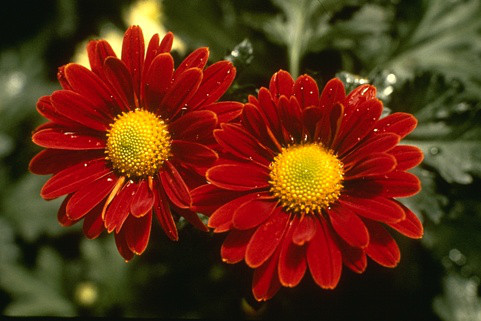
\includegraphics[width=\textwidth]{images/evaluation/fails/im_c}
 \end{subfigure}
 \\~\\
 \begin{subfigure}{0.4\textwidth}	
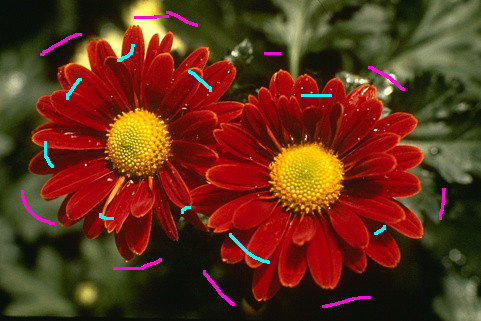
\includegraphics[width=\textwidth]{images/evaluation/fails/germes_c_01}
 \end{subfigure}
 ~
 \begin{subfigure}{0.4\textwidth}	

\includegraphics[width=\textwidth]{images/evaluation/fails/seg_c_01}
 \end{subfigure}
 \\~\\
 \begin{subfigure}{0.4\textwidth}	
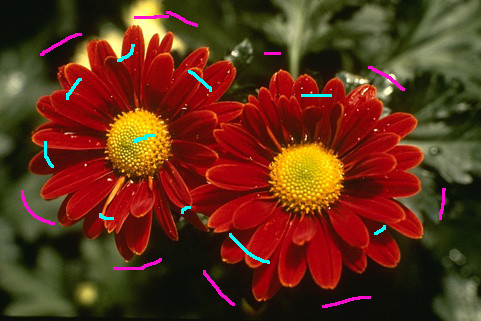
\includegraphics[width=\textwidth]{images/evaluation/fails/germes_c_02}
 \end{subfigure}
 ~
 \begin{subfigure}{0.4\textwidth}	

\includegraphics[width=\textwidth]{images/evaluation/fails/seg_c_02}
 \end{subfigure}
\caption{Illustration de l'impact de la répartition des germes en termes de couleur  sur la qualité de la segmentation obtenue.}
	\label{fig:eval:Algo-fails-c}
\end{figure} 

Inversement, les germes peuvent ne pas être répartis correctement dans l'image en termes de localisation, à l'instar de l'exemple donné sur la figure \ref{fig:eval:Algo-fails}. Ici, même si théoriquement la couleur devrait permettre de séparer correctement l'éléphant, le ciel et la végétation, l'utilisation d'une information de localisation vient perturber la méthode de classification pour la partie gauche de l'image qui, contrairement à la moitié droite, ne contient pas de germes. 

\begin{figure}[htb]
 \centering
 \begin{subfigure}{0.4\textwidth}	
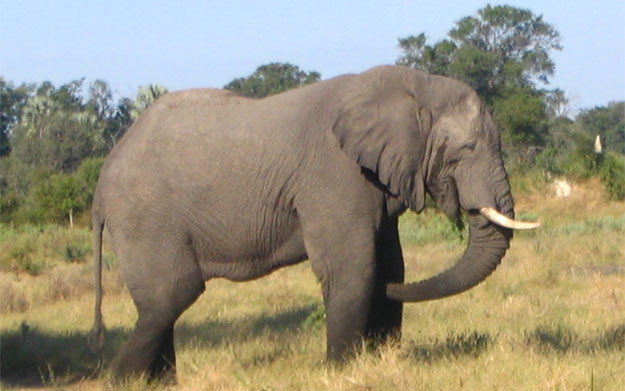
\includegraphics[width=\textwidth]{images/evaluation/fails/im}
 \end{subfigure}
 \\~\\
 \begin{subfigure}{0.4\textwidth}	
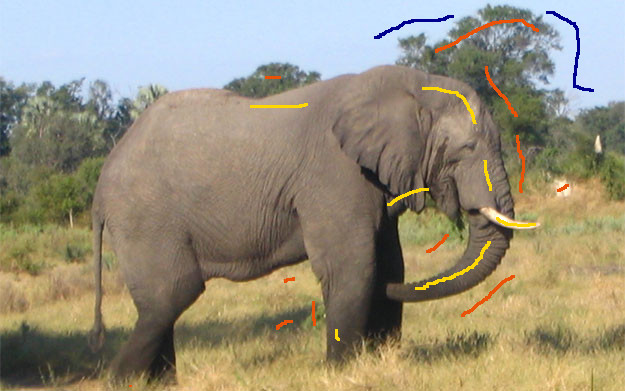
\includegraphics[width=\textwidth]{images/evaluation/fails/germes_01}
 \end{subfigure}
 ~
 \begin{subfigure}{0.4\textwidth}	

\includegraphics[width=\textwidth]{images/evaluation/fails/seg_01}
 \end{subfigure}
 \\~\\
 \begin{subfigure}{0.4\textwidth}	
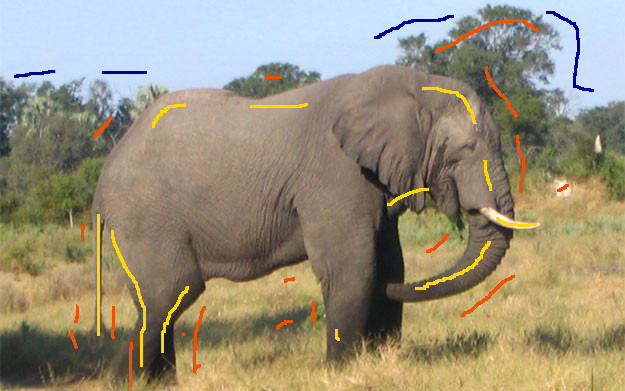
\includegraphics[width=\textwidth]{images/evaluation/fails/germes_02}
 \end{subfigure}
 ~
 \begin{subfigure}{0.4\textwidth}	

\includegraphics[width=\textwidth]{images/evaluation/fails/seg_02}
 \end{subfigure}
\caption{Illustration de l'impact de la répartition des germes \modif{en termes de localisation} sur la qualité de la segmentation obtenue.}
	\label{fig:eval:Algo-fails}
\end{figure} 

Afin d'éviter ce dernier problème, une consigne simple peut être donnée à l'utilisateur lui demandant de donner des germes \og \textit{près des contours}\fg. 

\end{emodif}

\subsection{Autres descripteurs testés }

En remplaçant  l'espace RGB par d'autres espaces colorimétriques (CIELab, HSV) nous n'avons pas constaté d'améliorations significatives. 

Il en va de même avec l'utilisation d'un descripteur de texture, dont le coût en termes de temps de calcul n'est pas compensé par une amélioration notable des performances (réduction du nombre de germes nécessaires et/ou diminution des erreurs dans la segmentation). Ainsi, nos tests avec les LBP, descripteur de texture pourtant à l'origine d'avancées notables dans de nombreux travaux en vision par ordinateur, ne nous ont pas permis d'améliorer les scores de précision de notre méthode.

L'utilisation des histogrammes de LBP s'est en revanche traduite par une augmentation du temps d'exécution de $23\%$ pour l'étape d'initialisation et de $76\%$ pour l'étape de segmentation. Ce résultat n'est  pas surprenant : les superpixels sont conçus sur la base de la couleur des pixels, de manière à former des ensembles homogènes. Ainsi, l'écart type moyen pour l'ensemble des données que nous avons utilisées ne dépasse pas les $4\%$, ce qui indique que les pixels au sein d'un même superpixel présentent peu de variations en termes de couleur.


\section{Choix d'une méthode de classification supervisée}
\label{sec:saf:SelectClassifSup}

L'approche de Wu \textit{et al.} \cite{wu2004probability}  est connue pour donner de bons résultats à la fois avec les méthodes de classification  SVM et  FA. Le choix de l'une de ces méthodes pour estimer la  probabilité qu'un superpixel appartienne à une classe, nécessite de s'intéresser aux forces et aux faiblesses de chacune d'entre elles, dans le cadre spécifique du problème de la segmentation interactive tel que nous l'avons posé. 

Ainsi, par rapport aux problèmes de classification par apprentissage canoniques, nous pouvons noter les particularités suivantes :
\begin{itemize}
\item nous disposons de peu de données d’apprentissage ;
\item de nombreuses images présentent des classes \emph{rares} ;
\item le descripteur  de chaque superpixel comprend peu de caractéristiques. 
\end{itemize}

Les données d'apprentissage étant spécifiques à une image, elles correspondent à un sous-ensemble des superpixels produits. Or, pour conserver des temps d'exécution raisonnables, le nombre de ces derniers ne doit pas dépasser \modif{ quelques milliers}. Si nous estimons que l'utilisateur annote environ $25 \%$ des superpixels, ce qui correspond déjà à un nombre élevé de germes et à un effort conséquent pour guider la méthode, nous disposons \modif{de} seulement quelques centaines de données d'apprentissage, à répartir entre les différentes classes. 

Parmi ces classes, certaines correspondent à de petits objets dont la surface en nombre de pixels est très inférieure à celles des autres composantes de l'image. \modif{Il est donc }probable que les données d'apprentissage pour ces classes soit moins nombreuses (quelques dizaines de superpixels).

Le fait que les descripteurs utilisés ne contiennent que cinq caractéristiques constitue également une singularité, de nombreux problèmes de classification ayant plutôt à faire face à un descripteur de taille trop importante, qu'il convient de réduire\modif{,} par exemple avec une analyse en composantes principales.

À ces spécificités inhérentes au contexte applicatif de la segmentation interactive, s'ajoutent celles liées à l'utilisation de la	 méthode de classification au sein de $S \alpha F$ et qui consiste à :
\begin{itemize}
\item estimer pour chaque superpixel une distribution de probabilité permettant de calculer le terme d'attache aux données ;
\item produire une segmentation initiale dont dépend la pertinence du terme de régularisation.
\end{itemize}

Le dernier point est sans doute le plus simple à évaluer : sachant la classe réelle d'un superpixel, il suffit de vérifier qu'elle correspond à sa classe prédite. Vérifier la qualité de la distribution de probabilité est plus \modif{délicat}. À partir de données de référence où chaque pixel est attribué à une classe, nous avons cherché à produire un nouvel ensemble de données de référence associant à chaque superpixel une distribution de probabilité de référence. Cela nous permet notamment de prendre en compte le fait qu'un superpixel en bordure d'un objet puisse avoir des caractéristiques proches de celles de plusieurs classes : dans ce cas de figure, nous préférons obtenir une distribution de probabilité témoignant de cette incertitude qu'une prédiction assurée pour l'une ou l'autre des classes. 

Enfin, soulignons que nos tests ont été réalisés à l'échelle du superpixel et non du pixel. En effet, un pixel se voit attribuer la classe du superpixel auquel il appartient. Les sources d'erreurs dans la segmentation présentes à cette échelle peuvent donc provenir soit d'une distribution de probabilité erronnée, soit d'une erreur commise par la méthode de sur-segmentation employée. Ici, seul le premier cas de figure nous intéresse. 

\subsection{Fonctionnement des deux méthodes}
\subsubsection{Séparateur à vaste marge}

Le principe \modif{d'un} SVM est illustré par la figure \ref{fig:saf:svm}. Il consiste à représenter une donnée comme un point dans un espace à $N_{D}$ dimensions et à lui attribuer une classe en fonction de sa position par rapport à un hyperplan. Pour déterminer la position de l’hyperplan, le classificateur SVM réalise une étape d’apprentissage durant laquelle il dispose de données déjà classées et cherche l’équation d’un hyperplan séparant les deux ensembles de points, de manière à maximiser l’écart $b$ entre les points périphériques (les vecteurs de support) et cet hyperplan de séparation. Si nous considérons nos données comme des vecteurs de $N_{d}$ éléments, un cas idéal serait celui où $N_{d} = N_{D}$. Concrètement, pour trouver un hyperplan séparant toutes les données, $N_{D}$ s’avère généralement très supérieur à $N_{d}$.

Il n’est pas toujours souhaitable que l’hyperplan sépare parfaitement l’ensemble des points : des points mal classés durant la phase d’apprentissage peuvent être tolérés afin de garantir qu’une marge entre les \modif{vecteurs de support} soit plus importante. Par exemple, dans le cas de la segmentation interactive, il est possible que l’utilisateur ait légèrement débordé lors de son tracé du germe, et qu’ainsi un superpixel soit attribué à tort à une classe. Il est intéressant que ces données d’apprentissage erronées puissent ne pas être prise en considération. Un paramètre  $\omega_{C}$ permet de pondérer l’importance des erreurs de classification par rapport
à celle de la largeur de la marge.


\begin{figure}[htb]
\begin{center}
\scalebox{.5}{
\input{images/saf/svm.pdf_t}
}
\caption{L’hyperplan optimal (en rouge), caractérisé par le vecteur $w$, avec la marge maximale $b$.
Les échantillons entourés en vert sont des \modif{vecteurs de support}. Les échantillons entourés en rouge sont des
erreurs tolérées lors de la phase d’apprentissage.}
\label{fig:saf:svm}
\end{center}
\end{figure}

L’évaluation de la distance entre deux points, dans un espace à $N_{D}$ dimensions, est réalisé au moyen d’une fonction nommée noyau. Pour le problème de segmentation interactive que nous cherchons à résoudre, nous avons utilisé le noyau \modif{RBF, de l'anglais \og \emph{Radial Basis Function}\fg} :
\begin{equation}
K_{RBF}(u,v) = \exp(- \omega_{\Phi} ||u-v||^{2}) 
\end{equation}
avec $u$ et $v$ les données dont nous voulons évaluer la distance et $\omega_{\Phi}$ un paramètre du noyau. Les tests que nous avons menés avec d'autres noyaux n'ont pas permis une amélioration significative des résultats. 


\subsubsection{Forêt Aléatoire}
Le principe des FA ayant déjà fait l'objet d'une présentation détaillée à la section \ref{sec:sota:santner}, nous nous contenterons de rappeler ici les quelques points fondamentaux qui permettent de comprendre les résultats de notre évaluation :
\begin{itemize}
\item une FA correspond à un ensemble d'arbres de décision ;
\item chaque arbre est entraîné séparément, avec un sous-ensemble des données d'apprentissage ;
\item chaque arbre est spécialisé sur un petit nombre de caractéristiques, inférieur à la taille du descripteur ;
\item lorsqu'une nouvelle donnée doit être classée, l'ensemble des arbres \modif{votent} : la classe ayant obtenu le maximum de votes est attribuée à la donnée. 
\end{itemize}



\subsection{Protocole expérimental}
Afin de comparer les deux méthodes de classification supervisée, nous avons utilisé, d'une part, l'implémentation d'une FA de la bibliothèque  Alglib  \footnote{\url{www.alglib.net}} et, d'autre part, l'implémentation C-SVM, contenue dans la bibliothèque  libSVM \footnote{\url{www.csie.ntu.edu.tw/~cjlin/libsvm}}. Chacune des deux implémentations nécessite deux  paramètres : 
\begin{itemize}
\item le paramètre du noyau\modif{,} $\omega_{\Phi}$, et le paramètre \modif{de prise en compte des erreurs dans les données d'apprentissage,} $\omega_{C}$ dans le cas du SVM ;
\item  le nombre d'arbres de décision et  le pourcentage de données d'apprentissage utilisées pour entraîner chaque arbre de décision dans le cas de la FA.
\end{itemize}

 Nous nous sommes intéressés à l'évolution des performances de ces deux méthodes en fonction des couples de \modif{paramètres.} Les trois critères quantitatifs que nous avons employés sont les suivants :
\begin{itemize}
\item l'adéquation entre les probabilités produites et la réalité, donnée par le taux d'erreur $\mathcal{F}_{Err}$;
\item le temps d'exécution moyen pour \modif{l’entraînement} de la méthode ;
\item le temps d'exécution moyen nécessaire pour estimer les probabilités pour l'ensemble des classes et des superpixels, une fois que l'apprentissage est réalisé. Par la suite, nous parlerons de temps d'exécution pour la \emph{phase d'exploitation}.
\end{itemize}

Soit un ensemble de données de référence composé de couples $(I,R)$ associant à une image une segmentation de référence $R$ où chaque pixel est attribué à une unique classe. L'image $I$ est sur-segmentée en $N_{\mathbb{S}}$ superpixels, dont les \modif{caractéristiques} sont extraites afin d'obtenir un ensemble de variables \modif{$X=\lbrace x_{1}, \cdots, x_{N_{\mathbb{S}} } \rbrace$} semblable à celui utilisé par $S \alpha F$. Pour chaque variable $x_{i}$, une estimation de la probabilité $P_{R}(\lambda_{j} | x_{i})$ est obtenue en calculant \modif{la proportion} de pixels rattachés à $x_{i}$ et attribués à la classe de label $\lambda_{j}$ dans $R$. En estimant $P_{R}(\lambda_{j} | x_{i})$ pour l'ensemble des classes présentes dans la vérité terrain, nous obtenons \modif{$\mathcal{P}_{R}$} la distribution de probabilité de référence du superpixel. Soit \modif{$\mathcal{P}_{classif}$} la distribution de probabilité estimée à l'aide le l'approche de Wu \textit{et al.} \cite{wu2004probability} : 
\modif{\begin{equation}
\mathcal{F}_{Err}(\modif{P}_{R},\modif{P}_{classif}) = \sum_{i=1}^{N_{I}} \sqrt{ \sum_{j=1}^{N_{\Lambda}}  (P_{classif}(\lambda_{j}| x_{i}) - P_{R}(\lambda_{j}| x_{i}))^{2}}\text{.}
\end{equation}}

Les performances des deux méthodes\modif{,} SVM et FA\modif{,} ont été analysées sur la base de \modif{deux} ensembles de données de référence : celui de Santner \textit{et al.} \cite{santner2010interactive} et celui de McGuinness \textit{et al.}~\cite{mcguinness2010comparative}. Afin de ne pas sur-apprendre les paramètres de chacune des méthodes et de ne pas biaiser les résultats de l'évaluation de $S \alpha F$ qui utilise également ces \modif{données de référence}, nous nous sommes contentés de prélever un tiers des segmentations de \modif{référence}, soit $100$ images pour Santner \textit{et al.} \cite{santner2010interactive}  et $34$ images pour McGuinness \textit{et al.} \cite{mcguinness2010comparative}. Par la suite, nous désignerons ces deux ensembles respectivement par $R^{ MC}$ et $R^{ BI}$. Le premier correspond à des problèmes de segmentation interactive \modif{multiclasse} ($MC$), tandis que le second ne contient que des \modif{binarisations ($BI$)}.

La figure \ref{fig:saf:stnerClasses} donne la répartition du nombre de classes pour $R^{ MC}$. Celui-ci varie de $2$ à $7$, avec une majorité de segmentations comprenant $2$ et $4$ classes. 
\begin{figure}[htb]
\begin{center}
\scalebox{.5}{
\input{images/saf/santernClasses.pdf_t}
}
\caption{Répartition du nombre de classes pour l'ensemble de \modif{données de référence} $R^{ MC}$.}
\label{fig:saf:stnerClasses}
\end{center}
\end{figure}

Les temps d'exécution ont été obtenus sur un ordinateur de bureau, équipé d'un processeur \emph{Intel Core i7} \modif{$\nombre{2,6}$} GHz et d'une RAM de 16 Go. \modif{L'adéquation entre les probabilités estimées par une méthode et la réalité est calculée en faisant la moyenne du score $\mathcal{F}_{Err}$ obtenu pour tous les superpixels, de toutes les images d'un ensemble de données.}

Les trois mesures sont calculées pour chaque couple de paramètres de chaque méthode, soit $256$ tests pour le SVM et $100$ tests pour la FA. Il n'est donc pas envisageable de mettre en place un protocole où un utilisateur donnerait les germes nécessaires à l'apprentissage de chacune des $356$ variantes. Nous avons choisi d'automatiser la sélection des données d'apprentissage \modif{de la manière suivante} :
\begin{enumerate}
\item pour chaque classe $\lambda_{i}$, nous créons un ensemble de données, constitué des superpixels $x_{j}$ tels que $P_{R}(\lambda_{i} | x_{j}) > P_{R}(\lambda_{k} | x_{j}) \ \forall k \neq i$\modif{, c'est-à-dire ceux pour lesquels la classe la plus probable dans les données de référence est $\lambda_{i}$} ;
\item nous classons les $N_{\lambda_{i}}$ superpixels de cet ensemble par ordre d'apparition dans l'image, du haut vers le bas et de la gauche vers la droite ;
\item \modif{dans cet ensemble de superpixels classés}, nous sélectionnons comme données d'apprentissage $N_{app}$ superpixels, en laissant un écart constant de \modif{$N_{step}=\dfrac{N_{app}}{N_{\lambda_{i}}} -1$} superpixels entre chaque paire de superpixels prélevés consécutivement.
\end{enumerate}
Nous obtenons ainsi un ensemble de données d'apprentissage réparties uniformément (en termes de localisation) dans l'image. Nous avons fait des tests avec différentes valeurs pour $N_{app}$. Les résultats que nous analyserons dans ce chapitre correspondent à $N_{app}=100$\modif{.} Les tendances demeurent les même en augmentant $N_{app}$.

\subsection{Résultats \modif{avec} \modif{le séparateur à vaste marge}}
Les tableaux \ref{tab:saf:mvs_mc_precision} et \ref{tab:saf:mvs_bi_precision} donnent l'évolution du taux d'erreur $\mathcal{F}_{err}$ pour la méthode de classification SVM, par rapport aux données de \modif{référence} $R^{MC}$ et  $R^{BI}$.  L'analyse de ces résultats montre que pour le couple de paramètre $(\omega_{C},\omega_{\Phi})$, un grand nombre de valeurs  garantit un taux d'erreur inférieur à $5 \%$. Ces valeurs forment un large palier et indiquent que le choix des paramètres $\omega_{C}$ et $\omega_{\phi}$ n'est pas critique par rapport aux performances de la méthode SVM. Nous avons donc de bonnes raisons de penser qu'il n'y aura pas lieu de les modifier pour les adapter à d'autres jeux de données. 

Pour les données de référence de $R^{MC}$, le taux d'erreur minimum est de $4 \%$.  Dans le cas des images de $R^{BI}$  il descend autour de $1\%$. Les distributions de \modif{probabilité estimées} semblent plus fidèles pour les images de $R^{BI}$, avec un taux d'erreur moins élevé. Ce résultat pourrait s'expliquer par le fait que la classification par SVM concerne, à l'origine, des problèmes à deux classes. L'extension à des problèmes multiclasses constitue, au moins dans le cadre de nos tests, une difficulté supplémentaire. 

Les tableaux \ref{tab:saf:mvs_mc_t_training} et \ref{tab:saf:mvs_bi_t_training} contiennent les résultats concernant l'évolution du temps d'exécution lors de la phase d'entraînement. Ils montrent que lorsque le SVM est correctement \modif{paramétré}, le temps nécessaire pour trouver les vecteurs de support diminue. Nous ne constatons pas de différence notable entre les deux ensembles de données.

Enfin\modif{,} les tableaux \ref{tab:saf:mvs_mc_t_exp} et \ref{tab:saf:mvs_bi_t_exp} présentent les temps d'exécution lors de la phase d'exploitation. Nous pouvons en tirer les mêmes conclusions que pour la phase d'apprentissage, en constatant que\modif{,} lorsqu'elle est correctement paramétrée\modif{,} la méthode produit plus rapidement les distributions de probabilité des superpixels.

%gris
\begin{table}[htb]
\caption{Taux d'erreur (exprimé\modif{s} en pourcentage\modif{s}) de la méthode SVM obtenus avec les données $R^{MC}$. Les valeurs sur la première ligne correspondent au paramètre $\omega_{C}$, ceux sur la première colonne au paramètre $\omega_{\Phi}$.}
\centering
\begin{tabular}{| p{0.5cm} | p{0.5cm} |p{0.5cm} |p{0.5cm} |p{0.5cm} |p{0.5cm} |p{0.5cm} |p{0.5cm} |p{0.5cm} |p{0.5cm} |p{0.5cm} |p{0.5cm} |p{0.5cm} |p{0.5cm} |p{0.5cm} |p{0.5cm} |p{0.5cm} |}
\hline
& $\cellcolor{gris}{2^{-6}}$&$\cellcolor{gris}{2^{-5}}$&$\cellcolor{gris}{2^{-4}}$&$\cellcolor{gris}{2^{-3}}$&$\cellcolor{gris}{2^{-2}}$&$\cellcolor{gris}{2^{-1}}$&$\cellcolor{gris}{1}$&$\cellcolor{gris}{2}$&$\cellcolor{gris}{2^{2}}$&$\cellcolor{gris}{2^{3}}$&$\cellcolor{gris}{2^{4}}$&$\cellcolor{gris}{2^{5}}$&$\cellcolor{gris}{2^{6}}$&$\cellcolor{gris}{2^{7}}$&$\cellcolor{gris}{2^{8}}$&$\cellcolor{gris}{2^{9}}$\\
\hline
\modif{$\cellcolor{gris}{2^{-6}}$}& $22$ & $22$ & $22$ & $22$ & $21$ & $18$ & $15$ & $13$ & $12$ & $11$ & $10$ & $10$ & $9$ & $8$ & $8$ & $6$ \\
\hline
$\cellcolor{gris}{2^{-5}}$ & $23$ & $22$ & $22$ & $21$ & $18$ & $15$ & $13$ & $12$ & $11$ & $10$ & $10$ & $9$ & $8$ & $7$ & $6$ & $5$ \\
\hline
$\cellcolor{gris}{2^{-4}}$ & $22$ & $22$ & $21$ & $18$ & $15$ & $13$ & $12$ & $11$ & $10$ & $9$ & $8$ & $7$ & $6$ & $5$ & $5$ & $4$ \\
\hline
$\cellcolor{gris}{2^{-3}}$ & $22$ & $21$ & $18$ & $15$ & $12$ & $11$ & $11$ & $10$ & $9$ & $7$ & $6$ & $5$ & $5$ & $4$ & $4$ & $4$ \\
\hline
$\cellcolor{gris}{2^{-2}}$ & $21$ & $18$ & $15$ & $13$ & $11$ & $10$ & $9$ & $8$ & $7$ & $6$ & $5$ & $4$ & $4$ & $4$ & $3$ & $3$ \\
\hline
$\cellcolor{gris}{2^{-1}}$ & $19$ & $15$ & $12$ & $11$ & $9$ & $8$ & $7$ & $6$ & $5$ & $4$ & $4$ & $4$ & $3$ & $3$ & $3$ & $3$ \\
\hline
$\cellcolor{gris}{1}$ & $16$ & $12$ & $10$ & $9$ & $7$ & $6$ & $5$ & $4$ & $4$ & $3$ & $3$ & $3$ & $3$ & $3$ & $3$ & $3$ \\
\hline
$\cellcolor{gris}{2}$ & $13$ & $10$ & $8$ & $7$ & $6$ & $5$ & $4$ & $4$ & $3$ & $3$ & $3$ & $3$ & $3$ & $3$ & $3$ & $3$ \\
\hline
$\cellcolor{gris}{2^2}$ & $13$ & $8$ & $6$ & $5$ & $4$ & $4$ & $3$ & $3$ & $3$ & $3$ & $3$ & $3$ & $3$ & $3$ & $3$ & $3$ \\
\hline
$\cellcolor{gris}{2^3}$ & $14$ & $7$ & $5$ & $4$ & $4$ & $3$ & $3$ & $3$ & $2$ & $2$ & $2$ & $2$ & $3$ & $3$ & $3$ & $3$ \\
\hline
$\cellcolor{gris}{2^4}$ & $16$ & $10$ & $5$ & $4$ & $3$ & $3$ & $3$ & $2$ & $2$ & $2$ & $2$ & $3$ & $3$ & $3$ & $3$ & $3$ \\
\hline
$\cellcolor{gris}{2^5}$ & $17$ & $15$ & $7$ & $3$ & $3$ & $3$ & $2$ & $2$ & $2$ & $2$ & $2$ & $3$ & $3$ & $3$ & $3$ & $3$ \\
\hline
$\cellcolor{gris}{2^6}$ & $19$ & $18$ & $14$ & $6$ & $3$ & $3$ & $3$ & $3$ & $3$ & $3$ & $3$ & $3$ & $3$ & $3$ & $3$ & $3$ \\
\hline
$\cellcolor{gris}{2^7}$ & $18$ & $18$ & $17$ & $13$ & $5$ & $3$ & $3$ & $3$ & $3$ & $3$ & $3$ & $3$ & $3$ & $3$ & $3$ & $3$ \\
\hline
$\cellcolor{gris}{2^8}$ & $20$ & $20$ & $19$ & $18$ & $13$ & $6$ & $4$ & $4$ & $4$ & $4$ & $4$ & $4$ & $4$ & $4$ & $4$ & $4$ \\
\hline
$\cellcolor{gris}{2^9}$ & $20$ & $20$ & $21$ & $20$ & $20$ & $14$ & $7$ & $7$ & $7$ & $7$ & $7$ & $7$ & $7$ & $7$ & $7$ & $7$ \\
\hline
\end{tabular}
\label{tab:saf:mvs_mc_precision}
\end{table}

\begin{table}[htb]
\caption{Taux d'erreur (exprimé\modif{s} en pourcentage\modif{s}) de la méthode SVM obtenus avec les données $R^{BI}$. Les valeurs sur la première ligne correspondent au paramètre $\omega_{C}$, ceux sur la première colonne au paramètre $\omega_{\Phi}$.}
\centering
\begin{tabular}{| p{0.5cm} | p{0.5cm} |p{0.5cm} |p{0.5cm} |p{0.5cm} |p{0.5cm} |p{0.5cm} |p{0.5cm} |p{0.5cm} |p{0.5cm} |p{0.5cm} |p{0.5cm} |p{0.5cm} |p{0.5cm} |p{0.5cm} |p{0.5cm} |p{0.5cm} |}
\hline
& $\cellcolor{gris}{2^{-6}}$&$\cellcolor{gris}{2^{-5}}$&$\cellcolor{gris}{2^{-4}}$&$\cellcolor{gris}{2^{-3}}$&$\cellcolor{gris}{2^{-2}}$&$\cellcolor{gris}{2^{-1}}$&$\cellcolor{gris}{1}$&$\cellcolor{gris}{2}$&$\cellcolor{gris}{2^{2}}$&$\cellcolor{gris}{2^{3}}$&$\cellcolor{gris}{2^{4}}$&$\cellcolor{gris}{2^{5}}$&$\cellcolor{gris}{2^{6}}$&$\cellcolor{gris}{2^{7}}$&$\cellcolor{gris}{2^{8}}$&$\cellcolor{gris}{2^{9}}$\\
\hline
$\cellcolor{gris}{2^{-6}}$ & $10$ & $11$ & $11$ & $10$ & $10$ & $10$ & $9$ & $8$ & $8$ & $8$ & $7$ & $7$ & $6$ & $6$ & $5$ & $4$ \\
\hline
$\cellcolor{gris}{2^{-5}}$ & $11$ & $11$ & $10$ & $10$ & $10$ & $9$ & $8$ & $8$ & $8$ & $7$ & $7$ & $6$ & $5$ & $4$ & $3$ & $3$ \\
\hline
$\cellcolor{gris}{2^{-4}}$ & $10$ & $11$ & $10$ & $9$ & $8$ & $8$ & $8$ & $8$ & $7$ & $6$ & $5$ & $4$ & $4$ & $3$ & $3$ & $2$ \\
\hline
$\cellcolor{gris}{2^{-3}}$ & $10$ & $9$ & $9$ & $8$ & $8$ & $8$ & $7$ & $7$ & $6$ & $5$ & $4$ & $3$ & $3$ & $2$ & $2$ & $2$ \\
\hline
$\cellcolor{gris}{2^{-2}}$ & $9$ & $9$ & $8$ & $8$ & $7$ & $7$ & $6$ & $5$ & $4$ & $3$ & $3$ & $2$ & $2$ & $2$ & $2$ & $2$ \\
\hline
$\cellcolor{gris}{2^{-1}}$ & $9$ & $8$ & $7$ & $7$ & $6$ & $5$ & $4$ & $3$ & $3$ & $2$ & $2$ & $2$ & $2$ & $2$ & $1$ & $1$ \\
\hline
$\cellcolor{gris}{1}$ & $8$ & $7$ & $6$ & $5$ & $4$ & $4$ & $3$ & $3$ & $2$ & $2$ & $2$ & $2$ & $1$ & $1$ & $1$ & $1$ \\
\hline
$\cellcolor{gris}{2}$ & $5$ & $5$ & $5$ & $4$ & $3$ & $3$ & $2$ & $2$ & $2$ & $2$ & $1$ & $1$ & $1$ & $1$ & $1$ & $1$ \\
\hline
$\cellcolor{gris}{2^2}$ & $4$ & $4$ & $4$ & $3$ & $3$ & $2$ & $2$ & $2$ & $1$ & $1$ & $1$ & $1$ & $1$ & $1$ & $1$ & $1$ \\
\hline
$\cellcolor{gris}{2^3}$ & $4$ & $3$ & $3$ & $2$ & $2$ & $2$ & $1$ & $1$ & $1$ & $1$ & $1$ & $1$ & $1$ & $1$ & $1$ & $1$ \\
\hline
$\cellcolor{gris}{2^4}$ & $4$ & $2$ & $2$ & $2$ & $2$ & $1$ & $1$ & $1$ & $1$ & $1$ & $1$ & $1$ & $1$ & $1$ & $1$ & $1$ \\
\hline
$\cellcolor{gris}{2^5}$ & $4$ & $4$ & $2$ & $2$ & $1$ & $1$ & $1$ & $1$ & $1$ & $1$ & $1$ & $1$ & $1$ & $1$ & $1$ & $1$ \\
\hline
$\cellcolor{gris}{2^6}$ & $5$ & $5$ & $3$ & $1$ & $1$ & $1$ & $1$ & $1$ & $1$ & $1$ & $1$ & $1$ & $1$ & $1$ & $1$ & $1$ \\
\hline
$\cellcolor{gris}{2^7}$ & $6$ & $7$ & $5$ & $3$ & $1$ & $1$ & $1$ & $1$ & $1$ & $1$ & $1$ & $1$ & $1$ & $1$ & $1$ & $1$ \\
\hline
$\cellcolor{gris}{2^8}$ & $7$ & $6$ & $6$ & $4$ & $3$ & $2$ & $2$ & $2$ & $2$ & $2$ & $2$ & $2$ & $2$ & $2$ & $2$ & $2$ \\
\hline
$\cellcolor{gris}{2^9}$ & $6$ & $7$ & $7$ & $7$ & $6$ & $4$ & $3$ & $3$ & $3$ & $3$ & $3$ & $3$ & $3$ & $3$ & $3$ & $3$ \\
\hline
\end{tabular}
\label{tab:saf:mvs_bi_precision}
\end{table}

\begin{table}[htb]
\caption{Temps d'exécution (en dixièmes de seconde) pour la phase d'entraînement de la méthode SVM obtenus avec les données $R^{MC}$. Les valeurs sur la première ligne correspondent au paramètre $\omega_{C}$, ceux sur la première colonne au paramètre $\omega_{\Phi}$.}
\centering
\begin{tabular}{| p{0.5cm} | p{0.5cm} |p{0.5cm} |p{0.5cm} |p{0.5cm} |p{0.5cm} |p{0.5cm} |p{0.5cm} |p{0.5cm} |p{0.5cm} |p{0.5cm} |p{0.5cm} |p{0.5cm} |p{0.5cm} |p{0.5cm} |p{0.5cm} |p{0.5cm} |}
\hline
& $\cellcolor{gris}{2^{-6}}$&$\cellcolor{gris}{2^{-5}}$&$\cellcolor{gris}{2^{-4}}$&$\cellcolor{gris}{2^{-3}}$&$\cellcolor{gris}{2^{-2}}$&$\cellcolor{gris}{2^{-1}}$&$\cellcolor{gris}{1}$&$\cellcolor{gris}{2}$&$\cellcolor{gris}{2^{2}}$&$\cellcolor{gris}{2^{3}}$&$\cellcolor{gris}{2^{4}}$&$\cellcolor{gris}{2^{5}}$&$\cellcolor{gris}{2^{6}}$&$\cellcolor{gris}{2^{7}}$&$\cellcolor{gris}{2^{8}}$&$\cellcolor{gris}{2^{9}}$\\
\hline
$\cellcolor{gris}{2^{-6}}$ & $\nombre{4,4}$ & $\nombre{4,2}$ & $\nombre{4,4}$ & $\nombre{4,2}$ & $\nombre{4,2}$ & $\nombre{4,2}$ & $\nombre{3,9}$ & $\nombre{3,5}$ & $\nombre{2,9}$ & $\nombre{2,5}$ & $\nombre{2,1}$ & $\nombre{1,9}$ & $\nombre{1,8}$ & $\nombre{1,8}$ & $\nombre{2,1}$ & $\nombre{2,5}$ \\
\hline
$\cellcolor{gris}{2^{-5}}$ & $\nombre{4,2}$ & $\nombre{4,2}$ & $\nombre{4,2}$ & $\nombre{4,2}$ & $\nombre{4,2}$ & $4$ & $\nombre{3,4}$ & $3$ & $\nombre{2,5}$ & $\nombre{2,1}$ & $\nombre{1,9}$ & $\nombre{1,8}$ & $\nombre{1,8}$ & $2$ & $\nombre{2,3}$ & $\nombre{2,8}$ \\
\hline
$\cellcolor{gris}{2^{-4}}$ & $\nombre{4,2}$ & $\nombre{4,2}$ & $\nombre{4,2}$ & $\nombre{4,2}$ & $\nombre{3,9}$ & $\nombre{3,5}$ & $\nombre{2,9}$ & $\nombre{2,4}$ & $\nombre{2,1}$ & $\nombre{1,8}$ & $\nombre{1,7}$ & $\nombre{1,7}$ & $\nombre{1,8}$ & $\nombre{2,1}$ & $\nombre{2,6}$ & $\nombre{3,4}$ \\
\hline
$\cellcolor{gris}{2^{-3}}$ & $\nombre{4,2}$ & $\nombre{4,2}$ & $\nombre{4,1}$ & $\nombre{3,9}$ & $\nombre{3,5}$ & $\nombre{2,9}$ & $\nombre{2,4}$ & $\nombre{2,1}$ & $\nombre{1,8}$ & $\nombre{1,7}$ & $\nombre{1,7}$ & $\nombre{1,7}$ & $\nombre{1,9}$ & $\nombre{2,4}$ & $3$ & $\nombre{3,6}$ \\
\hline
$\cellcolor{gris}{2^{-2}}$ & $\nombre{4,2}$ & $\nombre{4,2}$ & $\nombre{4,3}$ & $\nombre{3,5}$ & $3$ & $\nombre{2,5}$ & $\nombre{2,1}$ & $\nombre{1,8}$ & $\nombre{1,6}$ & $\nombre{1,5}$ & $\nombre{1,6}$ & $\nombre{1,7}$ & $2$ & $\nombre{2,6}$ & $\nombre{3,1}$ & $4$ \\
\hline
$\cellcolor{gris}{2^{-1}}$ & $\nombre{4,2}$ & $\nombre{4,1}$ & $\nombre{3,7}$ & $3$ & $\nombre{2,6}$ & $\nombre{2,1}$ & $\nombre{1,8}$ & $\nombre{1,6}$ & $\nombre{1,5}$ & $\nombre{1,5}$ & $\nombre{1,6}$ & $\nombre{1,8}$ & $2$ & $\nombre{2,5}$ & $\nombre{3,2}$ & $\nombre{4,2}$ \\
\hline
$\cellcolor{gris}{1}$ & $\nombre{4,2}$ & $\nombre{3,9}$ & $\nombre{3,2}$ & $\nombre{2,7}$ & $\nombre{2,2}$ & $\nombre{1,9}$ & $\nombre{1,6}$ & $\nombre{1,4}$ & $\nombre{1,4}$ & $\nombre{1,4}$ & $\nombre{1,6}$ & $\nombre{1,7}$ & $\nombre{2,1}$ & $\nombre{2,7}$ & $\nombre{3,2}$ & $4$ \\
\hline
$\cellcolor{gris}{2}$ & $\nombre{4,1}$ & $\nombre{3,7}$ & $3$ & $\nombre{2,4}$ & $\nombre{1,9}$ & $\nombre{1,7}$ & $\nombre{1,5}$ & $\nombre{1,4}$ & $\nombre{1,4}$ & $\nombre{1,4}$ & $\nombre{1,6}$ & $\nombre{1,8}$ & $\nombre{2,1}$ & $\nombre{2,6}$ & $\nombre{2,9}$ & $\nombre{3,4}$ \\
\hline
$\cellcolor{gris}{2^2}$ & $\nombre{4,2}$ & $\nombre{3,8}$ & $3$ & $\nombre{2,3}$ & $\nombre{1,9}$ & $\nombre{1,6}$ & $\nombre{1,5}$ & $\nombre{1,4}$ & $\nombre{1,5}$ & $\nombre{1,5}$ & $\nombre{1,7}$ & $\nombre{1,8}$ & $2$ & $\nombre{2,3}$ & $\nombre{2,5}$ & $\nombre{2,7}$ \\
\hline
$\cellcolor{gris}{2^3}$ & $\nombre{4,2}$ & $4$ & $\nombre{3,3}$ & $\nombre{2,6}$ & $\nombre{2,1}$ & $\nombre{1,9}$ & $\nombre{1,8}$ & $\nombre{1,8}$ & $\nombre{1,8}$ & $\nombre{1,8}$ & $2$ & $2$ & $\nombre{2,1}$ & $\nombre{2,2}$ & $\nombre{2,2}$ & $\nombre{2,3}$ \\
\hline
$\cellcolor{gris}{2^4}$ & $\nombre{4,3}$ & $\nombre{4,2}$ & $\nombre{3,8}$ & $\nombre{3,1}$ & $\nombre{2,7}$ & $\nombre{2,6}$ & $\nombre{2,5}$ & $\nombre{2,5}$ & $\nombre{2,6}$ & $\nombre{2,6}$ & $\nombre{2,6}$ & $\nombre{2,6}$ & $\nombre{2,6}$ & $\nombre{2,7}$ & $\nombre{2,7}$ & $\nombre{2,7}$ \\
\hline
$\cellcolor{gris}{2^5}$ & $\nombre{4,4}$ & $\nombre{4,4}$ & $\nombre{4,3}$ & $\nombre{3,9}$ & $\nombre{3,6}$ & $\nombre{3,8}$ & $\nombre{3,8}$ & $\nombre{3,8}$ & $\nombre{3,8}$ & $\nombre{3,8}$ & $\nombre{3,9}$ & $\nombre{3,9}$ & $\nombre{3,8}$ & $4$ & $\nombre{3,8}$ & $\nombre{3,8}$ \\
\hline
$\cellcolor{gris}{2^6}$ & $\nombre{4,7}$ & $\nombre{4,8}$ & $\nombre{4,7}$ & $\nombre{4,6}$ & $\nombre{4,7}$ & $\nombre{5,3}$ & $\nombre{5,6}$ & $\nombre{5,6}$ & $\nombre{5,7}$ & $\nombre{5,8}$ & $\nombre{5,8}$ & $\nombre{5,7}$ & $\nombre{5,7}$ & $\nombre{5,9}$ & $\nombre{5,7}$ & $\nombre{5,7}$ \\
\hline
$\cellcolor{gris}{2^7}$ & $\nombre{5,1}$ & $\nombre{5,2}$ & $\nombre{5,2}$ & $\nombre{5,3}$ & $\nombre{5,5}$ & $\nombre{6,4}$ & $\nombre{7,5}$ & $\nombre{7,6}$ & $\nombre{7,7}$ & $\nombre{7,7}$ & $\nombre{7,7}$ & $\nombre{7,6}$ & $\nombre{7,6}$ & $\nombre{7,9}$ & $\nombre{7,8}$ & $\nombre{7,6}$ \\
\hline
$\cellcolor{gris}{2^8}$ & $\nombre{5,2}$ & $\nombre{5,3}$ & $\nombre{5,4}$ & $\nombre{5,5}$ & $\nombre{5,6}$ & $\nombre{6,5}$ & $\nombre{8,5}$ & $\nombre{8,2}$ & $\nombre{8,2}$ & $\nombre{8,3}$ & $\nombre{8,1}$ & $\nombre{8,1}$ & $\nombre{8,1}$ & $\nombre{8,4}$ & $\nombre{8,5}$ & $\nombre{8,1}$ \\
\hline
$\cellcolor{gris}{2^9}$ & $\nombre{5,4}$ & $\nombre{5,6}$ & $\nombre{5,7}$ & $\nombre{5,8}$ & $\nombre{5,9}$ & $\nombre{6,3}$ & $\nombre{8,3}$ & $\nombre{8,2}$ & $\nombre{8,2}$ & $\nombre{8,2}$ & $\nombre{8,6}$ & $\nombre{8,1}$ & $\nombre{8,4}$ &$\nombre{8,2}$ & $\nombre{8,4}$ & $\nombre{8,4}$ \\
\hline
\end{tabular}
\label{tab:saf:mvs_mc_t_training}
\end{table}


\begin{table}[htb]
\caption{Temps d'exécution (en dixièmes de seconde) pour la phase d'entraînement de la méthode SVM obtenus avec les données $R^{BI}$. Les valeurs sur la première ligne correspondent au paramètre $\omega_{C}$, ceux sur la première colonne au paramètre $\omega_{\Phi}$.}
\centering
\begin{tabular}{| p{0.5cm} | p{0.5cm} |p{0.5cm} |p{0.5cm} |p{0.5cm} |p{0.5cm} |p{0.5cm} |p{0.5cm} |p{0.5cm} |p{0.5cm} |p{0.5cm} |p{0.5cm} |p{0.5cm} |p{0.5cm} |p{0.5cm} |p{0.5cm} |p{0.5cm} |}
\hline
& $\cellcolor{gris}{2^{-6}}$&$\cellcolor{gris}{2^{-5}}$&$\cellcolor{gris}{2^{-4}}$&$\cellcolor{gris}{2^{-3}}$&$\cellcolor{gris}{2^{-2}}$&$\cellcolor{gris}{2^{-1}}$&$\cellcolor{gris}{1}$&$\cellcolor{gris}{2}$&$\cellcolor{gris}{2^{2}}$&$\cellcolor{gris}{2^{3}}$&$\cellcolor{gris}{2^{4}}$&$\cellcolor{gris}{2^{5}}$&$\cellcolor{gris}{2^{6}}$&$\cellcolor{gris}{2^{7}}$&$\cellcolor{gris}{2^{8}}$&$\cellcolor{gris}{2^{9}}$\\
\hline
$\cellcolor{gris}{2^{-6}}$ & $\nombre{1,6}$ & $\nombre{1,6}$ & $\nombre{1,6}$ & $\nombre{1,7}$ & $\nombre{1,6}$ & $\nombre{1,7}$ & $\nombre{1,5}$ & $\nombre{1,4}$ & $\nombre{1,3}$ & $\nombre{1,2}$ & $\nombre{1,2}$ & $\nombre{1,1}$ & $\nombre{1,1}$ & $\nombre{1,3}$ & $\nombre{1,4}$ & $\nombre{1,7}$ \\
\hline
$\cellcolor{gris}{2^{-5}}$ & $\nombre{1,6}$ & $\nombre{1,6}$ & $\nombre{1,7}$ & $\nombre{1,6}$ & $\nombre{1,6}$ & $\nombre{1,7}$ & $\nombre{1,4}$ & $\nombre{1,3}$ & $\nombre{1,2}$ & $\nombre{1,2}$ & $\nombre{1,1}$ & $\nombre{1,1}$ & $\nombre{1,2}$ & $\nombre{1,4}$ & $\nombre{1,6}$ & $\nombre{2,1}$ \\
\hline
$\cellcolor{gris}{2^{-4}}$ & $\nombre{1,7}$ & $\nombre{1,7}$ & $\nombre{1,7}$ & $\nombre{1,6}$ & $\nombre{1,6}$ & $\nombre{1,4}$ & $\nombre{1,3}$ & $\nombre{1,2}$ & $\nombre{1,2}$ & $\nombre{1,1}$ & $\nombre{1,1}$ & $\nombre{1,1}$ & $\nombre{1,2}$ & $\nombre{1,5}$ & $\nombre{1,9}$ & $\nombre{2,5}$ \\
\hline
$\cellcolor{gris}{2^{-3}}$ & $\nombre{1,7}$ & $\nombre{1,6}$ & $\nombre{1,7}$ & $\nombre{1,6}$ & $\nombre{1,5}$ & $\nombre{1,3}$ & $\nombre{1,2}$ & $\nombre{1,2}$ & $\nombre{1,1}$ & $\nombre{1,1}$ & $1$ & $\nombre{1,1}$ & $\nombre{1,3}$ & $\nombre{1,7}$ & $\nombre{2,2}$ & $\nombre{3,2}$ \\
\hline
$\cellcolor{gris}{2^{-2}}$ & $\nombre{1,7}$ & $\nombre{1,6}$ & $\nombre{1,7}$ & $\nombre{1,4}$ & $\nombre{1,3}$ & $\nombre{1,2}$ & $\nombre{1,1}$ & $1$ & $1$ & $1$ & $1$ & $\nombre{1,1}$ & $\nombre{1,3}$ & $\nombre{1,9}$ & $\nombre{2,6}$ & $\nombre{3,4}$ \\
\hline
$\cellcolor{gris}{2^{-1}}$ & $\nombre{1,7}$ & $\nombre{1,6}$ & $\nombre{1,5}$ & $\nombre{1,3}$ & $\nombre{1,2}$ & $\nombre{1,1}$ & $1$ & $\nombre{0,9}$ & $\nombre{0,9}$ & $\nombre{0,9}$ & $\nombre{0,9}$ & $\nombre{1,1}$ & $\nombre{1,5}$ & $2$ & $\nombre{2,8}$ & $4$ \\
\hline
$\cellcolor{gris}{2^0}$ & $\nombre{1,6}$ & $\nombre{1,5}$ & $\nombre{1,3}$ & $\nombre{1,2}$ & $\nombre{1,1}$ & $\nombre{0,9}$ & $\nombre{0,9}$ & $\nombre{0,8}$ & $\nombre{0,8}$ & $\nombre{0,8}$ & $1$ & $\nombre{1,2}$ & $\nombre{1,5}$ & $2$ & $\nombre{2,9}$ & $\nombre{4,1}$ \\
\hline
$\cellcolor{gris}{2^1}$ & $\nombre{1,6}$ & $\nombre{1,4}$ & $\nombre{1,2}$ & $\nombre{1,1}$ & $\nombre{0,9}$ & $\nombre{0,8}$ & $\nombre{0,8}$ & $\nombre{0,7}$ & $\nombre{0,7}$ & $\nombre{0,8}$ & $\nombre{0,9}$ & $\nombre{1,1}$ & $\nombre{1,5}$ & $2$ & $\nombre{2,7}$ & $\nombre{3,5}$ \\
\hline
$\cellcolor{gris}{2^2}$ & $\nombre{1,6}$ & $\nombre{1,4}$ & $\nombre{1,2}$ & $1$ & $\nombre{0,9}$ & $\nombre{0,7}$ & $\nombre{0,7}$ & $\nombre{0,7}$ & $\nombre{0,7}$ & $\nombre{0,8}$ & $\nombre{0,9}$ & $\nombre{1,1}$ & $\nombre{1,3}$ & $\nombre{1,6}$ & $\nombre{2,1}$ & $\nombre{2,5}$ \\
\hline
$\cellcolor{gris}{2^3}$ & $\nombre{1,6}$ & $\nombre{1,5}$ & $\nombre{1,2}$ & $1$ & $\nombre{0,8}$ & $\nombre{0,7}$ & $\nombre{0,7}$ & $\nombre{0,7}$ & $\nombre{0,7}$ & $\nombre{0,8}$ & $\nombre{0,9}$ & $1$ & $\nombre{1,1}$ & $\nombre{1,3}$ & $\nombre{1,4}$ & $\nombre{1,5}$ \\
\hline
$\cellcolor{gris}{2^4}$ & $\nombre{1,7}$ & $\nombre{1,6}$ & $\nombre{1,4}$ & $\nombre{1,2}$ & $1$ & $\nombre{0,9}$ & $\nombre{0,9}$ & $\nombre{0,9}$ & $\nombre{0,9}$ & $\nombre{0,9}$ & $1$ & $1$ & $\nombre{1,1}$ & $\nombre{1,1}$ & $\nombre{1,1}$ & $\nombre{1,1}$ \\
\hline
$\cellcolor{gris}{2^5}$ & $\nombre{1,7}$ & $\nombre{1,6}$ & $\nombre{1,6}$ & $\nombre{1,4}$ & $\nombre{1,3}$ & $\nombre{1,3}$ & $\nombre{1,3}$ & $\nombre{1,3}$ & $\nombre{1,3}$ & $\nombre{1,3}$ & $\nombre{1,3}$ & $\nombre{1,3}$ & $\nombre{1,3}$ & $\nombre{1,4}$ & $\nombre{1,3}$ & $\nombre{1,3}$ \\
\hline
$\cellcolor{gris}{2^6}$ & $2$ & $\nombre{1,7}$ & $\nombre{1,7}$ & $\nombre{1,7}$ & $\nombre{1,7}$ & $\nombre{1,9}$ & $\nombre{2,1}$ & $\nombre{2,1}$ & $\nombre{2,1}$ & $\nombre{2,1}$ & $2$ & $2$ & $\nombre{2,1}$ & $\nombre{2,1}$ & $\nombre{2,1}$ & $\nombre{2,1}$ \\
\hline
$\cellcolor{gris}{2^7}$ & $2$ & $\nombre{1,9}$ & $\nombre{1,9}$ & $2$ & $\nombre{2,1}$ & $\nombre{2,4}$ & $\nombre{2,9}$ & $\nombre{2,9}$ & $\nombre{2,9}$ & $\nombre{2,9}$ & $\nombre{2,8}$ & $\nombre{2,9}$ & $\nombre{2,9}$ & $\nombre{2,9}$ & $\nombre{2,9}$ & $\nombre{2,9}$ \\
\hline
$\cellcolor{gris}{2^8}$ & $2$ & $2$ & $2$ & $\nombre{2,1}$ & $\nombre{2,1}$ & $\nombre{2,4}$ & $\nombre{3,1}$ & $\nombre{3,1}$ & $\nombre{3,2}$ & $\nombre{3,1}$ & $\nombre{3,1}$ & $\nombre{3,1}$ & $\nombre{3,1}$ & $\nombre{3,1}$ & $\nombre{3,2}$ & $\nombre{3,3}$ \\
\hline
$\cellcolor{gris}{2^9}$ & $2$ & $\nombre{2,1}$ & $\nombre{2,1}$ & $\nombre{2,2}$ & $\nombre{2,3}$ & $\nombre{2,3}$ & $3$ & $\nombre{3,1}$ & $3$ & $\nombre{3,1}$ & $\nombre{3,1}$ & $3$ & $\nombre{3,1}$ & $\nombre{3,1}$ & $\nombre{3,1}$ & $\nombre{3,3}$ \\
\hline
\end{tabular}
\label{tab:saf:mvs_bi_t_training}
\end{table}

\begin{table}[htb]
\caption{Temps d'exécution (en dixièmes de seconde) pour la phase d'exploitation de la méthode SVM obtenus avec les données $R^{MC}$. Les valeurs sur la première ligne correspondent au paramètre $\omega_{C}$, ceux sur la première colonne au paramètre $\omega_{\Phi}$.}
\centering
\begin{tabular}{| p{0.5cm} | p{0.5cm} |p{0.5cm} |p{0.5cm} |p{0.5cm} |p{0.5cm} |p{0.5cm} |p{0.5cm} |p{0.5cm} |p{0.5cm} |p{0.5cm} |p{0.5cm} |p{0.5cm} |p{0.5cm} |p{0.5cm} |p{0.5cm} |p{0.5cm} |}
\hline
& $\cellcolor{gris}{2^{-6}}$&$\cellcolor{gris}{2^{-5}}$&$\cellcolor{gris}{2^{-4}}$&$\cellcolor{gris}{2^{-3}}$&$\cellcolor{gris}{2^{-2}}$&$\cellcolor{gris}{2^{-1}}$&$\cellcolor{gris}{1}$&$\cellcolor{gris}{2}$&$\cellcolor{gris}{2^{2}}$&$\cellcolor{gris}{2^{3}}$&$\cellcolor{gris}{2^{4}}$&$\cellcolor{gris}{2^{5}}$&$\cellcolor{gris}{2^{6}}$&$\cellcolor{gris}{2^{7}}$&$\cellcolor{gris}{2^{8}}$&$\cellcolor{gris}{2^{9}}$\\
\hline
$\cellcolor{gris}{2^{-6}}$ & $\nombre{5,2}$ & $5$ & $\nombre{5,2}$ & $5$ & $5$ & $5$ & $\nombre{4,7}$ & $\nombre{4,5}$ & $4$ & $\nombre{3,6}$ & $\nombre{3,2}$ & $\nombre{2,9}$ & $\nombre{2,5}$ & $\nombre{2,3}$ & $\nombre{2,1}$ & $\nombre{1,9}$ \\
\hline
$\cellcolor{gris}{2^{-5}}$ & $5$ & $5$ & $5$ & $5$ & $5$ & $\nombre{4,9}$ & $\nombre{4,4}$ & $\nombre{4,1}$ & $\nombre{3,6}$ & $\nombre{3,2}$ & $\nombre{2,8}$ & $\nombre{2,5}$ & $\nombre{2,2}$ & $\nombre{2,1}$ & $\nombre{1,9}$ & $\nombre{1,7}$ \\
\hline
$\cellcolor{gris}{2^{-4}}$ & $5$ & $5$ & $\nombre{4,9}$ & $5$ & $\nombre{4,8}$ & $\nombre{4,4}$ & $4$ & $\nombre{3,6}$ & $\nombre{3,2}$ & $\nombre{2,8}$ & $\nombre{2,5}$ & $\nombre{2,3}$ & $2$ & $\nombre{1,9}$ & $\nombre{1,7}$ & $\nombre{1,5}$ \\
\hline
$\cellcolor{gris}{2^{-3}}$ & $5$ & $5$ & $\nombre{4,9}$ & $\nombre{4,8}$ & $\nombre{4,5}$ & $4$ & $\nombre{3,5}$ & $\nombre{3,2}$ & $\nombre{2,8}$ & $\nombre{2,5}$ & $\nombre{2,2}$ & $2$ & $\nombre{1,7}$ & $\nombre{1,7}$ & $\nombre{1,5}$ & $\nombre{1,3}$ \\
\hline
$\cellcolor{gris}{2^{-2}}$ & $5$ & $5$ & $\nombre{5,1}$ & $\nombre{4,5}$ & $\nombre{4,1}$ & $\nombre{3,6}$ & $\nombre{3,2}$ & $\nombre{2,8}$ & $\nombre{2,5}$ & $\nombre{2,2}$ & $2$ & $\nombre{1,7}$ & $\nombre{1,5}$ & $\nombre{1,5}$ & $\nombre{1,3}$ & $\nombre{1,2}$ \\
\hline
$\cellcolor{gris}{2^{-1}}$ & $5$ & $\nombre{4,9}$ & $\nombre{4,6}$ & $\nombre{4,1}$ & $\nombre{3,8}$ & $\nombre{3,3}$ & $\nombre{2,8}$ & $\nombre{2,4}$ & $\nombre{2,2}$ & $\nombre{1,9}$ & $\nombre{1,7}$ & $\nombre{1,5}$ & $\nombre{1,4}$ & $\nombre{1,3}$ & $\nombre{1,2}$ & $\nombre{1,2}$ \\
\hline
$\cellcolor{gris}{1}$ & $5$ & $\nombre{4,8}$ & $\nombre{4,3}$ & $\nombre{3,8}$ & $\nombre{3,3}$ & $\nombre{2,9}$ & $\nombre{2,4}$ & $\nombre{2,1}$ & $\nombre{1,9}$ & $\nombre{1,7}$ & $\nombre{1,5}$ & $\nombre{1,4}$ & $\nombre{1,3}$ & $\nombre{1,3}$ & $\nombre{1,2}$ & $\nombre{1,2}$ \\
\hline
$\cellcolor{gris}{2}$ & $\nombre{4,9}$ & $\nombre{4,6}$ & $4$ & $\nombre{3,4}$ & $\nombre{2,9}$ & $\nombre{2,6}$ & $\nombre{2,2}$ & $\nombre{1,9}$ & $\nombre{1,7}$ & $\nombre{1,5}$ & $\nombre{1,4}$ & $\nombre{1,3}$ & $\nombre{1,3}$ & $\nombre{1,3}$ & $\nombre{1,2}$ & $\nombre{1,2}$ \\
\hline
$\cellcolor{gris}{2^2}$ & $\nombre{4,9}$ & $\nombre{4,6}$ & $\nombre{3,9}$ & $\nombre{3,2}$ & $\nombre{2,8}$ & $\nombre{2,3}$ & $2$ & $\nombre{1,7}$ & $\nombre{1,7}$ & $\nombre{1,5}$ & $\nombre{1,5}$ & $\nombre{1,4}$ & $\nombre{1,3}$ & $\nombre{1,4}$ & $\nombre{1,3}$ & $\nombre{1,3}$ \\
\hline
$\cellcolor{gris}{2^3}$ & $\nombre{4,9}$ & $\nombre{4,7}$ & $4$ & $\nombre{3,3}$ & $\nombre{2,7}$ & $\nombre{2,3}$ & $2$ & $\nombre{1,9}$ & $\nombre{1,7}$ & $\nombre{1,7}$ & $\nombre{1,6}$ & $\nombre{1,6}$ & $\nombre{1,6}$ & $\nombre{1,6}$ & $\nombre{1,5}$ & $\nombre{1,5}$ \\
\hline
$\cellcolor{gris}{2^4}$ & $\nombre{4,9}$ & $\nombre{4,8}$ & $\nombre{4,4}$ & $\nombre{3,6}$ & $3$ & $\nombre{2,5}$ & $\nombre{2,2}$ & $\nombre{2,1}$ & $\nombre{2,1}$ & $2$ & $2$ & $2$ & $2$ & $2$ & $2$ & $2$ \\
\hline
$\cellcolor{gris}{2^5}$ & $\nombre{4,9}$ & $\nombre{4,9}$ & $\nombre{4,7}$ & $\nombre{4,2}$ & $\nombre{3,5}$ & $\nombre{3,1}$ & $\nombre{2,7}$ & $\nombre{2,6}$ & $\nombre{2,7}$ & $\nombre{2,6}$ & $\nombre{2,6}$ & $\nombre{2,6}$ & $\nombre{2,6}$ & $\nombre{2,7}$ & $\nombre{2,6}$ & $\nombre{2,6}$ \\
\hline
$\cellcolor{gris}{2^6}$ & $5$ & $\nombre{5,1}$ & $\nombre{4,9}$ & $\nombre{4,7}$ & $\nombre{4,2}$ & $\nombre{3,8}$ & $\nombre{3,4}$ & $\nombre{3,3}$ & $\nombre{3,4}$ & $\nombre{3,4}$ & $\nombre{3,3}$ & $\nombre{3,3}$ & $\nombre{3,3}$ & $\nombre{3,4}$ & $\nombre{3,4}$ & $\nombre{3,3}$ \\
\hline
$\cellcolor{gris}{2^7}$ & $5$ & $\nombre{5,1}$ & $5$ & $\nombre{4,9}$ & $\nombre{4,7}$ & $\nombre{4,4}$ & $\nombre{4,1}$ & $4$ & $\nombre{4,1}$ & $\nombre{4,1}$ & $\nombre{4,1}$ & $4$ & $4$ & $\nombre{4,2}$ & $\nombre{4,1}$ & $4$ \\
\hline
$\cellcolor{gris}{2^8}$ & $\nombre{5,1}$ & $\nombre{5,1}$ & $5$ & $5$ & $\nombre{4,9}$ & $\nombre{4,9}$ & $\nombre{4,9}$ & $\nombre{4,6}$ & $\nombre{4,6}$ & $\nombre{4,7}$ & $\nombre{4,6}$ & $\nombre{4,6}$ & $\nombre{4,6}$ & $\nombre{4,7}$ & $\nombre{4,8}$ & $\nombre{4,6}$ \\
\hline
$\cellcolor{gris}{2^9}$ & $\nombre{5,3}$ & $\nombre{5,4}$ & $\nombre{5,3}$ & $\nombre{5,3}$ & $\nombre{5,3}$ & $\nombre{5,3}$ & $\nombre{5,3}$ & $\nombre{5,2}$ & $\nombre{5,2}$ & $\nombre{5,2}$ & $\nombre{5,4}$ & $\nombre{5,1}$ & $\nombre{5,4}$ & $\nombre{5,2}$ & $\nombre{5,3}$ & $\nombre{5,4}$ \\
\hline
\end{tabular}
\label{tab:saf:mvs_mc_t_exp}
\end{table}

\begin{table}[htb]
\caption{Temps d'exécution (en dixièmes de seconde) pour la phase d'exploitation de la méthode SVM obtenus avec les données $R^{BI}$. Les valeurs sur la première ligne correspondent au paramètre $\omega_{C}$, ceux sur la première colonne au paramètre $\omega_{\Phi}$.}
\centering
\begin{tabular}{| p{0.5cm} | p{0.5cm} |p{0.5cm} |p{0.5cm} |p{0.5cm} |p{0.5cm} |p{0.5cm} |p{0.5cm} |p{0.5cm} |p{0.5cm} |p{0.5cm} |p{0.5cm} |p{0.5cm} |p{0.5cm} |p{0.5cm} |p{0.5cm} |p{0.5cm} |}
\hline
& $\cellcolor{gris}{2^{-6}}$&$\cellcolor{gris}{2^{-5}}$&$\cellcolor{gris}{2^{-4}}$&$\cellcolor{gris}{2^{-3}}$&$\cellcolor{gris}{2^{-2}}$&$\cellcolor{gris}{2^{-1}}$&$\cellcolor{gris}{1}$&$\cellcolor{gris}{2}$&$\cellcolor{gris}{2^{2}}$&$\cellcolor{gris}{2^{3}}$&$\cellcolor{gris}{2^{4}}$&$\cellcolor{gris}{2^{5}}$&$\cellcolor{gris}{2^{6}}$&$\cellcolor{gris}{2^{7}}$&$\cellcolor{gris}{2^{8}}$&$\cellcolor{gris}{2^{9}}$\\
\hline
$\cellcolor{gris}{2^{-6}}$ & $\nombre{1,7}$ & $\nombre{1,7}$ & $\nombre{1,7}$ & $\nombre{1,9}$ & $\nombre{1,7}$ & $\nombre{1,9}$ & $\nombre{1,7}$ & $\nombre{1,6}$ & $\nombre{1,4}$ & $\nombre{1,3}$ & $\nombre{1,2}$ & $\nombre{1,1}$ & $1$ & $1$ & $\nombre{0,9}$ & $\nombre{0,8}$ \\
\hline
$\cellcolor{gris}{2^{-5}}$ & $\nombre{1,7}$ & $\nombre{1,7}$ & $\nombre{1,9}$ & $\nombre{1,7}$ & $\nombre{1,7}$ & $\nombre{1,7}$ & $\nombre{1,5}$ & $\nombre{1,4}$ & $\nombre{1,3}$ & $\nombre{1,2}$ & $\nombre{1,1}$ & $1$ & $\nombre{0,9}$ & $\nombre{0,9}$ & $\nombre{0,8}$ & $\nombre{0,7}$ \\
\hline
$\cellcolor{gris}{2^{-4}}$ & $\nombre{1,9}$ & $\nombre{1,9}$ & $\nombre{1,9}$ & $\nombre{1,7}$ & $\nombre{1,7}$ & $\nombre{1,5}$ & $\nombre{1,4}$ & $\nombre{1,3}$ & $\nombre{1,2}$ & $\nombre{1,1}$ & $1$ & $\nombre{0,9}$ & $\nombre{0,8}$ & $\nombre{0,8}$ & $\nombre{0,7}$ & $\nombre{0,6}$ \\
\hline
$\cellcolor{gris}{2^{-3}}$ & $\nombre{1,7}$ & $\nombre{1,7}$ & $\nombre{1,7}$ & $\nombre{1,7}$ & $\nombre{1,6}$ & $\nombre{1,4}$ & $\nombre{1,3}$ & $\nombre{1,2}$ & $\nombre{1,1}$ & $1$ & $\nombre{0,9}$ & $\nombre{0,8}$ & $\nombre{0,7}$ & $\nombre{0,6}$ & $\nombre{0,5}$ & $\nombre{0,5}$ \\
\hline
$\cellcolor{gris}{2^{-2}}$ & $\nombre{1,9}$ & $\nombre{1,7}$ & $\nombre{1,7}$ & $\nombre{1,6}$ & $\nombre{1,4}$ & $\nombre{1,3}$ & $\nombre{1,1}$ & $\nombre{1,1}$ & $1$ & $\nombre{0,8}$ & $\nombre{0,7}$ & $\nombre{0,6}$ & $\nombre{0,6}$ & $\nombre{0,5}$ & $\nombre{0,4}$ & $\nombre{0,4}$ \\
\hline
$\cellcolor{gris}{2^{-1}}$ & $\nombre{1,9}$ & $\nombre{1,7}$ & $\nombre{1,6}$ & $\nombre{1,4}$ & $\nombre{1,3}$ & $\nombre{1,1}$ & $1$ & $\nombre{0,9}$ & $\nombre{0,8}$ & $\nombre{0,7}$ & $\nombre{0,6}$ & $\nombre{0,5}$ & $\nombre{0,5}$ & $\nombre{0,4}$ & $\nombre{0,4}$ & $\nombre{0,3}$ \\
\hline
$\cellcolor{gris}{1}$ & $\nombre{1,7}$ & $\nombre{1,6}$ & $\nombre{1,5}$ & $\nombre{1,3}$ & $\nombre{1,1}$ & $1$ & $\nombre{0,9}$ & $\nombre{0,7}$ & $\nombre{0,6}$ & $\nombre{0,5}$ & $\nombre{0,5}$ & $\nombre{0,4}$ & $\nombre{0,4}$ & $\nombre{0,4}$ & $\nombre{0,3}$ & $\nombre{0,3}$ \\
\hline
$\cellcolor{gris}{2}$ & $\nombre{1,7}$ & $\nombre{1,6}$ & $\nombre{1,3}$ & $\nombre{1,1}$ & $1$ & $\nombre{0,8}$ & $\nombre{0,7}$ & $\nombre{0,6}$ & $\nombre{0,5}$ & $\nombre{0,5}$ & $\nombre{0,4}$ & $\nombre{0,4}$ & $\nombre{0,4}$ & $\nombre{0,3}$ & $\nombre{0,3}$ & $\nombre{0,3}$ \\
\hline
$\cellcolor{gris}{2^2}$ & $\nombre{1,7}$ & $\nombre{1,5}$ & $\nombre{1,3}$ & $1$ & $\nombre{0,9}$ & $\nombre{0,7}$ & $\nombre{0,7}$ & $\nombre{0,5}$ & $\nombre{0,5}$ & $\nombre{0,4}$ & $\nombre{0,4}$ & $\nombre{0,4}$ & $\nombre{0,3}$ & $\nombre{0,3}$ & $\nombre{0,3}$ & $\nombre{0,3}$ \\
\hline
$\cellcolor{gris}{2^3}$ & $\nombre{1,9}$ & $\nombre{1,6}$ & $\nombre{1,3}$ & $1$ & $\nombre{0,8}$ & $\nombre{0,7}$ & $\nombre{0,6}$ & $\nombre{0,5}$ & $\nombre{0,5}$ & $\nombre{0,4}$ & $\nombre{0,4}$ & $\nombre{0,4}$ & $\nombre{0,4}$ & $\nombre{0,3}$ & $\nombre{0,3}$ & $\nombre{0,4}$ \\
\hline
$\cellcolor{gris}{2^4}$ & $\nombre{1,9}$ & $\nombre{1,7}$ & $\nombre{1,5}$ & $\nombre{1,2}$ & $\nombre{0,9}$ & $\nombre{0,8}$ & $\nombre{0,7}$ & $\nombre{0,6}$ & $\nombre{0,6}$ & $\nombre{0,5}$ & $\nombre{0,5}$ & $\nombre{0,5}$ & $\nombre{0,5}$ & $\nombre{0,5}$ & $\nombre{0,5}$ & $\nombre{0,5}$ \\
\hline
$\cellcolor{gris}{2^5}$ & $2$ & $\nombre{1,9}$ & $\nombre{1,7}$ & $\nombre{1,5}$ & $\nombre{1,2}$ & $1$ & $\nombre{0,9}$ & $\nombre{0,8}$ & $\nombre{0,8}$ & $\nombre{0,8}$ & $\nombre{0,8}$ & $\nombre{0,8}$ & $\nombre{0,8}$ & $\nombre{0,8}$ & $\nombre{0,8}$ & $\nombre{0,8}$ \\
\hline
$\cellcolor{gris}{2^6}$ & $\nombre{2,3}$ & $\nombre{1,9}$ & $\nombre{1,9}$ & $\nombre{1,8}$ & $\nombre{1,6}$ & $\nombre{1,3}$ & $\nombre{1,3}$ & $\nombre{1,2}$ & $\nombre{1,2}$ & $\nombre{1,2}$ & $\nombre{1,2}$ & $\nombre{1,2}$ & $\nombre{1,2}$ & $\nombre{1,2}$ & $\nombre{1,2}$ & $\nombre{1,2}$ \\
\hline
$\cellcolor{gris}{2^7}$ & $\nombre{2,1}$ & $2$ & $2$ & $2$ & $\nombre{1,9}$ & $\nombre{1,7}$ & $\nombre{1,6}$ & $\nombre{1,6}$ & $\nombre{1,6}$ & $\nombre{1,6}$ & $\nombre{1,6}$ & $\nombre{1,6}$ & $\nombre{1,6}$ & $\nombre{1,6}$ & $\nombre{1,6}$ & $\nombre{1,7}$ \\
\hline
$\cellcolor{gris}{2^8}$ & $\nombre{2,1}$ & $2$ & $\nombre{2,1}$ & $\nombre{2,1}$ & $\nombre{2,1}$ & $2$ & $\nombre{1,9}$ & $\nombre{1,9}$ & $2$ & $\nombre{1,9}$ & $\nombre{1,9}$ & $\nombre{1,9}$ & $\nombre{1,9}$ & $\nombre{1,9}$ & $\nombre{1,9}$ & $2$ \\
\hline
$\cellcolor{gris}{2^9}$ & $\nombre{2,1}$ & $\nombre{2,1}$ & $\nombre{2,2}$ & $\nombre{2,1}$ & $\nombre{2,2}$ & $\nombre{2,1}$ & $\nombre{2,1}$ & $\nombre{2,2}$ & $\nombre{2,1}$ & $\nombre{2,1}$ & $\nombre{2,2}$ & $\nombre{2,1}$ & $\nombre{2,1}$ & $\nombre{2,1}$ & $\nombre{2,2}$ & $\nombre{2,3}$ \\
\hline
\end{tabular}
\label{tab:saf:mvs_bi_t_exp}
\end{table}


\subsection{Résultats \modif{avec} \modif{la forêt aléatoire}}

Les tableaux \ref{tab:saf:fa_mc_precision} et \ref{tab:saf:fa_bi_precision} donnent l'évolution du taux d'erreur $\mathcal{F}_{err}$ pour la méthode de classification FA, par rapport aux données de référence  $R^{MC}$ et  $R^{BI}$.  Les taux d'erreurs minimaux sont légèrement supérieurs à ceux de la méthode SVM, pour l'une et l'autre des deux \modif{ensembles de données de référence}, avec de meilleures résultats pour les images de Santner \textit{et al.}

\begin{table}[htb]
\caption{Taux d'erreur (exprimé\modif{s} en pourcentage\modif{s}) de la méthode FA obtenus avec les données  $R^{MC}$. Les valeurs sur la première ligne correspondent au pourcentage de données d'apprentissage utilisées pour chaque arbre de décision, ceux sur la première colonne au nombre d'arbres de décision.}
\centering
\begin{tabular}{| p{0.7cm} | p{0.5cm} |p{0.5cm} |p{0.5cm} |p{0.5cm} |p{0.5cm} |p{0.5cm} |p{0.5cm} |p{0.5cm} |p{0.5cm} |p{0.5cm} |}
\hline
&$\cellcolor{gris}{10}$&$\cellcolor{gris}{20}$&$\cellcolor{gris}{30}$&$\cellcolor{gris}{40}$&$\cellcolor{gris}{50}$&$\cellcolor{gris}{60}$&$\cellcolor{gris}{70}$&$\cellcolor{gris}{80}$&$\cellcolor{gris}{90}$&$\cellcolor{gris}{100}$\\
\hline
$\cellcolor{gris}{100}$ & $13$ & $13$ & $13$ & $13$ & $13$ & $13$ & $13$ & $13$ & $13$ & $13$ \\
\hline
$\cellcolor{gris}{200}$ & $10$ & $9$ & $9$ & $10$ & $9$ & $10$ & $10$ & $9$ & $9$ & $9$ \\
\hline
$\cellcolor{gris}{300}$ & $8$ & $8$ & $8$ & $8$ & $8$ & $8$ & $8$ & $8$ & $8$ & $8$ \\
\hline
$\cellcolor{gris}{400}$ & $7$ & $7$ & $7$ & $7$ & $7$ & $7$ & $7$ & $7$ & $7$ & $7$ \\
\hline
$\cellcolor{gris}{500}$ & $6$ & $6$ & $6$ & $6$ & $6$ & $6$ & $6$ & $6$ & $6$ & $6$ \\
\hline
$\cellcolor{gris}{600}$ & $6$ & $6$ & $6$ & $6$ & $6$ & $6$ & $6$ & $6$ & $6$ & $6$ \\
\hline
$\cellcolor{gris}{700}$ & $5$ & $5$ & $5$ & $5$ & $5$ & $5$ & $5$ & $5$ & $5$ & $5$ \\
\hline
$\cellcolor{gris}{800}$ & $5$ & $5$ & $5$ & $5$ & $5$ & $5$ & $5$ & $5$ & $5$ & $5$ \\
\hline
$\cellcolor{gris}{900}$ & $5$ & $5$ & $5$ & $5$ & $5$ & $5$ & $5$ & $5$ & $5$ & $5$ \\
\hline
$\cellcolor{gris}{1000}$ & $5$ & $5$ & $5$ & $5$ & $5$ & $5$ & $5$ & $5$ & $5$ & $5$ \\
\hline
\end{tabular}
\label{tab:saf:fa_mc_precision}
\end{table}

\begin{table}[htb]
\caption{Taux d'erreur (exprimé\modif{s} en pourcentage\modif{s}) de la méthode FA obtenus avec les données $R^{BI}$. Les valeurs sur la première ligne correspondent au pourcentage de données \modif{d'apprentissage} utilisées pour chaque arbre de décision, ceux sur la première colonne au nombre d'arbres de \modif{décision}.}
\centering
\begin{tabular}{| p{0.7cm} | p{0.5cm} |p{0.5cm} |p{0.5cm} |p{0.5cm} |p{0.5cm} |p{0.5cm} |p{0.5cm} |p{0.5cm} |p{0.5cm} |p{0.5cm} |}
\hline
&$\cellcolor{gris}{10}$&$\cellcolor{gris}{20}$&$\cellcolor{gris}{30}$&$\cellcolor{gris}{40}$&$\cellcolor{gris}{50}$&$\cellcolor{gris}{60}$&$\cellcolor{gris}{70}$&$\cellcolor{gris}{80}$&$\cellcolor{gris}{90}$&$\cellcolor{gris}{100}$\\
\hline
$\cellcolor{gris}{100}$ & $6$ & $6$ & $6$ & $6$ & $6$ & $6$ & $6$ & $6$ & $6$ & $6$ \\
\hline
$\cellcolor{gris}{200}$ & $4$ & $4$ & $4$ & $4$ & $4$ & $4$ & $4$ & $4$ & $4$ & $4$ \\
\hline
$\cellcolor{gris}{300}$ & $4$ & $4$ & $3$ & $3$ & $3$ & $4$ & $4$ & $4$ & $3$ & $3$ \\
\hline
$\cellcolor{gris}{400}$ & $3$ & $3$ & $3$ & $3$ & $3$ & $3$ & $3$ & $3$ & $3$ & $3$ \\
\hline
$\cellcolor{gris}{500}$ & $3$ & $3$ & $3$ & $3$ & $3$ & $3$ & $3$ & $3$ & $3$ & $3$ \\
\hline
$\cellcolor{gris}{600}$ & $3$ & $3$ & $3$ & $2$ & $2$ & $3$ & $3$ & $3$ & $3$ & $3$ \\
\hline
$\cellcolor{gris}{700}$ & $2$ & $2$ & $2$ & $2$ & $2$ & $2$ & $2$ & $2$ & $2$ & $2$ \\
\hline
$\cellcolor{gris}{800}$ & $2$ & $2$ & $2$ & $2$ & $2$ & $2$ & $2$ & $2$ & $2$ & $2$ \\
\hline
$\cellcolor{gris}{900}$ & $2$ & $2$ & $2$ & $2$ & $2$ & $2$ & $2$ & $2$ & $2$ & $2$ \\
\hline
$\cellcolor{gris}{1000}$ & $2$ & $2$ & $2$ & $2$ & $2$ & $2$ & $2$ & $2$ & $2$ & $2$ \\
\hline
\end{tabular}
\label{tab:saf:fa_bi_precision}
\end{table}


Augmenter le nombre d'arbres de \modif{décision} ainsi que les données d'apprentissage utilisées pour chacun d'entre eux permet d'améliorer la précision de la méthode. Ce résultat est d'autant plus cohérent que la dimension du descripteur est faible (seulement cinq caractéristiques) : il est donc peu probable que la configuration des arbres de décision varie fortement d'un arbre à l'autre. Dans ce contexte, seul le nombre d'arbres permet de fiabiliser le résultat en augmentant le nombre de suffrages. De même\modif{,} le fait que le nombre de données d'apprentissage \modif{est} faible explique qu'il faille en prélever un pourcentage élevé afin d'entraîner de manière pertinente les arbres de \modif{décision}. 

Malheureusement, donner des valeurs élevées à ces deux paramètres augmente les temps d'exécution, tant pour la phase d'apprentissage que pour celle d'exploitation. Les tableaux \ref{tab:saf:fa_mc_t_training}, \ref{tab:saf:fa_bi_t_training}, \ref{tab:saf:fa_mc_t_exp} et \ref{tab:saf:fa_bi_t_exp} montrent que la durée nécessaire à la méthode FA pour analyser les données d'entraînement et estimer les distributions de probabilités est systématiquement supérieure à celle nécessaire à \modif{un} SVM, sans pour autant permettre d'obtenir une meilleure précision. 

\begin{table}[htb]
\caption{Temps d'exécution (en \modif{dixièmes de} seconde) pour la phase \modif{d’entraînement de la méthode} FA obtenus avec les données $R^{MC}$. Les valeurs sur la première ligne correspondent au pourcentage de données \modif{d'apprentissage} utilisées pour chaque arbre de décision, ceux sur la première colonne au nombre d'arbres de \modif{décision}.}
\centering
\begin{tabular}{| p{0.7cm} | p{0.7cm} |p{0.7cm} |p{0.7cm} |p{0.7cm} |p{0.7cm} |p{0.7cm} |p{0.7cm} |p{0.7cm} |p{0.7cm} |p{0.7cm} |}
\hline
&$\cellcolor{gris}{10}$&$\cellcolor{gris}{20}$&$\cellcolor{gris}{30}$&$\cellcolor{gris}{40}$&$\cellcolor{gris}{50}$&$\cellcolor{gris}{60}$&$\cellcolor{gris}{70}$&$\cellcolor{gris}{80}$&$\cellcolor{gris}{90}$&$\cellcolor{gris}{100}$\\
\hline
$\cellcolor{gris}{100}$ & $\nombre{3,9}$ & $\nombre{7,5}$ & $\nombre{12,3}$ & $\nombre{15,5}$ & $\nombre{19,2}$ & $\nombre{22,8}$ & $\nombre{26,7}$ & $\nombre{30,8}$ & $\nombre{34,6}$ & $\nombre{37,4}$ \\
\hline
$\cellcolor{gris}{200}$ & $\nombre{5,4}$ & $\nombre{10,7}$ & $\nombre{16,2}$ & $\nombre{22,3}$ & $\nombre{27,9}$ & $\nombre{32,5}$ & $\nombre{37,9}$ & $\nombre{43,5}$ & $\nombre{49,3}$ & $\nombre{53,2}$ \\
\hline
$\cellcolor{gris}{300}$ & $\nombre{6,8}$ & $\nombre{13,5}$ & $\nombre{20,6}$ & $\nombre{27,5}$ & $35$ & $\nombre{41,2}$ & $\nombre{48,3}$ & $\nombre{55,6}$ & $\nombre{62,9}$ & $\nombre{68,3}$ \\
\hline
$\cellcolor{gris}{400}$ & $\nombre{8,2}$ & $\nombre{16,4}$ & $\nombre{25,3}$ & $\nombre{34,2}$ & $\nombre{41,7}$ & $\nombre{49,9}$ & $\nombre{60,9}$ & $67$ & $76$ & $\nombre{85,5}$ \\
\hline
$\cellcolor{gris}{500}$ & $\nombre{9,5}$ & $\nombre{19,1}$ & $\nombre{29,6}$ & $\nombre{39,1}$ & $49$ & $\nombre{58,9}$ & $\nombre{68,2}$ & $\nombre{78,8}$ & $\nombre{89,5}$ & $\nombre{99,2}$ \\
\hline
$\cellcolor{gris}{600}$ & $\nombre{10,9}$ & $22$ & $\nombre{34,6}$ & $\nombre{45,8}$ & $\nombre{57,3}$ & $68$ & $\nombre{78,8}$ & $\nombre{90,3}$ & $\nombre{102,5}$ & $\nombre{112,6}$ \\
\hline
$\cellcolor{gris}{700}$ & $\nombre{12,3}$ & $\nombre{24,7}$ & $\nombre{40,8}$ & $\nombre{51,4}$ & $\nombre{63,2}$ & $\nombre{75,6}$ & $\nombre{88,5}$ & $\nombre{101,8}$ & $\nombre{113,2}$ & $\nombre{123,3}$ \\
\hline
$\cellcolor{gris}{800}$ & $\nombre{13,6}$ & $\nombre{27,5}$ & $\nombre{44,1}$ & $\nombre{57,2}$ & $\nombre{70,5}$ & $84$ & $\nombre{101,7}$ & $\nombre{114,7}$ & $\nombre{123,8}$ & $138$ \\
\hline
$\cellcolor{gris}{900}$ & $\nombre{15,1}$ & $\nombre{30,3}$ & $\nombre{48,5}$ & $\nombre{62,9}$ & $\nombre{77,6}$ & $\nombre{93,3}$ & $\nombre{111,5}$ & $\nombre{125,7}$ & $\nombre{136,4}$ & $\nombre{151,8}$ \\
\hline
$\cellcolor{gris}{1000}$ & $\nombre{16,4}$ & $\nombre{34,7}$ & $\nombre{52,1}$ & $\nombre{67,7}$ & $\nombre{86,5}$ & $\nombre{101,6}$ & $\nombre{121,6}$ & $\nombre{137,7}$ & $\nombre{149,3}$ & $\nombre{166,6}$ \\
\hline
\end{tabular}
\label{tab:saf:fa_mc_t_training}
\end{table}

\begin{table}[htb]
\caption{Temps d'exécution (en dixièmes de seconde) pour la phase  \modif{d’entraînement de la méthode} FA obtenus avec les données $R^{BI}$. Les valeurs sur la première ligne correspondent au pourcentage de données \modif{d'apprentissage} utilisées pour chaque arbre de décision, ceux sur la première colonne au nombre d'arbres de \modif{décision}.}
\centering
\begin{tabular}{| p{0.7cm} | p{0.7cm} |p{0.7cm} |p{0.7cm} |p{0.7cm} |p{0.7cm} |p{0.7cm} |p{0.7cm} |p{0.7cm} |p{0.7cm} |p{0.7cm} |}
\hline
&$\cellcolor{gris}{10}$&$\cellcolor{gris}{20}$&$\cellcolor{gris}{30}$&$\cellcolor{gris}{40}$&$\cellcolor{gris}{50}$&$\cellcolor{gris}{60}$&$\cellcolor{gris}{70}$&$\cellcolor{gris}{80}$&$\cellcolor{gris}{90}$&$\cellcolor{gris}{100}$\\
\hline
$\cellcolor{gris}{100}$ & $\nombre{1,9}$ & $\nombre{3,7}$ & $\nombre{5,6}$ & $\nombre{7,6}$ & $\nombre{9,4}$ & $\nombre{11,3}$ & $\nombre{12,9}$ & $\nombre{14,8}$ & $\nombre{16,7}$ & $\nombre{19,6}$ \\
\hline
$\cellcolor{gris}{200}$ & $\nombre{2,6}$ & $\nombre{5,2}$ & $8$ & $\nombre{10,6}$ & $\nombre{13,7}$ & $\nombre{15,9}$ & $\nombre{17,9}$ & $\nombre{20,8}$ & $\nombre{23,8}$ & $\nombre{26,7}$ \\
\hline
$\cellcolor{gris}{300}$ & $\nombre{3,4}$ & $\nombre{6,5}$ & $\nombre{9,9}$ & $\nombre{13,3}$ & $\nombre{17,6}$ & $\nombre{20,2}$ & $\nombre{22,4}$ & $\nombre{26,8}$ & $\nombre{30,3}$ & $\nombre{34,2}$ \\
\hline
$\cellcolor{gris}{400}$ & $\nombre{3,9}$ & $\nombre{7,7}$ & $\nombre{11,8}$ & $\nombre{15,8}$ & $\nombre{19,6}$ & $\nombre{25,3}$ & $\nombre{26,8}$ & $\nombre{31,1}$ & $\nombre{36,1}$ & $\nombre{42,9}$ \\
\hline
$\cellcolor{gris}{500}$ & $\nombre{4,5}$ & $\nombre{9,2}$ & $\nombre{13,8}$ & $\nombre{18,5}$ & $\nombre{23,3}$ & $\nombre{27,6}$ & $\nombre{31,3}$ & $\nombre{36,6}$ & $\nombre{41,1}$ & $51$ \\
\hline
$\cellcolor{gris}{600}$ & $\nombre{5,1}$ & $\nombre{10,6}$ & $\nombre{15,8}$ & $\nombre{21,4}$ & $\nombre{27,1}$ & $31$ & $\nombre{36,7}$ & $\nombre{41,6}$ & $\nombre{47,1}$ & $\nombre{55,6}$ \\
\hline
$\cellcolor{gris}{700}$ & $\nombre{5,7}$ & $\nombre{11,7}$ & $\nombre{17,8}$ & $24$ & $\nombre{29,3}$ & $\nombre{36,7}$ & $\nombre{40,7}$ & $\nombre{47,1}$ & $\nombre{53,4}$ & $\nombre{60,6}$ \\
\hline
$\cellcolor{gris}{800}$ & $\nombre{6,4}$ & $\nombre{13,5}$ & $\nombre{19,7}$ & $\nombre{26,6}$ & $\nombre{33,9}$ & $\nombre{40,2}$ & $46$ & $54$ & $\nombre{62,8}$ & $\nombre{68,2}$ \\
\hline
$\cellcolor{gris}{900}$ & $7$ & $\nombre{14,1}$ & $\nombre{21,6}$ & $\nombre{29,3}$ & $\nombre{38,8}$ & $\nombre{45,9}$ & $\nombre{49,9}$ & $\nombre{57,6}$ & $\nombre{69,1}$ & $73$ \\
\hline
$\cellcolor{gris}{1000}$ & $\nombre{7,6}$ & $\nombre{15,3}$ & $\nombre{23,5}$ & $\nombre{32,5}$ & $\nombre{38,6}$ & $\nombre{48,2}$ & $\nombre{54,9}$ & $\nombre{65,6}$ & $\nombre{76,7}$ & $80$ \\
\hline
\end{tabular}
\label{tab:saf:fa_bi_t_training}
\end{table}

\begin{table}[htb]
\caption{Temps d'exécution (en dixièmes de seconde) pour la phase \modif{d'exploitation} de la méthode FA obtenus avec les données $R^{MC}$. Les valeurs sur la première ligne correspondent au pourcentage de données \modif{d'apprentissage} utilisées pour chaque arbre de décision, ceux sur la première colonne au nombre d'arbres de \modif{décision}.}
\centering
\begin{tabular}{| p{0.7cm} | p{0.5cm} |p{0.5cm} |p{0.5cm} |p{0.5cm} |p{0.5cm} |p{0.5cm} |p{0.5cm} |p{0.5cm} |p{0.5cm} |p{0.5cm} |}
\hline
&$\cellcolor{gris}{10}$&$\cellcolor{gris}{20}$&$\cellcolor{gris}{30}$&$\cellcolor{gris}{40}$&$\cellcolor{gris}{50}$&$\cellcolor{gris}{60}$&$\cellcolor{gris}{70}$&$\cellcolor{gris}{80}$&$\cellcolor{gris}{90}$&$\cellcolor{gris}{100}$\\
\hline
$\cellcolor{gris}{100}$ & $\nombre{4,5}$ & $\nombre{8,6}$ & $\nombre{13,8}$ & $\nombre{17,7}$ & $\nombre{21,9}$ & $\nombre{26,1}$ & $\nombre{30,4}$ & $\nombre{35,1}$ & $\nombre{39,4}$ & $\nombre{42,6}$ \\
\hline
$\cellcolor{gris}{200}$ & $\nombre{5,2}$ & $\nombre{10,3}$ & $\nombre{15,8}$ & $22$ & $\nombre{27,3}$ & $\nombre{31,8}$ & $\nombre{37,1}$ & $\nombre{42,6}$ & $\nombre{48,4}$ & $52$ \\
\hline
$\cellcolor{gris}{300}$ & $\nombre{5,7}$ & $\nombre{11,3}$ & $\nombre{17,5}$ & $\nombre{23,5}$ & $\nombre{29,8}$ & $\nombre{35,3}$ & $\nombre{41,4}$ & $\nombre{47,8}$ & $\nombre{54,6}$ & $\nombre{59,2}$ \\
\hline
$\cellcolor{gris}{400}$ & $\nombre{6,1}$ & $\nombre{12,2}$ & $\nombre{19,1}$ & $26$ & $\nombre{31,6}$ & $\nombre{38,1}$ & $\nombre{46,9}$ & $\nombre{51,5}$ & $\nombre{59,2}$ & $\nombre{66,6}$ \\
\hline
$\cellcolor{gris}{500}$ & $\nombre{6,3}$ & $\nombre{12,8}$ & $20$ & $\nombre{26,7}$ & $\nombre{33,6}$ & $\nombre{40,7}$ & $\nombre{47,5}$ & $\nombre{55,1}$ & $64$ & $\nombre{69,3}$ \\
\hline
$\cellcolor{gris}{600}$ & $\nombre{6,6}$ & $\nombre{13,3}$ & $\nombre{21,8}$ & $\nombre{29,1}$ & $\nombre{35,9}$ & $\nombre{43,2}$ & $\nombre{50,2}$ & $\nombre{57,9}$ & $67$ & $72$ \\
\hline
$\cellcolor{gris}{700}$ & $\nombre{6,9}$ & $\nombre{13,7}$ & $\nombre{24,2}$ & $\nombre{29,7}$ & $\nombre{36,5}$ & $\nombre{43,9}$ & $\nombre{52,1}$ & $\nombre{60,4}$ & $\nombre{67,1}$ & $\nombre{72,3}$ \\
\hline
$\cellcolor{gris}{800}$ & $\nombre{6,9}$ & $\nombre{14,1}$ & $\nombre{23,9}$ & $\nombre{30,4}$ & $\nombre{37,8}$ & $\nombre{45,3}$ & $\nombre{56,9}$ & $64$ & $67$ & $\nombre{75,4}$ \\
\hline
$\cellcolor{gris}{900}$ & $\nombre{7,1}$ & $\nombre{14,4}$ & $\nombre{24,7}$ & $\nombre{31,4}$ & $\nombre{38,9}$ & $\nombre{47,3}$ & $58$ & $65$ & $\nombre{68,9}$ & $\nombre{77,4}$ \\
\hline
$\cellcolor{gris}{1000}$ & $\nombre{7,2}$ & $\nombre{15,8}$ & $\nombre{24,2}$ & $\nombre{30,9}$ & $\nombre{41,1}$ & $\nombre{47,7}$ & $\nombre{58,1}$ & $\nombre{67,9}$ & $\nombre{70,8}$ & $\nombre{79,8}$ \\
\hline
\end{tabular}
\label{tab:saf:fa_mc_t_exp}
\end{table}


\begin{table}[htb]
\centering
\caption{Temps d'exécution (en dixièmes de seconde) pour la phase d’exploitation de la méthode FA obtenus avec les données $R^{BI}$. Les valeurs sur la première ligne correspondent au pourcentage de données \modif{d'apprentissage} utilisées pour chaque arbre de décision, ceux sur la première colonne au nombre d'arbres de \modif{décision}.}
\begin{tabular}{| p{0.7cm} | p{0.5cm} |p{0.5cm} |p{0.5cm} |p{0.5cm} |p{0.5cm} |p{0.5cm} |p{0.5cm} |p{0.5cm} |p{0.5cm} |p{0.5cm} |}
\hline
&$\cellcolor{gris}{10}$&$\cellcolor{gris}{20}$&$\cellcolor{gris}{30}$&$\cellcolor{gris}{40}$&$\cellcolor{gris}{50}$&$\cellcolor{gris}{60}$&$\cellcolor{gris}{70}$&$\cellcolor{gris}{80}$&$\cellcolor{gris}{90}$&$\cellcolor{gris}{100}$\\
\hline
$\cellcolor{gris}{100}$ & $\nombre{1,7}$ & $\nombre{3,4}$ & $\nombre{5,1}$ & $\nombre{6,9}$ & $\nombre{8,6}$ & $\nombre{10,4}$ & $\nombre{11,8}$ & $\nombre{13,5}$ & $\nombre{15,3}$ & $\nombre{18,2}$ \\
\hline
$\cellcolor{gris}{200}$ & $2$ & $4$ & $\nombre{6,3}$ & $\nombre{8,3}$ & $11$ & $\nombre{12,6}$ & $\nombre{14,2}$ & $\nombre{16,5}$ & $\nombre{18,7}$ & $\nombre{21,4}$ \\
\hline
$\cellcolor{gris}{300}$ & $\nombre{2,3}$ & $\nombre{4,4}$ & $\nombre{6,8}$ & $\nombre{9,2}$ & $\nombre{12,5}$ & $\nombre{14,3}$ & $\nombre{15,6}$ & $19$ & $\nombre{21,3}$ & $\nombre{24,2}$ \\
\hline
$\cellcolor{gris}{400}$ & $\nombre{2,3}$ & $\nombre{4,7}$ & $\nombre{7,3}$ & $\nombre{9,8}$ & $\nombre{12,3}$ & $\nombre{16,5}$ & $\nombre{16,6}$ & $\nombre{19,5}$ & $\nombre{22,8}$ & $\nombre{28,2}$ \\
\hline
$\cellcolor{gris}{500}$ & $\nombre{2,4}$ & $5$ & $\nombre{7,7}$ & $\nombre{10,3}$ & $\nombre{13,2}$ & $\nombre{15,6}$ & $\nombre{17,6}$ & $\nombre{21,1}$ & $\nombre{23,5}$ & $\nombre{29,8}$ \\
\hline
$\cellcolor{gris}{600}$ & $\nombre{2,5}$ & $\nombre{5,3}$ & $8$ & $\nombre{11,2}$ & $\nombre{14,1}$ & $\nombre{16,2}$ & $\nombre{18,8}$ & $\nombre{21,9}$ & $\nombre{24,9}$ & $\nombre{30,5}$ \\
\hline
$\cellcolor{gris}{700}$ & $\nombre{2,6}$ & $\nombre{5,3}$ & $\nombre{8,3}$ & $\nombre{11,3}$ & $\nombre{14,3}$ & $\nombre{18,2}$ & $\nombre{19,7}$ & $23$ & $26$ & $\nombre{30,7}$ \\
\hline
$\cellcolor{gris}{800}$ & $\nombre{2,6}$ & $\nombre{5,9}$ & $\nombre{8,4}$ & $\nombre{11,6}$ & $\nombre{15,4}$ & $\nombre{18,7}$ & $\nombre{20,8}$ & $25$ & $30$ & $\nombre{32,4}$ \\
\hline
$\cellcolor{gris}{900}$ & $\nombre{2,7}$ & $\nombre{5,5}$ & $\nombre{8,7}$ & $12$ & $\nombre{16,8}$ & $\nombre{20,1}$ & $21$ & $\nombre{24,1}$ & $\nombre{31,2}$ & $32$ \\
\hline
$\cellcolor{gris}{1000}$ & $\nombre{2,8}$ & $\nombre{5,6}$ & $\nombre{8,8}$ & $13$ & $15$ & $\nombre{19,1}$ & $22$ & $\nombre{27,2}$ & $\nombre{33,1}$ & $\nombre{33,6}$ \\
\hline
\end{tabular}
\label{tab:saf:fa_bi_t_exp}
\end{table}

\subsection{Conclusion}

L'ensemble des tests menés nous a conduit à privilégier l'utilisation d'une méthode de classification de type SVM. Comme \modif{valeurs des paramètres}, nous avons utilisé $\omega_{\Phi}=4$ et $\omega_{C}=4$ durant l'ensemble de nos tests. \modif{Nous verrons que} ces choix se sont révélés pertinents par la suite.


\section{\modif{Optimisation dans un graphe de facteurs}}


\modif{Afin de sélectionner une méthode} capable de minimiser \modif{$\mathcal{F}_{CAM}$}, nous nous sommes appuyés sur les résultats de Kappes \textit{et al.} \cite{kappes2013comparative}. Leur évaluation couvre $24$ méthodes d'optimisation, reposant toutes sur une modélisation du problème par un graphe de facteurs. Le code des méthodes évaluées ayant été mis à disposition au travers de la bibliothèque OpenGm\footnote{\url{https://github.com/opengm/opengm}}, nous étions assurés de pouvoir utiliser la même implémentation que Kappes \textit{et al.}


Cette étude concerne une vingtaine d'applications de vision par ordinateur, dont un problème de segmentation sémantique très proche du problème de segmentation interactive qui nous occupe, avec notamment des superpixels comme primitives visuelles. Parmi les méthodes obtenant les meilleurs scores, la méthode $\alpha$-fusion, proposée par Lempitsky \textit{et al.} \cite{lempitsky2010fusion} garantit également les temps d'exécution les plus faibles. 

\label{sec:saf:opt}
\subsection{Graphe de facteurs}

Un graphe de facteurs est un graphe biparti représentant la factorisation d'une fonction et permettant la recherche efficace des optima de cette dernière. Soit \modif{$\mathcal{F}(X_{1},\cdots,X_{N_{\mathcal{F}}})$}, une fonction de \modif{$N_{\mathcal{F}}$} variables. Nous supposons qu'il existe un ensemble de $N_{f}$ fonctions $\lbrace f_{1}, \cdots, f_{N_{f}} \rbrace$ \modif{telles} que $\mathcal{F}$ puisse être exprimée comme le produit de ces fonctions :
\modif{
\begin{equation}
\mathcal{F}(X_{1},\cdots,X_{N_{\mathcal{F}}})=\prod f_{i}(X_{j},\cdots,X_{k})\text{.}
\end{equation} 
}
La fonction \modif{$\mathcal{F}$} peut alors être représentée par un graphe \modif{$\mathcal{G}^{\mathcal{F}}=\ <X^{\mathcal{F}},F^{\mathcal{F}},E^{\mathcal{F}}>$} avec :
\begin{itemize}
\item \modif{$X^{\mathcal{F}} = \lbrace X_{1},\cdots,X_{N_{\mathcal{F}}} \rbrace $}, un ensemble de \modif{$N_{\mathcal{F}}$} sommets correspondant aux variables de \modif{$\mathcal{F}$} ;
\item \modif{$F^{\mathcal{F}} = \lbrace f_{1}, \cdots, f_{N_{f}}  \rbrace$}, un ensemble de $N_{f}$ sommets correspondant aux facteurs de \modif{$\mathcal{F}$ };
\item \modif{$E^{\mathcal{F}}$}, un ensemble d'arêtes reliant un sommet de \modif{$X^{\mathcal{F}}$} à un sommet de \modif{$F^{\mathcal{F}}$}.
\end{itemize}

Les ensembles \modif{$X^{\mathcal{F}}$ et $F^{\mathcal{F}}$} sont respectivement appelés \emph{ensemble des sommets de variables} et \emph{ensemble des sommets de facteurs}. Le graphe \modif{$\mathcal{G}^{\mathcal{F}}$} est biparti car il existe une partition de son ensemble de sommets en deux sous-ensembles telle que chaque arête de \modif{$E^{\mathcal{F}}$} ait une extrémité dans l'un des \modif{sous-ensembles} et l'autre extrémité dans l'autre \modif{sous-ensemble}. Un exemple de graphe de facteurs représentant la factorisation d'une fonction est donné \modif{sur la} figure \ref{fig:saf:gfEx}.
\begin{figure}[htbp]
\begin{center}
\scalebox{.7}{
\input{images/saf/gf.pdf_t}
}
\caption{Graphe de facteur $\mathcal{G}^{\mathcal{F}}=\ <X^{\mathcal{F}},F^{\mathcal{F}},E^{\mathcal{F}}>$ correspondant à la factorisation :\\ $\mathcal{F}(X_{1},X_{2},X_{3},X_{4},X_{5}) = f_{1}(X_{1},X_{3}) f_{2}(X_{2}) f_{3}(X_{3},X_{4},X_{5})$.}
\label{fig:saf:gfEx}
\end{center}
\end{figure}

Koppler \textit{et al.}  \modif{\cite{koller2009probabilistic}} montrent que les graphes de facteurs permettent une représentation plus fine et plus explicite de la structure sous-jacente d'un problème d'optimisation \modif{que les CAM}. 

\subsection{Reformulation de la fonction à \modif{minimiser}}

Afin de factoriser la fonction \modif{de coût  $\mathcal{F}_{CAM}$} (équation \ref{eq:safe:mrfprob}), nous nous sommes appuyés sur \modif{le fait que l'ensemble de labels $C$ qui minimise $\mathcal{F}_{CAM}$ minimise également} :
\modif{
\begin{equation}
\mathcal{F}_{GF} (C , I) = \exp\Big( \sum_{i=1}^{N} \mathcal{F}_{D}(x_{i},c_{i}) \ + \sum_{ (x_{i}, x_{j}) \in E} \omega(x_{i})\mathcal{F}_{R}(x_{i},c_{i},x_{j},c_{j}) \Big)\text{.}
\end{equation}
}
L'introduction de la fonction exponentielle nous permet d'exprimer simplement notre \modif{fonction de coût} sous la forme d'un produit de fonctions :
\modif{
\begin{equation}
\label{eq:saf:eqgf}
\mathcal{F}_{GF} (C, I) = \prod_{i=1}^{N} \exp( \mathcal{F}_{D}(x_{i},c_{i}) )  \prod_{ (x_{i}, x_{j}) \in E} \exp ( \omega(x_{i})\mathcal{F}_{R}(x_{i},c_{i},x_{j},c_{j}) )\text{.}
\end{equation}
}

\subsection{Méthode $\alpha$-fusion}


Soit \modif{$\Lambda$} un ensemble de labels possibles,  \modif{$X$} un ensemble de variables et \modif{$C$} l'ensemble des labels attribués aux variables \modif{de $X$}. Les relations entre les variables \modif{de $X$} peuvent être représentées par un graphe $\mathcal{G} =\ <V,E>$, avec :
\begin{itemize}
\item l'ensemble de sommets $V= \lbrace v_{1}\cdots v_{N_{x}} \rbrace $ associant à chaque variable $x_{i}$ un sommet $v_{i}$ ;
\item l'ensemble d'arêtes $E$, où chaque arête $e_{i,j}$ relie une paire de sommets $(v_{i},v_{j})$. 
\end{itemize}

L'algorithme de  Lempitsky \textit{et al.} \cite{lempitsky2010fusion} recherche l'ensemble de labels \modif{$C^{*}$} minimisant une fonction \modif{de coût} de la forme :
\modif{
\begin{equation}
\mathcal{F}_{L} (C, I) = \prod_{v_{i} \in V} \mathcal{F}_{v}(x_{i},c_{i}) \prod_{ (e_{i,j}) \in E} \omega(x_{i})\mathcal{F}_{e}(x_{i},c_{i},x_{j},c_{j}) \text{.}
\end{equation}}

Dans de nombreux cas, trouver une solution optimale est un problème $NP$ complet et seule \modif{la recherche d'une} approximation du minimum de \modif{$\mathcal{F}_{L}$} est \modif{envisageable}. 

Si nous nous plaçons dans le cas d'un problème à $2$ classes avec \modif{$\Lambda=\lbrace \lambda_{0}, \lambda_{1} \rbrace$}, l'algorithme de coupe minimale de Boykov \modif{\textit{et al. }\cite{boykov2001interactive},  décrit dans la section \ref{sec:sota:boykov},} permet dans la majorité des cas de trouver une \modif{solution approchée} satisfaisante. En particulier, si \modif{$\mathcal{F}_{L}$} est une fonction sub-modulaire, c'est-à-dire que \modif{$\mathcal{F}_{e}(x_{i},\lambda_{0},x_{j},\lambda_{0}) + \mathcal{F}_{e}(x_{i},\lambda_{1},x_{j},\lambda_{1}) \leq \mathcal{F}_{e}(x_{i},\lambda_{0},x_{j},\lambda_{1}) + \mathcal{F}_{e}(x_{i},\lambda_{1},x_{j},\lambda_{0})$, alors} le minimum global de $\mathcal{F}_{L}$ peut être obtenu. 

Dans le cas où \modif{$\mathcal{F}_{L}$} n'est pas une fonction sub-modulaire, l'ensemble de \modif{labels optimal $C^{*}$} peut être trouvé en \modif{partie} sous la forme d'un ensemble \modif{$C^{\backsim}$} où à chaque sommet est associé soit l'un des deux labels \modif{possibles} ($\lambda_{0}$ ou $\lambda_{1}$), soit le label $\lambda_{?}$, qui indique qu'aucun label pertinent n'a pu être trouvé. 

Soit l'ensemble  \modif{$C^{\star}$} obtenu en attribuant arbitrairement $\lambda_{0}$ ou $\lambda_{1}$ aux sommets ayant pour label $\lambda_{?}$. Selon Lempitsky \textit{et al.} \cite{lempitsky2010fusion} :
\modif{
\begin{equation}
\mathcal{F}_{L} (C^{\star}, I) \leq \mathcal{F}_{L} (C^{\backsim}, I)\text{,}
\end{equation}}
ce qui fait de \modif{$C^{\star}$} un ensemble de label pertinent pour un grand nombre de problèmes.

Dans le cas d'un problème multiclasse où \modif{$\Lambda=\lbrace \lambda_{0}, \cdots, \lambda_{N_{\Lambda}} \rbrace$}, une approximation satisfaisante du minimum global de \modif{$\mathcal{F}_{L}$} peut être \modif{obtenue} en trouvant deux ensembles sous-optimaux de labels attribués aux sommets de $\mathcal{G}$, \modif{$C^{0}$} et \modif{$C^{1}$}, puis en les combinant. Par \textit{\modif{ensembles} sous-optimaux}, nous entendons que ni \modif{$C^{0}$}, ni \modif{$C^{1}$}, ne constituent une solution \modif{optimale} au problème posé. 

Lempitsky \textit{et al.} \cite{lempitsky2010fusion} nomment \textit{\og procédure \fg} le traitement indiquant comment combiner  \modif{$C^{0}$ et $C^{1}$}, de manière à obtenir un nouvel ensemble de labels \modif{$C^{0 \cup 1}$} tel que \modif{:
\begin{equation}
\left( \mathcal{F}_{L}  (C^{0 \cup 1}, I) \leq \mathcal{F}_{L} (c^{0}, I) \right)\ \wedge \ \left( \mathcal{F}_{L}  (c^{0 \cup 1}, I) \leq \mathcal{F}_{L} (c^{1}, I) \right) \text{.}
\end{equation}}

En particulier, ils proposent la procédure $\alpha$\emph{-fusion}. Cette procédure consiste à se ramener à un problème à $2$ classes, avec comme ensemble de labels possibles \modif{$\Lambda^{\dagger} = \lbrace \lambda^{\dagger}_{0}, \lambda^{\dagger}_{1} \rbrace$}, où le label $\lambda^{\dagger}_{0}$ \modif{indique que}  \modif{$c^{0 \cup 1}_{i}=  c^{ 1}_{i}$} tandis que le label $\lambda^{\dagger}_{1}$ indique que \modif{$c^{0 \cup 1}_{i}=  c^{ 1}_{i}$}. 

La fonction \modif{de coût} minimisée à l'aide d'un algorithme de coupe minimale, $\mathcal{F}_{\dagger }$, correspond à la fonction \modif{de coût} initiale, \modif{$\mathcal{F}_{L}$}, où seul varie l'ensemble des labels possibles qui est réduit à \modif{$\Lambda^{\dagger}$} : 
\modif{
\begin{equation}
\mathcal{F}_{\dagger } (c^{0 \cup 1}, I) = \prod_{v_{i} \in V} \mathcal{F}_{v}(x_{i},c^{0 \cup 1}_{i}) \prod_{ (e_{i,j}) \in E} \omega(x_{i})\mathcal{F}_{e}(x_{i},c^{0 \cup 1}_{i},x_{j},c^{0 \cup 1}_{j}) \text{.}
\end{equation}}

Soit \modif{$C^{n}$}, un ensemble de labels attribués aux sommets de $\mathcal{G}$. Soit \modif{$C^{\lambda_{i}}$} un autre ensemble de labels, obtenu en attribuant à chaque sommet le même label \modif{$\lambda_{i} \in \Lambda$}. La procédure $\alpha$-fusion décrite précédemment permet de diminuer la valeur de \modif{$\mathcal{F}_{L}$} en combinant \modif{$C^{n}$} et \modif{$C^{\lambda_{i}}$} pour obtenir \modif{$C^{n+1}= C^{n  \cup \lambda_{i}}$}. Ce traitement est répété jusqu'à ce que la procédure $\alpha$-fusion ne permette plus de diminuer la valeur de \modif{$\mathcal{F}_{L}$}, c'est-à-dire que \modif{$\mathcal{F}_{L} (c^{n}, I) \leq \mathcal{F}_{L} (c^{n+1}, I)$}.

\section{Conclusion} 

Dans ce chapitre\modif{,} nous avons présenté une nouvelle méthode de segmentation interactive reposant sur la minimisation d'une fonction \modif{de coût} capable de produire une segmentation cohérente vis-à-vis des caractéristiques de l'image, des germes donnés par l'utilisateur et des relations de voisinage entre \modif{les superpixels.} Le code source de cette méthode est disponible en ligne\footnote{\url{http://image.ensfea.fr/saf/}}.

Nous avons \modif{jusqu'ici} laissé de côté le choix d'un algorithme de sur-segmentation produisant les superpixels. Or, cette décision est cruciale pour le bon fonctionnement de $S \alpha F$. En particulier elle doit éviter deux écueils :
\begin{itemize}
\item le temps nécessaire pour produire les superpixels ne doit pas être supérieur au temps gagné en les utilisant à la place des pixels, c'est-à-dire que l'algorithme de sur-segmentation doit être en mesure de fournir un résultat en quelques secondes pour une image de plusieurs millions de pixel ;
\item les superpixels doivent autant que possible éviter de chevaucher deux objets différents : en effet, l'étape de segmentation de $S \alpha F$ ne permettant pas d'attribuer les pixels d'un même superpixel à plusieurs classes, il ne sera pas possible de corriger ce type d'erreur, quel que soit le nombre de germes ajoutés par l'utilisateur.
\end{itemize}
Le chapitre suivant traite de manière détaillée cette problématique.  
\glsresetall
\chapter{ Évaluation des méthodes de sur-segmentation}

\section{Introduction}
Nous devons l'introduction et la définition du concept de superpixel à Ren \textit{et al.} \cite{ren2003learning}. Petites régions homogènes et régulières, les superpixels forment une sur-segmentation de l'image. Un exemple où les contours des superpixels sont tracés en blanc est donné sur la figure \ref{fig:sp_exempleSp}.

L'utilisation des superpixels comme primitives visuelles présente de nombreux avantages. Notamment :
\begin{itemize}
\item les superpixels constituent des primitives visuelles bien moins nombreuses que les pixels, ce qui  permet de réduire considérablement les temps d'exécution de l'algorithme qui les manipule ;
\item les superpixels, parce qu'ils correspondent à des ensembles de pixels, fournissent une information plus riche (il est notamment possible de décrire leur texture ou leur géométrie).
\end{itemize}

Durant les vingt dernières années, les superpixels ont été intégrés de manière fructueuse au sein de \modif{nombreux travaux, tels} que la méthode de segmentation sémantique  proposée par Gould \textit{et al.} \cite{gould2008multi} ou, plus récemment, \modif{celle} de Zang \textit{et al.} \cite{zhang2016detecting} sur la catégorisation fine d'images. Ces succès ne doivent cependant pas masquer les difficultés inhérentes à la sur-segmentation et qui se cristallisent autour de la recherche d'un compromis capable de satisfaire au mieux trois objectifs : 
\begin{itemize}
\item la production de superpixels ne chevauchant pas les contours de l'image ;
\item l'obtention d'un faible nombre de superpixels afin de compresser au maximum la représentation de l'image ;
\item l'obtention d'un faible temps de calcul, garantissant que le bénéfice à utiliser les superpixels à la place des pixels ne soit pas compensé par le temps nécessaire pour les produire. 
\end{itemize}

Or, ces trois propriétés se révèlent contradictoires. En effet, la production de superpixels peu nombreux \modif{--} donc regroupant un nombre plus important de pixels \modif{--} augmente le risque de commettre des erreurs. Réduire cette erreur requiert une complexification des algorithmes, qui se répercute alors sur les temps de \modif{calcul}. Ainsi, aujourd'hui encore,  la sur-segmentation demeure un  champ de recherche actif, où de nouvelles propositions sont faites régulièrement \cite{achanta2012slic,conrad2013contour,machairas2015waterpixels}. 

\begin{figure}[htb]
	\centering
			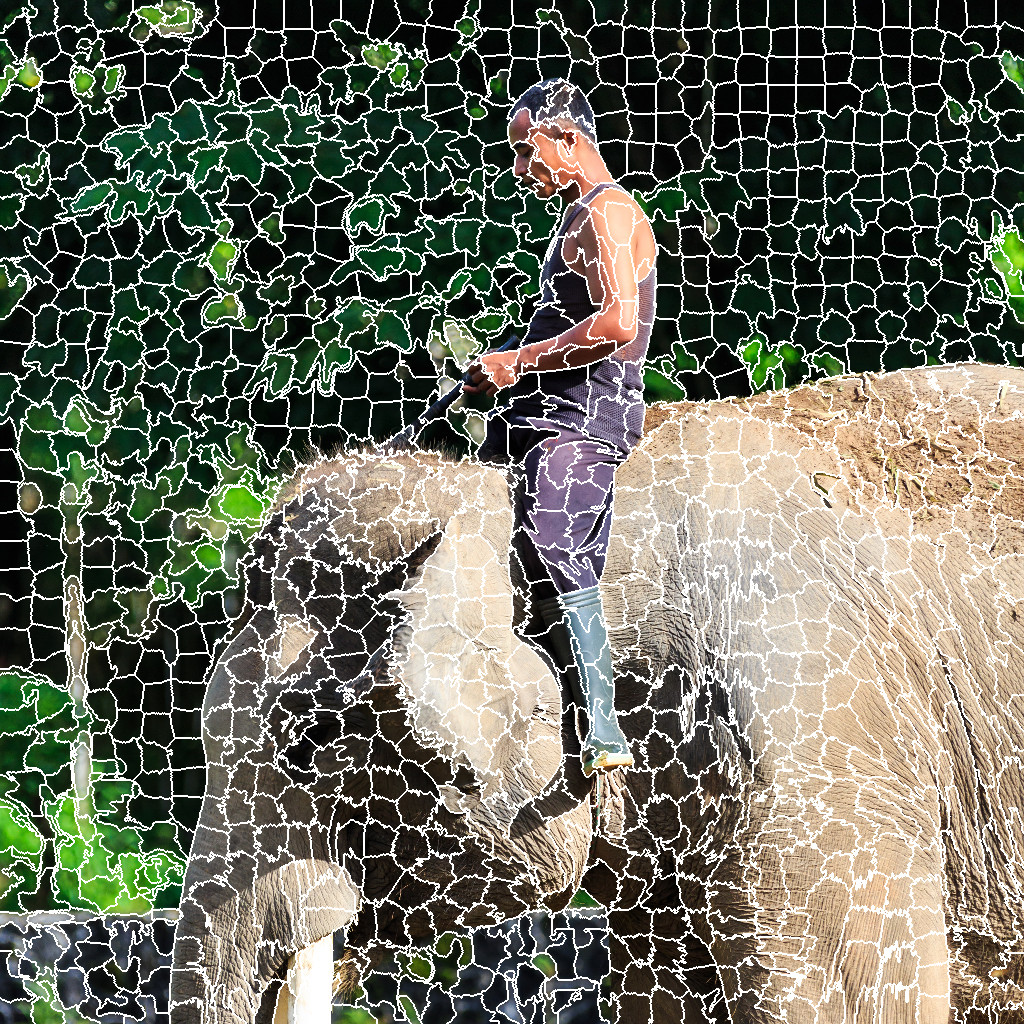
\includegraphics[width=0.65\textwidth]{images/sur-segmentation/exempleSp}
		 \caption{Exemple de sur-segmentation. Les contours des superpixels sont tracés en blanc.}
		 \label{fig:sp_exempleSp}
\end{figure}


\section{Quelques exemples pratiques d'utilisation des superpixels}
L'analyse des méthodes intégrant une étape de sur-segmentation nous semble un préliminaire indispensable pour déduire les propriétés qui doivent être satisfaites par un algorithme de sur-segmentation, afin que celui-ci puisse être utilisé de manière fructueuse. La profusion des travaux reposant sur une étape sur-segmentation interdit toutefois de les décrire de manière exhaustive. Aussi avons-nous choisi trois applications représentatives.

\subsection{Segmentation sémantique}
Publiée en 2008, la méthode de segmentation sémantique de Gould \textit{et al.} \cite{gould2008multi} constitue une étape notable,  tant pour le domaine de la segmentation sémantique que pour celui de la sur-segmentation. Afin d'identifier et de localiser les différents objets composant une photographie, Gould \textit{et al.} proposent une méthode capable, à partir d'un ensemble de données d'apprentissage, de déduire les caractéristiques visuelles d'une catégorie d'objet ainsi que ses relations spatiales avec d'autres types d'objets. Ainsi, la probabilité qu'un ensemble de pixels appartienne à la classe \emph{vache} dépend à la fois de sa couleur, de sa texture et de la présence de pixels voisins attribués à des classes considérées comme probables, telle que \emph{l'herbe}. 

Les motivations évoquées pour justifier l'utilisation de superpixels à la place des pixels rejoignent celles \modif{avancées} par Ren \textit{et al.} \cite{ren2003learning} : la réduction du nombre de primitives manipulées, donc la diminution du temps de calcul global de l'application ainsi que l'utilisation de primitives visuelles contenant une information plus riche. Ainsi, chaque superpixel est décrit à la fois par sa couleur moyenne (\modif{espaces RGB et Lab}), sa texture (\modif{textons}) et sa géométrie. 

Les superpixels étant organisés en graphe, la probabilité pour un superpixel d'appartenir à chacune des classes dépend de ses caractéristiques visuelles propres ainsi que de la probabilité de ses voisins d'appartenir à la même classe ou à une classe fréquemment voisine. Or, contrairement aux pixels qui sont organisés en grille régulière, les superpixels forment un graphe sur lequel peu d'hypothèses simplificatrices peuvent être faites. En particulier\modif{,} la complexité du voisinage d'un superpixel, ou\modif{,} en d'autres termes\modif{,} son nombre de voisins, peut avoir un impact significatif sur le temps d'exécution. 

\subsection{Détection d'obstacle dans un environnement 3D}
Dans leur article \cite{petrovai2014obstacle}, Petrovai \textit{et al.} décrivent un système complet d’assistance à la conduite, capable de générer une représentation 3D de l'environnement dans lequel évolue le véhicule et de s'en servir pour détecter les obstacles présents sur la route, afin d'alerter le conducteur. Pour le rendre indépendant du véhicule, ils utilisent une tablette équipée de deux caméras. Ainsi\modif{,} l'algorithme de détection d'obstacles que Petrovai \textit{et al.} \cite{petrovai2014obstacle} décrivent répond à la nécessité de produire des résultats en temps réel -- permettant au conducteur de réagir promptement -- avec des contraintes matérielles fortes, les tablettes actuelles disposant de capacités de mémoire et de calcul limitées par rapport à celles d'un ordinateur. 

L'environnement 3D est déduit à partir des deux images prises par la tablette, grâce à une méthode de stéréovision : en identifiant pour chaque pixel de l'image de gauche son correspondant dans l'image de droite, la profondeur du point 3D correspondant à ces deux pixels est déduite. Pour des raisons d'efficacité, \modif{seules} quelques correspondances peuvent être identifiées entre les pixels des deux images, par comparaison de leurs caractéristiques. Elles permettent une représentation 3D partielle, qui sera ensuite étendue sur la base de la sur-segmentation en superpixels. Petrovai \textit{et al.} commencent par fusionner ces superpixels  en fonction de leurs similarités en termes de couleur. Puis ils utilisent l'information 3D obtenue à l'étape précédente ainsi qu'une analyse de la géométrie et du niveau de gris moyen des superpixels pour identifier la route et les obstacles, puis pour calculer leur distance par rapport au véhicule. 

Dans le cadre des travaux de Petrovai \textit{et al.}, l'utilisation d'une méthode de sur-segmentation est clairement motivée par la volonté de produire une application finale aussi rapide que possible. Afin d'éviter que des erreurs ne soient commises au moment de la sur-segmentation et propagées, voire amplifiées lors des étapes suivantes, l'algorithme de sur-segmentation est paramétré pour produire des superpixels dont l'aire avoisine les $170$ pixels. 

\subsection{Classification fine d'images}
La classification fine d'images consiste à identifier, à partir d'une photographie, la présence d'objets appartenant à une même catégorie et présentant d'importantes similarités visuelles et sémantiques. Elle trouve de nombreuses applications en biologie,  par exemple pour identifier plusieurs espèces d'oiseaux, ainsi qu'en agronomie,  pour distinguer des plantes malades de celles en bonne santé.  Une part conséquente des travaux de recherche dans ce domaine consiste à proposer des descripteurs capables de \modif{différencier} chaque objet et ce, quel que soit le domaine de classification (champignons, marques de voitures, etc.). Comme les bases de données d'apprentissage peuvent, selon les domaines, contenir un nombre restreint de spécimens, des méthodes reposant sur une étape lourde d'apprentissage à partir d'un ensemble de données de référence \modif{composé} de plusieurs centaines d'images ne sont pas toujours envisageables. 

La méthode de Zhang \textit{et al.} \cite{zhang2016detecting} repose sur l'utilisation de primitives visuelles correspondant à de petits graphes qu'ils nomment \emph{graphlets}. Chaque sommet de ces graphlets correspond à un superpixel, donc un ensemble de pixels. Chaque paire de sommets ayant des pixels \modif{adjacents est} associée par une arête. Les graphlets sont ensuite caractérisés par leurs histogrammes de couleur en neuf dimensions \cite{stricker1995similarity}, leurs histogrammes de gradients orientés \cite{dalal2005histograms} et leurs structures\footnote{Par structure, nous entendons la manière dont \modif{ces} sommets sont connectés entre eux.}.  Pour des raisons de complexité algorithmique, il est souhaitable que les graphlets ne soient composés que d'un petit nombre de sommets. Zhang \textit{et al.} utilisent l'algorithme SLIC \cite{zhang2014probabilistic} proposé par Achanta \textit{et al.} \modif{\cite{achanta2012slic} pour} produire les superpixels. Trois niveaux de sur-segmentation sont produits, le nombre de superpixels, et donc leur aptitude à capter les détails fins, augmentant à chaque niveau.  Ainsi, les graphlets dont les sommets correspondent aux superpixels du premier niveau permettent de décrire les composantes les plus grandes de chaque objet (par exemple le corps d'un oiseau) tandis que ceux comprenant des superpixels du dernier niveau se focalisent sur des éléments plus petits (tels que le bec ou les pattes). Les graphlets comportent un nombre similaire de sommets, quel que soit le niveau de sur-segmentation.

Cette utilisation des superpixels est intéressante pour au moins trois raisons. Tout d'abord, l'un des intérêts  des superpixels réside dans leur faculté à suivre les bordures des objets bien plus finement que des patchs rectangulaires. Avec des séries de photos où le fond peut varier de manière significative, le fait d'utiliser un descripteur qui permette de se focaliser sur l'objet à identifier n'est sans doute pas anecdotique dans les excellents résultats obtenus par la méthode de Zhang \textit{et al.} Ensuite, chaque partie des objets est décrite en utilisant les relations de voisinage des superpixels. Enfin, le fait que trois niveaux de sur-segmentation soient utilisés découle de la difficulté actuelle pour un algorithme de sur-segmentation d'adapter l'aire des superpixels au niveau de détail. 

En effet, pour capter les détails les plus fins, de petits superpixels sont nécessaires. Comme la majorité des méthodes de sur-segmentation produisent des superpixels de taille \modif{quasi uniforme}, l'ensemble de l'image sera découpé en de nombreux superpixels. Au niveau des composantes plus grandes, ce nombre important de superpixels se traduit par des graphlets comprenant de nombreux nœuds, ce qui augmente significativement la complexité des traitements ultérieurs. 

\section{Évaluation d'un algorithme de sur-segmentation}
\subsection{Propriétés à évaluer}

De l'étude des trois applications précédentes, cinq propriétés permettant d'évaluer la qualité d'une sur-segmentation peuvent être énoncées. 
\begin{prop}[validité]
\label{prop1}
une sur-segmentation est considérée comme valide si elle constitue une partition de l'image en sous-ensembles connexes.
\end{prop}

\begin{prop}[adhérence aux contours]
\label{prop2}
un superpixel ne doit pas recouvrir différents objets de l'image.
\end{prop}

\begin{prop}[concision]
\label{prop3}
un algorithme de sur-segmentation doit produire aussi peu de superpixels que possible.
\end{prop}

\begin{prop}[simplicité]
\label{prop4}
le nombre de voisins d'un superpixel doit être aussi petit que possible.  
\end{prop}

\begin{prop}[rapidité]
\label{prop5}
un algorithme de sur-segmentation doit avoir un temps d'exécution aussi faible que possible.
\end{prop}

Pour que ces propriétés soient précises, il reste à définir ce que nous entendons par contour. À la différence d'autres travaux sur la sur-segmentation \cite{machairas2015waterpixels} nous ne pensons pas que ce terme doive se limiter aux contours en termes de couleur ou de  niveau de gris. Au contraire, il nous semble essentiel de prendre en compte la texture,  information dont le bénéfice est connu de longue date \cite{ozden2005image}.

La propriété \ref{prop1} indique que tout pixel doit être associé à un et un seul superpixel et qu'il existe, pour toute paire de pixels $(p_{i},p_{j})$ appartenant à un même superpixel $\mathbf{s}_{k}$, un chemin de pixels \modif{voisins} tous inclus dans $\mathbf{s}_{k}$, reliant $p_{i}$ à $p_{j}$. 

La propriété \ref{prop2} correspond à la définition d'une sur-segmentation : les contours des superpixels incluent les contours des objets dans l'image, mais sont plus nombreux que ces derniers. 

La propriété \ref{prop3} est liée au fait que les superpixels permettent un traitement plus efficace de l'information visuelle contenue dans l'image : moins ils sont nombreux, plus les traitements qui leur sont appliqués sont rapides. 

La propriété \ref{prop4} s'explique par le fait que, contrairement aux pixels, les superpixels ne forment pas un graphe avec une structure régulière en grille, ce qui induit des calculs supplémentaires lorsque le voisinage est pris en compte. Il est donc souhaitable que le nombre moyen de voisins d'un superpixel ne soit pas trop élevé.  

La propriété \ref{prop5} se justifie par le fait que la sur-segmentation d'une image est, dans la majorité des cas, un traitement préalable réalisé dans le but d'abaisser les temps d'exécution d'une méthode. Or le temps nécessaire pour produire les superpixels ne doit pas être supérieur au gain de temps apporté par leur utilisation à la place des pixels. 


\subsection{Évaluations précédentes}
\label{subsec:evalSpStatOfTheArt}

La première évaluation des méthodes de sur-segmentation a été réalisée en 2012 par Achanta \textit{et al.} \cite{achanta2012slic}. Elle compare les méthodes de \modif{Ren \textit{et al.} \cite{ren2003learning}}, Felzenszwalb \textit{et al.} \cite{felzenszwalb2004efficient}, Vedaldi \textit{et al.} \cite{vedaldi2008quick}, \modif{Levinshtein \textit{et al.} \cite{levinshtein2009turbopixels}}, Veksler \textit{et al.} \cite{veksler2010superpixels} et Achanta \textit{et al.} \cite{achanta2012slic}. Les six méthodes sont testées sur les $100$ images de la base de donnée de Berkeley \cite{MartinFTM01}, BSD\footnote{\url{https://www2.eecs.berkeley.edu/Research/Projects/CS/vision/bsds/}}. L'évaluation d'Achanta \textit{et al.} se concentre sur les propriétés \ref{prop2}, \ref{prop3} et \ref{prop5}.  


Afin de quantifier l'adhérence aux contours d'une sur-segmentation (propriété \ref{prop2}), Achanta \textit{et al.} utilisent deux mesures  : le taux d'erreur de sous-segmentation (\modif{$\mathcal{F}_{ES}$}) et le taux de rappel sur les contours (\modif{$\mathcal{F}_{RC}$}).  L'une comme l'autre sont calculées par rapport à une segmentation de référence $R$ à laquelle est comparée la sur-segmentation obtenue. Soit $\mathbb{S}=\lbrace \mathbf{s}_{1},\cdots, \mathbf{s}_{N_{\mathbb{S}}} \rbrace$ l'ensemble des superpixels. Le calcul du taux d'erreur de sous-segmentation repose sur la recherche, pour chaque \modif{région} $r_{i}$ \modif{présente} dans $R$, de l'ensemble des superpixels nécessaires pour le recouvrir et sur le nombre de pixels de cet ensemble  qui débordent de l'objet. Il est défini par : \modif{
\begin{equation}
\label{eq:superpixels:UE}
\mathcal{F}_{ES}(\mathbb{S},R) = \frac{1}{N_{I}} \sum_{r_{i} \in R} \sum_{ \mathbf{s}_{j} \cap r_{i} \neq \emptyset } \min(|\mathbf{s}_{j} \cap r_{i}| ,| \mathbf{s}_{j} - r_{i} |)
\end{equation}}
avec $N_{I}$ le nombre de pixels de l'image.  Le résultat obtenu est compris entre $0$ et $1$, un score de $0$ correspondant à une sur-segmentation sans erreur. 

Le taux de rappel sur les contours permet de vérifier que les contours des objets présents dans $R$ se retrouvent dans $\mathbb{S}$.  Soit $C_{R}$ l'ensemble des points de \modif{contour de la segmentation} de référence et $C_{\mathbb{S}}$ l'ensemble des points de \modif{contour de} la sur-segmentation. Si nous faisons l'hypothèse que\modif{,} pour chaque pixel\modif{,} nous savons sans aucun doute s'il appartient ou non aux contours, nous pouvons évaluer la qualité d'une sur-segmentation en calculant la proportion de points de \modif{contour} dans la \modif{segmentation} de référence qui correspondent à des points de \modif{contour} dans la sur-segmentation  : 
\begin{equation}
\label{eq:superpixels:br}
\mathcal{F}_{RC}(\mathbb{S},R) =   \frac { | C_{\mathbb{S}}  \cap C_{R} | }{ | C_{R} |}\text{.}
\end{equation} 
Concrètement, même pour un être humain, il n'est pas toujours aisé de déterminer au pixel près la position des contours \modif{dans une image}. Achanta \textit{et al.} se donnent une marge de deux pixels. Le score obtenu est compris dans l’intervalle $[0,1]$, un score de $1$ indiquant que tous les contours de $R$ se retrouvent dans $\mathbb{S}$. 

En outre, Achanta \textit{et al.} réalisent une étude de la complexité de chaque méthode ainsi que de ses temps d’exécution (propriété \ref{prop5}). Les scores pour les mesures \modif{$\mathcal{F}_{ES}$ et $\mathcal{F}_{RC}$}, ainsi que les temps d'exécution sont mis en relation avec le nombre de superpixels produits par la méthode, ce qui permet d'identifier les algorithmes capables de satisfaire aux mieux les propriétés \ref{prop2} et \ref{prop5} sous la contrainte de la propriété \ref{prop3}. 

Trois ans plus tard, une seconde évaluation a été menée par Stutz \modif{\textit{et al.} \cite{stutz2015superpixel}}.  Leur première contribution consiste en l'évaluation de 7 méthodes supplémentaires : Liu \textit{et al.} \cite{liu2011entropy},  Zhang \textit{et al.} \cite{zhang2011superpixels}, Conrad \textit{et al.} \cite{conrad2013contour}, Van \textit{et al.} \cite{van2012seeds}, Tang \textit{et al.} \cite{tang2012topology}, Weikersdorfer \textit{et al.} \cite{weikersdorfer2012depth} et Papon \textit{et al.} \cite{papon2013voxel}. Leur seconde contribution réside dans l'utilisation d'une deuxième  \modif{base de données}, celle de l'université de New \modif{York \cite{silberman2012indoor}}, NYU\footnote{\url{http://cs.nyu.edu}}, qui comprend $400$ images. Comme les \modif{tailles} des photographies dans les deux bases de données ne sont pas identiques ($481 \times 321$ pixels pour BSD, $640 \times 480$ pixels pour NYU), Stutz \textit{et al.} proposent de modifier le seuil de tolérance de la mesure $\mathcal{F}_{RC}$ en autorisant tous les pixels à une distance de $\nombre{0,0075} \times diag$, $diag$ \modif{étant la} longueur de la diagonale de l'image.  

Dans l'évaluation d'Achanta \textit{et al.} \cite{achanta2012slic}, les méthodes de Felzenszwalb \textit{et al.} \cite{felzenszwalb2004efficient} et d'Achanta \textit{et al.} \cite{achanta2012slic} obtiennent les meilleurs scores. L'étude de Stutz \modif{\textit{et al.} \cite{stutz2015superpixel}} confirme ce résultat et révèle que les méthodes de Vedaldi \textit{et al.} \cite{vedaldi2008quick}, Conrad \textit{et al.} \cite{conrad2013contour} et  Liu \textit{et al.} \cite{liu2011entropy} obtiennent des scores similaires à ceux de Felzenszwalb \textit{et al.} \cite{felzenszwalb2004efficient} et d'Achanta \textit{et al.} \cite{achanta2012slic}. Sur la base de données BSD, les scores optimaux sont atteints avec des sur-segmentations comprenant un millier de superpixels. Pour les cinq méthodes précédemment citées, le taux d'erreur de sous-segmentation est inférieur ou égal à $\nombre{0,04}$ et le taux de rappel supérieur ou égal à $\nombre{0,99}$. Pour la base de données NYU,  il faut environ $1500$ superpixels à ces mêmes méthodes pour obtenir des scores similaires. Le taux d'erreur de sous-segmentation est inférieur ou égal à $\nombre{0,09}$ et le taux de rappel, là encore, est supérieur ou égal à $\nombre{0,99}$. Pour les deux bases de données, ces performances sont obtenues pour un temps d’exécution d'environ une seconde par image, sur un ordinateur équipé de processeur \emph{Intel Core i7-3770} $\nombre{3,4}$ GHz et d'une RAM de $16$ Go. 

\subsection{Nécessité d'une évaluation complémentaire}
Les résultats obtenus par les deux évaluations précédemment décrites \cite{achanta2012slic, stutz2015superpixel} pourraient nous amener à la conclusion que le problème de la sur-segmentation d'une image est actuellement résolu, cinq méthodes obtenant des scores proches d'un résultat parfait, avec par exemple un taux de rappel de $\nombre{0,99}$ alors que le score maximale atteignable est de $1$. Ces deux évaluations s'avèrent néanmoins critiquables sur deux points : 
\begin{itemize}
\item elles se cantonnent à l'utilisation de petites images de \modif{tailles} similaires (de l'ordre de quelques milliers de pixels) qui ne permettent pas d'apprécier le passage à l'échelle des algorithmes ;
\item  elles se limitent à évaluer l'aptitude des méthodes à produire une sur-segmentation comprenant peu d'erreurs pour un nombre de superpixels donné, sans s'intéresser à leur capacité à s'adapter à la complexité de l'image.
\end{itemize}  

Par \emph{passage à l'échelle} nous entendons le fait qu'un algorithme conserve ses performances quelle que soit la taille de l'image fournie en entrée. En particulier, si les scores évoqués dans la section précédente sont excellents, il est justifié de se demander si les algorithmes évalués conservent la même efficacité avec des images de plusieurs millions de pixels, bien plus proches de la taille des photographies obtenues aujourd'hui avec un appareil photo standard ou un smartphone.

La complexité de l'image désigne ici le nombre d'objets qu'elle contient, ainsi que leur niveau de détail. Nous donnons une illustration de ce concept sur la figure \ref{fig:sp_complexiteImage}, au travers de deux images correspondant à deux situations extrêmes.  Dans le premier cas (figure \ref{fig:sp_complexiteImage}a), nous nous attendons à ce qu'une sur-segmentation en assez peu de superpixels fournisse une compression raisonnable de l'image, où aucune information visuelle importante ne soit perdue. Dans le second cas (figure \ref{fig:sp_complexiteImage}b), la présence de nombreux petits objets, tels que les arbres, ainsi que le niveau de détail sur les bâtiments impose de produire des superpixels plus petits (donc plus nombreux), afin d'éviter que plusieurs superpixels ne chevauchent des objets différents. Cette notion de complexité globale d'une image peut aisément être étendue aux parties d'une même image, à l'instar de l'exemple donné par la figure \ref{fig:sp_complexiteImage}c. Ainsi, si la zone correspondant au ciel peut être sur-segmentée en un nombre restreint de grands superpixels, afin de capter les détails des bâtiments, il est nécessaire de produire de nombreux petits superpixels.
\begin{figure}[htb]
	\centering
	
	 \begin{subfigure}[B]{0.45\textwidth}	
			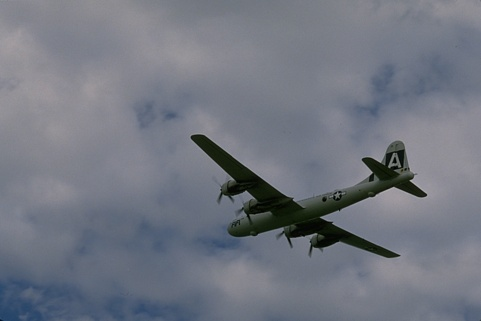
\includegraphics[width=\textwidth]{images/sur-segmentation/im_simple}
		  \caption{Image pouvant être considérée comme simple : un seul objet est visible. Ce dernier contient peu de détails.  Sa couleur comme celle du fond sont relativement uniforme.}
			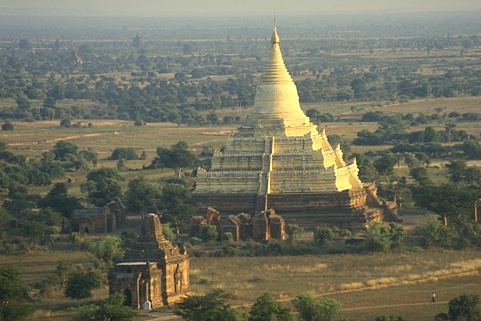
\includegraphics[width=\textwidth]{images/sur-segmentation/im_complexe}
		 \caption{Image pouvant être considérée comme complexe : de nombreux objets sont visibles (les différents bâtiments, les arbres, etc.). En outre, les bâtiments comprennent de nombreux détails. Même pour un être humain, la tâche consistant à tracer le contour de chaque objet visible se révèle fastidieuse. }
	\end{subfigure}		
	~	
	\begin{subfigure}[T]{0.45\textwidth}	
			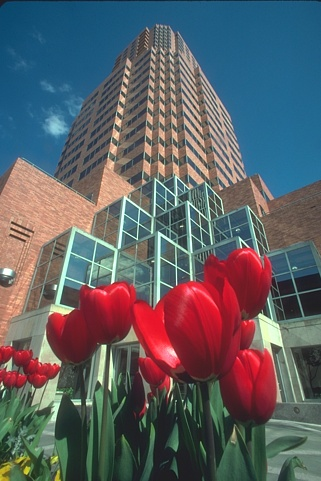
\includegraphics[width=\textwidth]{images/sur-segmentation/im_complexite_variable}
		 \caption{Image contenant des objets de complexité variable : tandis que le ciel correspond à une zone uniforme, les bâtiments contiennent de nombreux détails.  }
	\end{subfigure}
	\caption{Illustration de la notion de complexité à partir de trois photographies issues des données de référence de Berkeley \cite{MartinFTM01}.}
	\label{fig:sp_complexiteImage}
\end{figure}

Dans les trois cas de figure présentés, il est préférable de disposer d'un algorithme de sur-segmentation capable de faire varier automatiquement la taille des superpixels en fonction de la complexité de la zone dans laquelle ils se situent, sans qu'une modification \emph{ad hoc} de ses paramètres ne soit nécessaire. Nous désignons cette capacité d'un algorithme par le terme d'\emph{adaptabilité}. Par la suite, nous verrons que l'analyse de l'adaptabilité d'une méthode de sur-segmentation peut se faire par l'étude de l'évolution conjointe des propriétés \ref{prop2} et \ref{prop3}. 

\section{Proposition d'un nouveau protocole expérimental}
\label{sec:HSID-description-protocole-evaluation}
\subsection{Une nouvelle base de données : HSID}
L'ensemble de données de référence HSID, que   nous avons construit\modif{,} a été \modif{créé} à partir de 100 images issues de la base de données de Wikimedia Commons\footnote{\url{https://commons.wikimedia.org/wiki/Accueil}}. Nous avons sélectionné les photographies pour qu'elles présentent une large variété de difficultés : flou, bruit, ombre, faible contraste, reflet. Pour chacune de ces images, des contours ont été extraits par un être humain. 

Tout d'abord, pour chaque image, les objets qui seront séparés dans la segmentation de référence sont identifiés. Ces derniers sont choisis de manière à correspondre à des objets cohérents. Les objets sélectionnés correspondent aux objets principaux de la photographie ainsi qu'à des objets \modif{au} second plan, mais présentant des difficultés intéressantes.

Ensuite, une segmentation de référence est réalisée, sous forme d’aplats de couleurs, de manière à ce que deux objets voisins aient des couleurs différentes (figure \ref{fig:dataset_creation_step1}). Nous avons utilisé une tablette Intuos Pen ainsi que le logiciel de manipulation d'image Gimp. Enfin, les contours des segmentations sont extraits, un contour correspondant à un pixel ayant au moins un voisin (au sens du 8-voisinage)  de couleur différente (figure \ref{fig:dataset_creation_step2}). Cette dernière étape permet une vérification visuelle de la segmentation de référence créée. Si elle met en évidence des erreurs commises, celles-ci sont corrigées et une nouvelle vérification est effectuée.

\begin{figure}[htb]
	\centering
	 \begin{subfigure}[t]{0.3\textwidth}	
			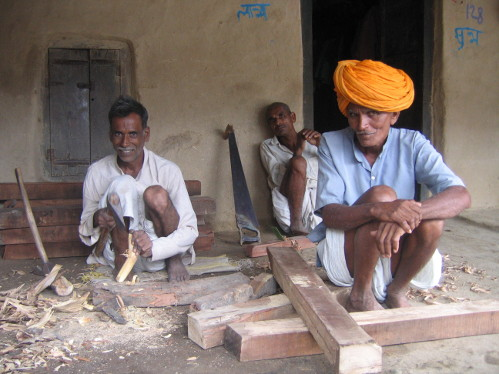
\includegraphics[width=0.95\textwidth]{images/sur-segmentation/HSID/dataset_creation_step0}
		 \caption{Image d'origine}
		 \label{fig:dataset_creation_step0}
	\end{subfigure}		
	~
	 \begin{subfigure}[t]{0.3\textwidth}	
			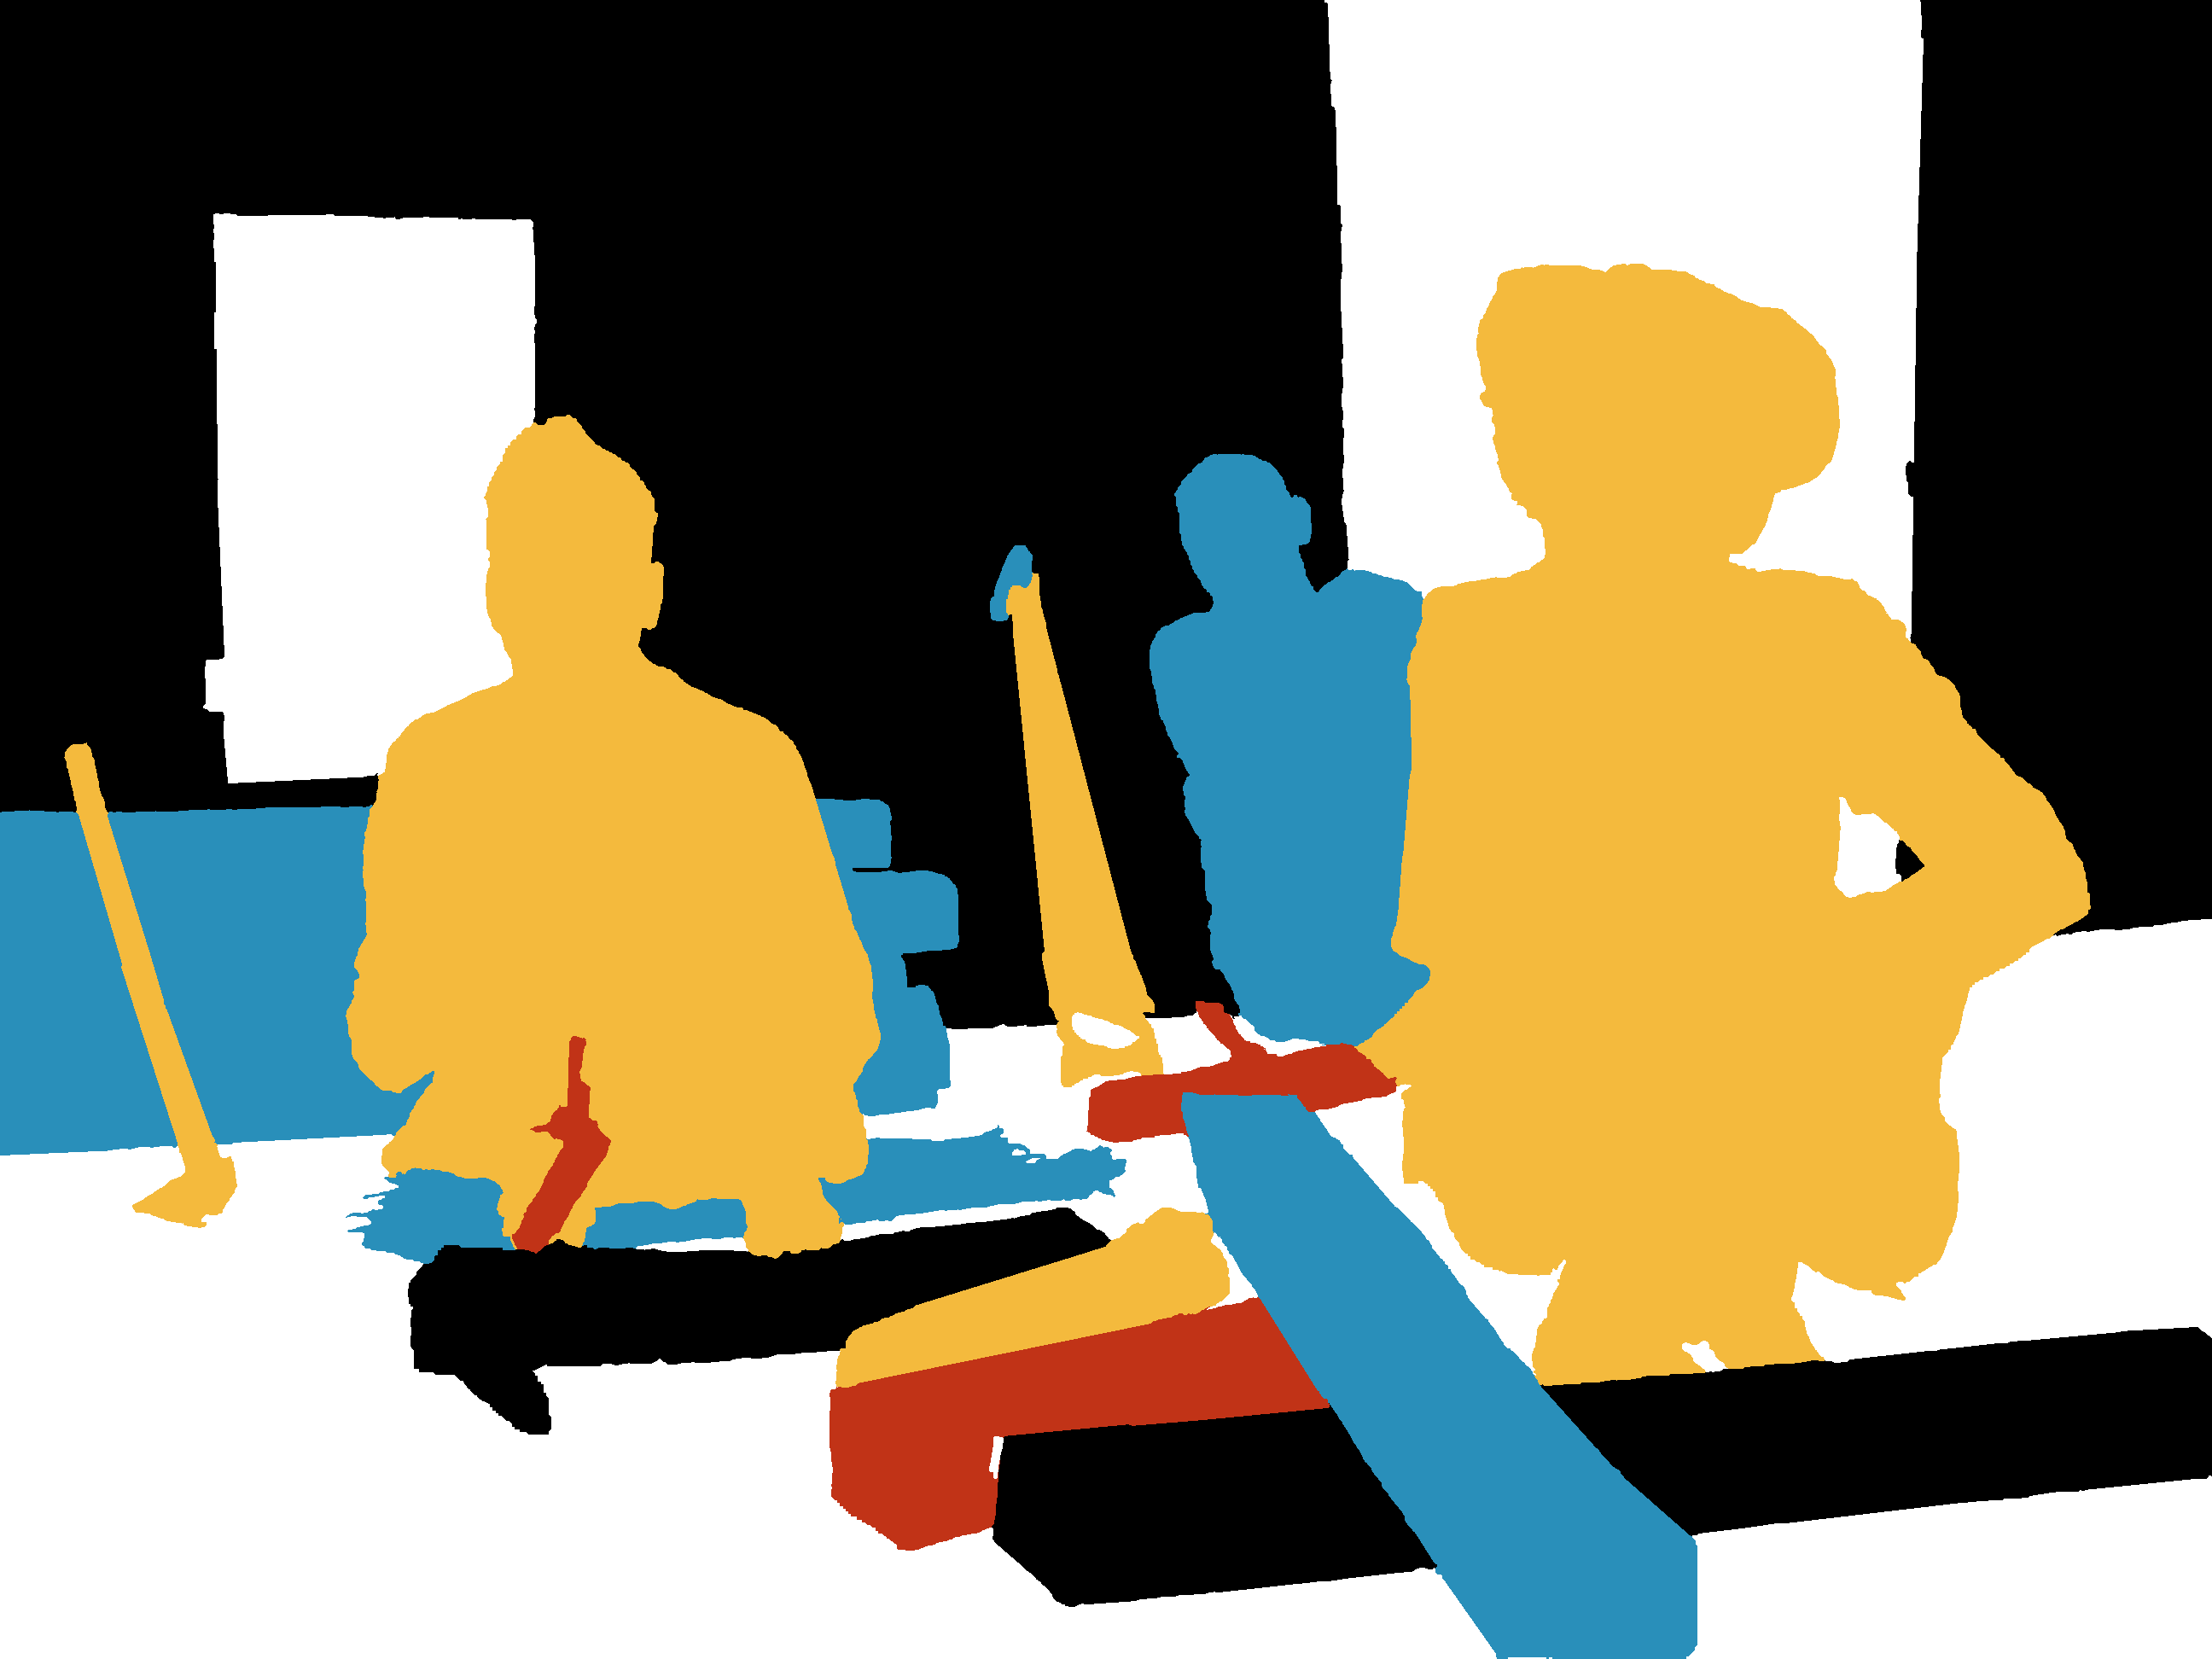
\includegraphics[width=0.95\textwidth]{images/sur-segmentation/HSID/dataset_creation_step1}
		 \caption{Segmentation}
		 \label{fig:dataset_creation_step1}
	\end{subfigure}	
	~
	 \begin{subfigure}[t]{0.3\textwidth}	
			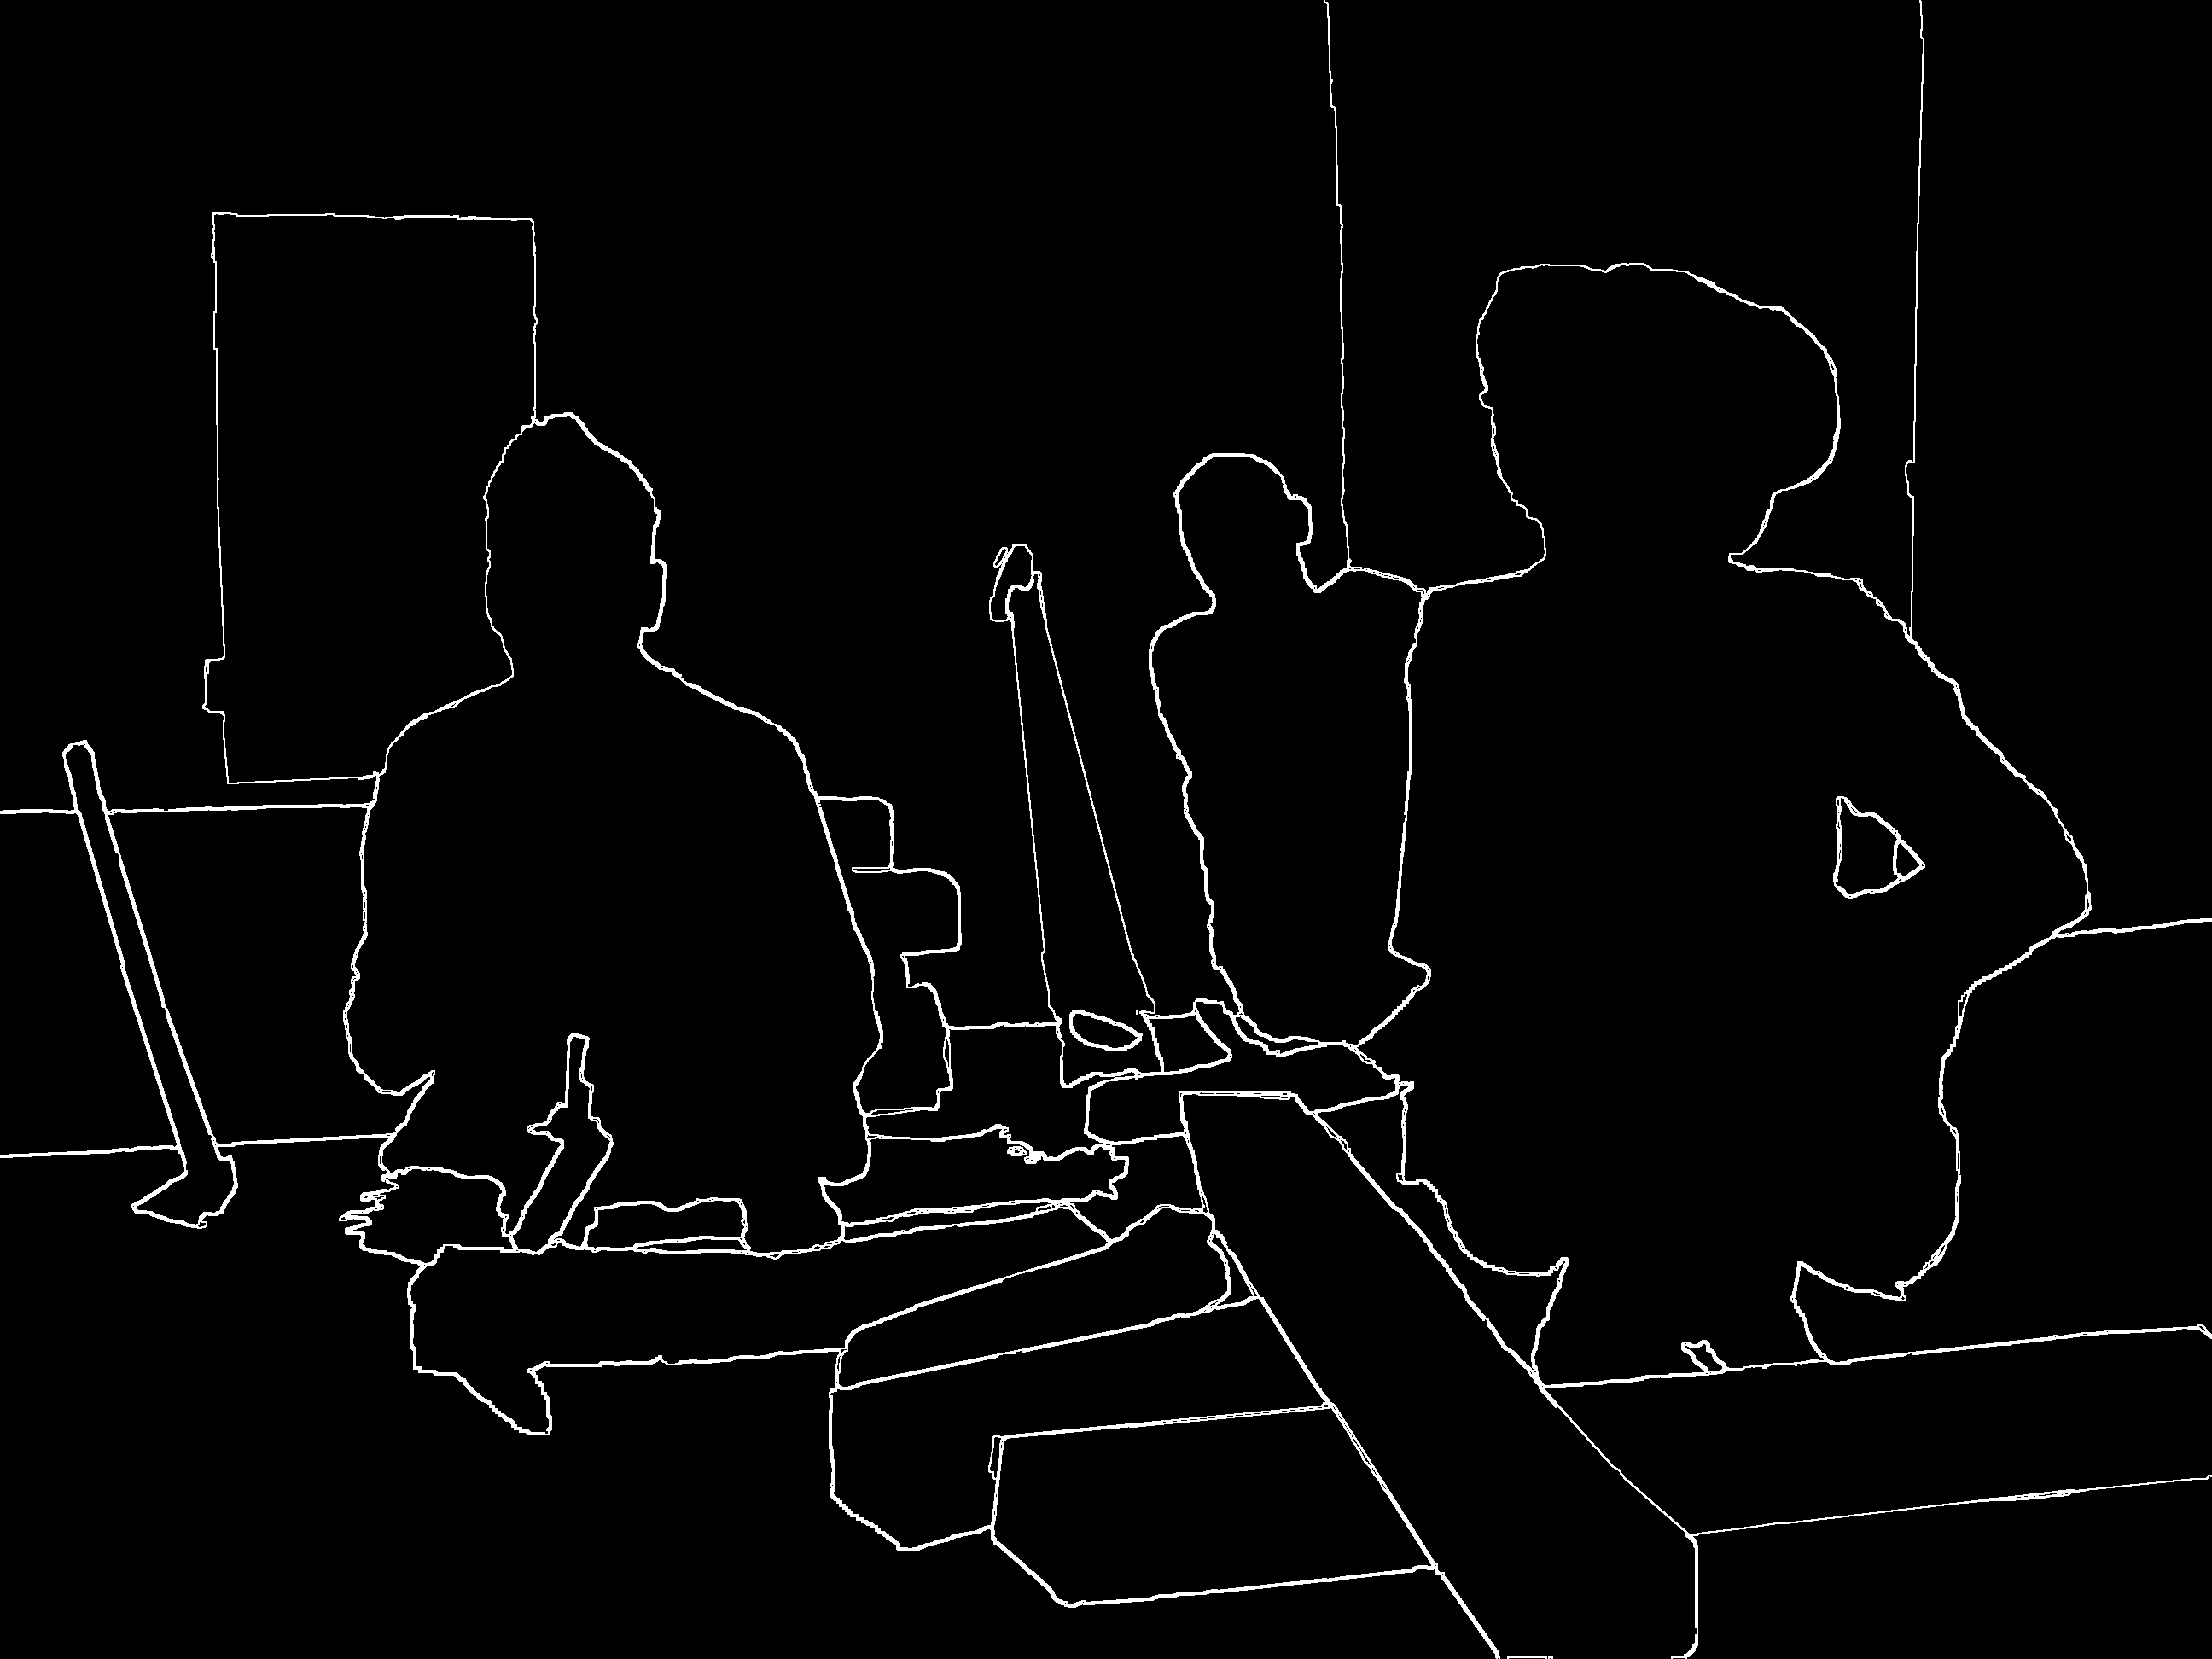
\includegraphics[width=0.95\textwidth]{images/sur-segmentation/HSID/dataset_creation_step2}
		 \caption{Extraction des contours}
		 \label{fig:dataset_creation_step2}
	\end{subfigure}	
	\label{fig:dataset-creation}
	\caption{Procédure suivie pour la création de HSID.}
\end{figure}


\subsection{Mesure de l'adhérence aux contours}

Les mesures d'adhérence aux contours tentent d'évaluer la capacité d'un algorithme de sur-segmentation à produire des superpixels ne chevauchant pas deux objets distincts. Traditionnellement, le taux d'erreur de sous-segmentation $\mathcal{F}_{ES}$ (équation \ref{eq:superpixels:UE}) et la mesure de rappel sur les contours $\mathcal{F}_{RC}$ (équation \ref{eq:superpixels:br}) sont utilisés. Les sections suivantes montrent cependant que HSID soulève des difficultés spécifiques, demandant de repenser ces deux mesures.

\subsubsection{HSID : un cas limite pour l'utilisation du taux d'erreur de sous-segmentation}
La figure \ref{fig:prob-ue} montre deux images de synthèse ($512\times1024$ pixels), correspondant à deux types d'images opposés : la première (figure \ref{fig:img-few-bdr}) contient un seul objet, de grande taille ; la seconde (figure \ref{fig:img-plenty-bdr}) contient de multiples petits objets. Le premier cas correspond à ce que nous obtenons avec une photographie de type portrait, se focalisant sur un seul objet d'intérêt. La seconde situation peut être assimilée à ce que nous obtenons avec une vue panoramique. 
\begin{figure}[htb]
	\centering
	
	 \begin{subfigure}[t]{0.45\textwidth}	
			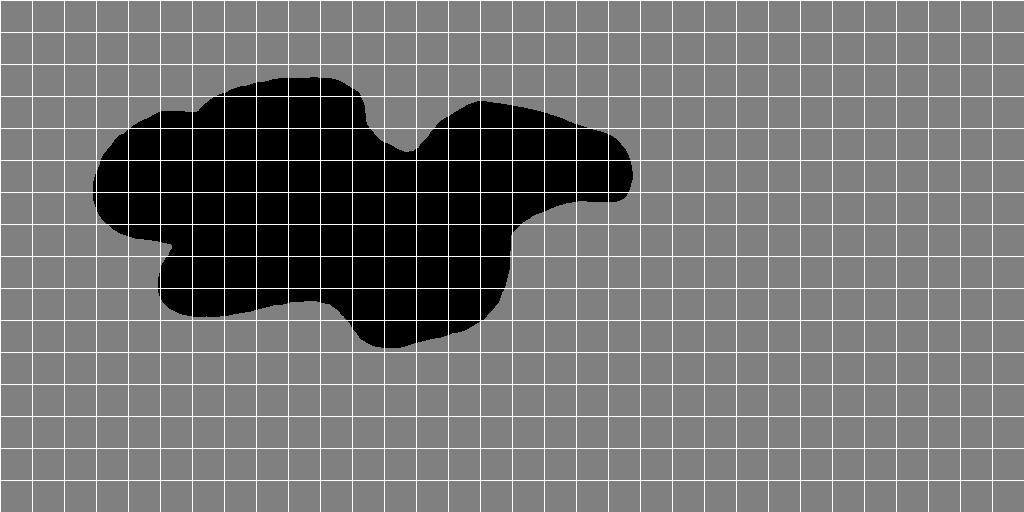
\includegraphics[width=\textwidth]{images/sur-segmentation/UE/01-seg}
		 \caption{Image de type portrait et sur-segmentation sous la forme d'une grille régulière. $\mathcal{F}_{ES}(\mathbb{S},R)=\nombre{0,05}$.}
		 \label{fig:img-few-bdr}
	\end{subfigure}		
	~
	 \begin{subfigure}[t]{0.45\textwidth}	
			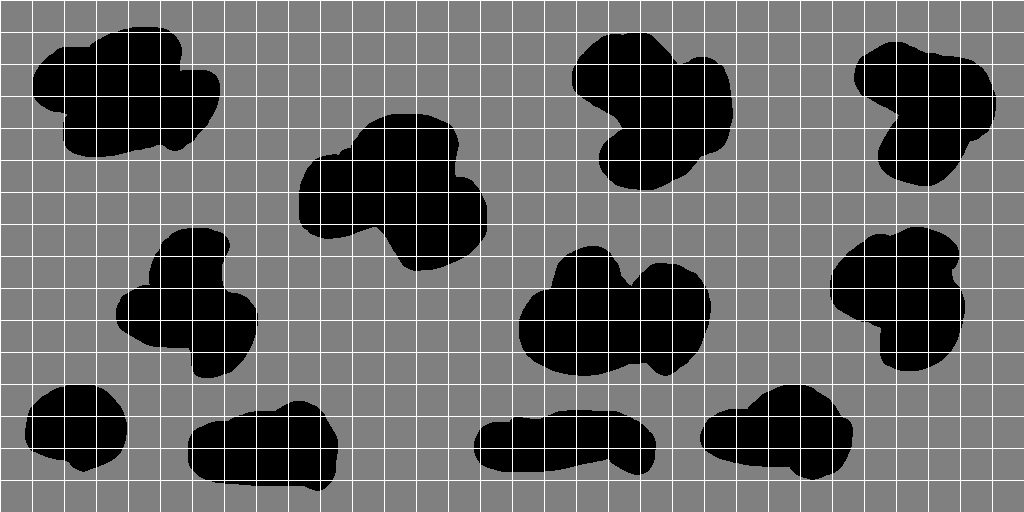
\includegraphics[width=\textwidth]{images/sur-segmentation/UE/10-seg}
		 \caption{Image de type panoramique et sur-segmentation sous la forme d'une grille régulière. $\mathcal{F}_{ES}(\mathbb{S},R)=\nombre{0,1}$.}
		 \label{fig:img-plenty-bdr}
	\end{subfigure}	
	\caption{Images de synthèse mettant en évidence les limites du taux d'erreur de sous-segmentation. Les zones grises correspondent au fond, les zones noires aux objets. Les contours des superpixels sont tracés en blanc. }
	\label{fig:prob-ue}
\end{figure}

Pour ces deux images\modif{,} nous avons produit une sur-segmentation en grille régulière, avec des cases carrées de $32\times32$ pixels. Comme le montre l'affichage des contours de cette sur-segmentation (figure \ref{fig:prob-ue}), dans les deux cas,  la sur-segmentation obtenue comporte de nombreuses erreurs, avec des superpixels dont les contours ne coïncident pas avec ceux des objets visibles. Nous sommes capables de ce diagnostic, car nous focalisons \modif{notre attention} sur les superpixels au niveau des contours des objets. En effet, les superpixels à l'intérieur des différents objets ne contiennent pas d'erreurs et il en serait de même, \modif{quelle que} soit leur forme. Or, ces derniers sont malgré tout pris en compte lors du calcul du taux d'erreur de sous-segmentation $\mathcal{F}_{ES}$, qu'ils contribuent à \modif{diminuer}. Ainsi dans le cas de l'image de la figure \ref{fig:img-few-bdr} où ces superpixels sont plus nombreux, le score $\mathcal{F}_{ES}$ bien meilleur : $\nombre{0,05}$ contre $\nombre{0,1}$ pour l'image de la figure \ref{fig:img-plenty-bdr}.

Les images des données de référence BSD et NYU correspondant essentiellement à des prises de vue panoramiques, le taux moyen d'erreur de sous-segmentation est un indicateur acceptable. Il n'en va pas de même pour HSID, qui comprend les deux situations extrêmes décrites ci-dessus, avec des segmentations de référence allant de deux à une dizaine d'objets. Dans ces conditions, le score moyen, médian, maximum ou minimum obtenu pour la mesure  $\mathcal{F}_{ES}$  ne permet de quantifier correctement l'adhérence aux contours. Nous avons donc choisi de ne pas utiliser la mesure  $\mathcal{F}_{ES}$ .


\subsubsection{Amélioration de la mesure d'adhérence aux contours}

Lors de la réalisation des segmentations de référence, nous avons constaté que, pour un certain nombre des images de HSID, il n'était pas possible de déterminer au pixel près où se situent les contours. C'est par exemple le cas lorsqu'un objet est flou \modif{ou en présence} de fourrure ou de cheveux qui comprennent une part de transparence. 
La grande variété des \modif{tailles} des images \modif{de HSID} rend inutilisable la mesure d'adhérence proposée par Achanta \textit{et al.} \cite{achanta2012slic}, $\mathcal{F}_{RC}$ (équation \ref{eq:superpixels:br})\modif{,} qui utilise un seuil de tolérance fixe, une erreur de deux pixels n'ayant pas du tout la même importance pour une image de $300 \times 400$ pixels que pour une image de $3000 \times 4000$ pixels. Quant à celle proposée par Stutz \textit{et al.} \cite{stutz2015superpixel}, elle s'avère inadaptée pour des images de grande taille, le seuil de tolérance s'élevant alors à une trentaine de pixels, ce qui dépasse largement l'erreur acceptable, y compris dans les pires cas. Ces raisons nous ont conduit à concevoir une nouvelle mesure d'adhérence aux contours, dont la définition s'appuie sur la théorie des sous-ensembles flous. 

Soit $R$  la segmentation de référence pour une image donnée et $\mathbb{S}$  la sur-segmentation obtenue pour cette image. \modif{L'ensemble $R = \lbrace r_{1}, \cdots, r_{N_{R}} \rbrace $} est une partition en $N_{R}$ composantes connexes et \modif{l'ensemble $\mathbb{S}  = \lbrace \mathbf{s}_{1}, \cdots, \mathbf{s}_{N_{\mathbb{S}}} \rbrace$} est une partition en $N_{\mathbb{S}}$ composantes connexes. Nous supposons que $N_{\mathbb{S}} > N_{R}$. 

Un pixel $p_{i}$ est un point de contour dans $\mathbb{S}$, si 
\modif{
\begin{equation*}
\exists p_{j} \in \nei(p_{i})\text{, } ( p_{i} \in \mathbf{s}_{n} \wedge p_{j} \notin \mathbf{s}_{n}) \text{.}
\end{equation*}}

De même, un pixel $p_{i}$ est un point de contour dans $R$, si 
\modif{
\begin{equation*}
\exists p_{j} \in \nei(p_{i})\text{, } ( p_{i} \in r_{n} \wedge p_{j} \notin r_{n}) \text{.}
\end{equation*}}

Soit $C_{R}$  l'ensemble des points de \modif{contour} de $R$ et $C_{\mathbb{S}}$ l'ensemble des points de \modif{contour} de $\mathbb{S}$. La proportion de points de contour de $R$ qui correspondent à des points de contour \modif{de} $\mathbb{S}$ est donnée par \modif{le taux de rappel des contours} $\mathcal{F}_{RC}$ (équation \ref{eq:superpixels:br}).

Comme les points de contour des superpixels qui se situent à l'intérieur d'un objet ne sont pas pris en compte, $\mathcal{F}_{RC}$ est similaire à une mesure d'omission qui serait calculée dans le cadre d'une classification des éléments de $C_{R}$ en deux classes :
\begin{itemize}
\item  \emph{l'élément appartient au contour d'un superpixel} ;
\item  \emph{l'élément n'appartient pas \modif{au} contour \modif{d'un des} superpixels}.
\end{itemize}

Soit \modif{le sous-ensemble} flou $C_{R \cap \mathbb{S}}^{*}$ défini à partir de $C_{R}$, avec la fonction d'appartenance  $f_{R \cap \mathbb{S}}$ qui donne pour un élément de $C_{R}$ son degré d'appartenance à un point de contour dans $C_{\mathbb{S}}$. La fonction $f_{R \cap \mathbb{S}}$  est définie de la manière suivante : 
\modif{\begin{equation}
f_{R \cap \mathbb{S}}(p_{i}) = \exp \left(- \frac{d(p_{i}-p_{i}')^{2}}{2\sigma^{2}} \right)
\end{equation}}
avec  :
\begin{itemize}
\item $d(p_{i}-p_{j})$ la distance entre $p_{i}$  et $p_{j}$  (par exemple la distance euclidienne) ;
\item \modif{$\sigma$ un paramètre pondérant l'influence de la distance entre $p_{i}$  et $p_{j}$, que nous avons fixé à $4$ après quelques tests empiriques} ;
\item \modif{$p_{i}'= \underset{p_{j} \in C_{\mathbb{S}}  } \argmin (d(p_{i}-p_{j}))$}. 
\end{itemize}

La fonction $f_{R \cap S}$ donne une valeur  dans l'intervalle $[0,1]$, la valeur $1$ correspondant au cas où un pixel dans $C_{R}$ coïncide parfaitement avec un pixel dans  $C_{\mathbb{S}}$. Il est \modif{ainsi} possible de définir une mesure floue d'adhérence au contour :
\modif{\begin{equation}
\label{eq:sp:FBR}
\mathcal{F}_{FRC}(\mathbb{S},R)  =  \frac{1}{|C_{R}|} \sum_{p \in C_{R}} f_{R \cap \mathbb{S}}(p)
\end{equation}}
C'est cette mesure que nous proposons d'utiliser pour évaluer l'adhérence aux contours d'une sur-segmentation. 
\section{Algorithmes évalués}

À ce jour, il existe une vingtaine de méthodes de sur-segmentation. Un quart d'entre elles sont initialement des algorithmes de segmentation \modif{\cite{comaniciu2002mean,felzenszwalb2004efficient, ren2003learning,vedaldi2008quick,vincent1991watersheds}} reconvertis grâce à une modification de leurs paramètres. Parmi les méthodes conçues  uniquement pour réaliser une tâche de sur-segmentation, une dizaine \modif{ \cite{achanta2012slic,conrad2013contour,levinshtein2009turbopixels,liu2011entropy,machairas2015waterpixels,papon2013voxel,tang2012topology,van2012seeds,veksler2010superpixels,weikersdorfer2012depth,zhang2011superpixels}} bénéficient d'une bonne notoriété, notamment parce qu'une implémentation ou un exécutable mis à disposition par leurs auteurs facilite leur \modif{réutilisation} au sein d'autres travaux. 

Nous nous sommes concentrés sur les cinq méthodes ayant obtenues les meilleurs scores lors de l'évaluation la plus récente, celle de Stutz \textit{et al.} \cite{stutz2015superpixel} : 
\begin{itemize}
\item la méthode Quick Shift \cite{vedaldi2008quick} (QS), qui consiste en une démarche similaire à celle de l'algorithme mean shift de Comaniciu \textit{et al.} \cite{comaniciu2002mean} ;
\item la méthode de Felzenszwalb \textit{et al.} \cite{felzenszwalb2004efficient} (FZ), qui repose sur un algorithme de coupure de graphe ;
\item la méthode de Liu \textit{et al.} \cite{liu2011entropy} (ERS\modif{, de l'anglais : \og \textit{Entropy Rate Superpixels} \fg}), qui groupe les pixels en ensembles homogènes et de même taille, par maximisation d'une fonction objectif ;
\item la méthode d'Achanta \textit{et al.} \cite{achanta2012slic} (SLIC), dont le traitement principal correspond à l’algorithme des $k$-moyennes et qui est sans doute l'algorithme de sur-segmentation le plus prisé ;
\item la méthode de \modif{Conrad \textit{et al.} \cite{conrad2013contour}} (CRS\modif{, de l'anglais :  \og \textit{Contour Relaxed Superpixels} \fg} ), dont l'originalité consiste à rechercher une sur-segmentation optimale à partir d'une sur-segmentation initiale, en ne modifiant que les pixels en bordure des superpixels. 
\end{itemize}

À ces cinq algorithmes, nous avons ajouté la méthode de Machairas \textit{et al.} \cite{machairas2015waterpixels} (WP\modif{, de l'anglais :  \og \textit{WaterPixels.}\fg}) et celle de Rubio \textit{et al.} \cite{rubio2016bass} (BASS\modif{, de l'anglais :  \og \textit{Boundary-Aware Superpixel Segmentation}\fg}), dont les publications sont concomitantes de celle de l'évaluation de Stutz \textit{et al.} \cite{stutz2015superpixel} et pour lesquelles aucune comparaison complète avec l'état de l'art n'existe. 

\subsection{\modif{Méthode de Vedaldi \textit{et al.} (QS)}}
La méthode QS, proposé par Vedaldi \textit{et al.} \cite{vedaldi2008quick} appartient à la catégorie des algorithmes de segmentation par recherche des modes. Soit $I$ une image. Vedaldi \textit{et al.}  \cite{vedaldi2008quick} décrivent les $N_{I}$ pixels qui la composent par leurs localisations et leurs couleurs. Ils obtiennent alors \modif{$X=\lbrace x_{1}, \cdots, x_{N_{I}} \rbrace$},  un  ensemble de $N_{I}$ vecteurs aléatoires à 5 dimensions. Les modes de la fonction de densité de probabilité associés à ces vecteurs aléatoires correspondent aux instances les plus fréquentes de ces vecteurs (donc aux maxima locaux de cette fonction).

La méthode QS permet de calculer efficacement ces modes et d'associer chaque pixel au mode dont les caractéristiques visuelles sont les plus proches des siennes. Les groupes de pixels ainsi obtenus forment une sur-segmentation de l'image. 

Soit $\phi$, une fonction fenêtre d'observation gaussienne, dont les pondérations sont données par :
\begin{equation}
w_{\phi}(n) = \exp \left( \dfrac{-n^{2}}{2\sigma^{2}} \right)
\end{equation} 
avec :
\begin{itemize}
\item $\dfrac{-(N_{\phi}-1)}{2} < n < \dfrac{(N_{\phi}-1)}{2}$, l'indice de la pondération ;
\item $N_{\phi}$ la taille de la fenêtre ; 
\item $\sigma$ l'écart type de la variable aléatoire considérée.  
\end{itemize}

La méthode QS \cite{vedaldi2008quick} repose sur une estimation de la densité de Parzen :
\modif{\begin{equation}
\mathcal{F}_{P}(x) = \dfrac{1}{N_{I}} \sum_{i=1}^{N_{I}}\phi(d(x - x_{i}))\text{, } x_{i} \in X\text{.}
\end{equation}}
 
À chaque itération de la méthode, chaque point correspondant à un vecteur $x_{i1}$ est déplacé vers $x_{i2}$, son plus proche voisin correspondant à une valeur plus élevée de la fonction de densité de Parzen :\modif{
\begin{equation}
i_{2} = \argmin_{i_{3} \in [1, N_{I}] } d(x_{i1},x_{i3})  \text{, } \mathcal{F}_{P}(x_{i1}) <  \mathcal{F}_{P}(x_{i3}) \text{.} 
\end{equation}}


\subsection{\modif{Méthode} de Felzenszwalb \textit{et al.} (FZ)}

L'algorithme de segmentation proposé par Felzenszwalb \textit{et al.} \cite{felzenszwalb2004efficient} groupe les pixels en régions, de manière à ce que les différences entres les pixels voisins et appartenant à des régions distinctes soient supérieures aux différences entre les pixels appartenant à une même région.

L'image $I$ est modélisée sous la forme d'un graphe \modif{$\mathcal{G}=\ <V,E>$} où $V=\lbrace v_{1},\cdots v_{N_{I}} \rbrace$ est un ensemble de $N_{I}$ sommets correspondant aux pixels de $I$ et $E$ un ensemble d'arêtes pondérées reliant les sommets $v_{i}$ et $v_{j}$ qui correspondent à des pixels voisins. Les régions sont formées en retirant un certain nombre d'arêtes satisfaisant un prédicat, de manière à obtenir une partition de $\mathcal{G}$ en composantes connexes correspondant à des ensembles de pixels homogènes. 


Soit $e_{i,j}$, l'arête reliant les sommets $v_{i}$ et $v_{j}$. La pondération $w_{i,j}$ associée à  $e_{i,j}$ est une mesure de la \modif{dissemblance} entre les pixels $i$ et $j$. Felzenzswalb \textit{et al.} proposent d'utiliser la valeur absolue de la différence entre les niveaux de gris des deux pixels. 


Soit $\mathbf{s}_{i}$ une composante connexe du graphe $\mathcal{G}$ et $E_{i} \subset E$ l'ensemble des arêtes reliant les sommets de  $\mathbf{s}_{i}$. La fonction 
\modif{\begin{equation}
\mathcal{F}_{Int}(\mathbf{s}_{i}) = \max_{e_{j,k} \in E_{i}}(e_{j,k})
\end{equation}}
correspond à une mesure du degré de \modif{dissemblance} entre les pixels composant $\mathbf{s}_{i}$.

Soit $E_{i,j}$ l'ensemble des arêtes reliant un sommet de la composante connexe $\mathbf{s}_{i}$ à un sommet de la composante connexe $\mathbf{s}_{j}$. La fonction 
\modif{\begin{equation}
\mathcal{F}_{Dif}(\mathbf{s}_{i},\mathbf{s}_{j}) = \min_{e_{k,l} \in E_{i,j}}(e_{k,l})
\end{equation}}
correspond à une mesure du degré de \modif{dissemblance} entre les deux composantes connexes $\mathbf{s}_{i}$ et $\mathbf{s}_{j}$. Si $E_{i,j} = \varnothing$, $\mathcal{F}_{Dif}(\mathbf{s}_{i},\mathbf{s}_{j})= \infty$. Le prédicat $\mathcal{F}_{P}$ défini par Felzenszwalb \textit{et al.} \cite{felzenszwalb2004efficient} est une fonction  binaire, qui renvoie \modif{vrai} si les deux composantes connexes doivent rester séparées, \modif{faux} si elles doivent être fusionnées : 
\begin{equation}
\mathcal{F}_{P}(\mathbf{s}_{i},\mathbf{s}_{j}) = \left\{
    \begin{array}{l}
       \text{vrai si } \mathcal{F}_{Dif}(\mathbf{s}_{i},\mathbf{s}_{j}) > \min\Big(\mathcal{F}_{Int}(\mathbf{s}_{i}) + \tau(\mathbf{s}_{i}) ,\mathcal{F}_{Int}(\mathbf{s}_{j}) + \tau(\mathbf{s}_{j})\Big)\text{,}\\
        \text{faux sinon, }
    \end{array}
    \right.
\end{equation}
avec  $\tau(\mathbf{s}_{i}) = \dfrac{\omega_{k}}{|\mathbf{s}_{i}|}$, où $\omega_{k}$ est un paramètre à déterminer lors de l'utilisation de l'algorithme et $|\mathbf{s}_{i}|$ correspond au nombre de sommets composant $\mathbf{s}_{i}$.

\subsection{\modif{Méthode} de Liu \textit{et al.} (ERS)}

L'algorithme ERS \cite{liu2011entropy}, reprend la représentation d'une image $I$ sous forme d'un graphe $\mathcal{G}$, semblable à celui \modif{défini pour la} méthode FZ. De manière similaire, Liu \textit{et al.} \cite{liu2011entropy} cherchent à retirer des arêtes de $E$, afin d'obtenir un ensemble de $N_{S}$ composantes connexes dont chacune correspond à un superpixel. Toutefois, contrairement aux travaux de Felzenszwalb \textit{et al.} \cite{felzenszwalb2004efficient} : 
\begin{itemize}
\item le nombre de composantes connexes est fixé par l'utilisateur et est respecté scrupuleusement par l'algorithme ;
\item les arêtes $e_{i,j} \in E$ sont pondérées par une mesure de similarité au lieu d'une mesure de \modif{dissemblance} ;
\item pour chaque sommet $v_{i}$, est ajoutée une arête $e_{i}$, qui boucle sur ce même sommet : \modif{lorsqu'une arête $e_{i,j}$ est supprimée, sa pondération est ajoutée sur les arêtes $e_{i}$ et $e_{j}$ ($e_{i} \leftarrow e_{i} + e_{i,j}$ et $e_{j} \leftarrow e_{j} + e_{i,j}$ ;}
\item la partition de $\mathcal{G}$ en composantes connexes est obtenue par maximisation d'une fonction objectif \modif{$\mathcal{F}_{ERS}$} : alors que l'algorithme FZ \cite{felzenszwalb2004efficient} repose sur une décision locale (l'arête $e_{i,j}$ \modif{doit-elle} être conservée ou non ?), ERS \cite{liu2011entropy} évalue l'impact global de la suppression de cette même arête.
\end{itemize}

Soit \modif{$\mathcal{G}^{*} =\ <V,E^{*}>$} le graphe résultat correspondant à la sur-segmentation. L'ensemble des arêtes $E^{*}$ correspond au sous-ensemble de $E$ pour lequel la fonction $\mathcal{F}_{ERS}$ atteint son maximum. Liu \textit{et al.} \cite{liu2011entropy} se donnent pour objectif d'obtenir des superpixels :
\begin{itemize}
\item dont les aires, en termes de nombre de pixels, sont similaires ;
\item qui ont une forte homogénéité interne en termes de couleur.  
\end{itemize}
La fonction \modif{de coût} \modif{est :
\begin{equation}
\mathcal{F}_{ERS}(\mathcal{G}') =  \mathcal{F}_{R}(\mathcal{G}') + \mathcal{F}_{E}(\mathcal{G}')
\end{equation}}
où les deux termes \modif{$\mathcal{F}_{R}$ et $\mathcal{F}_{E}$} s'assurent du respect des deux propriétés citées précédemment et $\mathcal{G}' =\ <V,E'> $ est un graphe intermédiaire, avec $E' \in E$.  

Soit $\mathbb{S}=\lbrace \mathbf{s}_{1}, \cdots, \mathbf{s}_{N_{\mathbb{S}}} \rbrace$ une partition de $\mathcal{G}$ en composantes connexes, après avoir supprimé une partie des arêtes de $E$. Nous notons $|\mathbf{s}_{i}|$ la cardinalité d'un ensemble $\mathbf{s}_{i}$. Liu \textit{et al.} \cite{liu2011entropy} définissent\modif{
\begin{equation}
\mathcal{F}_{R}(\mathcal{G}') = -N_{\mathbb{S}} -\sum_{i=1}^{N_{\mathbb{S}}} \dfrac{|\mathbf{s}_{i}|}{|V|}\log\Big( \dfrac{|\mathbf{s}_{i}|}{|V|} \Big) \text{.}
\end{equation}}
Cette fonction favorise non seulement des superpixels ayant la même aire, mais également les partitions des sommets de $V$ en exactement $N_{\mathbb{S}}$ composantes connexes.

Afin de mesurer l’homogénéité interne de chaque superpixel, Liu \textit{et al.} \cite{liu2011entropy} utilisent le taux d'entropie, une mesure qui permet de quantifier le  taux d'incertitude d'un processus aléatoire. Soit $\overline{E'}$ l'ensemble des arêtes supprimées. Les ensembles $E'$ et  $\overline{E'}$ forment une partition de $E$. 

\modif{Soient} $v_{i}$ et $v_{j}$ deux sommets.  Liu \textit{et al.} \cite{liu2011entropy} s'intéressent à la probabilité \modif{$P_{i,j}(\mathcal{G}',E') $} qu'un marcheur partant de $v_{i}$ arrive au sommet $v_{j}$. Cette probabilité est obtenue à partir de la mesure de similarité entre $v_{i}$ et $v_{j}$ :
\modif{\begin{equation}
P_{i,j}(\mathcal{G}',E') = \left\{
    \begin{array}{l l}
       \dfrac{w_{i,j}}{w_{i}} & \text{ si } i \neq j \text{ et } e_{i,j} \in E'\text{,}\\
       0	& \text{ si } i \neq j  \text{ et } e_{i,j} \in \overline{E'}\text{,}\\
       1- \dfrac{1}{w_{i}}  \sum\limits_{\substack{e_{i,k} \in  E'}} w_{i,k} 	& \text{ si } i = j\text{.}
    \end{array}
    \right.
\end{equation}}

\modif{Le graphe $\mathcal{G}'=\ <V,E'>$ peut être modélisé comme une marche aléatoire, sur laquelle il devient possible de calculer le taux d'entropie, mesurant l'homogénéité interne des superpixels} :
\modif{\begin{equation}
\mathcal{F}_{E}(\mathcal{G}',E')  = - \sum\limits_{\substack{v_{i} \in  V}} \left( \dfrac{w_{i}}{w_{V}} \sum\limits_{\substack{v_{j} \in  V}} P_{i,j}(\mathcal{G}',E') \log(P_{i,j}(\mathcal{G}',E'))\right)
\end{equation}}
avec \modif{$w_{V} = \sum\limits_{\substack{v_{i} \in  V}} w_{i}$.}

La recherche du graphe $\mathcal{G}^{*}$ permettant de maximiser $\mathcal{F}_{ERS}$ est réalisée par un algorithme glouton. \modif{En partant d'un ensemble $E'= \varnothing$, les arêtes de l'ensemble $E$ sont progressivement ajoutées à $E'$, en ajoutant à chaque itération l'arête permettant d'aboutir à l'augmentation la plus importante  de $\mathcal{F}_{ERS}$. L'algorithme s'arrête lorsqu'une partition de $V$ en exactement $N_{\mathbb{S}}$ composantes connexes est obtenue. Ces composantes connexes correspondent alors aux superpixels.}

\subsection{\modif{Méthode d'Achanta \textit{et al.} (SLIC)}}
\label{subsec:sp:slic}

La méthode \modif{SLIC} proposée par Achanta \textit{et al.} \cite{achanta2012slic}, correspond à une version modifiée de l'algorithme des $k$-moyennes. Elle est constituée de trois étapes : 
\begin{itemize}
\item l'initialisation, où une première sur-segmentation est donnée ;
\item le regroupement de pixels en ensembles, de manière à ce que chaque pixel soit rattaché à l'ensemble dont les caractéristiques visuelles sont les plus proches des siennes ;
\item le post-traitement s'assurant que les ensembles obtenus à l'étape précédente forment une partition en composantes connexes. 
\end{itemize}

Lors de l'étape d'initialisation, les pixels sont regroupés en superpixels correspondant à un découpage régulier de l'image sous la forme d'une grille. D'autres configurations peuvent également être envisagées, telles que des superpixels hexagonaux. 

La deuxième étape repose sur un processus itératif, répétant une dizaine de fois les actions suivantes :
\begin{enumerate}
\item  la couleur et la position \modif{moyennes} de ces $N_{\mathbb{S}}$ ensembles de pixels correspondant aux superpixels initiaux sont calculées ;
\item chaque pixel, décrit par sa couleur et sa localisation dans l'image, est assigné au superpixel dont il est le plus proche au sens d'une mesure de similarité ;
\item les caractéristiques des superpixels sont mises à jour.
\end{enumerate}

L'une des clés du succès de SLIC réside dans le fait que chaque pixel est comparé uniquement aux ensembles les plus proches, permettant à la méthode de produire une sur-segmentation avec une complexité quasi linéaire vis-à-vis du nombre de pixels dans l'image. 

Soit un superpixel $\mathbf{s}_{i}$ et $p_{j}$ un pixel. Nous notons $l_{i}$, $a_{i}$ et $b_{i}$ la couleur moyenne exprimée dans l'espace CIELab des pixels composant $\mathbf{s}_{i}$ ,  $x_{i}$ et $y_{i}$ les coordonnées du barycentre de $\mathbf{s}_{i}$, $l_{j}$, $a_{j}$ et $b_{j}$  la couleur de $p_{j}$, $x_{j}$ et $y_{j}$ ses coordonnées.  La similarité entre $\mathbf{s}_{i}$ et $p_{j}$ est évaluée par la fonction suivante :
\modif{\begin{equation}
\mathcal{F}_{SLIC}(\mathbf{s}_{i},p_{j}) = \sqrt{\mathcal{F}_{c}(\mathbf{s}_{i},p_{j} )^{2}  + \mathcal{F}_{p}(\mathbf{s}_{i},p_{j})^{2}  \Bigg( \dfrac{\omega_{C} N_{I}}{\sqrt{\omega_{\mathbb{S}}}}\Bigg) ^{2}}
\end{equation}}
avec :
\begin{itemize}
\item \modif{$\mathcal{F}_{c}(\mathbf{s}_{i},p_{j} )  =  \sqrt{(l_{i} - l_{j})^{2} +  (a_{i} - a_{j})^{2} + (b_{i} - b_{j})^{2}}$}, la distance euclidienne entre la couleur moyenne du superpixel et celle du pixel ;
\item  \modif{$\mathcal{F}_{p}(\mathbf{s}_{i},p_{j} )  =  \sqrt{(x_{i} - x_{j})^{2} +  (y_{i} - y_{j})^{2} }$}, la distance euclidienne entre le barycentre du superpixel et la position du pixel ;
\item $N_{I}$ le nombre de pixels de l'\modif{image};
\item \modif{$\omega_{C}$} un paramètre de compacité, pondérant l'influence de la position du pixel par rapport à sa couleur ;
\item $\omega_{N_{\mathbb{S}}}$ un paramètre indiquant le nombre de superpixels souhaités.
\end{itemize}

Soit $\mathbb{S}^{'}$ l'ensemble des superpixels ainsi obtenus. Les pixels étant regroupés aussi en fonction de leur couleur, il n'est pas garanti que  $\mathbb{S}^{'}$ forme une  partition de l'image en composantes connexes. Afin d'assurer le respect de la propriété \ref{prop1} (validité), les composantes connexes de $\mathbb{S}^{'}$  sont extraites. Celles dont le nombre de pixels est en dessous d'une taille minimale sont fusionnées avec une composante connexe voisine, donnant $\mathbb{S}$, la sur-segmentation finale.

\subsection{Méthode de Rubio \textit{et al.} (BASS)}

L'algorithme \modif{BASS de} Rubio \textit{et al.} \cite{rubio2016bass} est une version modifiée de SLIC, capable d'adapter le nombre de superpixels à la complexité locale de l'image : aux endroits contenant des objets de petite taille, de nombreux superpixels sont produits, tandis que les zones uniformes sont sur-segmentées en un nombre restreint de superpixels. Rubio \textit{et al.} introduisent deux changements :
\begin{itemize}
\item le premier, au niveau de l'étape d'initialisation, permet d'adapter le nombre de superpixels  de la sur-segmentation initiale; 
\item le second, au moment de l'évaluation de la similarité est l'ajout d'un terme capable de prendre en compte la présence d'un contour entre un pixel $p_{j}$ et le barycentre de l'ensemble $\mathbf{s}_{i}$.
\end{itemize}

Lors de l'étape d'initialisation, au moment de produire les superpixels initiaux suivant une grille, la méthode de Rubio \textit{et al.} commence par appliquer sur l'image le détecteur de \modif{contour de Doll\'{a}r \textit{et al.}} \cite{dollar2015fast} (évoqué dans la section \ref{subsec:sota:muller}). À partir du résultat de ce détecteur, une image binaire est produite où sont conservés, comme appartenant aux contours, tous les pixels pour lesquels la valeur du détecteur de contours \modif{se situe dans les} $70 \%$ des scores les plus élevés. 

Soit \modif{$\mathcal{F}_{C}$} la fonction qui, pour un ensemble de pixels, donne la portion de pixels appartenant à un contour. En particulier, \modif{$\mathcal{F}_{C}(I)$} correspond à la proportion de pixels appartenant à un contour dans l'image, et \modif{$\mathcal{F}_{C}(\mathbf{s}_{i})$} à celle des pixels appartenant à un contour au sein du superpixel $\mathbf{s}_{i}$. Les deux prédicats suivants permettent d'adapter le nombre de superpixels initiaux à la complexité de l'image :
\begin{itemize}
\item Si \modif{$\mathcal{F}_{C}(\mathbf{s}_{i}) > 3 \mathcal{F}_{C}(I)$}, alors le superpixel $\mathbf{s}_{i}$ appartient à une zone de l'image comprenant de nombreux détails : il est découpé en quatre nouveaux superpixels ;
\item Si  \modif{$\mathcal{F}_{C}(\mathbf{s}_{i}) < \mathcal{F}_{C}(I)$}, alors le superpixel $\mathbf{s}_{i}$ appartient à une zone de l'image relativement homogène et il est supprimé.
\end{itemize}
Afin de terminer l'étape d'initialisation, les composantes connexes correspondant aux  superpixels supprimés sont extraites : elles viennent s'ajouter à l'ensemble des superpixels initiaux, en plus des superpixels conservés et des superpixels nouvellement créés. 

La seconde contribution de Rubio \textit{et al.} consiste à proposer une nouvelle fonction permettant de calculer la similarité entre un superpixel $\mathbf{s}_{i}$ et un pixel $p_{j}$ :
\modif{\begin{equation}
\mathcal{F}_{BASS}(\mathbf{s}_{i},p_{j}) = \sqrt{\mathcal{F}_{c}(\mathbf{s}_{i},p_{j} ) + \omega_{p}\mathcal{F}_{p}(\mathbf{s}_{i},p_{j}) +\omega_{g} \mathcal{F}_{g}(\mathbf{s}_{i},p_{j})}
\end{equation}}
avec :
\begin{itemize}
\item \modif{$\mathcal{F}_{c}$ et $\mathcal{F}_{p}$} les deux fonctions décrites lors de la présentation de l'algorithme SLIC, dans la section précédente ;
\item \modif{$\mathcal{F}_{g}$} une fonction donnant la distance géodésique entre $p_{j}$ et $\mathbf{s}_{i}$ ;
\item $\omega_{p}$ et $\omega_{g}$, deux paramètres permettant de pondérer l'influence de chacun des termes.
\end{itemize}

Soit $p_{i} \in \mathbf{s}_{i}$ et $\zeta_{i,j}=(p_{i},\cdots,p_{j})$ un chemin discret le reliant à $p_{j}$. Soit $\Upsilon_{i,j}$ l'ensemble des chemins reliant $p_{j}$ à un pixel appartenant à $\mathbf{s}_{i}$. Rubio \textit{et al.} définissent :\modif{
\begin{equation}
\mathcal{F}_{g}(\mathbf{s}_{i}, p_{j}) = \min_{ \zeta_{i,j} \in \Upsilon_{i,j}} \sum_{p_{k} \in \zeta_{i,j}} I(p_{k})
\end{equation}}
avec $I(p_{k})$, le niveau de gris du pixel $p_{k}$.

Le déroulement de la deuxième étape de l'algorithme, ainsi que le post-traitement permettant de s'assurer que les superpixels forment une partition en composantes connexes de l'image, restent les mêmes que pour l'algorithme SLIC.

\subsection{\modif{Méthode} de Conrad \textit{et al.} (CRS)}
À l’instar de la méthode Quick Shift, l'algorithme de Conrad \textit{et al.} \cite{conrad2013contour} repose sur la représentation d'une image $I$ par un ensemble de vecteurs \modif{$X=\lbrace x_{1}, \cdots ,x_{N_{I}} \rbrace$}, contenant les caractéristiques visuelles de chaque pixel. Soit \modif{$\mathbb{S}=\lbrace \mathbf{s}_{1,} \cdots, \mathbf{s}_{N_{\mathbb{S}}} \rbrace$} une partition de cette image en $N_{\mathbb{S}}$ superpixels. Les vecteurs qui correspondent aux pixels appartenant à un même superpixel $\mathbf{s}_{i}$ correspondent à un processus stochastique spécifique à $\mathbf{s}_{i}$. Ce processus peut être modélisé sous la forme d'une loi de probabilité de paramètres $\Theta_{i}$. Conrad \textit{et al.} \cite{conrad2013contour}  se donnent une loi de probabilité par composante du vecteur $x_{i}$. L'ensemble des paramètres pour la totalité des superpixels est noté $\Theta$

L'algorithme de Conrad \textit{et al.} \cite{conrad2013contour} repose sur la recherche de la partition $\mathbb{S}^{*}$ et des paramètres $\Theta$ ayant la plus forte probabilité d'avoir généré $X$ :
\begin{equation}
\mathbb{S}^{*} = \argmax_{\mathbb{S}} P(\mathbb{S}, \Theta | X) \text{.}
\end{equation}

Le théorème de Bayes ainsi que le fait que $P(X)$ soit une constante, permettent à Conrad \textit{et al.} d'obtenir :

\begin{equation}
P(\mathbb{S}, \Theta | X) = P(X|\mathbb{S},\Theta) P(\Theta | \mathbb{S}) P(\mathbb{S}) 
\end{equation}
avec :
\begin{itemize}
\item $P(X|\mathbb{S},\Theta)$, la probabilité d'observer l'image $I$, sachant que la partition $\mathbb{S}$ de paramètres $\Theta$ est donnée ;
\item $P(\Theta | \mathbb{S})$, la probabilité que les paramètres $\Theta$ soit corrects, sachant que la partition $\mathbb{S}$ est donnée ;
\item $P(\mathbb{S})$, la probabilité que la partition $\mathbb{S}$ soit correcte. 
\end{itemize}

Les probabilités $P(X|\mathbb{S},\Theta)$ et $P(\Theta | \mathbb{S})$ sont obtenues en modélisant le processus stochastique à l'intérieur de chaque superpixel par une loi de probabilité telle que la loi \modif{g}aussienne ou la \modif{l}oi \modif{l}aplacienne puis en déduisant les paramètres de cette loi à partir de la moyenne et de la variance sur chacune des composantes des vecteurs de l'ensemble $X$. 

Une approximation de la probabilité $P(\mathbb{S})$ est obtenue en pénalisant les pixels adjacents n'appartenant pas au même superpixel : 
\modif{\begin{equation}
P(\mathbb{S}) \propto w_{1} \exp(-n_{4V}w_{4V} § -n_{D}w_{D})
\end{equation}}
avec : 
\begin{itemize}
\item $n_{4V}$ le nombre de paires de pixels voisins, au sens du 4-voisinages, étant attribué à des superpixels différents ;
\item $n_{D}$ le nombre de paires de pixels voisins \modif{diagonaux,} étant attribué à des superpixels différents; 
\item $w_{1}$, \modif{$w_{4V}$, $w_{D}$} des paramètres fixés de manière empirique par Conrad \textit{et al.}
\end{itemize}

Afin \modif{que l'utilisateur puisse choisir} d'obtenir des superpixels plus ou moins réguliers, Conrad \textit{et al.} proposent une version modifiée de la fonction à maximiser :
\modif{\begin{equation}
\label{eq:sp:crs}
\mathcal{F}_{CRS}(\mathbb{S}, X) = P(\mathbb{S}, \Theta | X) + w_{R} \sum_{i=1}^{N_{\mathbb{S}}} \sum_{x_{j} \in \mathbf{s}_{i}} (x_{j}^{p} - x_{i}^{*})^{\top}(x_{j}^{p} - x_{i}^{*})
\end{equation}}
avec $x_{i}^{*}$ le barycentre du superpixel $\mathbf{s}_{i}$, $x_{j}^{p}$ la position du $j\ieme$ pixel et \modif{$w_{R}$} un paramètre fixé de manière empirique.

Comme la recherche de $\mathbb{S}^{*}$ maximisant \modif{la fonction $\mathcal{F}_{CRS}$} n'est pas possible en un temps raisonnable, l'algorithme proposé par Conrad \textit{et al.} \cite{conrad2013contour} recherche une approximation de cette solution optimale en sélectionnant un \modif{sous-ensemble} des pixels sur \modif{les contours} des superpixels  d'une partition et en les attribuant à un superpixel voisin si cela augmente \modif{la valeur de la fonction \modif{$\mathcal{F}_{CRS}$}}. 

Les tests menés par Conrad \textit{et al.} \cite{conrad2013contour} montrent que leur algorithme obtient de \modif{bons} résultats en décrivant chaque pixel par sa couleur exprimée dans l'espace colorimétrique CIELuv.

\subsection{\modif{Méthode} de Machairas \textit{et al.} (WP)}
Les \modif{algorithmes par ligne de partage des eaux (ALPE)} appartiennent à une famille de méthodes de segmentation issues de la morphologie mathématique. Ils reposent sur la modélisation d'une image en niveaux de gris comme un relief topographique puis sur la simulation de l'inondation de ce relief.  Une analogie fréquemment évoquée pour expliquer le principe des ALPE est celui de la ligne continentale de partage des eaux d'Amérique du Nord, qui correspond à une succession de crêtes situées dans les chaînes côtières du Pacifique et les montagnes Rocheuses. Si nous imaginons deux gouttes d'eau tomber de part et d'autre de cette ligne, la première descendra jusqu'à atteindre l'océan \modif{A}tlantique, tandis que la seconde se dirigera vers l'océan \modif{P}acifique : ainsi, cette ligne sépare deux bassins versants, chacun étant associé à un océan. 

De manière similaire, nous pouvons considérer une image en niveau de gris comme un \modif{relief}, les niveaux de gris les plus élevés correspondant aux altitudes les plus hautes. Dans le cas de l'algorithme WP \cite{machairas2015waterpixels}, les différents bassins obtenus donnent une partition de l'image en superpixels, tandis que les lignes de partage des eaux qui les séparent forment les bordures de ces superpixels. La méthode de  Machairas \textit{et al.} \cite{machairas2015waterpixels} \modif{repose} sur une modélisation de l'inondation par immersion : les niveaux de gris les plus faibles forment des sources depuis \modif{lesquelles} l'eau s'écoule pour remplir petit à petit les bassins versants. Les lignes de partage des eaux correspondent aux \modif{endroits} où les eaux provenant de deux bassins différents se rencontrent.

Afin de simuler ce processus d'immersion, les pixels de l'image sont triés par ordre \modif{décroissant de leurs niveaux de gris}. Soit $\min(I)$, le plus petit niveau de gris de l'image $I$. Soit  \modif{$CC^{\min(I)}$}, l'ensemble des composantes connexes formées par les pixels ayant le niveau de gris  $\min(I)$ et \modif{$CC^{\min(I)+1}$}, l'ensemble des composantes connexes formées par les pixels ayant un niveau de gris inférieur ou \modif{égal} à $\min(I)+1$. Soit \modif{$cc_{i}^{\min(I)+1} \in CC^{\min(I)+1}$} une composante connexe à traiter :
\begin{itemize}
\item si \modif{$\forall \ cc_{j}^{\min(I)} \in CC^{\min(I)} \text{ : } cc_{j}^{\min(I)} \cap cc_{i}^{\min(I)+1} = \varnothing$ }, alors \modif{$cc_{i}^{\min(I)+1}$} correspond à un nouveau \modif{minimum} de $I$ et forme un nouveau bassin versant (un exemple de cette configuration est donné \modif{sur la figure} \ref{fig:sp:wp}a) ;
\item si \modif{$\exists cc_{i}^{\min(I)}\text{, } \forall \ cc_{k}^{\min(I)} \in CC^{\min(I)} \text{ avec } k \neq i \text{ : } cc_{j}^{\min(I)} \cap cc_{i}^{\min(I)+1} \neq \varnothing \  \wedge cc_{j}^{\min(I)} \cap cc_{k}^{\min(I)+1} = \varnothing $}, alors \modif{$cc_{j}^{\min(I)}$ et $cc_{i}^{\min(I)+1}$} appartiennent au même bassin versant  (un exemple de cette configuration est donné \modif{sur la figure} \ref{fig:sp:wp}b) ;
\item \modif{si $ \exists \ cc_{j}^{\min(I)} \neq cc_{k}^{\min(I)} \text{, } cc_{j}^{\min(I)} \cap cc_{i}^{\min(I)+1} \neq \varnothing \wedge cc_{k}^{\min(I)} \cap cc_{i}^{\min(I)+1} \neq \varnothing$}, alors $CC^{\min(I)+1}$ contient plusieurs bassins versants, un par \modif{composante} connexe de $CC^{\min(I)}$ incluse dans $CC^{min(I)+1}$  (un exemple de cette configuration est donné \modif{sur la figure} \ref{fig:sp:wp}c).
\end{itemize}
Lorsque le troisième cas de figure se produit, les éléments de \modif{$CC^{\min(I)+1}$} doivent être répartis entre les différent\modif{s} bassins versants. Machairas \textit{et al.} utilisent la notion de zone d'influence géodésique pour réaliser cette répartition. 

\begin{figure}[htb]
	\centering
	 \begin{subfigure}[t]{0.3\textwidth}	
			
\includegraphics[width=\textwidth]{images/sur-segmentation/immerssionSim1}
		 	\caption{Découverte d'un nouveau bassin versant.}
	\end{subfigure}
	~
	 \begin{subfigure}[t]{0.3\textwidth}	
			
\includegraphics[width=\textwidth]{images/sur-segmentation/immerssionSim2}
		 \caption{Agrandissement d'un bassin versant existant. }
	\end{subfigure}
	~
	 \begin{subfigure}[t]{0.3\textwidth}	
			
\includegraphics[width=\textwidth]{images/sur-segmentation/immerssionSim3}
		 \caption{Deux bassins versants au sein d'une même composante connexe.}
	\end{subfigure}
	\caption{Les trois cas de \modif{figure} possibles lors de la recherche de bassins versants par simulation d’\modif{inondation.}}
	\label{fig:sp:wp}
\end{figure}

Soit $A$ un ensemble et $x$ et $y$ deux éléments de $A$.  La distance géodésique entre $x$ et $y$ correspond à la \modif{longueur du plus petit chemin} reliant $x$ à $y$ et n'étant constitué que d'éléments inclus dans $A$. \modif{Soit $B$ et $C$, deux composantes connexes dont les tous les éléments sont inclus dans $A$ (c'est-à-dire que $B \subset A$ et $C \subset A$). Supposons que les éléments de $B$  et de $C$ sont parfaitement distincts. Soit $D$ le complémentaire de $B \cup C$, contenant tous les éléments de $A$ n'appartenant ni à $B$ ni à $C$. Soit $d_{i} \in D$. Soit $b_{i}$ (respectivement $c_{i}$), l'élément de $B$ le plus proche de $d_{i}$ au sens de la distance géodésique (respectivement l'élément de $C$ le plus proche de $d_{i}$ au sens de la distance géodésique). Si $b_{i}$ est plus proche de $d_{i}$ que $c_{i}$, alors $d_{i}$ appartient à la zone d'influence de $B$. Si $b_{i}$ et $c_{i}$ sont à égale distance de $d_{i}$ alors cet élément appartient au squelette des zones d'influences de $B$ et de $C$. 
} 


Ce procédé d'immersion est répété du niveau de gris le plus faible jusqu'au niveau de gris le plus élevé, afin d'obtenir une partition de l'image en superpixels. 

\section{Résultats de l'évaluation}

Les sections suivantes présentent les résultats obtenus par chacun des algorithmes évalués. Pour chaque méthode, nous avons réalisé 8 tests, en faisant varier les paramètres de manière à ce que le nombre moyen de superpixels de l'image soit respectivement proche de 500 (test 1), 700 (test 2), 900 (test 3), 1100 (test 4), 1300 (test 5), 1500 (test 6), 1700 (test 7) et 1900 (test 8) superpixels. Chaque test est effectué avec l'ensemble des images de HSID. 

 Dans les paragraphes suivants nous noterons :
\begin{itemize}
\item $N_{\mathbb{S}}$ le nombre de superpixels ;
\item $N_{V}$ : le nombre de voisins d'un \modif{superpixel} ;
\item $T$ : le temps d'exécution de la méthode ;
\item \modif{$\mathcal{F}_{FRC}$ : le score obtenu avec la mesure floue d'adhérence aux contours (équation \ref{eq:sp:FBR})}.
\end{itemize}

L'ensemble des algorithmes évalués respectant par construction la propriété \ref{prop1} (validité), nous ne nous attarderons pas sur cette dernière. La mesure $\mathcal{F}_{FRC}$ permet d'apprécier la capacité d'un algorithme à satisfaire la propriété \ref{prop2} (adhérence aux contours). Un score moyen proche de $1$ et un écart type faible, indiquent que la méthode évaluée sur-segmente correctement l'ensemble des images de HSID. 

La mise en relation de cette mesure avec le nombre de superpixels $N_{\mathbb{S}}$ conduit à une analyse du respect de la propriété \ref{prop3} (concision), en identifiant les méthodes capables d'obtenir une bonne adhérence aux contours tout en conservant un nombre peu élevé de superpixels. 

La mesure $N_{V}$ permet d'évaluer le respect de la propriété \ref{prop4} (simplicité) : il est souhaitable que le score moyen et l'écart type obtenus pour cette mesure soient aussi bas que possible.

La propriété \ref{prop5} (rapidité) est, quant à elle, évaluée à l'aide de la mesure $T$ du temps d’exécution.

Tous les algorithmes évalués ont obtenu d'excellents scores avec les mesures et les données de référence des deux évaluations précédentes \cite{achanta2012slic,stutz2015superpixel}. Le constat d'une performance moindre sur HSID, avec les mesures précédemment présentées, peut donc venir :
\begin{itemize}
\item d'une difficulté à traiter des images de grande taille, avec notamment un écart type important pour les mesures $T$ et $\mathcal{F}_{FRC}$ ;
\item d'une difficulté à traiter avec les mêmes paramètres des images de tailles \modif{différentes}, ce qu'indiqueraient des écarts types importants pour les mesures $N_{V}$, $T$ et $\mathcal{F}_{FRC}$.
\end{itemize}

Dans les deux cas, nous considérons que la méthode ne passe pas à l'échelle, puisque l'introduction d'images de taille importante se révèle problématique. 

Reste la question de l'adaptabilité d'une méthode, c'est-à-dire de sa capacité à sur-segmenter correctement des images de différentes complexités ou des images dont certaines zones sont plus complexes que d'autres. Une manière d'identifier les algorithmes possédant cette propriété consiste à s'intéresser à l'écart type de la mesure $N_{\mathbb{S}}$. Nous nous attendons à ce que ce dernier soit élevé, un faible écart type indiquant que la méthode est restée très proche du nombre moyen de superpixels recherché, sans s'adapter aux données.

L'ensemble des sur-segmentations produites par chacun des algorithmes peut être consulté en ligne\footnote{\url{http://image.ensfea.fr/hsid/}}.

\subsection{Quelques résultats généraux}

Sur l'ensemble des tests, tous les algorithmes produisent des sur-segmentations avec en moyenne $6$ voisins par superpixel, avec un écart type inférieur à $\nombre{0,2}$. En ce qui concerne la propriété de simplicité, les méthodes évaluées réalisent donc une performance équivalente.

Les figures \ref{fig:sp:fbr_nbSp} et \ref{fig:sp:time_nbSp} montrent, pour chaque algorithme, l’évolution de l'adhérence aux contours en fonction du nombre de superpixels.  Le score $\mathcal{F}_{FRC}$ donné correspond à la moyenne obtenue pour l'ensemble de HSID. Les méthodes ERS, FZ et SLIC réalisent une performance significativement meilleure que celles des algorithmes QS, CRS, BASS et WP. Dans les sections suivantes, nous aurons l'occasion d'analyser plus en détail ce que ces résultats impliquent. 


\begin{figure}[htb]
	\centering	
			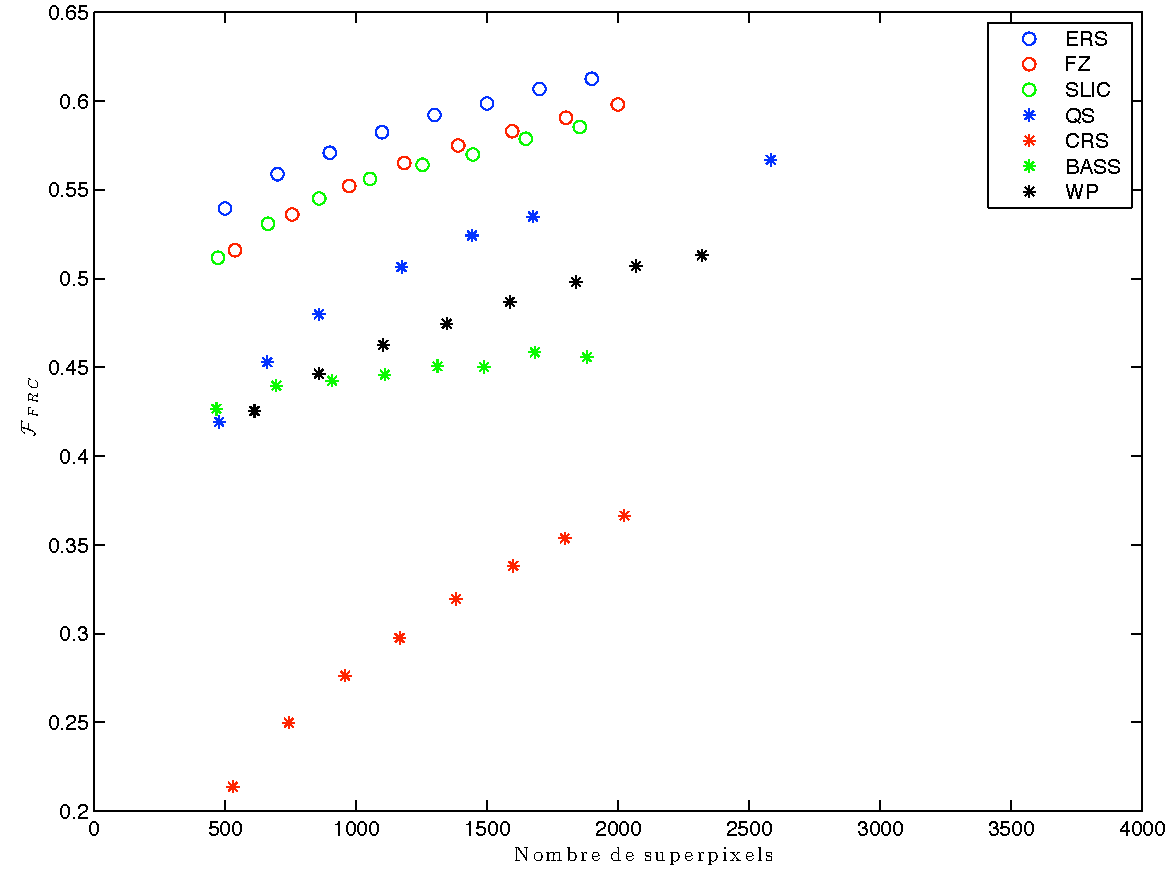
\includegraphics[width=\textwidth]{images/sur-segmentation/fbr_NbSp}
		 	\caption{Évolution de l'adhérence aux contours ($\mathcal{F}_{FRC}$) en fonction du nombre de superpixels.}
		 	\label{fig:sp:fbr_nbSp}
\end{figure}

La figure \ref{fig:sp:time_nbSp} donne les temps \modif{d'exécution} moyens de chaque algorithme en fonction du nombre de superpixels.  Les deux extrêmes sont\modif{,} d'une part\modif{,} l'algorithme QS dont le temps d'exécution moyen dépasse la minute et\modif{, d'autre part,} SLIC dont la durée moyenne est de seulement $3$ secondes. Par rapport aux évaluations précédemment menées \cite{achanta2012slic, stutz2015superpixel}, nos tests font apparaître de manière nette les différences entre \modif{les algorithmes}. 

À part QS pour lequel une variation importante est visible, le nombre de superpixels produits n'influe que peu le temps d'exécution moyen. En effet, la complexité algorithmique des méthodes étudiées dépend essentiellement du nombre de pixels. 

\begin{figure}[htb]
	\centering	
			\includegraphics[width=\textwidth]{images/sur-segmentation/time_NbSp}
		 	\caption{\modif{Évolution du temps d'exécution} en fonction du nombre de superpixels.}
		 	\label{fig:sp:time_nbSp}
\end{figure}

\subsection{\modif{Méthode de Vedaldi \textit{et al.} }}

Pour évaluer la méthode QS  \cite{vedaldi2008quick}, nous avons utilisé l'implémentation de la bibliothèque VLFeat\footnote{\url{http://www.vlfeat.org/overview/quickshift.html}}. Trois paramètres doivent être spécifiés :
\begin{itemize}
\item $\omega_{c}$, qui permet de pondérer l'importance de la couleur du pixel par rapport à sa position dans l'image ;
\item $\omega_{\phi}$, qui correspond à la taille de la fenêtre d'observation gaussienne ;
\item $\omega_{d}$, qui est la distance maximale entre deux pixels $p_{i}$ et $p_{j}$ pour que $p_{j}$ soit considéré comme appartenant \modif{à l'ensemble des} plus proches voisins de $p_{i}$.
\end{itemize}

Durant les 8 tests, nous avons utilisé $\omega_{c}=\nombre{0,75}$ et $\omega_{\phi}=3$, qui correspondent aux valeurs recommandées par Stutz \textit{et al.} \cite{stutz2015superpixel} lors de leur évaluation. Le tableau \ref{tab:sp:paramQS} récapitule les valeurs utilisées pour le paramètre $\omega_{d}$.

\begin{table}[htb]
 \caption{Valeurs du paramètre $\omega_{d}$ utilisées pour évaluer la méthode QS\modif{.}}
\centering
\begin{tabular}{| l| l| l| l| l| l| l| l|  l|}
\hline
\cellcolor{gris}{Test} & 1 & 2 & 3 & 4 & 5 & 6&7 &8\\
\hline
$\cellcolor{gris}{\omega_{d}}$ & 47 & 50 &35 &30 &27 &25&20 &10\\
\hline
\end{tabular}
\label{tab:sp:paramQS}
\end{table}


L'analyse de la figure \ref{fig:sp:fbr_nbSp} montre que l'algorithme QS obtient la quatrième position en termes de respect de l'adhérence aux contours par rapport au nombre de superpixels. Le score $\mathcal{F}_{FRC}$ moyen obtenu pour chacun des tests reste significativement inférieur à celui des algorithmes ERS, FZ et SLIC.  Le tableau \ref{tab:sp:minmaxSpQS} montre que l'écart entre le nombre minimum de superpixels  et le nombre maximum de superpixels  pour chaque test est conséquent. 

\begin{table}[htb]
 \caption{Bornes de l'intervalle de variation du nombre de superpixels produits par l'algorithme QS.}
\centering
\begin{tabular}{| l| l| l| l| l| l| l| l|  l|}
\hline
\cellcolor{gris}{Test} & 1 & 2 & 3 & 4 & 5 & 6&7 &8\\
\hline
\cellcolor{gris}{min} & $12$  & $16$ &$24$ &$29$ &$38$ &$42$&$65$ &$80$\\
\hline
\cellcolor{gris}{max} &  $2045$  & $2768$ &$3596$ &$4750$ &$5803$ &$6763$&$10222$ &$13969$\\
\hline
\end{tabular}
\label{tab:sp:minmaxSpQS}
\end{table}

La figure \ref{fig:sp:qs:nbsp_pixels} permet de voir qu'il existe une corrélation entre le nombre de pixels et le nombre de superpixels produits. Si nous étudions l'ensemble des sur-segmentations produites par Quick Shift, nous constatons  que les images de grande taille produisent des sur-segmentations avec davantage de superpixels que les images de petite taille. Nous n'avons par ailleurs pas su trouver de relation simple entre $\omega_{d}$ et $N_{I}$, le nombre de pixels de l'image, qui permette d'obtenir un nombre de superpixels pertinent. Cette dépendance entre l'un des paramètres de Quick Shift et \modif{la taille} de la photographie traitée se révèle problématique lorsque les \modif{tailles} des images à sur-segmenter \modif{n'est pas connue} à l'avance, notamment lorsque ces dernières proviennent de sources diverses. C'est en particulier le cas pour le domaine d'application qui nous intéresse : celui de la segmentation interactive.

Le faible score d'adhérence aux contours s'explique par le problème évoqué précédemment :  pour les petites images, le nombre de superpixels n'est pas assez important pour permettre une sur-segmentation précise, \modif{ ce qui se répercute sur la moyenne du score $\mathcal{F}_{FRC}$.} Par ailleurs, les images contenant des objets dont les contours ne sont pas nets, notamment parce qu'ils représentent des animaux à fourrure ou les cheveux d'une personne, posent également de grosses difficultés à Quick Shift. 

\begin{figure}[htb]
	\centering	
			\includegraphics[width=\textwidth]{images/sur-segmentation/QS/spEvolution}
		 	\caption{Algorithme QS : évolution du nombre de superpixels par rapport au nombre total de pixels dans l'image.}
		 	\label{fig:sp:qs:nbsp_pixels}
\end{figure}

La figure \ref{fig:sp:exqs1} illustre ce phénomène. Elle montre les superpixels obtenus pour deux images. Dans les deux cas, le paramètre $\omega_{d}$ vaut $47$. Pour la figure \ref{fig:sp:exqs1}a, qui correspond à une photographie de $732 \times 509$ pixels, nous obtenons $57$ superpixels. Au contraire, la photographie de la figure \modif{\ref{fig:sp:exqs1}b}, qui contient $3648 \times 2736$ pixels, est sur-segmentée en $1204$ superpixels. Enfin, le temps d'exécution moyen, même s'il décroît à mesure que le nombre de superpixels augmente, se classe parmi les plus élevés, certaines images nécessitant plusieurs minutes pour être sur-segmentées.

\modif{Ces résultats nous conduisent} à conclure que, malgré ses bonnes performances dans les études précédentes, la méthode Quick Shift ne passe pas à l'échelle et échoue à sur-segmenter convenablement HSID.

 
\begin{figure}[htb]
	\centering
	 \begin{subfigure}[t]{0.6\textwidth}	
			\includegraphics[width=\textwidth]{images/sur-segmentation/QS/Ex1-img-100}
		 	\caption{Superpixels obtenus pour l'image img-100 de HSID. Cette image comporte $732 \times 509$ pixels.}
	\end{subfigure}
 \\
	 \begin{subfigure}[t]{0.6\textwidth}	
			\includegraphics[width=\textwidth]{images/sur-segmentation/QS/Ex2-img-041}
		 	\caption{Superpixels obtenus pour l'image img-041 de HSID. Cette image comporte $3648 \times 2736$ pixels.}
	\end{subfigure}
	\caption{Algorithme Quick Shift : exemples de sur-segmentations obtenues lors du test 1, pour des images de tailles différentes. }
	\label{fig:sp:exqs1}
\end{figure}

 \subsection{Algorithme de Felzenszwalb \textit{et al.}}
 
Afin d'évaluer l'algorithme de Felzenszwalb \textit{et al.} \cite{felzenszwalb2004efficient}, nous avons utilisé l'implémentation mise à disposition par les auteurs. Elle nécessite de fixer trois paramètres : 
 \begin{itemize}
 \item  $\omega_{k}$ qui pondère l'influence des différences internes à une composante connexe, par rapport aux différences entre deux composantes connexes ;
 \item $\omega_{\sigma}$, le paramètre du filtre gaussien qui, lors d'un prétraitement, permet de réduire le bruit au sein des images ;
 \item $\omega_{min}$, la taille minimale des superpixels. 
 \end{itemize}
 
 Lors de l'ensemble de nos tests, nous avons utilisé $\omega_{k} = 24$ et $\omega_{\sigma}=\nombre{0,5}$. Ces deux paramètres découlent de tests effectués sur deux autres ensembles d'images : celles mises à disposition par McGuinness \textit{et al.} \cite{mcguinness2010comparative} et celles de Santner \textit{et al.} \cite{santner2010interactive}, les paramètres trouvés par Stutz \textit{et al.} ne se révélant pas pertinents pour HSID. Pour le paramètre $\omega_{min}$, nous avons utilisé les valeurs données dans le tableau \ref{tab:sp:paramFZ}. 

\begin{table}[htb]
 \caption{Valeurs du paramètre $\omega_{min}$ utilisées pour l'algorithme de Felzenszwalb \textit{et al}. La variable $N_{I}$ correspond au nombre de pixels de l'image. }
\centering
\begin{tabular}{| l| l| l| l| l| l| l| l|  l|}
\hline
\cellcolor{gris}{Test} & 1 & 2 & 3 & 4 & 5 & 6&7 &8\\
\hline
$\cellcolor{gris}{\omega_{min}}$ & $ N_{I}/2500$ &  $ N_{I}/3500$  & $ N_{I}/4500$  & $ N_{I}/5500$  & $ N_{I}/6500$  & $N_{I}/7500$ &  $ N_{I}/7500$ & $ N_{I}/8500$ \\
\hline
\end{tabular}
\label{tab:sp:paramFZ}
\end{table}

Les résultats obtenus par l'algorithme FZ \modif{montrent} qu'il permet de garantir une bonne adhérence aux contours. Pour l'ensemble des tests, nous constatons un écart type élevé pour la mesure $N_{\mathbb{S}}$, égal à environ un cinquième de la valeur de la moyenne. Mis en relation avec les bons scores d'adhérence aux contours, ce résultat révèle que l'algorithme de Felzenszwalb \textit{et al.} bénéficie d'une bonne adaptabilité, ce que confirme l'étude des sur-segmentations produites et ce qu'illustrent les deux exemples de la figure \ref{fig:sp:exfz1}.
 
 L'un des reproches fréquemment adressés à la méthode de Felzenszwalb \textit{et al.} concerne l'aspect des superpixels qu'elle produit, avec des bordures souvent très sinueuses, donnant un aspect moins visuellement plaisant que des algorithmes tels que SLIC ou celui de Liu \textit{et al.}. Les superpixels de la figure \ref{fig:sp:exfz1} sont effectivement assez irréguliers. De plus, la topologie des deux sur-segmentations présente des aspects surprenants tels qu'un superpixel inclus à l'intérieur d'un autre superpixel de grande taille. La  moyenne et l'écart type de la mesure $N_{V}$ révèlent toutefois qu'en termes de nombre de superpixels voisins, l'algorithme de Felzenszwalb produit des résultats similaires à ceux des autres algorithmes évalués, avec un score de $6$, ce qui reste inférieur au nombre de voisins \modif{d'un} pixel si nous considérons le 8-voisinage.

Le  temps d'exécution moyen de l'algorithme gravite autour d'une dizaine de secondes et tend à diminuer légèrement lorsque le nombre de superpixels augmente. 

L'ensemble de ces résultats nous conduit à conclure que l'algorithme de Felzenszwalb \textit{et al.} passe correctement à l'échelle, en réussissant à sur-segmenter les images de HSID de manière à conserver une bonne adhérence aux contours, sans que le nombre de superpixels n'explose. 
 
 \begin{figure}[htb]
	\centering
	 \begin{subfigure}[t]{0.55\textwidth}	
			\includegraphics[height=0.4\textheight]{images/sur-segmentation/FZ/EX1-img-086}
		 	\caption{Superpixels obtenus pour l'image img-086 de HSID.}
	\end{subfigure}
	~ 
	 \begin{subfigure}[t]{0.4\textwidth}	
			\includegraphics[height=0.4\textheight]{images/sur-segmentation/FZ/EX2-img-028}
		 	\caption{Superpixels obtenus pour l'image img-028 de HSID.}
	\end{subfigure}
	\caption{Algorithme de Felzenszwalb \textit{et al.} : exemples de sur-segmentations obtenues lors du test 8. }
	\label{fig:sp:exfz1}
\end{figure}
 
 \subsection{Algorithme de Liu \textit{et al.}}
 Pour évaluer l'algorithme de Liu \textit{et al.} \cite{liu2011entropy}, nous avons utilisé l'implémentation fournie par les auteurs ainsi que les paramètres recommandés par Stutz \textit{et al.} \cite{stutz2015superpixel}. Les paramètres à spécifier sont les suivants :
 \begin{itemize}
 \item $\omega_{\sigma}$, qui correspond à l'écart type d'une fonction gaussienne utilisée pour calculer la mesure de similarité entre deux pixels à partir de la valeur absolue de la différence entre les niveaux de gris des pixels ;
 \item $\omega_{\lambda}$, qui permet de pondérer l'influence entre les termes $\mathcal{F}_{R}$ et $\mathcal{F}_{E}$ de la \modif{fonction de coût} ;
 \item $\omega_{N_{\mathbb{S}}}$, le nombre de superpixels souhaité. 
 \end{itemize}
 

 Durant tous les tests, nous avons considéré des pixels voisins au sens du 8-voisinage, $\omega_{\sigma}=\nombre{0,21}$ et $\omega_{\lambda}=\nombre{0,5}$. Pour le paramètre $\omega_{N_{\mathbb{S}}}$, nous avons utilisé les valeurs présentées dans le tableau \ref{tab:sp:paramERS}.
 \begin{table}[htb]
 \caption{Valeurs du paramètre $\omega_{N_{\mathbb{S}}}$ utilisées pour évaluer l'algorithme de Liu \textit{et al.}}
\centering
\begin{tabular}{| l| l| l| l| l| l| l| l|  l|}
\hline
\cellcolor{gris}{Test} & 1 & 2 & 3 & 4 & 5 & 6&7 &8\\
\hline
$\cellcolor{gris}{\omega_{N_{\mathbb{S}}}}$ & 500 & 700 & 900 &1100 &1300 &1500&1700 &1900\\
\hline
\end{tabular}
\label{tab:sp:paramERS}
\end{table}

 
De toutes les méthodes évaluées, celle de Liu \textit{et al.} obtient la meilleure adhérence aux contours avec un minimum de superpixels. Cette très bonne performance doit cependant être nuancée par  des temps d'exécution importants (plus d'une minute pour certaines images) et l'absence complète d'adaptabilité, le nombre de superpixels étant un paramètre fixé par l'utilisateur de la méthode. Le premier de ces inconvénient limite l'utilisation de la méthode à des applications où les temps de calcul ne sont pas trop critiques. Ce n'est malheureusement pas le cas du domaine applicatif qui nous intéresse, celui de la segmentation interactive. Quant à l'absence d'adaptabilité, elle se traduit par deux désavantages : d'une part, certaines images relativement simples sont sur-segmentées en davantage de superpixels que nécessaire. D'autre part, pour les images les plus complexes, même avec $1900$ superpixels, certains détails sont perdus.
 
  \begin{figure}[htb]
	\centering
	 \begin{subfigure}[t]{0.45\textwidth}	
			\includegraphics[width=\textwidth]{images/sur-segmentation/ERS/EX1-img-042}
		 	\caption{Superpixels obtenus pour l'image img-042 de HSID.}
	\end{subfigure}
 ~
	 \begin{subfigure}[t]{0.45\textwidth}	
			\includegraphics[width=\textwidth]{images/sur-segmentation/ERS/EX2-img-058}
		 	\caption{Superpixels obtenus pour l'image img-058 de HSID.}
	\end{subfigure}
	\caption{Algorithme de Liu \textit{et al.} : exemples de sur-segmentations obtenues lors du test 6. }
	\label{fig:sp:exers1}
\end{figure}
 

 Les deux exemples présentés sur la figure \ref{fig:sp:exers1} soulignent ce paradoxe : si les sur-segmentations produites suivent parfaitement les contours des objets, malgré le fait que les photographies présentent de nombreuses difficultés (objets voisins de couleurs similaires, bruit, ombre, etc.), elles comprennent de nombreux petits superpixels qui pourraient être fusionnés. 
 
 \subsection{\modif{Méthode  d'Achanta \textit{et al.}}}
\label{subsec:sp:res-slic}
 
 Afin d'évaluer l'algorithme SLIC \cite{achanta2012slic}, nous avons utilisé l'implémentation mise à disposition par Achanta \textit{et al.} Cette dernière requiert de spécifier : 
 \begin{itemize}
 \item \modif{$\omega_{C}$}, le paramètre de compacité pondérant l'influence de la localisation d'un pixel par rapport à sa couleur ; , le nombre approximatif de superpixels souhaité, qui permet de produire la sur-segment
 \item $\omega_{N_{\mathbb{S}}}$, le nombre approximatif de superpixels souhaité, qui permet de produire la sur-segmentation de départ, sous forme de grille.
 \end{itemize}
 
Suivant les recommandations d'Achanta \textit{et al.} \cite{achanta2012slic} et celles de Stutz \textit{et al.} \cite{stutz2015superpixel}, nous avons utilisé \modif{$\omega_{C} = 10$} pour l'ensemble de nos tests. Les valeurs du paramètre  $\omega_{N_{\mathbb{S}}}$ sont données dans le tableau \ref{tab:sp:paramSLIC}.

 \begin{table}[htb]
 \caption{Valeurs du paramètre $\omega_{N_{\mathbb{S}}}$ utilisées pour évaluer l'algorithme SLIC.}
\centering
\begin{tabular}{| l| l| l| l| l| l| l| l|  l|}
\hline
\cellcolor{gris}{Test} & 1 & 2 & 3 & 4 & 5 & 6&7 &8\\
\hline
$\cellcolor{gris}{\omega_{N_{\mathbb{S}}}}$ & 500 & 700 & 900 &1100 &1300 &1500&1700 &1900\\
\hline
\end{tabular}
\label{tab:sp:paramSLIC}
\end{table}


 SLIC nécessite davantage de superpixels que les algorithmes de Felzenszwalb \textit{et al.} \cite{felzenszwalb2004efficient} et de Liu \textit{et al.} \cite{liu2011entropy} pour obtenir une adhérence aux contours semblable, avec un score $\mathcal{F}_{FRC}$ égal à $\nombre{0,59}$ atteint avec \modif{quasiment} $1900$ superpixels, tandis que les deux méthodes précédemment citées réalisent la même performance avec respectivement $1600$ et $1300$ superpixels. En termes d'adaptabilité, l'algorithme de Felzenszwalb se révèle également légèrement meilleur que SLIC \modif{: adapter le nombre de superpixels au niveau de détail de l'image reste à la charge de l'utilisateur.} Le principal atout de SLIC reste cependant ses temps d'exécution, largement \modif{inférieurs} à ceux des autres méthodes, avec un temps moyen de $3$ secondes.

 
  \begin{figure}[htb]
	\centering
	 \begin{subfigure}[t]{0.45\textwidth}	
			\includegraphics[width=\textwidth]{images/sur-segmentation/SLIC/EX1-img-046}
		 	\caption{Superpixels obtenus pour l'image img-046 de HSID.}
	\end{subfigure}
 ~
	 \begin{subfigure}[t]{0.45\textwidth}	
			\includegraphics[width=\textwidth]{images/sur-segmentation/SLIC/EX2-img-052}
		 	\caption{Superpixels obtenus pour l'image img-052 de HSID.}
	\end{subfigure}
	\caption{Algorithme SLIC: exemples de sur-segmentations \modif{obtenues lors du test 8}.}
	\label{fig:sp:exslic1}
\end{figure}


  \subsection{Algorithme de Rubio \textit{et al.}}
Afin de tester l'algorithme de Rubio \textit{et al.} \cite{rubio2016bass}, nous avons utilisé l'implémentation mise à disposition par ses auteurs. Le seul paramètre de cette méthode est $\omega_{N_{\mathbb{S}}}$, le nombre initial de superpixels, pour lequel nous avons utilisé les valeurs du tableau \ref{tab:sp:BASSParam}.

\begin{table}[htb]
\caption{Valeurs du paramètre $\omega_{N_{\mathbb{S}}}$ utilisées lors des tests effectués avec la méthode de Rubio \textit{et al.}}
\centering
\begin{tabular}{|l|l|l|l|l|l|l|l|l|}
\hline
\cellcolor{gris}{\modif{Test} }& 1 & 2 & 3 &4 & 5&6 &7 &8 \\
\hline
$\cellcolor{gris}{\omega_{N_{\mathbb{S}}}}$&700&1100&1500&1900&2300&2700&3100&3500 \\
\hline
\end{tabular}
\label{tab:sp:BASSParam}
\end{table}

L'analyse des résultats de l'algorithme de Rubio \textit{et al.}, permet de mettre en exergue l'importance de la mise à disposition de HSID. Dans l'article \cite{rubio2016bass} où ils décrivent leur algorithme, Rubio \textit{et al.} le comparent à quelques méthodes de l'état de l'art, dont SLIC, sur sept \modif{ensembles de données de référence différents} \modif{\cite{kolesnikov2014closed,liu2011learning,MartinFTM01,yamaguchi2012parsing,yan2014hierarchical}}, totalisant plusieurs milliers d'images comprenant des difficultés très variées mais dont les \modif{tailles} sont toujours \modif{proches} : quelques centaines de pixels en largeur comme en hauteur, pour un nombre total de pixels $N_{I} \backsimeq 15000$. Une autre propriété commune à l'ensemble des photographies est qu'elles contiennent en majorité des objets bénéficiant d'un bon contraste avec le fond. Les résultats obtenus par Rubio \textit{et al.} montrent que leur méthode obtient de meilleurs résultats que SLIC, avec un nombre \modif{inférieur de superpixels.} 

Nos tests avec HSID ne permettent pas d'aboutir à la même conclusion :  le score d'adhérence aux contours de la méthode de Rubio \textit{et al.} est largement en dessous de celui de SLIC. Les deux exemples donnés sur la figure \ref{fig:sp:exbass1} montrent que les mécanismes qui garantissent à l'algorithme de Rubio \textit{et al.} une bonne adaptabilité sont responsables des erreurs importantes commises, là où la présence des contours des objets est difficilement perceptible.

Par ailleurs, les modifications introduites par Rubio \textit{et al.} afin d'obtenir une méthode avec une meilleure adaptabilité se paient par une augmentation considérable des temps d’exécution, avec une moyenne d'environ $40$ secondes, soit plus de dix fois le temps d'exécution moyen de SLIC. Notons que les algorithmes de Felzenszwalb \textit{et al.} \cite{felzenszwalb2004efficient} et de Liu \textit{et al.} \cite{liu2011entropy} (avec lesquels Rubio \textit{et al.} ne comparent pas leur méthode), obtiennent eux aussi une bien meilleure adhérence aux contours, avec des temps d'exécution inférieurs.
 
 
   \begin{figure}[htb]
	\centering
	 \begin{subfigure}[t]{0.45\textwidth}	
			\includegraphics[width=\textwidth]{images/sur-segmentation/BASS/EX1-img-012}
		 	\caption{Superpixels obtenus pour l'image img-012 de HSID.}
	\end{subfigure}
 ~
	 \begin{subfigure}[t]{0.45\textwidth}	
			\includegraphics[width=\textwidth]{images/sur-segmentation/BASS/EX2-img-040}
		 	\caption{Superpixels obtenus pour l'image img-040 de HSID.}
	\end{subfigure}
	\caption{Algorithme de Rubio \textit{et al.}: exemples de sur-segmentations \modif{obtenues lors du test~1}.}
	\label{fig:sp:exbass1}
 \end{figure}

 \subsection{Algorithme de Conrad \textit{et al.}}
 
 Afin de tester l'algorithme de Conrad \textit{et al.} \cite{conrad2013contour}\modif{,} nous avons utilisé l'implémentation que les auteurs ont mise à disposition. Les paramètres de cette implémentation sont les suivants :
 \begin{itemize}
 \item $\omega_{R}$, le paramètre permettant de pondérer l'influence du terme de régularisation de la fonction à maximiser ;
 \item $\omega_{4V}$, le paramètre permettant de pondérer la pénalité prise en compte lorsque l'un des quatre voisins d'un pixel n'appartient pas au même superpixel ;
 \item $\omega_{D}$, le paramètre permettant de pondérer la pénalité prise en compte lorsque l'un des voisins diagonaux d'un pixel n'appartient pas au même superpixel ;
 \item $\omega_{Iter}$, le nombre d'itérations de l'algorithme ;
 \item $\omega_{N_{\mathbb{S}}}$, le nombre initial de superpixels.
 \end{itemize}
 Pour l'ensemble de nos tests, nous avons utilisé $\omega_{R}=\nombre{0,045}$, $\omega_{4V}=\nombre{0,3}$, $\omega_{D}=\nombre{0,21}$ et $\omega_{Iter}=3$, valeurs recommandées par Stutz \textit{et al.} \cite{stutz2015superpixel}. Pour le paramètre $\omega_{N_{\mathbb{S}}}$ nous avons utilisé les valeurs données dans le tableau \ref{tab:sp:CRSParam}.
  \begin{table}[htb]
\caption{Valeurs du paramètre $\omega_{N_{\mathbb{S}}}$ utilisées lors des tests effectués avec la méthode de Conrad \textit{et al.}}
\centering
\begin{tabular}{|l|l|l|l|l|l|l|l|l|}
\hline
\cellcolor{gris}{\modif{Test}  }& 1 & 2 & 3 &4 & 5&6 &7 &8 \\
\hline
$\cellcolor{gris}{\omega_{N_{\mathbb{S}}}}$&500&700&900&1100&1300&1500&1700&1900 \\
\hline
\end{tabular}
\label{tab:sp:CRSParam}
\end{table}

L'analyse des résultats obtenus par CRS  \cite{conrad2013contour}  amène au constat que la méthode ne parvient pas à sur-segmenter correctement HSID, avec des scores pour la mesure $\mathcal{F}_{FRC}$ faibles, y compris pour un nombre élevé de superpixels. Une étude visuelle des sur-segmentations produites montre que si les images de \modif{taille} modeste (quelques milliers de pixels) sont sur-segmentées correctement, la méthode de Conrad \textit{et al.} échoue à produire des superpixels corrects pour les images de grande taille (plusieurs millions de pixels). Une illustration est donnée sur la figure \ref{fig:sp:excrs1}. 
  
Le fait que l'algorithme de Conrad \textit{et al.} ne passe pas à l'échelle s'explique par sa trop grande dépendance vis-à-vis de la sur-segmentation initiale, une grille régulière de $\omega_{N_{\mathbb{S}}}$ cases. Pour les images de grande taille contenues dans HSID,  cette sur-segmentation initiale correspond à une erreur importante par rapport à la sur-segmentation souhaitée. En ne modifiant, à chaque itération, que les pixels au niveau des contours, la convergence vers un résultat acceptable devient très lente. Il n'est par ailleurs  pas assuré qu'en augmentant le nombre d'itérations, un meilleur score moyen pour la mesure $\mathcal{F}_{FRC}$ soit atteint : les caractéristiques (moyenne et variance de la couleur des pixels) initiales calculées étant elles aussi entachées d'erreurs conséquentes. Lors de tests complémentaires, nous avons multiplié par $100$ le nombre d'itérations, sans constater d'amélioration notable de l'adhérence aux contours. Les temps d'exécution, quant à eux, dépassaient les trentes minutes par image. 


    \begin{figure}[htb]
	\centering
	 \begin{subfigure}[t]{0.45\textwidth}	
			\includegraphics[width=\textwidth]{images/sur-segmentation/CRS/EX1-img-003}
		 	\caption{Superpixels obtenus pour l'image img-003 de HSID, avec $2121 \times 2816$ pixels.}
	\end{subfigure}
	~
	 \begin{subfigure}[t]{0.45\textwidth}	
			\includegraphics[width=\textwidth]{images/sur-segmentation/CRS/EX1-img-003-ext1}
		 	\caption{Superpixels obtenus pour l'image img-003 de HSID (zoom).}
	\end{subfigure}
 \\
	 \begin{subfigure}[t]{0.45\textwidth}	
			\includegraphics[width=\textwidth]{images/sur-segmentation/CRS/EX2-img-095}
		 	\caption{Superpixels obtenus pour l'image img-095 de HSID, avec $ 800 \times 535$ \modif{pixels}.}
	\end{subfigure}
	~
	 \begin{subfigure}[t]{0.45\textwidth}	
			\includegraphics[width=\textwidth]{images/sur-segmentation/CRS/EX2-img-095-ext1}
		 	\caption{Superpixels obtenus pour l'image img-0095 de HSID (zoom). }
	\end{subfigure}
	\caption{Algorithme de Conrad \textit{et al.}: exemples de sur-segmentations obtenues lors du test 8.}
	\label{fig:sp:excrs1}
\end{figure}

 \subsection{Algorithme de Machairas \textit{et al.}}
 Afin d'évaluer la méthode Machairas \textit{et al.} \cite{machairas2015waterpixels}, nous avons utilisé l'exécutable\footnote{Nous n'avons malheureusement pas pu avoir accès au code source.} que ses auteurs ont mis à disposition. Ce dernier nécessite deux paramètres :
 \begin{itemize}
 \item $\omega_{R}$, un paramètre de régularisation, permettant d'obtenir des superpixels dont les contours sont plus ou moins réguliers ;
 \item $\omega_{N_{\mathbb{S}}}$, le nombre approximatif de superpixels souhaité.
 \end{itemize}
 
 Durant l'ensemble de nos tests, nous avons utilisé $\omega_{R}=8$, qui correspond à la valeur recommandée par Machairas \textit{et al.} \modif{et} qui \modif{donne} les meilleurs résultats sur HSID. Les valeurs du paramètre $\omega_{N_{\mathbb{S}}}$ sont \modif{récapitulées} dans le tableau \ref{tab:sp:WPParam}.
 
 \begin{table}[htb]
\caption{Valeurs du paramètre $\omega_{N_{\mathbb{S}}}$ utilisées lors des tests effectués avec la méthode de Machairas \textit{et al.}}
\centering
\begin{tabular}{|l|l|l|l|l|l|l|l|l|}
\hline
\cellcolor{gris}{\modif{Test}  }& 1 & 2 & 3 &4 & 5&6 &7 &8 \\
\hline
$\cellcolor{gris}{\omega_{N_{\mathbb{S}}}}$&500&700&900&1100&1300&1500&1700&1900 \\
\hline
\end{tabular}
\label{tab:sp:WPParam}
\end{table}

 Contrairement aux autres algorithmes, celui de Machairas \textit{et al.} échoue à produire un résultat pour les images \emph{img-012}, \emph{img-066} et \emph{img-072} de HSID. Ne disposant pas du code source, nous n'avons pas pu déterminer la cause de ce comportement. Nos tests ont donc été réalisés sur une version tronquée \modif{de HSID}, ne contenant pas ces trois images.
 

Les résultats obtenus par l'algorithme de Machairas \textit{et al.} sont un nouvel exemple d'une méthode obtenant de bons résultats \modif{sur les} données de référence BSD, mais échouant à sur-segmenter correctement les images de HSID. Ainsi, malgré un nombre important de superpixels (supérieur à 2000), l'adhérence aux contours reste très inférieure à celle obtenue avec des algorithmes tels que celui de Liu \cite{liu2011entropy}, de Felzenszwalb \cite{felzenszwalb2004efficient} ou la méthode SLIC \cite{achanta2012slic}. Les temps d’exécution sont quant à eux assez élevés, une vingtaine de secondes en moyenne. 
 
 L'analyse visuelle des résultats obtenus montre d'importantes disparités entre les \modif{sur-seg\-men\-ta\-tions} des images de grande taille et celles de petite taille. Ainsi, comme l'illustre la figure \ref{fig:sp:exwp1}, alors que les superpixels obtenus pour des images de \modif{grande taille} (figures \ref{fig:sp:exwp1}a et \ref{fig:sp:exwp1}b) sont souvent erronés, ceux des photographies de quelques milliers de pixels (\modif{voir les figures} \ref{fig:sp:exwp1}c et \ref{fig:sp:exwp1}d) garantissent une adhérence aux contours bien meilleure.
 

\begin{figure}[b]
	\centering
	 \begin{subfigure}[t]{0.45\textwidth}	
			\includegraphics[width=\textwidth]{images/sur-segmentation/WP/EX1-img-020}
		 	\caption{Superpixels obtenus pour l'image img-020 de HSID.}
	\end{subfigure}
	~
	 \begin{subfigure}[t]{0.45\textwidth}	
			\includegraphics[width=\textwidth]{images/sur-segmentation/WP/EX1-img-020-Zoom}
		 	\caption{Superpixels obtenus pour l'image img-020 de HSID (zoom).}
	\end{subfigure}
	\\
	 \begin{subfigure}[t]{0.45\textwidth}	
			\includegraphics[width=\textwidth]{images/sur-segmentation/WP/EX2-img-099}
		 	\caption{Superpixels obtenus pour l'image img-099 de HSID.}
	\end{subfigure}
	~
	 \begin{subfigure}[t]{0.45\textwidth}	
			\includegraphics[width=\textwidth]{images/sur-segmentation/WP/EX2-img-099-Zoom}
		 	\caption{Superpixels obtenus pour l'image img-099 de HSID (zoom).}
	\end{subfigure}
	\caption{Algorithme de Machairas \textit{et al.}: exemples de sur-segmentations obtenues lors du test 8.}
	\label{fig:sp:exwp1}
\end{figure}

\subsection{Choix d'une méthode de sur-segmentation}

L'évaluation conduite à partir des images \modif{de HSID} montre que seulement trois méthodes --~SLIC \cite{achanta2012slic}, l'algorithme de Felzenszwalb \textit{et al.} \cite{felzenszwalb2004efficient} et celui de Liu \textit{et al.} \cite{liu2011entropy} -- sur-segmentent correctement un ensemble d'images de taille variable, dont certaines contiennent plusieurs millions de pixels. Dans le domaine applicatif qui nous concerne, la méthode de sur-segmentation choisie doit être intégrée au sein d'une méthode de segmentation interactive, capable de produire un résultat en quelques secondes. À ce titre, malgré son excellente adhérence aux contours, l'algorithme de Liu \textit{et al.} \cite{liu2011entropy} ne peut être utilisé en raison de ses temps d'exécution élevés. 

Si l'algorithme de Felzenszwalb \textit{et al.} \cite{felzenszwalb2004efficient} bénéficie d'une meilleure adaptabilité que SLIC, il reste néanmoins significativement plus lent. Par ailleurs, les superpixels produits par cet algorithme peuvent avoir une aire importante, entraînant des erreurs \modif{conséquentes} lorsque la bordure entre deux objets est difficile à détecter. L'une des contraintes fortes de l'algorithme de segmentation interactive que nous proposons réside dans le fait qu'une erreur commise lors de l'étape de sur-segmentation ne peut être corrigée par la suite, quels que soient les germes données par l'utilisateur. Même si ce type d'erreur demeure marginal, lorsqu'il survient, il place l'utilisateur dans l'impossibilité d'aboutir à un résultat acceptable\modif{. \textit{A contrario}}, les faibles temps d'exécution de SLIC permettent de compenser le fait qu'un nombre plus important de superpixels doivent être produits pour sur-segmenter correctement l'image. Par ailleurs, ces superpixels étant de petite taille, lorsqu'une erreur est commise, son impact sur le résultat final reste faible.

Toutes ces raisons nous ont conduit à privilégier l'utilisation de SLIC au sein de la méthode de segmentation interactive que nous proposons.

\section{Conclusion}

Si l'objectif du protocole d'évaluation présenté dans ce chapitre concernait le choix d'une méthode de sur-segmentation pertinente dans le cadre \modif{d'un} domaine d'application particulier\modif{,} celui de la segmentation interactive\modif{, }l'analyse des résultats obtenus met également en évidence l'apport de HSID. 

En particulier, nous notons que le fait que HSID contienne des images dont \modif{la taille va} de quelques milliers à plusieurs millions de pixels permet :
\begin{itemize}
\item d'identifier des méthodes dont les paramètres dépendent de la taille de la photographie à sur-segmenter, à l'instar des conclusions obtenues avec Quick Shift \cite{vedaldi2008quick} ;
\item de constater que certains algorithmes, comme celui de Conrad \textit{et al.} \cite{conrad2013contour}, ont été optimisés pour de petites images et n'arrivent pas à sur-segmenter correctement des images de \modif{taille} bien \modif{supérieure} ;
\item de repérer des difficultés de passage à l'échelle, notamment vis-à-vis des temps d'exécution, par exemple avec l'algorithme de Liu \textit{et al.} \cite{liu2011entropy} dont l'écart avec des méthodes telles que SLIC \modif{\cite{achanta2012slic}} ou celle de Felzenszwalb \textit{et al.} \modif{\cite{felzenszwalb2004efficient}} devient nettement plus perceptible.
\end{itemize}

Par ailleurs, les résultats obtenus par la méthode de Rubio \textit{et al.} \cite{rubio2016bass} ou par celle de Machairas \textit{et al.} \cite{machairas2015waterpixels} montrent, qu'au delà des aspects liés à la taille des photographies, les images de HSID présentent des difficultés plus marquées que dans d'autres ensembles de données de référence.


  
\glsresetall
\chapter{\modif{Évaluation de l'algorithme $S \alpha F$}}

\section{Introduction}

\begin{emodif}
\subsection{Comparaison avec l'état de l'art}
Ce chapitre présente l'évaluation de l'algorithme $S \alpha F$. Il commence par une analyse des ses performances  par rapport à celles des méthodes de l'état de l'art :
\begin{itemize}
\item en binarisation interactive par recherche des contours;
\item en binarisation interactive par recherche des régions ;
\item en segmentation interactive \modif{multiclasse}.
\end{itemize}

Se comparer à ces méthodes est une tâche complexe. Pour la majorité des algorithmes de l'état de l'art, aucune implémentation n'a été mise à disposition par les auteurs, nous contraignant à reproduire leurs conditions de test afin d'obtenir pour $S \alpha F$ des résultats qui pourront être confrontés à ceux obtenus par les autres méthodes. Afin de produire les conditions d'une comparaison équitable, nous avons été amené à répondre aux questions suivantes :
\begin{itemize}
\item \textbf{Quelles sont les données employées ?} Trois ensembles de données de référence -- celui Rother \textit{et al.} \cite{rother2004grabcut}, celui de McGuinness \textit{et al.} \cite{mcguinness2010comparative}  et celui Santner \textit{et al.} \cite{santner2010interactive} -- sont utilisés pour l'évaluation des méthodes de binarisation interactive. Cependant leur utilisation est loin d'être uniforme : à notre connaissance, $S \alpha F$ est le seul algorithme de segmentation interactive évalué sur l'intégralité des trois ensembles. Toutes les autres méthodes sont évaluées au mieux sur deux de ces ensembles, souvent sur un seul et parfois même uniquement sur quelques images de chacun des ensembles. Le tableau \ref{tab:eval:donnerefparalgo} récapitule pour chaque méthode les données utilisées.
\item \textbf{Comment la qualité de la segmentation est-elle évaluée ?} Nous verrons que trois mesures sont utilisées  : l'indice de Jaccard, une mesure floue d'adéquation aux contours et la mesure DICE. Là encore, selon les évaluations conduites, une ou plusieurs de ces mesures sont utilisées.
\item \textbf{Comment la rapidité de la méthode est-elle évaluée ? } Le tableau \ref{tab:eval:tempsparalgo} récapitule les informations dont nous disposons pour chaque méthode. La rapidité d'une méthode peut être évaluée :
\begin{itemize}
\item soit en mesurant le temps nécessaire pour produire une segmentation, une fois les germes donnés -- nous nommons cette durée \textit{temps d'exécution} ;
\item soit, dans le cas d'évaluation permettant à l'utilisateur de venir modifier les germes, en mesurant le temps nécessaire pour aboutir à la segmentation recherchée. Cette durée, que nous nommons \textit{durée de convergence},  inclut le temps requis pour donner les germes, le temps utilisé pour les modifier et les temps d'exécution de la méthode pour chaque segmentation produite, chaque fois que les germes sont mis à jour. Dans certains cas, une durée limite est imposée à l'utilisateur : au delà de ce temps imparti, la modification des germes n'est plus possible. Nous nommons cette durée \textit{temps de convergence maximum}. 
\end{itemize}
\end{itemize}

 
\begin{table}[htb]
\caption{Données de référence utilisées pour l'évaluation des différents algorithmes de l'état de l'art.}
\centering
\begin{tabular}{|l|l|}
\hline
\cellcolor{gris}{Algorithme} & \cellcolor{gris}{Données de références}\\
\hline
Milles \textit{et al.} \cite{mille2015combination} & 10 images de Rother \textit{et al.} \cite{rother2004grabcut}\\
\hline 
Mortensen \textit{et al.} \cite{mortensen1995intelligent}& Rother \textit{et al.} \cite{rother2004grabcut} \\
\hline
Boykov \textit{et al.}  \cite{boykov2001interactive}&  McGuinness \textit{et al.} \cite{mcguinness2010comparative}\\ 
\hline
Salembier \textit{et al.} \cite{salembier2000binary}&  McGuinness \textit{et al.} \cite{mcguinness2010comparative}\\
\hline
Friedland \textit{et al.} \cite{friedland2005siox} &  McGuinness \textit{et al.} \cite{mcguinness2010comparative}\\
\hline
Adams \textit{et al.} \cite{adams1994seeded} &  McGuinness \textit{et al.} \cite{mcguinness2010comparative}\\ 
\hline
Jian \textit{et al.} \cite{jian2016interactive} &  McGuinness \textit{et al.} \cite{mcguinness2010comparative} (en partie) \\
\hline
Santner \textit{et al.} \cite{santner2010interactive}& Santner \textit{et al.} \cite{santner2010interactive} \\
\hline
Müller \textit{et al.} \cite{muller2016robust}& Santner \textit{et al.} \cite{santner2010interactive}\\
\hline
 Changjae \textit{et al.} \cite{Changjae2017Robust} & Rother \textit{et al.} \cite{rother2004grabcut} et 50 images de Santner \textit{et al.} \cite{santner2010interactive}\\
\hline
\end{tabular}
\label{tab:eval:donnerefparalgo}
\end{table}

 
\begin{table}[htb]
\caption{Évaluation de la rapidité des méthodes.}
\centering
\begin{tabular}{|l|p{3cm}|p{3cm}|p{3cm}|}
\hline
\cellcolor{gris}{Algorithme} & \cellcolor{gris}{Temps d’exécution}  & \cellcolor{gris}{Modification des germes}  & \cellcolor{gris}{Temps de convergence maximum} \\
\hline
Milles \textit{et al.} \cite{mille2015combination} & OUI & NON & -- \\
\hline 
Mortensen \textit{et al.} \cite{mortensen1995intelligent}& OUI & OUI & 2 minutes  \\
\hline
Boykov \textit{et al.}  \cite{boykov2001interactive}& OUI & OUI & 2 minutes  \\ 
\hline
Salembier \textit{et al.} \cite{salembier2000binary}& OUI & OUI & 2 minutes  \\
\hline
Friedland \textit{et al.} \cite{friedland2005siox} & OUI & OUI & 2 minutes  \\
\hline
Adams \textit{et al.} \cite{adams1994seeded} & OUI & OUI & 2 minutes  \\
\hline
Jian \textit{et al.} \cite{jian2016interactive} & OUI & OUI & --  \\
\hline
Santner \textit{et al.} \cite{santner2010interactive}& OUI & NON & -- \\
\hline
Müller \textit{et al.} \cite{muller2016robust}& OUI & NON & -- \\
\hline
 Changjae \textit{et al.} \cite{Changjae2017Robust} & OUI & NON & -- \\
\hline
\end{tabular}
\label{tab:eval:tempsparalgo}
\end{table}

\subsection{Analyse des propriétés de $S \alpha F$}

Une fois la comparaison avec les méthodes de l'état de l'art réalisée, nous décrirons un ensemble de tests visant à mettre en exergue des propriétés spécifiques de $S \alpha F$. Tout d'abord, nous évaluerons sa capacité de passage à l'échelle.  Ensuite, nous  étudierons son ergonomie. Enfin, nous conclurons avec deux applications de notre algorithme.

\subsection{Conditions générales des tests réalisés}

Les tests décrits ont été réalisés sur un ordinateur équipé d'un processeur $\nombre{2,6}$ GHz Intel Core i7 et de $16$ Go de mémoire vive. Les images sont sur-segmentées en $3000$ superpixels et le paramètre de compacité de l'algorithme de sur-segmentation SLIC a été fixé à $10$. Nous avons utilisé comme méthode de classification un SVM, au travers de l'implémentation LibSVM avec le noyau suivant :
\modif{
\begin{equation}
\mathcal{F}_{RBF}(x,x') = \exp \left( -  \dfrac{|| x -x'||^{2}}{2\sigma^{2}}\right)
\end{equation}}
où $\sigma$ vaut $4$. Le paramètre \modif{pondérant l’importance des erreurs de classification par rapport
à celle de la largeur de la marge de tolérance au bruit dans les données} est lui aussi fixé à $4$. \modif{Le choix de ces deux paramètres est détaillé dans la section \ref{sec:saf:SelectClassifSup}}.

\end{emodif}
\section{Comparaison avec les méthodes de binarisation interactive par recherche des contours}

Nous avons comparé les performances de $S \alpha F$ à celles de deux méthodes de binarisation interactive par recherche des contours : 
\begin{itemize}
\item la méthode de Milles \textit{et al.} \cite{mille2015combination} ;
\item l'algorithme de Mortensen \textit{et al.} \cite{mortensen1995intelligent}.
\end{itemize}

Aucune implémentation n'étant disponible pour l'algorithme de Milles \textit{et al.} \cite{mille2015combination}, nous avons cherché à reproduire au mieux les expérimentations menées par les auteurs.  Pour l'algorithme \modif{de} Mortensen \textit{et al.} \cite{mortensen1995intelligent}, nous avons utilisé l'implémentation incluse dans le logiciel de manipulation d'images Gimp\footnote{\url{https://www.gimp.org/}}.

\subsection{Méthode de Milles \textit{et al.} }

\subsubsection{Conditions de \modif{test} de Milles \textit{et al.}}

Afin d'évaluer leur méthode, Milles \textit{et al.} utilisent un sous-ensemble de dix images, extraites des données de référence mises à disposition par  Rother \textit{et al.} \cite{rother2004grabcut}. À chaque image, une segmentation de référence est associée, correspondant à un problème de binarisation où l'objet à extraire correspond à une unique composante connexe, sans trou. L'adéquation entre l'objet extrait et la segmentation de référence est quantifiée en utilisant l'indice de Jaccard, converti en pourcentage. Soit $R$ une segmentation de référence et $S$ la segmentation produite par une méthode. 

Soit $R_{O}$ les pixels appartenant à l'objet dans la segmentation de référence et $S_{O}$ ceux attribués à ce même objet dans la segmentation résultat. L'indice de Jaccard mesure la précision pour la classe \emph{objet à extraire} et correspond à la proportion de pixels appartenant à l'objet (à la fois dans la segmentation de référence et dans la segmentation produite) par rapport au nombre total de pixels attribués à l'objet dans l'une ou l'autre des segmentations. En le multipliant par $100$ pour obtenir un pourcentage, nous avons :
\modif{\begin{equation}
\label{eq:acc_o_f}
\mathcal{F}_{Jaccard}(R_{O},S_{O})= 100  \frac{|R_{O} \cap S_{O} |}{|R_{O} \cup S_{O}|} \text{.}
\end{equation}}

Pour chaque image, Milles \textit{et al.} \modif{donnent} le minimum, le maximum, la valeur moyenne et l'écart type obtenus avec les différents ensembles de germes. 

\subsubsection{Interprétation des résultats}

Les tests de Milles \textit{et al.} présentent deux particularités qui compliquent leur analyse. Premièrement, ils ne concernent que dix images. Elles correspondent à des problèmes de binarisation relativement simples où l'objet se détache nettement du fond.

Deuxièmement, Milles \textit{et al.} ont fait le choix d'utiliser des germes générés automatiquement. À partir de la segmentation de référence,  le contour de l'objet à extraire est découpé en $N$ segments de tailles identiques. Pour chaque segment, un germe est prélevé en sélectionnant un pixel de manière aléatoire. Pour chaque image, $20$ ensembles de germes différents sont générés, en faisant varier leur nombre et leur position. Les résultats obtenus par Milles \textit{et al.} dans ces conditions ont été recopiés dans le tableau \ref{eval:tab:resMilles}.


\begin{table}[htb]
\caption{Scores  $\mathcal{F}_{Jaccard}$ minimum, moyen (avec l'écart type) et maximum obtenus par la méthode de Milles \textit{et al.} (extraits de l'article \cite{mille2015combination}).}
\centering
\begin{tabular}{|l|l| l|l|}
\hline
\cellcolor{gris}{Nom de l'image} & \cellcolor{gris}{Minimum} & \cellcolor{gris}{Moyenne}  & \cellcolor{gris}{Maximum}  \\
\hline
BANANA1 & $\nombre{20,0}$ &$\nombre{60,4} \pm \nombre{0,20} $&$\nombre{89,1}$ \\ 
\hline
BANANA2 & $\nombre{0,7}$&$\nombre{47,3} \pm \nombre{0,25}$ &$\nombre{88,3}$  \\
\hline
BANANA3& $\nombre{26,1}$ & $\nombre{62,5} \pm \nombre{0,15}$ &$\nombre{86,6}$\\
\hline
CERAMIC & $\nombre{74,8}$& $\nombre{85,6} \pm \nombre{0,03}$ &$\nombre{89,8}$ \\
\hline
DOLL & $\nombre{72,5}$& $\nombre{80,8} \pm \nombre{0,04}$ &$\nombre{87,7}$  \\
\hline
FLOWER & $\nombre{1,4}$ &$\nombre{88,1} \pm \nombre{0,29}$ &$\nombre{98,2}$ \\
\hline
MUSHROOM & $\nombre{33,0}$ & $\nombre{61,3} \pm \nombre{0,17}$ &$\nombre{91,1}$ \\
\hline
MUSIC & $\nombre{97,3}$ & $\nombre{97,8} \pm \nombre{0,01}$&$\nombre{98,6}$ \\
\hline
SHEEP & $\nombre{4,5}$ & $\nombre{77,0} \pm \nombre{0,18}$&$\nombre{90,2}$ \\
\hline
TEDDY &$\nombre{17,6}$  & $\nombre{74,9} \pm \nombre{0,17}$&$\nombre{96,7}$ \\
\hline
Toutes & $\nombre{0,7}$ & $\nombre{73,5} \pm \nombre{0,23}$&  $\nombre{91,4}$\\
\hline
\end{tabular}
\label{eval:tab:resMilles}
\end{table}

Le tableau \ref{tab:eval:safMilles} montre les résultats obtenus par $S \alpha F$ avec les mêmes images. Les germes ont été donnés manuellement. L'utilisateur disposait d'une durée de deux minutes (maximum) par image pour leur apporter des modifications et améliorer la qualité de la segmentation produite. Le pourcentage moyen de pixels annotés par l'utilisateur est égal à $\nombre{0,56} \%$ des pixels de l'image. Les figures \ref{fig:eval:BinC1}, \ref{fig:eval:BinC2} et \ref{fig:eval:BinC3} présentent les germes données à $S \alpha F$  et les segmentations réalisées. 

\begin{table}[htb]
\caption{Scores  $\mathcal{F}_{Jaccard}$ obtenus par la méthode $S \alpha F$.}
\centering
\begin{tabular}{| l |l |}
\hline
\cellcolor{gris}{Nom de l'image} & $\cellcolor{gris}{S \alpha F }$ \\
\hline
BANANA1 & $\nombre{97,1}$\\ 
\hline
BANANA2   & $\nombre{96,4}$\\
\hline
BANANA3 &  $\nombre{97,9}$\\
\hline
CERAMIC   &  $\nombre{97,5}$\\
\hline
DOLL  & $\nombre{98,9}$\\
\hline
FLOWER  & $\nombre{98,6}$\\
\hline
MUSHROOM  &$\nombre{97}$\\
\hline
MUSIC & $\nombre{98,9}$\\
\hline
SHEEP   & $\nombre{96,2}$\\
\hline
TEDDY  & $\nombre{95,8}$\\
\hline
Tous  & $\nombre{97,2}$\\
\hline
\end{tabular}
\label{tab:eval:safMilles}
\end{table}


Au vu des conditions de \modif{test} décrites précédemment\modif{,} il n'est pas possible de comparer strictement les deux méthodes. D'une part la méthode de Milles \textit{et al.} utilise des germes bien plus précis (ce sont des points de contour) que ceux de $S \alpha F$. D'autre part, les germes de $S \alpha F$ ont été modifiés par l'utilisateur durant le processus de segmentation. 

Avec moins de trois itérations (donc de trois modifications des germes),  $S \alpha F$ obtient des résultats très satisfaisants. Par ailleurs, alors que le temps d'exécution de la méthode de Milles \textit{et al.} dépend à la fois du nombre de pixels et du nombre de germes, celui de $S \alpha F$ est relié uniquement au nombre de pixels durant l'étape d'initialisation et au nombre de superpixels durant l'étape de segmentation. Ainsi, tandis que l'algorithme de Milles \textit{et al.} affiche des temps de calcul allant de $3$ à $17$ secondes pour produire une segmentation une fois que les germes ont été donnés, le temps d'exécution de $S \alpha F$ pour réaliser la même tâche est de seulement $\nombre{0,6}$ \modif{seconde}, dans des conditions matérielles équivalentes.

\begin{figure}[htb]
	\centering	
	 \begin{subfigure}[B]{0.7\textwidth}	
			\includegraphics[width=0.45\textwidth]{images/evaluation/Milles/banana1_seeds.jpg}
			\includegraphics[width=0.45\textwidth]{images/evaluation/Milles/banana1_seg.png}
		 \caption{Image BANANA1.}
	\end{subfigure}		
	\\	
	 \begin{subfigure}[B]{0.7\textwidth}	
			\includegraphics[width=0.45\textwidth]{images/evaluation/Milles/banana2_seeds.jpg}
			\includegraphics[width=0.45\textwidth]{images/evaluation/Milles/banana2_seg.png}
		 \caption{Image BANANA2.}
	\end{subfigure}		
	\\	
	 \begin{subfigure}[B]{0.7\textwidth}	
			\includegraphics[width=0.45\textwidth]{images/evaluation/Milles/banana3_seeds.jpg}
			\includegraphics[width=0.45\textwidth]{images/evaluation/Milles/banana3_seg.png}
		 \caption{Image BANANA3.}
	\end{subfigure}		
	\\
	 \begin{subfigure}[B]{0.7\textwidth}	
			\includegraphics[width=0.45\textwidth]{images/evaluation/Milles/ceramic_seeds.jpg}
			\includegraphics[width=0.45\textwidth]{images/evaluation/Milles/ceramic_seg.png}
		 \caption{Image CERAMIC.}
	\end{subfigure}	
	\caption{Germes donnés et \modif{segmentations} produites par $S \alpha F$, pour les images utilisées lors des tests de Milles \textit{et al.}}
	\label{fig:eval:BinC1}
\end{figure}

\begin{figure}[htb]
	\centering	
	 \begin{subfigure}[B]{0.7\textwidth}	
			\includegraphics[width=0.45\textwidth]{images/evaluation/Milles/doll_seeds.jpg}
			\includegraphics[width=0.45\textwidth]{images/evaluation/Milles/doll_seg.png}
		 \caption{Image DOLL.}
	\end{subfigure}	
	\\
	 \begin{subfigure}[B]{0.7\textwidth}	
			\includegraphics[width=0.45\textwidth]{images/evaluation/Milles/flower_seeds.jpg}
			\includegraphics[width=0.45\textwidth]{images/evaluation/Milles/flower_seg.png}
		 \caption{Image FLOWER.}
	\end{subfigure}	
	\\
	 \begin{subfigure}[B]{0.7\textwidth}	
			\includegraphics[width=0.45\textwidth]{images/evaluation/Milles/208001_seeds.jpg}
			\includegraphics[width=0.45\textwidth]{images/evaluation/Milles/208001_seg.png}
		 \caption{Image MUSHROOM.}
	\end{subfigure}	
	\caption{Germes donnés et \modif{segmentations} produites par $S \alpha F$, pour les images utilisées lors des tests de Milles \textit{et al.} (suite).}
	\label{fig:eval:BinC2}
\end{figure}

\begin{figure}[htb]
	\centering	
	 \begin{subfigure}[B]{0.7\textwidth}	
			\includegraphics[width=0.45\textwidth]{images/evaluation/Milles/music_seeds.jpg}
			\includegraphics[width=0.45\textwidth]{images/evaluation/Milles/music_seg.png}
		 \caption{Image MUSIC.}
	\end{subfigure}	
	\\
	 \begin{subfigure}[B]{0.7\textwidth}	
			\includegraphics[width=0.45\textwidth]{images/evaluation/Milles/sheep_seeds.jpg}
			\includegraphics[width=0.45\textwidth]{images/evaluation/Milles/sheep_seg.png}
		 \caption{Image SHEEP.}
	\end{subfigure}	
	\\
	 \begin{subfigure}[B]{0.7\textwidth}	
			\includegraphics[width=0.45\textwidth]{images/evaluation/Milles/teddy_seeds.jpg}
			\includegraphics[width=0.45\textwidth]{images/evaluation/Milles/teddy_seg.png}
		 \caption{Image TEDDY.}
	\end{subfigure}	
	\caption{Germes donnés et \modif{segmentations} produites par $S \alpha F$, pour les images utilisées lors des tests de Milles \textit{et al.} (fin).}
	\label{fig:eval:BinC3}
\end{figure}



\subsection{Méthode de Mortensen \textit{et al.}}


Comme nous disposions d'une implémentation de l'algorithme de Mortensen \textit{et al.} \modif{\cite{mortensen1995intelligent}}, nous avons réalisé des tests sur les données de référence de Rother \textit{et al.} \cite{rother2004grabcut}. \modif{Les autres ensembles de données de référence ne sont pas adaptés à l'évaluation de méthodes de binarisation interactive par recherche des contours, qui visent à extraire un unique objet correspondant à une surface sans trou. En effet, soient ils contiennent plus de deux classes, soit les objets sont composés de plusieurs composantes connexes ou d'une composante connexe avec des trous.}  Pour la méthode de Mortensen \textit{et al.}\modif{,} comme pour $S \alpha F$, les germes sont donnés manuellement. \modif{Le temps maximal de convergence est de $2$ minutes : au delà de cette durée l'utilisateur n'est plus autorisé à modifier les germes. En pratique, pour la totalité des images et les deux algorithmes, le temps de convergence est de quelques secondes.}

La méthode de Mortensen \textit{et al.}  obtient un score $\mathcal{F}_{Jaccard}$ de $\nombre{94,5}\%$. L'algorithme $S \alpha F$ permet une amélioration de pratiquement $2 \%$, avec un score de $\nombre{96,3}\%$.

En termes de temps d’exécution, sur les images traitées, les deux méthodes fonctionnent en temps interactif, avec un temps d'exécution inférieur à $1$ seconde. 


\section{Comparaison avec les méthodes de binarisation \modif{interactive} par recherche des régions }

\subsection{Protocole expérimental de McGuinness \textit{et al.}}
L'étude menée en 2010 par McGuinness \textit{et al.} \cite{mcguinness2010comparative} est, à notre connaissance, l'évaluation la plus complète concernant le problème de la binarisation interactive. Elle analyse les performances de quatre algorithmes, proposés respectivement par Boykov \textit{et al.}  \cite{boykov2001interactive},  Salembier \textit{et al.} \cite{salembier2000binary},  Friedland \textit{et al.} \cite{friedland2005siox} et Adams \textit{et al.} \cite{adams1994seeded}\footnote{\modif{L'algorithme d'Adams \textit{et al.} \cite{adams1994seeded} permet aussi de résoudre des problèmes multiclasses.}}. 

À partir des images de la base de données de Berkeley \cite{MartinFTM01}, McGuinness \textit{et al.} \modif{ont créé} un ensemble de données de référence totalisant $96$ images et $100$ segmentations de référence. Chaque segmentation de référence correspond à un problème de binarisation où un objet doit être extrait du fond. Ainsi, lorsqu'une image contient plusieurs objets intéressants, plusieurs segmentations de référence lui sont associées. Les objets peuvent contenir des trous ou être constitués de plusieurs régions. 

De petite taille ($481 \times 321$ pixels), les photographies utilisées comprennent malgré tout de nombreux détails, restitués avec précision dans les segmentations de référence. La figure \ref{fig:eval:MgDBEx}a en fournit un exemple. En outre, les objets à extraire n'occupent pas nécessairement la majorité de l'image, comme dans le cas du dromadaire de la figure \ref{fig:eval:MgDBEx}b. Tous ces aspects contribuent à faire des données de référence de McGuinness \textit{et al.} un ensemble de problèmes de binarisation difficiles.

\modif{Les tests mis en place par McGuinness \textit{et al.} font intervenir un panel d'utilisateurs, testant chacune des méthodes en lui donnant manuellement des germes}. Afin d'aboutir à une segmentation la plus proche possible de chaque segmentation de référence, McGuinness \textit{et al.} autorisent l'utilisateur à ajouter ou supprimer autant de germes que nécessaire, durant au plus deux minutes \modif{(il s'agit de ce que nous nommons le temps maximal de convergence)}.  Au delà de cette durée, l'utilisateur n'est plus autorisé à modifier les germes. Ce temps ne doit pas être confondu avec le temps d'exécution nécessaire à un algorithme pour produire une segmentation une fois les germes donnés.

\begin{figure}[htb]
	\centering	
	 \begin{subfigure}[B]{\textwidth}
	 \centering
			\includegraphics[width=0.45\textwidth]{images/evaluation/McGuinness/304034.jpg}
			\includegraphics[width=0.45\textwidth]{images/evaluation/McGuinness/304034.png}
		 \caption{Problème de segmentation où le fond comprend de petits éléments, complexes à extraire.}
	\end{subfigure}		
	\\	
	 \begin{subfigure}[B]{\textwidth}	
	 \centering
			\includegraphics[width=0.45\textwidth]{images/evaluation/McGuinness/271031.jpg}
			\includegraphics[width=0.45\textwidth]{images/evaluation/McGuinness/271031.png}
		 \caption{Problème de segmentation où l'objet à extraire est très petit par rapport au fond.}
	\end{subfigure}	
	\caption{Exemples d'images (à gauche) et de segmentations de référence (à droite) mises à disposition par McGuinness \textit{et al.} \cite{mcguinness2010comparative}.}
	\label{fig:eval:MgDBEx}
\end{figure}


À la fin des tests, la qualité des \modif{segmentations} est évaluée grâce à deux mesures : l'indice de Jaccard \modif{$\mathcal{F}_{Jaccard}$, }présenté dans la section précédente et une mesure floue d'adéquation aux contours, \modif{$\mathcal{F}_{Cnt}$}.

Soit $R$  une segmentation de référence et $S$  une segmentation produite par une méthode de segmentation interactive. Comme nous nous intéressons à des problèmes de binarisation, les segmentations $R$ et $S$ donnent chacune une partition de l'image en deux ensembles :
\begin{itemize}
\item $R_{O}$ et $R_{F}$, qui séparent les pixels de l'objet des pixels du fond dans la segmentation de référence ;
\item $S_{O}$ et $S_{F}$, qui séparent les pixels de l'objet des pixels du fond dans la segmentation résultat.
\end{itemize}

Un pixel appartenant à l'un des ensembles et ayant un de ses voisins dans un autre ensemble, constitue un point de contour. McGuinness \textit{et al.} souhaitent vérifier que les contours dans $S$ suivent les contours dans $R$.

Soit $C_{R}$  l'ensemble des points de contour de $R$ et $C_{S}$ l'ensemble des points de contours de $S$. \modif{La mesure  suivante, quantifie l'adéquation entre les contours dans $R$ et ceux dans $S$ :}
\modif{\begin{equation}
\mathcal{F}_{Cnt} = \dfrac{| C_{R} \cap  C_{S} |}{| C_{R} \cup  C_{S} |}\text{.}
\end{equation}}

L'un des inconvénients de cette mesure est qu'elle ne prend en compte aucune marge d'erreur :  les pixels des contours doivent coïncider parfaitement. L'idée de McGuinness \textit{et al.} consiste à étendre les ensembles $C_{R}$ et $C_{S}$ à l'aide de la théorie des \modif{sous-ensembles} flous, afin de permettre que deux pixels de contour proches \modif{l'un de l'autre} contribuent également à améliorer le score. 

Ainsi, pour un pixel $p_{i}$ de l'image, son degré d'appartenance à un contour d'une segmentation S est donné par la fonction gaussienne :
\modif{\begin{equation}
\mathcal{F}_{App}(p_{i},S) = \exp \left( - \dfrac{||p_{i} - p_{j} ||} {\sigma^{2}} \right)
\end{equation}}
où
\begin{itemize}
\item $|| p_{i} - p_{j}||$ est \modif{la distance euclidienne} entre les pixels $p_{i}$ et $p_{j}$ ;
\item $\displaystyle p_{j} = \argmin_{p_{k} \in C_{S}} ||p_{i}-p_{k}||$ est le pixel\modif{,} appartenant \modif{à} un contour\modif{,} le plus proche de $p_{i}$ ;
\item $\sigma$ est un paramètre permettant de régler le seuil de tolérance ; McGuinness \textit{et al.} proposent de le fixer à  $4$.
\end{itemize}
La mesure d'adéquation \modif{aux} contours, exprimée en pourcentage, devient alors :
\modif{\begin{equation}
\mathcal{F}_{FCnt} = 100 \dfrac{ \displaystyle  \sum_{i=1}^{N_{I}} \min(\mathcal{F}_{App}(p_{i},S) , \mathcal{F}_{App}(p_{i},R) )}{ \displaystyle \sum_{i=1}^{N_{I}} \max(\mathcal{F}_{App}(p_{i},S) , \mathcal{F}_{App}(p_{i},R) )}\text{.}
\end{equation}}

Pour chacune de ces deux mesures, \modif{$\mathcal{F}_{Jaccard} $ et $\mathcal{F}_{FCnt} $} les scores moyens obtenus sur l'ensemble des images sont donnés.

\subsection{Méthodes testées par McGuinness \textit{et al.}}

Le tableau \ref{tab:eval:resbinreg1} résume les scores obtenus par les algorithmes de  Boykov \textit{et al.}  \cite{boykov2001interactive}, \modif{de} Salembier \textit{et al.} \cite{salembier2000binary}, de Friedland \textit{et al.} \cite{friedland2005siox} et d'Adams \textit{et al.} \cite{adams1994seeded} lors de l'évaluation réalisée par McGuinness \textit{et al.} \cite{mcguinness2010comparative}. Il donne également les scores atteints par $S \alpha F$ dans des conditions expérimentales similaires. \modif{Le temps maximum de convergence, de deux minutes par image, a été respecté. Dans la majorité des cas, le temps réel de convergence pour $S \alpha F$ est bien inférieur : de quelques secondes pour les images les plus simples et jusqu'à une minute, pour la majorité des images.}

\begin{table}[H]
\caption{Comparaison de $S \alpha F$ avec les méthodes évaluées par McGuinness \textit{et al.}}
\centering
\begin{tabular}{|l|l|l|}
\hline
\cellcolor{gris}{Algorithme} & $\cellcolor{gris}{\mathcal{F}_{Jaccard}}$ & $\cellcolor{gris}{\mathcal{F}_{FCnt}}$ \\
\hline
Boykov \textit{et al.}& $92$ & $77$ \\
\hline
Salembier \textit{et al.}& $92$ & $78$ \\
\hline
Friedland \textit{et al.}& $85$ & $64$ \\
\hline
Adams \textit{et al.}& $88$ & $70$ \\
\hline
$S \alpha F$& ${95}$ & ${83}$ \\
\hline
\end{tabular}
\label{tab:eval:resbinreg1}
\end{table}

\modif{Les résultats du tableau \ref{tab:eval:resbinreg1}} montrent que les segmentations produites par $S \alpha F$ sont plus proches des segmentations de référence que celles des autres algorithmes. En particulier, le score de $S \alpha F$ est supérieur de $2\%$ à celui obtenu par les méthodes de Boykov \textit{et al.} et de Salembier \textit{et al.} pour la mesure $\mathcal{F}_{Jaccard}$ et de plus de $5\%$ pour la mesure $\mathcal{F}_{FCnt}$. Ils indiquent que, malgré l'utilisation des superpixels, $S \alpha F$ réussit à extraire précisément les détails contenus dans les images. \modif{C}es résultats ont été obtenus avec des temps d'exécution autour de $\nombre{0,7}$ seconde, ce qui est similaire aux temps d'exécution des méthodes comparées. La figure \ref{fig:eval:ResMG} illustre par quelques exemples le comportement de $S \alpha F$.

\begin{figure}[htb]
	\centering	
	 \begin{subfigure}[B]{\textwidth}
	 \centering
			\includegraphics[width=0.45\textwidth]{images/evaluation/McGuinness/12003_seeds.jpg}
			\includegraphics[width=0.45\textwidth]{images/evaluation/McGuinness/12003_seg.png}
		 \caption{Objet fortement contrasté avec le fond : l'utilisation d'une information de couleur permet d'obtenir une segmentation précise à l'aide de seulement quelques germes.}
	\end{subfigure}		
	\\	
	 \begin{subfigure}[B]{\textwidth}	
	 \centering
			\includegraphics[width=0.45\textwidth]{images/evaluation/McGuinness/66053_seeds.jpg}
			\includegraphics[width=0.45\textwidth]{images/evaluation/McGuinness/66053_seg.png}
		 \caption{Image où l'objet à extraire est très similaire à une partie du fond : l'information de localisation permet malgré tout d'obtenir une segmentation précise.}
	\end{subfigure}	
	\\	
	 \begin{subfigure}[B]{\textwidth}	
	 \centering
			\includegraphics[width=0.45\textwidth]{images/evaluation/McGuinness/304034_seeds.jpg}
			\includegraphics[width=0.45\textwidth]{images/evaluation/McGuinness/304034_seg.png}
		 \caption{Image où le fond comprend de petits éléments difficiles à extraire.}
	\end{subfigure}	
	\caption{Exemples de germes donnés et de résultats obtenus \modif{par $S \alpha F$} sur les données de référence de McGuinness \textit{et al.} }
	\label{fig:eval:ResMG}
\end{figure}

 Sur l'image de la figure \ref{fig:eval:ResMG}a, l'objet à extraire est nettement distinguable du fond. L'utilisation d'une information de couleur permet d'obtenir une segmentation correcte avec très peu de germes. Au contraire, l'objet à extraire de la figure \ref{fig:eval:ResMG}b est l'un des trois porcelets blancs. L'information de couleur n'est donc pas suffisante pour l'isoler. Ici, c'est l'information de localisation qui permet d'obtenir la segmentation désirée. Enfin, la figure \ref{fig:eval:ResMG}c correspond à l'un des exemples d'images comprenant de petits détails et qui a été présentée précédemment. 

\subsection{Algorithme de Jian \textit{et al.}}
Nous n'avons malheureusement pas pu réaliser une comparaison rigoureuse entre $S \alpha F$ et la méthode de binarisation interactive par recherche des régions la plus récente, proposé par Jian \textit{et al.} \cite{jian2016interactive}. En effet, les auteurs affirment avoir utilisé comme données d'évaluation une version étendue de l'ensemble de données de référence de McGuinness \textit{et al.}, sans la mettre à disposition. Nous soulignerons toutefois que
les performances atteintes par $S \alpha F$ sur les images de McGuinness \textit{et al.} correspondent à une amélioration de $2 \%$\footnote{Ce pourcentage correspond à la différence obtenue pour la mesure $\mathcal{F}_{Jaccard}$, Jian \textit{et al.} n'ayant pas communiqué de chiffres pour la mesure $\mathcal{F}_{FCnt}$.} par rapport à l'algorithme de Jian \textit{et al.} Les temps d'exécution de $S \alpha F$ sont supérieurs de quelques dixièmes de secondes.


\section{Comparaison avec les méthodes de \modif{segmentation interactive multiclasse}}

Nous avons comparé $S \alpha F$ à trois méthodes de \modif{segmentation multiclasse} : celle de Santner \textit{et al.} \cite{santner2010interactive}, celle de \modif{Müller} \textit{et al.} \cite{muller2016robust}  et celle de Changjae \textit{et al.} \cite{Changjae2017Robust}. 
\subsection{Données utilisées}

Ces trois méthodes ont été évaluées avec les données de référence de Santner \textit{et al.}, qui comprennent $158$ photographies de $625 \times 391$ pixels et $262$ segmentations de référence, pour des problèmes \modif{multiclasses}.  La figure \ref{fig:eval:stnerClasses} donne la répartition du nombre de classes pour ces segmentations. Elle montre qu'une majorité des problèmes posés comprennent entre 2 et 4 classes. 

\begin{figure}[htb]
\begin{center}
\scalebox{.4}{
\input{images/evaluation/santernClasses.pdf_t}
}
\caption{Répartition du nombre de classes pour les données de référence mises à disposition par Santner \textit{et al.} \cite{santner2010interactive}.}
\label{fig:eval:stnerClasses}
\end{center}
\end{figure}

\subsection{Mesure de la précision d'une segmentation}

Afin d'évaluer l'adéquation entre une segmentation de référence $R$ et une segmentation produite $S$, Santner \textit{et al.},  \modif{Müller} \textit{et al.} et Changjae \textit{et al.} utilisent la mesure $\mathcal{F}_{DICE}$ \cite{santner2010interactive}, dont la valeur convertie en pourcentage vaut :
\begin{equation}
\label{eq:dice}
\mathcal{F}_{DICE} = 100 \sum_{i=1}^{N_{\Lambda}} 2 \frac{|R_{i} \cap S_{i} |}{|R_{i} \cup S_{i}|}\text{.}
\end{equation}
Les ensembles $R_{i}$ et $S_{i}$ correspondent à l'ensemble des pixels de label $\lambda_{i}$, respectivement dans la segmentation de référence et dans la segmentation produite. Santner \textit{et al.}, \modif{Müller} \textit{et al.} et Changjae \textit{et al.} donnent les scores $\mathcal{F}_{DICE}$ moyens obtenus par leurs méthodes pour l'ensemble des images testées.


\subsection{Méthodes de Santner \modif{\textit{et al.}} et de \modif{Müller} \textit{et al.}}

En plus des données de référence\modif{,} Santner \textit{et al.} \cite{santner2010interactive} ont mis à disposition les germes utilisés par leur méthode. Ces germes ont été \modif{donnés} à l'aveugle, c'est-à-dire sans voir le résultat produit par la méthode de segmentation interactive. En utilisant ces germes, leur méthode obtient un score $DICE$ moyen de $93$. Celle de \modif{Müller} \textit{et al.} \cite{muller2016robust} atteint $94$.


\subsubsection{Résultats avec les germes de Santner \textit{et al.}}

Avec les germes de Santner \textit{et al.}, $S \alpha F$ obtient \modif{de mauvais résultats}, avec un score \modif{$\mathcal{F}_{DICE}$} moyen \modif{de $83 \%$}.  Pour cette mesure, l'écart type est élevé ($14 \%$). L'analyse de l'histogramme des résultats obtenus pour \modif{l'ensemble} des images montre que :
\begin{itemize}
\item pour $ 32  \%$ des couples (germes,  \modif{image}) le score \modif{$\mathcal{F}_{DICE}$} se situe entre $94$ et $99$ ; 
\item pour \modif{$35\%$} des couples (germes,  \modif{image}) le score \modif{$\mathcal{F}_{DICE}$} se situe entre $80$ et $93$ ; 
\item pour \modif{$33\%$} des couples (germes,  \modif{image}) le score \modif{$\mathcal{F}_{DICE}$} se situe entre 40 et \modif{$79$}.
\end{itemize}

Pour \modif{$67\%$} des données, nous obtenons donc des résultats \modif{\og \textit{normaux \fg}} (compris entre $80$ et $99$). L'étude des \modif{$33\%$} de données aboutissant à des segmentations fortement erronées permet de mieux comprendre les limites de $S \alpha F$. 

Les figures \ref{fig:eval:seedsSantner1} et \ref{fig:eval:seedsSantner2} donnent deux exemples où les germes de Santner \textit{et al.} ne permettent pas \modif{à} $S \alpha F$ de produire une segmentation adéquate. Elles comprennent également un exemple, où, avec des germes différents, une segmentation bien meilleure est obtenue. L'étude de la différence entre les deux types de germes montre que pour que $S \alpha F$ produise une segmentation pertinente les germes doivent \modif{positionnés près des contours} des différents objets. 

Dans certains cas, comme \modif{avec} l'exemple de la figure \ref{fig:eval:seedsSantner1}, cela implique \modif{de donner des germes plus nombreux que ceux} de Santner \textit{et al.} Dans de nombreux autres cas, à l'instar de l'exemple présenté sur la figure \ref{fig:eval:seedsSantner2}, les germes \modif{ont simplement besoin d'être positionnés différemment}. 

Comme $S \alpha F$ repose sur l'utilisation d'un SVM et d'un descripteur contenant une information de localisation, les germes de Santner \textit{et al.} sur les figures \ref{fig:eval:seedsSantner1} et \ref{fig:eval:seedsSantner2} ne sont pas \modif{répartis} de manière à permettre au  SVM de trouver tous les vecteurs de support \modif{adéquats} pour produire une segmentation correcte. \modif{Cette spécificité a été décrite} dans la section \ref{subsec:eval:posgermes}. \modif{Dans la section \ref{sec:eval:ergonomie} nous montrerons que cette limitation est compensée par le fait que l'impact des germes donnés est aisément prédictible, ce qui facilite l'utilisation de $S \alpha F$}.

\begin{figure}[htb]
 \centering
 \begin{subfigure}[t]{0.4\textwidth}	
\includegraphics[width=\textwidth]{images/evaluation/SeedsSantner/image_0011_9060}
\caption{Image originale.}
 \end{subfigure}
 \\
 \begin{subfigure}[t]{0.4\textwidth}
\includegraphics[width=\textwidth]{images/evaluation/SeedsSantner/image_0011_9060_seeds_santner}
\caption{Germes de Santner \textit{et al.}}
 \end{subfigure}
 ~
 \begin{subfigure}[t]{0.4\textwidth}
\includegraphics[width=\textwidth]{images/evaluation/SeedsSantner/image_0011_9060_seeds_saf}
\caption{Germes donnés en demandant à l'utilisateur de \modif{donner des germes près des contours}.}
 \end{subfigure}
 \\
 \begin{subfigure}[t]{0.4\textwidth}	
\includegraphics[width=\textwidth]{images/evaluation/SeedsSantner/image_0011_9060_seeds_santner_res}
\caption{Résultat \modif{de $S \alpha F$}  avec les germes de Santner \textit{et al.}}
 \end{subfigure}
 ~
 \begin{subfigure}[t]{0.4\textwidth}	
\includegraphics[width=\textwidth]{images/evaluation/SeedsSantner/image_0011_9060_seeds_saf_res}
\caption{Résultat \modif{de $S \alpha F$}  avec \modif{les} germes \modif{près des contours}.}
 \end{subfigure}
\caption{Illustration de l'un des cas où les germes de Santner \textit{et al.} ne conviennent pas à $S \alpha F$. Ici des germes \modif{plus nombreux} doivent être \modif{donnés} pour marquer les délimitations entre la rivière et l'herbe ainsi qu'entre l'herbe et le pêcheur. }
	\label{fig:eval:seedsSantner1}
\end{figure} 


\begin{figure}[htb]
 \centering
 \begin{subfigure}[t]{0.4\textwidth}	
\includegraphics[width=\textwidth]{images/evaluation/SeedsSantner/image_0217_9060}
\caption{Image originale.}
 \end{subfigure}
 \\
 \begin{subfigure}[t]{0.4\textwidth}
\includegraphics[width=\textwidth]{images/evaluation/SeedsSantner/image_0217_9060_seeds_santner}
\caption{Germes de Santner \textit{et al.}}
 \end{subfigure}
 ~
 \begin{subfigure}[t]{0.4\textwidth}
\includegraphics[width=\textwidth]{images/evaluation/SeedsSantner/image_0217_9060_seeds_saf}
\caption{Germes donnés en demandant à l'utilisateur de  \modif{donner des germes près des contours}.}
 \end{subfigure}
 \\
 \begin{subfigure}[t]{0.4\textwidth}	
\includegraphics[width=\textwidth]{images/evaluation/SeedsSantner/image_0217_9060_seeds_santner_res}
\caption{Résultat \modif{de $S \alpha F$} avec les germes de Santner \textit{et al.}}
 \end{subfigure}
 ~
 \begin{subfigure}[t]{0.4\textwidth}	
\includegraphics[width=\textwidth]{images/evaluation/SeedsSantner/image_0217_9060_seeds_saf_res}
\caption{Résultat \modif{de $S \alpha F$} avec \modif{les} germes \modif{près des contours}.}
 \end{subfigure}
\caption{Illustration de l'un des cas où les germes de Santner \textit{et al.} ne conviennent pas à $S \alpha F$. Ici, il n'est pas nécessaire d'ajouter davantage de germes : ils doivent seulement être positionnés \modif{différemment}. }
	\label{fig:eval:seedsSantner2}
\end{figure} 
\subsubsection{\modif{Tests avec de nouveaux germes}}
 
Nous avons effectué des tests supplémentaires  avec deux ensembles de germes, \modif{différents de ceux de Santner \textit{et al.} \cite{santner2010interactive}} :
\begin{itemize}
\item ${S \alpha F_{0} }$, l'ensemble des germes initiaux, donnés avant que l'utilisateur ne voit le résultat de l'étape de segmentation ;
\item $S \alpha F_{N}$, l'ensemble des germes corrigés par l'utilisateur, \modif{correspondant donc à la dernière itération)}, afin que la segmentation produite soit la plus proche possible de la segmentation de référence.
\end{itemize}

À l'instar des germes de Santner \textit{et al.} \cite{santner2010interactive}, les germes de ${S \alpha F_{0} }$ ont été \modif{obtenus} sans permettre à l'utilisateur de voir le résultat de la segmentation et de s'en servir pour guider la méthode. Cependant, une consigne supplémentaire a été \modif{donnée} à ce dernier : donner des germes initiaux proches des contours des objets.

Avec les germes ${S \alpha F_{0} }$ et les images de Santner \textit{et al.}, $S \alpha F$ obtient une score \modif{$\mathcal{F}_{DICE}$} moyen de \modif{$97$}. En permettant à l'utilisateur d'enlever ou d'ajouter des germes afin de corriger les erreurs commises par $S \alpha F$ (ce qui correspond aux germes de l'ensemble $S \alpha F_{N}$) ce score \modif{passe} à \modif{$98$}. Les erreurs restantes proviennent de l'étape de sur-segmentation et ne peuvent généralement pas être \modif{corrigées}. 

Le temps d'exécution moyen par image est de $\nombre{1,2}$ seconde. Celui des méthodes de Santner \textit{et al.} et de \modif{Müller} \textit{et al.} avoisine les \modif{$2$} secondes. Cependant, alors que ces deux algorithmes reposent sur une implémentation tirant parti de la puissance de calcul d'une carte graphique, $S \alpha F$ n'a fait l'objet d'aucune optimisation particulière et ne nécessite pas une configuration matérielle spécifique. Nous verrons dans la section \ref{subsec:eval:opp}  que cette faible complexité permet d'utiliser $S \alpha F$ au sein d'une application mobile.


Ces résultats nous permettent de conclure que $S \alpha F$, malgré la contrainte qu'il impose au niveau des germes, est une méthode compétitive par rapport à celles de Santner \textit{et al.} et de \modif{Müller} \textit{et al.}

\begin{emodif}
Quelques autres exemples de segmentations produites par $S \alpha F$ pour les problèmes de segmentation \modif{multiclasse} de Santner \textit{et al.} sont donnés sur la figure \ref{fig:eval:ResST}.
\begin{figure}[htb]
	\centering	
	 \begin{subfigure}[B]{\textwidth}
	 \centering
			\includegraphics[width=0.45\textwidth]{images/evaluation/Santner/image_0015_seeds}
			\includegraphics[width=0.45\textwidth]{images/evaluation/Santner/image_0015_seg}
		 \caption{Ici, peu de germes sont nécessaires pour segmenter correctement le fond de couleur unie. Les branchages, pourtant moins nets, sont également correctement extraits. Tandis que les contours du goéland sont réguliers et arrondis, ceux du rocher restituent la granularité de ce dernier.}
	\end{subfigure}		
	\\	
	 \begin{subfigure}[B]{\textwidth}	
	 \centering
			\includegraphics[width=0.45\textwidth]{images/evaluation/Santner/image_0236_seeds}
			\includegraphics[width=0.45\textwidth]{images/evaluation/Santner/image_0236_seg}
		 \caption{Bien qu'ils constituent des détails de faible dimension, les ergots du perroquet sont correctement extraits. }
	\end{subfigure}	
	\\	
	 \begin{subfigure}[B]{\textwidth}	
	 \centering
			\includegraphics[width=0.45\textwidth]{images/evaluation/Santner/image_0030_seeds}
			\includegraphics[width=0.45\textwidth]{images/evaluation/Santner/image_0030_seg}
		 \caption{Bien qu'il contienne des petits détails architecturaux, le bâtiment est correctement segmenté.}
	\end{subfigure}	
	\caption{Exemples de germes donnés et de résultats obtenus sur les données de référence de Santner \textit{et al.} \cite{santner2010interactive}.}
	\label{fig:eval:ResST}
\end{figure}
\end{emodif}


\subsection{Algorithme de Changjae \textit{et al.}}

\begin{emodif}

Changjae \textit{et al.}  \cite{Changjae2017Robust} ont évalué leur méthode sur les données de référence de Rother \textit{et al.} \cite{rother2004grabcut} ainsi que sur 50 images parmi les données de référence de Santner \textit{et al.} \cite{santner2010interactive}. Ils utilisent eux aussi des germes donnés manuellement, mais n'étant pas modifié par l'utilisateur. Comme ces germes n'ont pas été mis à disposition, une comparaison avec $S \alpha F$ est délicate.

Les scores $\mathcal{F}_{DICE}$  obtenus par l'algorithme de Changjae \textit{et al.}  \cite{Changjae2017Robust} sont, dans le meilleur des cas, de $93$ pour les données de Rother \textit{et al.} \cite{rother2004grabcut} et de $90$ sur les 50 images issues des données de référence de Santner \textit{et al.} \cite{santner2010interactive}. Sans permettre à l'utilisateur de modifier les germes, $S \alpha F$ améliore le score sur les données de Rother \textit{et al.} \cite{rother2004grabcut} de $3$ points. Comme nous ne connaissons pas les 50 images retenues parmi les données de Santner \textit{et al.}, nous ne pouvons pas tirer de conclusion, même si le score obtenu par $S \alpha F$ pour l'ensemble de ces données est de $97$, sans modification des germes. 

Le bénéfice le plus clair de $S \alpha F$ reste au niveau du temps d'exécution, significativement plus court : à peine plus d'une seconde pour $S \alpha F$, tandis que $40$ secondes sont nécessaires à la méthode Changjae \textit{et al.}  

\end{emodif}


\section{Bénéfice apporté par le terme de régularisation}

Afin d'analyser l'impact du terme de régularisation, nous avons conçu une version simplifiée de $S \alpha F$ \modif{qui, au lieu de la fonction décrite par l'équation \ref{eq:saf:eqgf}, minimise :}
\modif{
\begin{equation}
\mathcal{F}_{SCIS} (C, I) = \prod_{i=1}^{N_{I}} \exp( \mathcal{F}_{D}(x_{i},c_{i}) ) \text{.}
\end{equation}
}
Comme seul le terme d'attache aux données apparaît dans la fonction  $\mathcal{F}_{SCIS}$, la segmentation correspondant à son minimum est obtenue en attribuant à chaque superpixel la classe la plus probable, c'est-à-dire en utilisant directement \modif{la classe ayant la plus forte probabilité, selon l'approche de Wu \textit{et al.} \cite{wu2004probability}}.  Nous avons nommé cette variante $SCIS$, de l'anglais \modif{\og \emph{Superpixel Classification-based Interactive Segmentation}\fg}. 

Nous avons comparé $SCIS$ et $S \alpha F$ à partir des données de référence de Rother \textit{et al.}  \cite{rother2004grabcut}, de  McGuinness \textit{et al.} \cite{mcguinness2010comparative}  et de Santner \textit{et al. } \cite{santner2010interactive}. En donnant de nombreux germes, nous avons réussi à obtenir avec $SCIS$ :
\begin{itemize}
\item un score  \modif{$\mathcal{F}_{Jaccard}$} égal à celui de $S \alpha F$ pour les données de Rother \textit{et al.} ; 
\item des scores \modif{$\mathcal{F}_{Jaccard}$} et  \modif{$\mathcal{F}_{FCnt}$} identiques à ceux de $S \alpha F$ pour les données de McGuiness \textit{et al.} ;
\item  un score  \modif{$\mathcal{F}_{DICE}$} similaire pour les données de Santner \textit{et al.}
\end{itemize}

La complexité algorithmique de $SCIS$ est moins élevée que celle de $S \alpha F$. Ainsi, lors de l'étape d'initialisation, il n'est pas nécessaire d'estimer \modif{$P_{i}(j)$}, la probabilité pour un superpixel de classe de label $\lambda_{i}$ d'avoir comme voisin un superpixel attribué à la classe de label $\lambda_{j}$. Quant à l'étape de segmentation, elle ne nécessite pas d'utiliser l'algorithme $\alpha$-fusion. Néanmoins, cette simplicité se paie par un nombre de germes plus \modif{élevé}. 


\begin{table}[h]
\begin{center}
\begin{tabular}{| l | l | l | l | l |  l | l |}
\hline 
\cellcolor{gris}{Données}&  \multicolumn{2}{|c|}{\cellcolor{gris}Rother \textit{et al.}} &  \multicolumn{2}{|c|}{\cellcolor{gris}McGuinness \textit{et al.}} & \multicolumn{2}{|c|}{\cellcolor{gris}Santner \textit{et al.}}\\
\hline
&$SCIS$&$S \alpha F$&$SCIS$&$S \alpha F$&$SCIS$&$S \alpha F$\\
\hline
\cellcolor{gris}{Pr (\%)}&$\nombre{2,08} \pm \nombre{0,36}$&$\nombre{0,74} \pm \nombre{0,36}$ &$\nombre{2,08} \pm \nombre{0,49}$&$\nombre{1,26} \pm \nombre{0,69}$ &$\nombre{1,42} \pm \nombre{0,42}$&$\nombre{0,89} \pm \nombre{0,43}$\\
\hline
$\cellcolor{gris}{T_{init}\text{ (s)}} $&$\nombre{0,6} \pm \nombre{0,18}$&$\nombre{0,61} \pm \nombre{0,19}$& $\nombre{0,4} \pm \nombre{0,01}$&$\nombre{0,41} \pm \nombre{0,01}$ &$\nombre{0,64} \pm \nombre{0,02}$&$\nombre{0,66} \pm \nombre{0,02}$\\
\hline
$\cellcolor{gris}{T_{seg}\text{ (s)}}$&$\nombre{0,04} \pm \nombre{0,02}$&$\nombre{0,27} \pm \nombre{0,02}$&$\nombre{0,06} \pm \nombre{0,03}$&$\nombre{0,68} \pm \nombre{0,04}$ &$\nombre{0,06} \pm \nombre{0,04}$&$\nombre{0,51} \pm \nombre{0,28}$\\
\hline
\end{tabular}
\end{center}
\caption{Comparaison entre $SCIS$ et $S \alpha F$. Moyennes et écarts types pour le pourcentage de pixels annotés par l'utilisateur ($Pr$) ainsi que les temps d'exécution lors de l'étape d'initialisation ($T_{init}$) et de l'étape de segmentation ($T_{seg}$). Ces valeurs sont obtenues en produisant des segmentations dont la précision est similaire.}
\label{tab:eval:SCISEval}
\end{table}


Le tableau \ref{tab:eval:SCISEval} donne, pour chaque ensemble de données de référence et pour chaque méthode, le temps d'exécution pour l'étape d'initialisation, le temps d'exécution pour l'étape de segmentation et le pourcentage de pixels annotés par l'utilisateur\modif{, à l'issue de la dernière itération}. Ces résultats montrent que $SCIS$ nécessite environ  $1 \%$ de germes supplémentaires (ce pourcentage étant donné par rapport à l'ensemble des pixels de l'image). Concrètement, il s'agit de plus \modif{$200\ 000$}  pixels supplémentaires assignés à une classe par l'utilisateur. Ces germes doivent par ailleurs être répartis de manière beaucoup plus uniforme dans l'image en termes de localisation\modif{, et cela dans l'ensemble de l'image et pas uniquement près des contours}. La figure  \ref{fig:eval:seedsComparison} montre un exemple des différences entre les germes donnés pour $SCIS$ et ceux pour  $S \alpha F$. 

\begin{figure}[htb]
\centering
 \begin{subfigure}{0.4\textwidth}	
\includegraphics[width=\textwidth]{images/evaluation/seeds_SCIS}
		 \caption{Germes nécessaires à $SCIS$.}
 \end{subfigure}
 ~
 \begin{subfigure}{0.4\textwidth}	
\includegraphics[width=\textwidth]{images/evaluation/seeds_SAF}
		 \caption{Germes nécessaires à $S \alpha F$.}
 \end{subfigure}
 \caption{Réduction du nombre de germes par \modif{l'utilisation} du terme de régularisation.}
 \label{fig:eval:seedsComparison}
\end{figure} 

Si la différence entre les germes à donner pour $S \alpha F$ et ceux nécessaires à $SCIS$ correspond à un effort nettement perceptible \modif{par} l'utilisateur, les variations en termes de temps d'exécution sont plus ténues. Elles concernent très peu l'étape d'initialisation : dans le pire des cas l'écart est de seulement $\nombre{0,02}$ seconde. Avec des images \modif{de grande taille}, il est cependant probable que la différence entre les deux méthodes se creuse, en faveur de $SCIS$. 

Pour l'étape de segmentation, la différence entre les durées est plus marquée. Néanmoins, la complexité de cette étape étant liée au nombre de superpixels et pas \modif{à la taille} de l'image, le fait d'augmenter le nombre de pixels ne \modif{la fait pas croître}. Comme nous le verrons dans la section suivante, le temps nécessaire à $S \alpha F$ pour segmenter l'image après avoir donné les germes reste autour de $\nombre{0,5}$ seconde, même en augmentant sensiblement la taille de l'image. 

Afin de conclure cette analyse, il convient de décrire un peu le fonctionnement de $S \alpha F$ tel \modif{qu'il est} perçu par l'utilisateur. L'étape d'initialisation ne nécessite pas la présence des germes et peut parfaitement être réalisé à l'insu de l'utilisateur, pendant que ce dernier est en train de sélectionner les germes. Lorsque l'utilisateur a terminé, la méthode termine si nécessaire l'initialisation et effectue, en moins d'une seconde, l'étape de segmentation. À partir de ce moment, seule l'étape de segmentation est répétée\modif{, tant que l'utilisateur modifie les germes}. 

En définitive, le temps passé par l'utilisateur à ajouter les germes nécessaires à $SCIS$ est nettement plus perceptible que la différence de temps d'exécution entre $SCIS$ et $S \alpha F$. L'\modif{utilisation} d'un terme de régularisation améliore donc l'ergonomie de $S \alpha F$.

\section{Passage à l'échelle}

\subsection{Protocole}
Afin d'analyser le passage à l'échelle de l'algorithme $S \alpha F$, nous avons créé, à partir des données de référence de HSID, trois nouveaux ensembles de référence \modif{$HSID'_{1}$}, \modif{$HSID'_{2}$} et \modif{$HSID'_{3}$}. Ils sont composés des mêmes images  mais à des tailles différentes. Chaque ensemble de référence comprend $50$ images. Les photographies de \modif{$HSID'_{1}$} contiennent $1800 \times 1201$ pixels. Celles de \modif{$HSID'_{2}$} ont été ramenées à $1350 \times 901$ de pixels et celles de \modif{$HSID'_{3}$} à $1013 \times 676$ pixels.  

Une unique segmentation de référence est associée à chaque image de chaque ensemble. \modif{Les segmentations de référence de $HSID'_{i-1}$ correspondent aux segmentations de référence de $HSID'_{i}$ dont les tailles ont été réduites. Lorsque cette réduction de la taille a engendré des erreurs, elles ont été corrigées manuellement. Les germes pour chaque ensemble ont été obtenu selon le même procédé, en partant des germes donnés pour $HSID'_{1}$.} 

Comme le montre la figure \ref{fig:eval:HSIDClasses}, le nombre de classes dans les segmentations se situent principalement entre $2$ et $4$ classes. \modif{Le nombre de classes est le même pour chacun des trois ensembles de données de référence.}

\begin{figure}[htb]
\begin{center}
\scalebox{.5}{
\input{images/evaluation/HSIDClasses.pdf_t}
}
\caption{Répartition du nombre de classes pour chaque ensemble de référence \modif{$HSID'_{i}$}.}
\label{fig:eval:HSIDClasses}
\end{center}
\end{figure}

Pour évaluer l'adéquation entre les segmentations produites par $S \alpha F$ et les segmentations de références nous avons utilisé la mesure $\mathcal{F}_{DICE}$. Nous nous sommes également intéressés au temps d'exécution \modif{de} l'étape d'initialisation et \modif{de} l'étape de segmentation. Nous avons \modif{calculé} la valeur moyenne, l'écart type, le minimum et le maximum de ces trois mesures, pour \modif{chacun} des trois ensembles de référence.

Enfin, durant l'ensemble de nos tests, nous n'avons pas modifié les paramètres. En particulier, toutes les images sont sur-segmentées en $3000$ superpixels environ.

\subsection{Analyse des résultats}

Les résultats obtenus par $S \alpha F$ sont présentés dans :
\begin{itemize}
\item le tableau \ref{tab:eval:Algo-Scalability-Dice}, pour le score $\mathcal{F}_{DICE}$ ;
\item le tableau \ref{tab:eval:Algo-Scalability-Init-Time}, pour \modif{le} temps d'exécution lors de l'étape d'initialisation ;
\item le tableau \ref{tab:eval:Algo-Scalability-Seg-Time}, pour \modif{le} temps d'exécution lors de l'étape de segmentation.
\end{itemize} 

\begin{table}[h]
\centering
\begin{tabular}{|l|l|l|l| }
\hline 
\cellcolor{gris}{Données}&\cellcolor{gris}{Moyenne $\pm$ écart type}&\cellcolor{gris}{Minimum}&\cellcolor{gris}{Maximum}\\
\hline
\modif{$HSID'_{3}$}&$99\% \pm \nombre{1,03}$ & \modif{$95$}  & \modif{$100$}\\
\hline
\modif{$HSID'_{2}$}&$99\% \pm \nombre{0,99}$ & \modif{$95$}  & \modif{$100$}\\
\hline
\modif{$HSID'_{1}$}&$99\% \pm \nombre{1,12}$ & \modif{$95$} & \modif{$100$}\\
\hline
\end{tabular}
\caption{Valeurs de la mesure $\mathcal{F}_{DICE}$ obtenues par $S \alpha F$.}
\label{tab:eval:Algo-Scalability-Dice}
\end{table}

L'analyse de l'adéquation entre les segmentations produites et les segmentations de référence montre que la qualité des résultats de $S \alpha F$ n'est pas influencée par l'augmentation ou la diminution des dimensions de l'image. L'écart type relativement faible, ainsi que la différence ténue (seulement $5\%$) entre la valeur \modif{minimale} et la valeur \modif{maximale}, indiquent par ailleurs que les performances de $S \alpha F$ demeurent stables, quelle que soit la segmentation de référence à atteindre.


\begin{table}[h]
\centering
\begin{tabular}{|l|l|l|l| }
\hline
\cellcolor{gris}{Données}&\cellcolor{gris}{Moyenne $\pm$ écart type}&\cellcolor{gris}{Minimum}&\cellcolor{gris}{Maximum}\\
\hline
\modif{$HSID'_{3}$}&$\nombre{1,79} \pm \nombre{0,06}$ & $\nombre{1,71} $ & $\nombre{1,98}$\\
\hline
\modif{$HSID'_{2}$}&$\nombre{3,25} \pm \nombre{0,12}$ & $\nombre{3,06} $ & $\nombre{3,64}$\\
\hline
\modif{$HSID'_{1}$}&$\nombre{5,73} \pm \nombre{0,25}$ & $\nombre{5,34} $ & $\nombre{6,33}$\\
\hline
\end{tabular}
\caption{Temps \modif{d’exécution} de $S \alpha F$ (en secondes) lors de l'étape d'initialisation.}
\label{tab:eval:Algo-Scalability-Init-Time}
\end{table}
 
\begin{table}[h]
\centering
\begin{tabular}{|l|l|l|l| }
\hline 
\cellcolor{gris}{Données}&\cellcolor{gris}{Moyenne $\pm$ écart type}&\cellcolor{gris}{Minimum}&\cellcolor{gris}{Maximum}\\
\hline
\modif{$HSID'_{3}$}&$\nombre{0,46} \pm \nombre{0,28}$ & $\nombre{0,21} $ & $\nombre{1,64}$\\
\hline
\modif{$HSID'_{2}$}&$\nombre{0,46} \pm \nombre{0,28}$ & $\nombre{0,21} $ & $\nombre{1,68}$\\
\hline
\modif{$HSID'_{1}$}&$\nombre{0,41} \pm \nombre{0,22}$ & $\nombre{0,2} $ & $\nombre{1,2}$\\
\hline
\end{tabular}
\caption{Temps \modif{d’exécution} de $S \alpha F$ (en secondes) lors de l'étape de segmentation.}
\label{tab:eval:Algo-Scalability-Seg-Time}
\end{table}

Le résultat le plus intéressant de cette évaluation concerne les temps d'exécution pour chacune des deux étapes. Tandis que le temps nécessaire pour l'initialisation augmente avec le nombre de pixels, la durée de la phase de segmentation demeure stable et en dessous de la seconde. Or, l'étape d'initialisation ne nécessite pas la présence des germes. Elle peut donc être réalisée avant ou pendant que l'utilisateur les donne. Le temps perçu est alors réduit à la seule durée de la segmentation, permettant à l'utilisateur de percevoir une très bonne réactivité de $S \alpha F$.

Ce résultat est tout à fait cohérent, puisque l'étape d'initialisation travaille à l'échelle du pixel tandis que l'étape de segmentation manipule les superpixels. Or, si le nombre de pixels augmente avec \modif{la taille} de l'image, le nombre de superpixels, lui, ne varie pas. La figure \ref{fig:eval:ResHSID} donne quelques exemples des germes utilisés et des segmentations obtenues sur \modif{$HSID'_{2}$}.


\begin{figure}[htb]
	\centering	
	 \begin{subfigure}[B]{\textwidth}
	 \centering
			\includegraphics[width=0.45\textwidth]{images/evaluation/HSID/img_5_seeds}
			\includegraphics[width=0.45\textwidth]{images/evaluation/HSID/img_5_seg}
		 \caption{Le faible contraste entre l'eau et la pierre n'empêche pas de séparer ces deux éléments.}
	\end{subfigure}		
	\\	
	 \begin{subfigure}[B]{\textwidth}	
	 \centering
			\includegraphics[width=0.45\textwidth]{images/evaluation/HSID/img_12_seeds}
			\includegraphics[width=0.45\textwidth]{images/evaluation/HSID/img_12_seg}
		 \caption{Utiliser des superpixels n'empêche pas de segmenter avec précision la fourrure du glouton. Quelques erreurs sont cependant \modif{visibles} au niveau de la patte avant \modif{gauche} dont la couleur se confond avec l'ombre. Ces erreurs sont commises au niveau des superpixels et ne peuvent \modif{pas} être \modif{corrigées} même en ajoutant des germes.} 
	\end{subfigure}	
	\caption{Exemples de germes donnés et de résultats obtenus sur l'ensemble de référence \modif{$HSID'_{2}$}.}
	\label{fig:eval:ResHSID}
\end{figure}

\section{Ergonomie}
\label{sec:eval:ergonomie}

\subsection{Problématique}
Les questionnaires pour les utilisateurs réalisés et analysés par McGuinness \textit{et al.} \cite{mcguinness2010comparative} montrent que, pour qu'une méthode de segmentation interactive soit reçue favorablement, il ne lui suffit pas de permettre la production rapide d'une segmentation précise : il est également essentiel que l'utilisateur, même néophyte, comprennent rapidement comment positionner les germes pour arriver au résultat souhaité. Ainsi, même si l'algorithme de Salembier \textit{et al.} \cite{salembier2000binary} obtient un meilleur score d'adhérence aux contours que celui de Boykov \textit{et al.} \cite{boykov2001interactive}, c'est ce dernier que les utilisateurs plébiscitent.

Par sa structure, la méthode de Boykov \textit{et al.} favorise un impact local des germes : en particulier, ajouter des germes à un endroit de la photographie n'influe pas\modif{,} ou très peu\modif{,} le reste de la segmentation.
Nous nous sommes appuyés sur ce résultat lors de la conception de $S \alpha F$, notamment en choisissant d'introduire une information de localisation dans le descripteur afin de tempérer l'influence de l'information de couleur. Cette caractéristique, en plus d'être nécessaire à la séparation de deux objets similaires (comme les porcelets de la figure \ref{fig:eval:MgDBEx}b), permet de retrouver l'influence locale des indications données qui fait la force de l'algorithme de Boykov \textit{et al.}


\subsection{Quelques études qualitatives}

Les figures \ref{fig:eval:Algo-predictability-1}, \ref{fig:eval:Algo-predictability-2} et \ref{fig:eval:Algo-predictability-3} montrent l'impact de l'ajout de germes sur les segmentations produites par $S \alpha F$ pour trois images.

L'analyse de ces trois figures montre qu'une première segmentation relativement proche de la segmentation de référence peut presque toujours être obtenue en positionnant les germes près de la bordure interne des objets à extraire, ce qui constitue une indication relativement simple à transmette à l'utilisateur. Cette caractéristique de $S \alpha F$ est liée à l'utilisation d'un SVM, un point près de la bordure d'un objet ayant davantage de chance de constituer un vecteur de support au sens de l'information de localisation.

Cette première segmentation comprend toutefois quelques erreurs. Afin de les corriger, il suffit d'ajouter de nouveaux germes sur les zones erronées. Les exemples présentés couvrent deux itérations de $S \alpha F$. Le fait que l'utilisateur puisse identifier d'un simple coup d’œil les zones erronées et qu'en positionnant des germes sur ces dernières, ces erreurs soient corrigées sans dégrader la segmentation des autres parties de l'image, constitue un point de fort de $S \alpha F$, à la fois parce que son comportement est facilement prévisible et parce qu'il reste intuitif pour l'utilisateur.

À l'issue de la troisième étape, la segmentation obtenue est quasiment similaire à la segmentation souhaitée. Les erreurs résiduelles sont dues à l'étape de sur-segmentation et ne peuvent pas être corrigées par l'ajout de germes.

\begin{figure}[htb]
 \centering
 \begin{subfigure}{0.4\textwidth}	
\includegraphics[width=\textwidth]{images/evaluation/118035.jpg}
 \end{subfigure}
 \\
 \begin{subfigure}{0.4\textwidth}	
\includegraphics[width=\textwidth]{images/evaluation/118035_seeds1.jpg}
 \end{subfigure}
 ~
 \begin{subfigure}{0.4\textwidth}	
\includegraphics[width=\textwidth]{images/evaluation/118035_res1.jpg}
 \end{subfigure}
 \\
 \begin{subfigure}{0.4\textwidth}	
\includegraphics[width=\textwidth]{images/evaluation/118035_seeds2.jpg}
 \end{subfigure}
 ~
 \begin{subfigure}{0.4\textwidth}	
\includegraphics[width=\textwidth]{images/evaluation/118035_res2.jpg}
 \end{subfigure}
 \\
 \begin{subfigure}{0.4\textwidth}	
\includegraphics[width=\textwidth]{images/evaluation/118035_seeds3.jpg}
 \end{subfigure}
 ~
 \begin{subfigure}{0.4\textwidth}	
\includegraphics[width=\textwidth]{images/evaluation/118035_res3.jpg}
 \end{subfigure}
\caption{Évolutions concomitantes des germes donnés et des segmentations produites par $S \alpha F$ sur un problème de binarisation issu des données de référence de McGuinness \textit{et al.} \cite{mcguinness2010comparative}. }
	\label{fig:eval:Algo-predictability-1}
\end{figure} 

\begin{figure}[htb]
 \centering
 \begin{subfigure}{0.4\textwidth}	
\includegraphics[width=\textwidth]{images/evaluation/004.jpg}
 \end{subfigure}
 \\
 \begin{subfigure}{0.4\textwidth}	
\includegraphics[width=\textwidth]{images/evaluation/004_seeds1.jpg}
 \end{subfigure}
 ~
 \begin{subfigure}{0.4\textwidth}	
\includegraphics[width=\textwidth]{images/evaluation/004_res1.jpg}
 \end{subfigure}
 \\
 \begin{subfigure}{0.4\textwidth}	
\includegraphics[width=\textwidth]{images/evaluation/004_seeds2.jpg}
 \end{subfigure}
 ~
 \begin{subfigure}{0.4\textwidth}	
\includegraphics[width=\textwidth]{images/evaluation/004_res2.jpg}
 \end{subfigure}
 \\
 \begin{subfigure}{0.4\textwidth}	
\includegraphics[width=\textwidth]{images/evaluation/004_seeds3.jpg}
 \end{subfigure}
 ~
 \begin{subfigure}{0.45\textwidth}	
\includegraphics[width=\textwidth]{images/evaluation/004_res3.jpg}
 \end{subfigure}
\caption{Évolutions concomitantes des germes donnés et des segmentations produites par $S \alpha F$ sur un problème à $4$ classes issu des données de référence \modif{$HSID'_{1}$}.}
	\label{fig:eval:Algo-predictability-2}
\end{figure} 

\begin{figure}[htb]
 \centering
 \begin{subfigure}{0.4\textwidth}	
\includegraphics[width=\textwidth]{images/evaluation/010.jpg}
 \end{subfigure}
 \\~\\
 \begin{subfigure}{0.4\textwidth}	
\includegraphics[width=\textwidth]{images/evaluation/010_seeds1.jpg}
 \end{subfigure}
 ~
 \begin{subfigure}{0.4\textwidth}	
\includegraphics[width=\textwidth]{images/evaluation/010_res1.jpg}
 \end{subfigure}
 \\~\\
 \begin{subfigure}{0.4\textwidth}	
\includegraphics[width=\textwidth]{images/evaluation/010_seeds2.jpg}
 \end{subfigure}
 ~
 \begin{subfigure}{0.4\textwidth}	
\includegraphics[width=\textwidth]{images/evaluation/010_res2.jpg}
 \end{subfigure}
 \\~\\
 \begin{subfigure}{0.4\textwidth}	
\includegraphics[width=\textwidth]{images/evaluation/010_seeds3.jpg}
 \end{subfigure}
 ~
 \begin{subfigure}{0.4\textwidth}	
\includegraphics[width=\textwidth]{images/evaluation/010_res3.jpg}
 \end{subfigure}
\caption{Évolutions concomitantes des germes donnés et des segmentations produites par $S \alpha F$ sur un problème à $4$ classes issu des données de référence \modif{$HSID'_{1}$}.}
	\label{fig:eval:Algo-predictability-3}
\end{figure} 


\section{Applications}
 
\subsection{Greffon pour le logiciel de manipulation d'images Gimp}

Le logiciel de manipulation d'images Gimp\footnote{\url{http://www.gimp.org/}} est une alternative gratuite et libre à Photoshop\footnote{\url{http://www.photoshop.com/}} qui offre aux utilisateurs un panel d'outils pour modifier leurs photographies. Si ces opérations peuvent rester légères (redresser l'image, réduire le bruit, augmenter le contraste), Gimp permet également de réaliser des manipulations complexes, en appliquant des traitements spécifiques à certaines parties d'une image ou en prélevant des extraits de différentes \modif{images} et en les organisant à la manière d'un collage. Les outils de sélection sont donc une composante essentielle du logiciel Gimp. Actuellement ils prennent cinq formes :
\begin{itemize}
\item des outils réalisant des sélections à l'aide de formes géométriques simples (rectangle, ellipse, polygone) ;
\item un outil sélectionnant tous les pixels d'une même couleur ;
\item un outil de binarisation interactive par recherche des contours, qui correspondant à l'implémentation de l'algorithme de Mortensen \textit{et al. }  \cite{mortensen1995intelligent} ;
\item un outil de binarisation interactive par recherche des régions, qui est une implémentation de l'algorithme de Friedland \textit{et al.} \cite{friedland2005siox}.
\end{itemize}

L'algorithme $S \alpha F$, implémenté comme greffon pour le logiciel Gimp, vient compléter ces outils. En effet, nous avons montré qu'il assure une sélection plus précise que les méthodes de Mortensen \textit{et al. }  \cite{mortensen1995intelligent}  et de Friedland \textit{et al.} \cite{friedland2005siox}. Par ailleurs, alors que ces deux algorithmes se contentent de produire des binarisations, $S \alpha F$ offre la possibilité de sélectionner en \modif{une} seule passe plusieurs objets. 


La figure \ref{fig:eval:saf-in-gimp} illustre le fonctionnement de $S \alpha F$ intégré au logiciel Gimp. Cet exemple part d'une image (figure \ref{fig:eval:saf-in-gimp}a)  souffrant d'un faible contraste et d'un peu de flou. Nous souhaitons faire intervenir trois retouches locales pour l'améliorer :
\begin{itemize}
\item nous voudrions colorer le ciel en rose et orangé, afin de donner un effet de coucher de soleil ;
\item au niveau des bâtiments, nous aimerions renforcer le contraste ; 
\item nous souhaiterions augmenter le contraste du canal et le colorer \modif{avec des teintes ambrées} afin de faire apparaître les reflets de l'eau.
\end{itemize}

\begin{figure}[htb]
 \centering
 \begin{subfigure}{0.6\textwidth}	
\includegraphics[width=\textwidth]{images/evaluation/img_manipulation_original}
\caption{Image originale.}
 \end{subfigure}
 \\
 \begin{subfigure}{0.45\textwidth}	
\includegraphics[width=\textwidth]{images/evaluation/img_manipulation_germes}
\caption{Germes.}
 \end{subfigure}
 ~
 \begin{subfigure}{0.45\textwidth}	
\includegraphics[width=\textwidth]{images/evaluation/img_manipulation_seg}
\caption{Segmentation obtenue. }
 \end{subfigure}
 \\
 \begin{subfigure}{0.6\textwidth}	
\includegraphics[width=\textwidth]{images/evaluation/img_manipulation_res}
\caption{Image modifiée.}
 \end{subfigure}
\caption{Utilisation de $S \alpha F$ comme greffon pour le logiciel Gimp.}
	\label{fig:eval:saf-in-gimp}
\end{figure} 


La figure \ref{fig:eval:saf-in-gimp}b montre les germes que nous avons fournis à $S \alpha F$ et la figure \ref{fig:eval:saf-in-gimp}c la segmentation obtenue. Les germes et le résultat sont donnés sur des \emph{calques} qui viennent se superposer à l'image originale sans en modifier les caractéristiques. En sélectionnant, par exemple, toute la zone bleue sur le calque de la segmentation et en basculant sur le calque contenant l'image originale, il est  possible d'appliquer un traitement local sur tous les pixels du ciel. La figure \ref{fig:eval:saf-in-gimp}c correspond à l'image modifiée.

\subsection{Observatoire\modif{s} photographique\modif{s} du paysage}
\label{subsec:eval:opp}

Traité du Conseil de l'Europe adopté en octobre 2000, la Convention Européenne du Paysage vise à mieux prendre en compte et préserver les paysages. Elle est à l'origine de la mise en place de nombreux observatoires photographiques du paysage\footnote{\modif{Deux exemples : \url{http://observatoiredespaysages.fr}, \url{http://www.paysages-citoyens.be}}}. Ces derniers consistent en une sélection de plusieurs lieux représentatifs d'une thématique (évolution du paysage après un chantier d'autoroute, zones \modif{périurbaines}, etc.) qui seront photographiés à intervalle de temps régulier (par exemple tous les mois) selon un protocole rigoureux garantissant que les images de la même série correspondront au même point de vue.


L'algorithme $S \alpha F$ a été intégré au sein d'une application distribuée, afin de faciliter la mise à jour et l'enrichissement d'un observatoire photographique. Cette application se compose d'une partie serveur (en PHP)\modif{,} permettant la consultation et la comparaison de photographies\modif{,} et d'un logiciel mobile, développé pour le système d'exploitation Android. L'application mobile gère la re-photographie des sites choisis. En particulier l'utilisateur peut :
\begin{itemize}
\item localiser le site à \modif{re-}photographier le plus proche ;
\item disposer d'une image guide qui facilite la rephotographie ;
\item créer une segmentation sémantique associée à la photographie prise \modif{en indiquant,} pour chaque pixel\modif{,} à quel type d'élément paysager il appartient (ciel, végétation, bâtiment, etc.).
\end{itemize}
Cette dernière étape est réalisée grâce à $S \alpha F$. La puissance de calcul et les ressources mémoire d'un smartphone étant limitées, $S \alpha F$ a fait l'objet d'une implémentation optimisée où l'étape d'initialisation est réalisée dès que la photographie est prise, pendant que l'utilisateur donne les premiers germes. Ainsi, seule la durée nécessaire à l'étape de segmentation est perçue par l'utilisateur, ce qui réduit considérablement le temps d'attente de ce dernier.

L'intérêt du dispositif, tant sur le plan géographique que sur le plan éducatif, \modif{a} fait l'objet d'une publication \cite{puel2017une} et d'une présentation lors des \emph{Journées Géomatique, Enseignement et Apprentissage} \modif{qui sont déroulées à Toulouse en janvier 2017}.

\section{Conclusions et perspectives} 

Analyser l'apport de l'algorithme $S \alpha F$ par rapport à l'état de l'art est une tâche délicate, les conditions d'évaluation de certaines méthodes n'étant pas reproductibles. Nous avons néanmoins montré que notre méthode est compétitive par rapport à l'état de l'art. 

Nous nous sommes ensuite intéressés à certaines propriétés de $S \alpha F$. Nous avons montré l'importance de l'\modif{utilisation} d'un terme de régularisation ainsi que les bénéfices de l'utilisation d'une méthode de sur-segmentation, lorsque des images de taille importante sont traitées. Enfin, nous avons abordé la question de l'ergonomie de $S \alpha F$ et notamment les particularités des germes à lui fournir.

La piste qui nous paraît actuellement la plus prometteuse pour améliorer $S \alpha F$ concerne l'étape de sur-segmentation. Tout d'abord, les erreurs commises par rapport aux segmentations de référence proviennent en majorité de cette étape. Les réduire augmenterait la précision des segmentations produites. Ensuite, le fait que les superpixels  ne contiennent, par construction, pas d'information de texture annihile les bénéfices que nous pourrions retirer à utiliser un descripteur un peu plus complexe, qui faciliterait sans doute la phase d'apprentissage des caractéristiques visuelles de chaque classe et se traduirait  par une réduction du nombre de germes nécessaires. Enfin, réduire le nombre de superpixels permettrait de gagner encore un peu plus de temps lors de l'étape de segmentation de $S \alpha F$. \modif{Le chapitre suivant constitue un premier pas dans la direction d'une nouvelle méthode de sur-segmentation prenant en compte ces pistes d'amélioration.}
 
\glsresetall

\chapter{\modif{Sur-segmentation adaptative par fusion de superpixels}}

\section{Introduction}

Ce chapitre présente un nouvel algorithme de sur-segmentation. Il s'agit du fruit d'une première réflexion, amorcée dans le but de concevoir une méthode de génération des superpixels capable d'améliorer les performances de $S \alpha F$. Au sein de $S \alpha F$, l'impact de la méthode de pré-traitement générant les superpixels est multiple. En particulier :
\begin{itemize}
\item la sur-segmentation est la seule des opérations travaillant au niveau du pixel : il s'agit donc de l'étape de $S \alpha F$ ayant la complexité algorithmique la plus élevée ;
\item les erreurs commises au niveau des superpixels ne peuvent pas être corrigées par la suite : l'algorithme de sur-segmentation a donc une influence forte sur la qualité du résultat produit par $S \alpha F$ ;
\item les superpixels étant utilisés comme primitives visuelles, ils déterminent en grande partie les caractéristiques des descripteurs employés pour différencier chacune des classes constituant la segmentation résultat.
\end{itemize}

Concrètement, qu'il s'agisse de l'adéquation de la segmentation produite avec la segmentation désirée, des temps d'exécution ou du nombre de germes demandés à l'utilisateur, tous les points sensibles de $S \alpha F$ dépendent d'une manière ou d'une autre des propriétés des superpixels générés. 


\subsection{Analyse des forces et faiblesses de SLIC}

Actuellement, $S \alpha F$ utilise l'algorithme SLIC \cite{achanta2012slic} proposé par Achanta \textit{et al.} L'un des principaux attraits de SLIC tient dans sa complexité linéaire qui lui assure des temps d'exécution significativement en dessous de ceux des méthodes concurrentes.

L'algorithme SLIC souffre cependant de deux faiblesses :
\begin{itemize}
\item il s'adapte peu à la complexité interne de l'image ;
\item il crée des superpixels homogènes uniquement au sens de la couleur. 
\end{itemize}

Le premier désavantage est directement lié à la propriété d'adaptabilité décrite au chapitre 3 : le choix d'un nombre de superpixels pertinent par rapport au niveau de détail de la photographie est à la charge de l'utilisateur. En particulier, nous regrettons que SLIC ne soit pas capable de réduire le nombre de superpixels dans des zones homogènes telles que le ciel ou de l'augmenter pour s'assurer de sur-segmenter correctement même les détails les plus fins de l'image. Nous y perdons, tant en termes de temps d'exécution qu'en termes de qualité des segmentations générées par $S \alpha F$.

Le second désavantage nous limite essentiellement dans le choix du descripteur : les superpixels n'étant pas conçus pour contenir des variations de couleurs, il y a une très faible probabilité que ces derniers contiennent une information de texture suffisamment discriminante pour améliorer l'identification des classes.

En outre, le fait que SLIC ne groupe les pixels qu'en fonction de leur localisation et de leur couleur \modif{engendre} parfois des erreurs de sur-segmentation. Si nous prenons par exemple l'image de la figure \ref{fig:asari:slic} et que nous cherchons à la sur-segmenter en superpixels dont l'aire moyenne est d'environ $300$ pixels, nous constatons que l'algorithme se trompe de manière suprenante, en intégrant dans un même superpixel des pixels de l'herbe et des pixels du zèbre. Ces aberrations s'expliquent par le fait que certaines rayures du zèbre sont plus petites que l'aire moyenne d'un superpixel : comme les pixels blancs n'ont, au sens de la couleur, aucune raison d'être regroupés avec des pixels noirs, ils sont rattachés à un ensemble regroupant d'autres pixels blancs, proche en termes de localisation, \modif{alors même que les deux ensembles ne sont pas voisins et que leur union ne forme pas une composante connexe}.

\begin{figure}[htb]
    \centering
    \includegraphics[width=0.6\textwidth]{images/asari/ex_slic}
    \caption{Exemple de superpixels (environ 500) produits par l'algorithme SLIC et comprenant des erreurs  introduites lors du post-traitement. Les contours des superpixels sont tracés en bleu. Les contours de certains superpixels erronés sont tracés en rouge. }
    \label{fig:asari:slic}
\end{figure}


Lors de la dernière étape de l'algorithme SLIC, ces ensembles se voient fragmentés en minuscules composantes connexes. Pour former des superpixels d'une taille moyenne proche de celle attendue, l'algorithme les fusionne avec des composantes connexes voisines, sans faire de vérification sur leur similarité au sens de la couleur. Ainsi, les rayures blanches peuvent se retrouver rattachées au rayures noires (créant l'illusion de superpixels texturés) ou bien à l'herbe, formant les superpixels erronés que nous observons.


\subsection{Démarche}

Les constats précédents nous ont conduit à travailler sur un nouvel algorithme, ASARI, de l'anglais \modif{ \og\emph{Adaptive Superpixel Algorithm with Rich Information}\fg} (algorithme de sur-segmentation adaptatif avec une information riche) \cite{mathieu2017asari}. Comme l'indique son nom, la première caractéristique d'ASARI consiste à s'adapter à la complexité de l'image, en réduisant le nombre de superpixels dans les zones uniformes de l'image.

La seconde spécificité d'ASARI réside dans le fait que, contrairement à SLIC, il produit des superpixels homogènes à la fois au sens de  la couleur et de la texture. À notre connaissance, la seule méthode de sur-segmentation à utiliser une information de texture est celle de Ren \textit{et al.} \cite{ren2003learning} dont les temps d'exécution importants \modif{en} freinent malheureusement l'utilisation. Avec ASARI, nous montrons qu'il est tout à fait possible d'avoir une méthode rapide bien que manipulant des caractéristiques de texture. 

Nous avons testé ASARI, à la \modif{fois selon} les protocoles de l'état de l'art \cite{achanta2012slic, stutz2015superpixel} et selon le protocole que nous proposons avec \modif{l'ensemble de données de référence HSID}. L'ensemble de ces tests montre qu'ASARI constitue un apport intéressant par rapport aux autres méthodes de sur-segmentation. Néanmoins, il doit encore faire l'objet d'adaptations avant de pouvoir être intégré fructueusement à $S \alpha F$.

\section{ASARI : un algorithme de sur-segmentation par fusion}
\label{sec:ASARI}

L'algorithme ASARI que nous \modif{proposons appartient} à la catégorie des méthodes de segmentation par fusion, formalisée pour la première fois en 2000, par Salembier \modif{\textit{et al.}} \cite{salembier2000binary}. Ce type d'algorithme sert de base, aujourd'hui encore, à un certain nombre de travaux fructueux en analyse d'image \cite{Li2016region,xu2016connected}.

Soit une image $I$  et un graphe \modif{$\mathcal{G}_{0}=\ <V_{0},E_{0}>$} la représentant, avec :
\begin{itemize}
\item $V_{0}$ un ensemble de sommets ;
\item  $E_{0}$ les arêtes qui les relient.
\end{itemize}
Les sommets de $V_{0}$ correspondent aux pixels de l'image ou bien à de petites régions. Les arêtes relient les sommets voisins. 

Un algorithme de segmentation par fusion appliqué sur le graphe initial $\mathcal{G}_{0}$ produit un graphe résultat $\mathcal{G}_{K}=\ <V_{K},E_{K}>$ tel que $V_{K}$ soit une partition de $V_{0}$ en composantes connexes et $E_{K}$ soit un sous-ensemble de $E_{0}$. 

Le passage de $\mathcal{G}_{0}$ à $\mathcal{G}_{K}$ s'effectue par la fusion des sommets de $V_{0}$ et la suppression des arêtes correspondantes. Salembier \textit{et al.} montrent qu'il existe une famille de méthodes dites de \emph{segmentation par fusion} assurant la production de $\mathcal{G}_{K}$. Ces méthodes respectent la procédure suivante :
\begin{itemize}
\item l'une des arêtes est sélectionnée ;
\item les deux sommets reliés par cette arête sont examinés ;
\item s'ils satisfont un critère dit \emph{de fusion} : 
\begin{itemize}
\item l'arête est supprimée ;
\item les deux sommets sont fusionnés en un seul sommet ;
\item les caractéristiques du nouveau sommet sont calculées.
\end{itemize}
\end{itemize}
Cette procédure est répétée jusqu'à qu'il n'existe plus d'arête reliant deux sommets qui peuvent être fusionnés. 

Ainsi, n'importe quel algorithme de segmentation par fusion se définit en donnant :
\begin{itemize}
\item un ordre de parcours, guidant la sélection des arêtes ;
\item un critère de fusion, indiquant si deux sommets doivent ou pas rester distincts ;
\item un modèle de \modif{région}, spécifiant comment les caractéristiques d'un nouveau sommet sont produites à partir de deux sommets fusionnés.
\end{itemize}

\subsection{Ordre de parcours }

L'ordre de parcours permet de déterminer quelles arêtes du graphe seront sélectionnées afin d'être éventuellement supprimées\footnote{Si l'algorithme autorise la fusion des deux sommets qu'elles relient.}. Dans le cas d'un algorithme standard de segmentation, l'ordre de parcours est généralement induit par une simple mesure de similarité, le but étant de créer des régions homogènes. Les régions produites correspondant aux objets présents dans l'image, il n'est pas choquant qu'elles soient de tailles différentes. 

L'une des particularités des algorithmes de sur-segmentation réside dans la contrainte supplémentaire de produire des régions de tailles relativement proches. L'ordre de parcours doit ainsi permettre une croissance homogène des régions en plus de garantir la sélection d'une arête ayant une probabilité raisonnable d'être supprimée.

Pour ce faire,  nous associons à chaque sommet $v_{i}$ un compteur $\Delta_{i}$ correspondant au nombre de fois où le sommet $v_{i}$ a été sélectionné. À chaque itération, l'algorithme choisit la région ayant la valeur $\Delta_{i}$ la plus faible.  En cas d'égalité entre plusieurs régions, l'une d'entre elles est sélectionnée de manière arbitraire.  Parmi l'ensemble des arêtes reliant $v_{i}$  à ses voisins, l'algorithme sélectionne celle qui maximise une mesure de similarité. Que $v_{i}$ soit fusionné ou pas, la valeur de $\Delta_{i}$ est incrémentée. 


\subsection{Mesure de similarité}
\label{sec:sim}

Afin de produire des superpixels qui ne soient pas uniquement homogènes au sens de la couleur, il est crucial qu'ASARI intègre une mesure de similarité au sens de la couleur et de la texture. Toutefois l'intégration d'une information visuelle plus riche ne doit pas faire perdre de vue la contrainte de rapidité qui pèse lourdement sur tous les algorithmes de sur-segmentation et se révèle particulièrement critique lorsque ces derniers sont intégrés à une méthode telle que $S \alpha F$. C'est donc en grande partie pour leur rapidité que nous avons choisi d'utiliser  les \emph{motifs ternaires locaux} (LTP, de l'anglais \og \emph{Local Ternary Pattern}\fg) \cite{tang2012topology}. 

\subsubsection{Descripteur de texture}
 Soient $p_{i}$ un pixel et $I(p_{i})$ son niveau de gris. La fonction seuil  \modif{$\mathcal{F}_{LTP}$} est définie par :\modif{
\begin{equation}
\mathcal{F}_{LTP}(p_{i},p_{j}) = \begin{cases}1, \text{ si } I(p_{i}) - I(p_{j}) > \omega_{LTP} \\
					0 \text{  sinon.}
\end{cases}
\end{equation}}
Le paramètre $\omega_{LTP}$ ajuste le comportement de la fonction.

Trouver le motif ternaire local de $p_{i}$ consiste à lui attribuer deux identifiants, $LTP_{N}$ et $LTP_{P}$, représentant les \modif{variations du niveau de gris dans} son voisinage. L'identifiant $LTP_{N}$ se construit à partir des voisins de $p_{i}$ ayant un niveau de gris significativement inférieur au sien, tandis que $LTP_{P}$ se calcule à partir de ceux ayant un niveau de gris significativement supérieur. 
 
 
Soit \modif{$\lbrace I(p_{i}^{0}), \cdots, I(p_{i}^{7})\rbrace$ les niveaux de gris 8 voisins de $p_{i}$}. L'identifiant $LTP_{N}$ est obtenu  grâce à la fonction  suivante : 
\modif{\begin{equation}
LTP_{N}(p_{i}) = \sum_{n=0}^{7} 2^{n} \mathcal{F}_{LTP}(I(p_{i}),I(p_{i}^{n})) \text{.}
\end{equation}}
Ainsi, pour que la fonction \modif{$\mathcal{F}_{LTP}$} soit égale à $1$, il faut que \modif{$I(p_{i}^{n})$} soit strictement inférieur à $I(p_{i})$ et que \modif{$|I(p_{i}) -I(p_{i}^{n})| > \omega_{LTP}$}.
 
De même, l'identifiant $LTP_{P}$ est obtenu  grâce à la fonction  suivante : 
\modif{\begin{equation}
LTP_{P}(p_{i}) = \sum_{n=0}^{7} 2^{n} \mathcal{F}_{LTP}(I(p_{i}^{n}),I(p_{n})) \text{.}
\end{equation}}
Ici, pour  que la fonction \modif{$\mathcal{F}_{LTP}$} soit égale à $1$, il faut que \modif{$I(p_{i}^{n})$} soit strictement supérieur à $I(p_{i})$ et que \modif{$|I(p_{i}) - I(p_{i}^{n})| > \omega_{LTP}$}.

\subsubsection{Détection des zones homogènes}
Les deux fonctions $LTP_{N}$ et $LTP_{P}$ sont des entiers compris dans l'intervalle $[0,255]$. Ces entiers peuvent être représentés sous la forme de nombres binaires à huit \modif{bits}. Le premier \modif{bit} correspond au résultat de la comparaison entre le pixel $p_{i}$ et son premier voisin, le deuxième au résultat de la comparaison avec le deuxième voisin, etc. 

Trois cas de figure peuvent se présenter :
\begin{enumerate}
\item le niveau de gris de $p_{i}$ est nettement inférieure à celui de son \modif{$k\ieme$} voisin  : dans ce cas, le \modif{$k\ieme$ bit} de l'identifiant $LTP_{N}$ est égal à $0$ et celui de l'identifiant $LTP_{P}$ est égal à $1$ ;
\item la valeur du niveau de gris de $p_{i}$ est nettement supérieure à celle de son \modif{$k\ieme$} voisin : dans ce cas, le \modif{$k\ieme$ bit} de l'identifiant $LTP_{N}$ est égal à $1$ et celui de l'identifiant $LTP_{P}$ est égal à $0$ ;
\item les deux niveaux de gris sont \modif{similaires}, c'est-à-dire que \modif{$|I(p_{i}) - I(p_{i}^{n})| \leq \omega_{LTP}$} : dans ce cas, le \modif{$k\ieme$ bit} de l'identifiant $LTP_{N}$  et celui de l'identifiant $LTP_{P}$ sont égaux à $0$.
\end{enumerate}

En particulier, si tous les voisins d'un pixel ont des niveaux de gris similaires au sien, les identifiants $LTP_{P}$ et $LTP_{N}$ valent tous les deux \modif{$0$}. Soit 
\begin{equation}
v_{i}^{0} = \lbrace p_{j} \in v_{i} \rbrace \text{, } LTP_{N}(p_{j})= LTP_{P}(p_{j})=0 \text{,}
\end{equation}
l'ensemble des pixels de la région $v_{i}$ ayant tout ses voisins avec des niveaux de gris similaires. 

Il est  aisé d'obtenir une estimation de la probabilité que la région $v_{i}$ soit \modif{non texturé}e en calculant :
\modif{\begin{equation}
P_{\neg T}(v_{i}) = \dfrac{|v_{i}^{0}|}{|v_{i}|}\text{, }
\end{equation}}
$|A|$ étant la cardinalité de l'ensemble $A$.

\subsubsection{Définition de la mesure de similarité}

Nous postulons que la mesure de similarité doit être faible lorsqu'elle compare une région \modif{non texturé}e avec une région texturée. Nous nous donnons les fonctions suivantes :
\begin{itemize}
\item \modif{$\mathcal{F}_{c}(i,j)$}, une mesure de similarité  au sens de la couleur entre les régions $v_{i}$ et $v_{j}$ ;
\item \modif{$\mathcal{F}_{t}(i,j)$}, une mesure de similarité au sens de la texture \modif{entre les régions $v_{i}$ et $v_{j}$ ;}
\item \modif{$\mathcal{F}_{h}(i)$}, une fonction binaire, valant $1$ si la région \modif{$v_{i}$} est \modif{non texturé}e, $0$ sinon.
\end{itemize}
\begin{emodif}
À partir de la probabilité $P_{\neg T}(v_{i})$ dont l'estimation est décrite précédemment, nous calculons :
\begin{equation}
\mathcal{F}_{h}(i)=\begin{cases} 
1 &\text{ si }  P_{\neg T}(v_{i}) > \omega_{T}\\
0 & \text{sinon.}
\end{cases}
\end{equation}
Le  paramètre $\omega_{T}$ correspond au seuil à partir duquel une région est considérée comme texturée.\end{emodif} Nous pouvons alors définir la fonction de similarité \modif{$\mathcal{F}_{S}$} comme : \modif{
\begin{equation}
\mathcal{F}_{S}(i,j) = \begin{cases} \mathcal{F}_{c}(i,j), &\text{ si } \mathcal{F}_{h}(i) + \mathcal{F}_{h}(j) = 2 \\
					\displaystyle\frac{\mathcal{F}_{t}(i,j) + \mathcal{F}_{c}(i,j)}{2},&\text{ si } \mathcal{F}_{h}(i) + \mathcal{F}_{h}(j) = 0 \\
					0 & \text{  sinon.}
\end{cases}
\end{equation}}

\subsubsection{Similarité au sens de la couleur}
Soit $v_{i}$ une région et  $c_{i}$ le vecteur de dimension $3$ contenant sa couleur. Le vecteur $c_{i}$ correspondant aux valeurs normalisées obtenues pour chacun des canaux d'un espace colorimétrique fixé. Une mesure de la similarité au sens de la couleur entre $v_{i}$ et $v_{j}$ est donnée par :
\modif{\begin{equation}
\mathcal{F}_{c}(i,j) = \exp(- \dfrac{1}{N_{c}}|| c_{i} - c_{j} ||)
\end{equation}}
avec $N_{c}$ le nombre de composantes pour la couleur (généralement $3$) et $||.||$ la norme euclidienne.

Nous avons testé les espaces \modif{RGB et Lab}. Ces deux espaces donnent des résultats similaires. L'espace Lab nécessitant des calculs intermédiaires pour convertir la couleur des pixels, nous avons privilégié l'utilisation de l'espace RGB durant l'évaluation d'ASARI.

\subsubsection{Similarité au sens de la texture}
Soit  $t_{i}$ la concaténation des histogrammes normalisés des deux identifiants $LTP_{N}$ et $LTP_{P}$, pour les pixels rattachés au sommet $v_{i}$. La mesure de similarité au sens de la texture utilisée par ASARI \modif{fait intervenir} la distance du $\chi^{2}$ entre les deux histogrammes :
\modif{\begin{equation}
\begin{split}
\mathcal{F}_{t}(i,j) &= \exp(- \chi^{2}(t_{i},t_{j}))\\
			 &=\exp \left( - \frac{1}{N_{t} }\sum_{k=0}^{N_{t}} \dfrac{{(t_{i}^{k} - t_{j}^{k} )}^{2}}{t_{i}^{k} + t_{j}^{k}} \right) \text{.}
\end{split}
\end{equation}}
La valeur $N_{t}$ correspond au nombre de classes ayant un nombre d’occurrences strictement positif, dans l'histogramme $t_{i}$ ou dans  l'histogramme $t_{j}$. 

\subsubsection{Temps d'exécution}

Distinguer les régions \modif{non texturé}es des régions texturées comporte deux avantages. D'une part, nous évitons de décrire uniquement par sa couleur moyenne une région dont la texture peut comporter des teintes très différentes. D'autre part, nous réduisons considérablement le temps d'exécution d'ASARI, la complexité de \modif{$\mathcal{F}_{c}$} étant très inférieure à celle de \modif{$\mathcal{F}_{t}$}. En effet, dans le premier cas, seules les trois composantes de couleur sont comparées, tandis que, dans le second cas\modif{,} il faut prendre en compte l'intégralité des éléments des histogrammes de $LTP$, soit $2\times256$ comparaisons. 

\subsection{Critère de fusion}
\label{sec:critfusion}

Dans le cas d'une méthode de segmentation, le critère de fusion se contente de garantir la cohérence de la région créée lorsque deux sommets sont fusionnés. Une méthode de sur-segmentation nécessite également de vérifier que la surface de la région obtenue ne soit pas disproportionnée par rapport à celles des autres régions. Ce contrôle s'ajoute à celui de l'ordre de parcours. 

Le critère de fusion d'ASARI est une fonction booléenne qui se décompose de la manière suivante : 
 \modif{\begin{equation}
\mathcal{F}_{F}(i,j) = \mathcal{F}_{F,S}(i,j) \land \mathcal{F}_{F,R}(i,j) \text{,}
\end{equation}}
avec \modif{$\mathcal{F}_{F,S}$} un critère prenant en compte la similarité et \modif{$\mathcal{F}_{F,R}$} un critère dépendant de l'aire de la nouvelle région. 

\subsubsection{Critère de similarité}
\label{subsec:asari:critSim}
La fonction booléenne \modif{$\mathcal{F}_{F,S}$} vérifie que la mesure de similarité entre les deux régions se situe au dessus d'un seuil :
\modif{\begin{equation}
\mathcal{F}_{F,S}(i,j) = \mathcal{F}_{S}(i,j) > \omega_{S}\text{.}
\end{equation}}

\subsubsection{Critère de régularité}
\label{subsec:asari:critReg}
La fonction booléenne \modif{$\mathcal{F}_{F,R}$} s'assure que la taille de la nouvelle région ne sera pas disproportionnée par rapport à celles des autres régions.

Soient \modif{$|v_{i}|$} le nombre de pixels appartenant à la région $v_{i}$ et $N_{V}$ le nombre de régions. La vérification effectuée est la suivante :\modif{
\begin{equation}
\mathcal{F}_{F,R}(i,j) = \left( (|v_{i}|+  |v_{j}|) < \dfrac{\omega_{R}}{N_{V}} \sum_{k=0}^{N_{V}-1} |v_{k}| \right)\text{.}
\end{equation}}
Le paramètre \modif{$\omega_{R}$} correspond à un \textit{a priori} sur la rapidité de croissance des régions : plus ce paramètre est élevé, plus la différence entre la taille de la nouvelle région et la taille des régions existantes est importante. Ainsi, si \modif{$\omega_{R}$} vaut $2$, l'aire de la nouvelle région ne devra pas dépasser le double de l'aire moyenne des régions existantes.

\section{Liens avec un problème d'optimisation}

\subsection{Reformulation sous la forme d'un problème d'optimisation}
Si nous convertissons le résultat booléen de la fonctions \modif{$\mathcal{F}_{F}$} en un résultat binaire égal à $0$ lorsque le prédicat n'est pas respecté et à $1$ lorsque l'arête doit être supprimée, nous constatons que l'algorithme ASARI revient à rechercher le graphe $\mathcal{G}_{K}^{*}$ permettant d'atteindre le minimum de la fonction :
\modif{\begin{equation}
\mathcal{F}_{ASARI}(\mathcal{G}_{K}) = \sum_{e_{i,j} \in E_{K}} \mathcal{F}_{F}(i,j)\text{.}
\end{equation}}

La fonction  \modif{$\mathcal{F}_{F}$} ne pouvant valoir que $0$ ou $1$, ce minimum vaut $0$\modif{, lorsque toutes les fusions ont été réalisées}. Comme les arêtes sont sélectionnées en fonction de la valeur du compteur $\Delta_{i}$, chaque sommet du graphe initial $\mathcal{G}_{0}$ est parcouru au moins une fois et l'une des arêtes le reliant à l'un de ses voisins est sélectionnée. Soit $N_{V_{0}}$ le nombre initial de sommets : dans le pire des cas, une seule fusion est réalisée et un parcours est relancé sur les $N_{V_{0}}-1$ sommets restants. Toujours dans le pire des cas, le processus se poursuit jusqu'à l'obtention d'un unique sommet. Dans ce cas de figure, la complexité d'ASARI vaut :\modif{
\begin{align}
O_{ASARI}&=N_{V_{0}} + (N_{V_{0}} -1) + \cdots + 1 \\
&=  \frac{N_{V_{0}}(N_{V_{0}}+1)}{2}\\
&=\dfrac{{N_{V_{0}}}^{2}+N_{V_{0}}}{2}\text{.}
\end{align}}

Même si ce cas de figure ne se produit en pratique jamais (il correspond à une fusion de l'ensemble des pixels en un seule région), il a le mérite de montrer qu'une implémentation naïve d'ASARI dépasse largement la complexité algorithmique tolérable pour un algorithme de sur-segmentation. 

Pour obtenir des temps d'exécution raisonnables et permettre à ASARI de passer à l'échelle, nous nous sommes contentés de rechercher une approximation de $\mathcal{G}_{K}^{*}$. En nous donnant un critère d'arrêt approprié et en réalisant une première étape d'initialisation permettant d'obtenir un graphe $\mathcal{G}_{1}$ tel que :
\modif{\begin{equation}
\mathcal{F}_{ASARI}(\mathcal{G}_{1}) > \mathcal{F}_{ASARI}(\mathcal{G}_{0})\text{,}
\end{equation}}
nous permettons à l'algorithme ASARI de produire rapidement une segmentation correcte.

\subsection{Critère d'arrêt}
De manière similaire à un algorithme de segmentation standard, ASARI s'arrête lorsque plus aucune arête ne peut être supprimée, \modif{c'est-à-dire} lorsque plus aucune paire de sommets ne satisfait le critère de fusion \modif{$\mathcal{F}_{F}$}. Au sein de ce critère, la fonction \modif{$\mathcal{F}_{F,S}$}  permet à l'algorithme de s'adapter à complexité de l'image : lorsque celle-ci contient de nombreux petits détails, elle arrête la fusion des régions, tandis que dans les zones homogènes, elle l'autorise, conduisant à de plus grands superpixels. En parallèle, la fonction \modif{$\mathcal{F}_{F,R}$}  arrête la fusion des régions avant que des disparités de taille trop importantes ne soient atteintes. 

Pour les raisons d'efficacité évoquées précédemment, il est également souhaitable d'arrêter l'algorithme lorsque tous les sommets ont été sélectionnés au moins $\omega_{Itr}$ fois et d'obtenir, non pas un résultat optimal mais une approximation. L'évaluation d'ASARI conduite dans la section~\ref{sec:res} montre que $\omega_{Itr}=10$ permet d'obtenir des résultats satisfaisants. 

Enfin, si le contexte applicatif nécessite qu'un nombre minimal de superpixels soit imposé, cette contrainte peut également être intégrée dans le critère de terminaison. 

\subsection{Initialisation}

 Afin de réduire les calculs nécessaires à ASARI, nous avons choisi de regrouper \modif{les pixels de l'image sur-segmentée} en petits ensembles connexes.

Le fait que les sommets de $V_{0}$ \modif{soient des} petites régions facilite également l'utilisation du descripteur de texture. En effet, ce dernier correspond à l'histogramme des deux identifiants $LTP_{P}$ et $LTP_{N}$ au sein de chaque région. Lorsque celle-ci ne contient qu'un très petit nombre de pixels (ou pire, un unique pixel), cet histogramme n'est pas exploitable. En nous assurant que les sommets de $V_{0}$ contiennent au moins une cinquantaine de pixels, nous évitons de manipuler des descripteurs de texture qui n'auraient pas de sens. 

Les régions donnant les sommets de $V_{0}$ sont obtenues avec l'algorithme SLIC \cite{achanta2012slic}, paramétré pour produire de tout petits superpixels. L'algorithme SLIC garantit une complexité linéaire par rapport au nombre de pixels, ce qui assure que l'obtention de $V_{0}$ n'augmente pas de manière drastique la complexité générale d'ASARI. De plus, le fait que SLIC soit paramétré pour produire de minuscules régions réduit considérablement le nombre d'itérations \modif{internes à SLIC qui sont} nécessaires à l'obtention d'une sur-segmentation, tout en garantissant un faible taux d'erreur de sous-segmentation. Durant l'ensemble de nos tests, trois itérations (\modif{au lieu d'une dizaine, lors d'une utilisation normale de SLIC})  se sont révélées suffisantes. 

L'inconvénient de cette approche est qu'elle introduit deux paramètres, $\omega_{V_{0}}$ et \modif{$\omega_{C}$} qui correspondent respectivement à la taille moyenne souhaitée pour les régions de $V_{0}$ et au paramètre de compacité de l'algorithme SLIC.

\section{Détermination des paramètres}
\label{sec:param}
L'algorithme ASARI comporte $6$ paramètres : 
\begin{itemize}
\item $\omega_{LTP}$ : le seuil permettant de décider si deux niveaux \modif{de gris} sont similaires ;
\item \modif{$\omega_{T}$} : un seuil au dessus duquel la probabilité d'une région d'être homogène est jugée suffisamment haute pour que cette dernière soit considérée comme non texturée ;
\item $\omega_{V_{0}}$ : l'aire moyenne souhaitée pour les régions de départ ;
\item \modif{$\omega_{C}$} : le paramètre de compacité de l'algorithme SLIC ;
\item \modif{$\omega_{S}$} : \modif{le paramètre du critère de similarité ;}
\item \modif{$\omega_{R}$} : le paramètre \modif{du critère de régularité.}
\end{itemize}

Comme ces paramètres ont une influence sur des aspects différents (nombre de superpixels, régularité, adhérence aux contours, etc.), il n'est pas aisé de les optimiser en une seule fois, de manière à maximiser un score de réussite. Nous avons choisi de procéder en trois étapes successives : optimisation de la détection des zones \modif{non texturé}es, paramétrage de SLIC et détermination des paramètres du critère de fusion. 

 L'évaluation menée dans la section \ref{sec:res} montre  qu'une fois ces paramètres fixés, ils permettent d'obtenir de bons résultats sur des photographies couleur ou noir et blanc, prises à l'extérieur ou à l'intérieur, de  tailles et de complexités variées. Les étapes d'apprentissage \modif{des paramètres} détaillées dans cette section n'ont donc pas besoin d'être répétées.

\subsection{Détection des zones \modif{non texturé}es}
Comme expliqué dans la section \ref{sec:ASARI}, la détection des zones \modif{non texturé}es est effectuée via les LTP, tout d'abord en détectant les pixels ayant un voisinage \modif{non texturé}, ensuite en repérant les régions composées en majorité de tels pixels. Deux paramètres doivent donc être fixés : $ \omega_{LTP} \in \left[0,255\right]$, le seuil à partir duquel les niveaux de gris de deux pixels sont considérés comme similaires et \modif{$\omega_{T} \in [0,1]$} la proportion de pixels avec un voisinage \modif{non texturé}, à partir de laquelle une région est considérée comme \modif{non texturé}e. 

Nous avons constitué un ensemble de $100$ images de $100\times100$ pixels, la moitié correspondant à des zones \modif{non texturé}es, le reste correspondant à des zones texturées. Ces images sont des patchs extraits d'images de la base de données de Wikimedia Commons\footnote{\url{https://commons.wikimedia.org/wiki/Accueil}} ainsi que de la base de données de Brodatz\footnote{\url{http://sipi.usc.edu/database/database.php?volume=textures}}. La figure \ref{fig:bddetecsmooth} montre quelques exemples d'images utilisées durant les tests. 

\begin{figure}[htb]
    \centering
    \begin{subfigure}[t]{0.45\textwidth}
        \centering
        \includegraphics[width=0.3\textwidth]{images/asari/LTP/patch_l1}
        \includegraphics[width=0.3\textwidth]{images/asari/LTP/patch_l2}
        \includegraphics[width=0.3\textwidth]{images/asari/LTP/patch_l3}
        \caption{Exemples d'images correspondant à des zones \modif{non texturé}es.}
    \end{subfigure}%
    \\
    \begin{subfigure}[t]{0.45\textwidth}
        \centering
        \includegraphics[width=0.3\textwidth]{images/asari/LTP/patch_nl1}
        \includegraphics[width=0.3\textwidth]{images/asari/LTP/patch_nl2}
        \includegraphics[width=0.3\textwidth]{images/asari/LTP/patch_nl3}
        \caption{Exemples d'images correspondant à des zones texturées }
    \end{subfigure}
    \caption{Exemples d'images utilisées pour le paramétrage de la détection des zones \modif{non texturé}es.}
    \label{fig:bddetecsmooth}
\end{figure}


À partir de ce jeu de données,  nous nous sommes ensuite ramenés à un problème de classification à deux classes :
\begin{itemize}
\item \emph{image texturée} ;
\item \emph{image \modif{non texturé}e}.
\end{itemize}
\modif{Soient} :
\begin{itemize}
\item $R_{t}$ l'ensemble des images texturées ;
\item $R_{h}$ l'ensemble des images \modif{non texturé}es ;
\item $C_{t}$ l'ensemble des images classées comme texturées ;
\item $C_{h}$ l'ensemble des images classées comme \modif{non texturé}es.
\end{itemize}
Nous avons cherché le couple $(\omega_{LTP},\omega_{T})$ permettant de maximiser le score de précision  :
\modif{\begin{equation}
\mathcal{F}_{P} =  \frac{|R_{t} \cap C_{t} |}{|C_{t}|} + \frac{|R_{h} \cap C_{h} |}{|C_{h}|}\textit{.}
\end{equation}}
Le paramètre $\omega_{LTP}$  étant un nombre \modif{entier} dans un intervalle borné, nous avons testé toutes les valeurs possibles. Pour \modif{$\omega_{T}$}\modif{,} nous avons choisi un pas de $\nombre{0,01}$. 
Les valeurs retenues sont de $12$ pour $\omega_{LTP}$  et de $\nombre{0,85}$ pour \modif{$\omega_{T}$}.

\subsection{Paramètres de SLIC }
Les résultats obtenus par la méthode SLIC \cite{achanta2012slic,stutz2015superpixel} montrent qu'une valeur de $10$ pour le paramètre de compacité assure une forme régulière des régions, proche du rectangle, tout en conservant une bonne adhérence aux contours. Nous avons donc conservé cette valeur pour \modif{$\omega_{C}$}. 

Le paramètre $\omega_{V_{0}}$ fixe la taille des régions de départ. Il est donc nécessaire qu'il soit inférieur à l'aire en pixels du plus petit objet d'intérêt. Il doit également permettre de produire des régions suffisamment grandes pour que le calcul de la probabilité qu'elles soient texturées ait du sens. Nous recommandons de ne pas fixer la valeur de ce paramètre en dessous de $50$ pixels. Si aucun \textit{a priori} n'est émis sur la taille du plus petit objet d'intérêt, une valeur entre $50$ et $150$ pixels permet d'obtenir des résultats satisfaisants pour une grande variété d'images. 

\subsection{Paramètres du critère de fusion}

Le paramètre \modif{$\omega_{S}$} correspond à la similarité minimale requise pour fusionner deux régions. Nous avons essayé de déterminer automatiquement ce seuil à partir des distances entre les superpixels. Il est par exemple possible de supposer que les sommets de $V_{0}$ peuvent\modif{,} pour la majorité\modif{,} être fusionnés avec le sommet voisin le plus proche (au sens d'un critère de similarité), d'analyser la distribution \modif{de la mesure} de similarité entre chaque sommet et son voisin le plus proche, en cherchant les modes de l'histogramme. 

Malheureusement, cette analyse statistique se révèle coûteuse, allant jusqu'à multiplier par trois les temps de calcul nécessaires à l'étape d'initialisation. Bien que n'ayant pas abouti, cette \modif{piste s'est} néanmoins révélée fructueuse, révélant que les seuils obtenus de manière automatique varient peu. L'analyse de ces derniers nous a conduit à fixer \modif{$\omega_{S}=\nombre{0,95}$}.

Le paramètre \modif{$\omega_{R}$} permet d'introduire un \textit{a priori} sur la croissance des régions. Dans le cas idéal où les superpixels pourraient conserver la structure en grille des pixels, chaque région serait fusionnée avec $3$ de ses voisines, afin de doubler sa largeur et sa hauteur. Dans ce cas de figure l'aire est multipliée par $4$, ce qui nous a  conduits à fixer \modif{$\omega_{R}$ à $4$}.

\section{Protocole d'évaluation}
\label{sec:res}
Lors de  l'évaluation de l'algorithme ASARI, nous avons cherché à mesurer sa pertinence vis-à-vis des propriétés désirées pour une sur-segmentation, telles qu'elles ont été définies au \modif{chapitre~3} :

\begin{itemize}
\item la propriété \ref{prop1} (validité) imposant qu'une sur-segmentation soit considérée comme valide si elle constitue une partition de l'image en sous-ensembles connexes ;
\item la propriété \ref{prop2} (adhérence aux contours) indiquant qu'un superpixel ne doit pas recouvrir différents objets de l'image;
\item la propriété \ref{prop3} (concision) énonçant qu'un algorithme de sur-segmentation doit produire aussi peu de superpixels que possible ;
\item la propriété \ref{prop4} (simplicité) stipulant que le nombre de voisins d'un superpixel doit être aussi petit que possible ;
\item la propriété \ref{prop5} (rapidité) recommandant qu'un algorithme de sur-segmentation doit avoir un temps d'exécution aussi faible que possible.
\end{itemize}

Afin de réaliser une évaluation aussi complète que possible, nous avons utilisé d'une part les conditions expérimentales fixées par Stutz \textit{et al.} \cite{stutz2015superpixel} et, d'autre part, notre propre protocole de test, incluant \modif{les} données de référence HSID \cite{mathieu2017hsid}.

\subsection{Rappel du protocole expérimental de Stutz \textit{et al.}}

Les données utilisées par Stutz \modif{\textit{et al.} \cite{stutz2015superpixel}} rassemblent :
\begin{itemize}
\item les 100 images de l'ensemble de données de référence BSD\footnote{\url{https://www2.eecs.berkeley.edu/Research/Projects/CS/vision/bsds/}}, mise à disposition par Martin \textit{et al.} \cite{MartinFTM01} ;
\item les 400 images de l'ensemble de données de référence de l'université de New York, NYU\footnote{\url{http://cs.nyu.edu}}, \modif{mis} à disposition par Silberman \textit{et al.} \cite{silberman2012indoor}.
\end{itemize}

Pour chaque méthode, Stutz \textit{et al.} calculent :
\begin{itemize}
\item le temps d'exécution moyen ;
\item le taux d'erreur de sous-segmentation, \modif{$\mathcal{F}_{ES}$} ;
\item le score d'adhérence aux contours, \modif{$\mathcal{F}_{RC}$}.
\end{itemize}


Soit $R$ une segmentation de référence et $\mathbb{S}$  une sur-segmentation. Nous rappelons que le calcul du taux d'erreur de sous-segmentation repose sur la recherche, pour chaque \modif{région} $r_{i}$ \modif{présente} dans $R$, de l'ensemble des superpixels nécessaires pour \modif{la} recouvrir et sur le nombre de pixels de cet ensemble  qui débordent de \modif{la région}. Il est défini par : 
\modif{\begin{equation}
\label{eq:asari:es}
\mathcal{F}_{ES}(\mathbb{S},R) = \frac{1}{N_{I}} \sum_{r_{i} \in R} \sum_{ \mathbf{s}_{j} \cap r_{i} \neq \emptyset } \min(|\mathbf{s}_{j} \cap r_{i}| ,| \mathbf{s}_{j} - r_{i} |)
\end{equation}}
avec $N_{I}$ le nombre de pixels de l'image.

Le taux de rappel sur les contours permet de vérifier que les contours des \modif{régions présentes} dans $R$ se retrouvent dans $\mathbb{S}$.  Soit $C_{R}$ l'ensemble des points de \modif{contour dans une segmentation de référence} et $C_{\mathbb{S}}$ l'ensemble des points de contours dans la sur-segmentation :
\modif{\begin{equation}
\label{eq:asari:rc}
\mathcal{F}_{RC}(\mathbb{S},R) =   \frac { | C_{\mathbb{S}}  \cap C_{R} | }{ | C_{R} |}\text{.}
\end{equation}}

Stutz \textit{et al.} considèrent comme valides tous les pixels à une distance de \modif{${\nombre{0,0075}} \times diag$}, $diag$  correspondant à la longueur de la diagonale de l'image.   Le score obtenu est dans l'intervale $[0,1]$, un score de $1$ indiquant que tous les contours de $R$ se retrouvent dans \modif{$\mathbb{S}$}. 

\subsection{Rappel du protocole expérimental associé à HSID}

HSID a été créé à partir de 100 images issues de Wikimedia Commons \footnote{\url{https://commons.wikimedia.org/wiki/Accueil}}. À chaque image, une segmentation de référence est associée.


Soit $R$ \modif{la segmentation de référence} pour une image donnée et $\mathbb{S}$  la sur-segmentation obtenue pour cette image. $R$ est une partition en $N_{R}$ composantes connexes ($r_{1}, \cdots, r_{N_{R}}$) et $\mathbb{S}$ est une partition en $N_{\mathbb{S}}$ composantes connexes ($\mathbf{s}_{1}, \cdots, \mathbf{s}_{N_{\mathbb{S}}}$). Soit $C_{R}$  l'ensemble des points de contour pour $R$ et $C_{\mathbb{S}}$ l'ensemble des points de \modif{contour} pour $\mathbb{S}$. L'ensemble flou $C_{R \cap \mathbb{S}}^{*}$ est défini à partir de $C_{R}$, avec la fonction d'appartenance :
\modif{\begin{equation}
f_{R \cap \mathbb{S}}(p_{i}) = \exp (- \frac{d(p_{i}-p_{i}')^{2}}{2\sigma^{2}})
\end{equation}}
où  :
\begin{itemize}
\item $d(p_{i}-p_{j})$ correspond à la distance entre $p_{i}$  et $p_{j}$  (par exemple la distance euclidienne) ;
\item \modif{$\sigma$ est un paramètre pondérant l'influence de la distance entre $p_{i}$  et $p_{j}$, que nous avons fixé à $4$} ;
\item \modif{$p_{i}'= \underset{p_{j} \in C_{\mathbb{S}}  } \argmin (d(p_{i}-p_{j}))$}. 
\end{itemize}

 L'adhérence aux contours \modif{des} superpixels est évaluée à l'aide de la mesure floue d'adhérence aux contours :
\modif{\begin{equation}
\label{eq:asari:FBR}
\mathcal{F}_{FRC}(\mathbb{S},R)  =  \frac{1}{|C_{R}|} \sum_{p_{i} \in C_{R}} f_{R \cap \mathbb{S}}(p_{i})\text{.}
\end{equation}}



\subsection{Méthodes compétitrices}

Sur HSID, nous avons testé ASARI ainsi que les méthodes :
\begin{itemize}
\item de Vedaldi \textit{et al.} \cite{vedaldi2008quick} ;
\item de Felzenszwalb \textit{et al.} \cite{felzenszwalb2004efficient} ;
\item de Liu \textit{et al.} \cite{liu2011entropy} ;
\item d'Achanta \textit{et al.} (SLIC) \cite{achanta2012slic} ;
\item de Rubio \textit{et al.} \cite{rubio2016bass} ;
\item de Conrad \textit{et al.}  \cite{conrad2013contour} ;
\item de Machairas \textit{et al.} \cite{machairas2015waterpixels}.
\end{itemize}

Sur les données de Stutz \textit{et al.} \cite{stutz2015superpixel} (qui rassemblent à la fois des images de la base de données de Berkeley \cite{MartinFTM01} et de celle de NYU \cite{silberman2012indoor}) nous avons uniquement testé l'algorithme ASARI et nous avons interprété les scores obtenus à l'aune de ceux présentés par Stutz \textit{et al.} \cite{stutz2015superpixel} pour les méthodes :

\begin{itemize}
\item de Vedaldi \textit{et al.} \cite{vedaldi2008quick} ;
\item de Felzenszwalb \textit{et al.} \cite{felzenszwalb2004efficient} ;
\item de Liu \textit{et al.} \cite{liu2011entropy} ;
\item d'Achanta \textit{et al.} (SLIC) \cite{achanta2012slic} ;
\item de Conrad \textit{et al.}  \cite{conrad2013contour}.
\end{itemize} 

Les méthodes de Machairas \textit{et al.} \cite{machairas2015waterpixels} \modif{et de}  Rubio \textit{et al.} \cite{rubio2016bass} n'ont pas été évaluées par Stutz \textit{et al.} \cite{stutz2015superpixel}, leurs publications étant concomitantes.

\section{Analyse des résultats}

\subsection{Respect de la propriété de validité}
Avant toute évaluation qualitative ou quantitative, il est fondamental de vérifier qu'ASARI respecte la propriété  \ref{prop1}, qui implique la validité ou non de la sur-segmentation produite. 

Comme l'algorithme SLIC \cite{achanta2012slic} respecte cette propriété, les sommets de $\mathcal{G}_{1}$ correspondent à des régions formant une partition en composantes connexes de l'image. Par ailleurs, ASARI ne fusionne deux sommets qu'à la condition qu'ils soient voisins. Le résultat de cette fusion constitue donc bien une composante connexe. Enfin, un pixel est attribué à un et un seul sommet, garantissant que le résultat demeure une partition de l'image. La propriété \ref{prop1} est donc respectée.

\subsection{Respect de la propriété de simplicité}

Le nombre moyen de voisins pour un sommet, sur l'ensemble des images des trois ensembles de données (BSD, NYU et HSID), est de $6$, ce qui correspond exactement au score des autres méthodes.

\subsection{Adaptabilité}

\subsubsection{Protocole de Stutz \textit{et al.}}

Les tableaux \ref{tab:asari:res-NYU} et  \ref{tab:asari:res-BDS} comparent les résultats obtenus par ASARI avec les scores atteints par les méthodes évaluées par Stutz \textit{et al.} \modif{À part pour ASARI, les scores rapportés sont ceux de l'étude de Stutz \textit{et al.} issus de l'article \cite{stutz2015superpixel}.}

L'adhérence aux contours est donnés par les mesures \modif{$\mathcal{F}_{ES}$} (équation \ref{eq:asari:es}) et \modif{$\mathcal{F}_{RC}$} (équation \ref{eq:asari:rc}). Les performances atteintes sont mises en regard du nombre de superpixels \modif{$N_{\mathbb{S}}$}. Dans le cas d'ASARI, ce nombre n'est pas connu à l'avance : il est le résultat du nombre de fusions pratiquées par l'algorithme. \textit{A contrario}, les méthodes évaluées par Stutz \textit{et al.} ont été paramétrées pour produire environ $1500$ superpixels pour les images de NYU et $1000$ pour celles de BSD.


\begin{table}[H]
\centering
\caption{Scores obtenus lors de l'évaluation de Stutz \textit{et al.} \cite{stutz2015superpixel} avec \modif{l'ensemble de données de référence} NYU. Pour chacune des méthodes, le  taux d'erreur de sous-segmentation moyen (\modif{$\mathcal{F}_{ES}$}), le \modif{ taux de rappel sur les contours} moyen (\modif{$\mathcal{F}_{RC}$}) et le nombre moyen de superpixels (\modif{$N_{\mathbb{S}}$}) sont donnés. }
\begin{tabular}{| l  |  l | l | l |}
\hline
\cellcolor{gris}{Méthodes} &  \modif{$\cellcolor{gris}{\mathcal{F}_{ES}}$} & \modif{$\cellcolor{gris}{\mathcal{F}_{RC}}$} & \modif{$\cellcolor{gris}{N_{\mathbb{S}}}$} \\
\hline
Vedaldi \textit{et al.}  & $\nombre{0,07}$ & $\nombre{0,99}$ & $\simeq 1500$\\
\hline
Felzenszwalb \textit{et al.} &  $\nombre{0,07}$ & $\nombre{0,99}$ & $\simeq 1500$ \\
\hline
Liu \textit{et al.}  & $\nombre{0,08}$ & $\nombre{0,99}$ & $\simeq 1500$  \\
\hline
Achanta \textit{et al.}  & $\nombre{0,09}$ &$\nombre{0,99}$&$\simeq 1500$\\
\hline
Conrad \textit{et al.}  & $\nombre{0,09}$  & $1$ &$\simeq 1500$ \\
\hline
ASARI & $\nombre{0,1}$ & $\nombre{0,99}$&$1897$\\
\hline
 \end{tabular} 
\label{tab:asari:res-NYU}
\end{table}


Sur la base de données NYU, le taux d'erreur de sous-segmentation égal à $\nombre{0,1}$ d'ASARI est moins bon que celui des méthodes de référence. Son \modif{ taux de rappel sur les contours}, atteignant $\nombre{0,99}$, est équivalent aux autres. Le nombre moyen de superpixels par image est par contre sensiblement supérieur, avec près de $400$ superpixels supplémentaires. 

L'analyse visuelle des résultats obtenus montre qu'ASARI rencontre des difficultés dans les zones avec un faible contraste local au niveau des bordures des différents objets. Pour ces parties de l'image, la fusion entre régions appartenant à des objets différents conduit \modif{à} des erreurs de sous-segmentation plus nombreuses que pour les méthodes de référence. Il s'agit là d'une \modif{limite} liée aux caractéristiques d'ASARI qui, en contrepartie, lui \modif{confèrent} une bonne adaptabilité.

\begin{table}[H]
\centering
\caption{Scores obtenus lors de l'évaluation de Stutz \textit{et al.} \cite{stutz2015superpixel} avec \modif{l'ensemble de données de référence} BSD. Pour chacune des méthodes, le  taux d'erreur de sous-segmentation moyen (\modif{$\mathcal{F}_{ES}$}), le \modif{ taux de rappel sur les contours} moyen (\modif{$\mathcal{F}_{RC}$}) et le nombre moyen de superpixels (\modif{$N_{\mathbb{S}}$}) sont donnés. }
\begin{tabular}{| l  |  l | l | l |}
\hline
\cellcolor{gris}{Méthodes} &  \modif{$\cellcolor{gris}{\mathcal{F}_{ES}}$} & \modif{$\cellcolor{gris}{\mathcal{F}_{RC}}$} & \modif{$\cellcolor{gris}{N_{\mathbb{S}}}$} \\
\hline
Vedaldi \textit{et al.}  & $\nombre{0,03}$ & $1$  &$\simeq 1000$\\
\hline
Felzenszwalb \textit{et al.} &  $\nombre{0,03}$ & $\nombre{0,99}$&$\simeq 1000$  \\
\hline
Liu \textit{et al.}  & $\nombre{0,04}$ & $\nombre{0,99}$&$\simeq 1000$ \\
\hline
Achanta \textit{et al.}  & $\nombre{0,04}$ &$\nombre{0,99}$ &$\simeq 1000$\\
\hline
Conrad \textit{et al.}  & $\nombre{0,04}$  & $1$&$\simeq 1000$\\
\hline
ASARI & $\nombre{0,04}$ & $\nombre{0,99}$&$899$\\
\hline
 \end{tabular} 
\label{tab:asari:res-BDS}
\end{table}



Sur la base de données BSD, ASARI obtient un taux d'erreur de sous-segmentation de $\nombre{0,04}$ et un score d'adhérence aux contours de $\nombre{0,99}$. Ces performances sont donc équivalentes à celles des méthodes de l'état de l'art. De plus, le nombre moyen de superpixels par image est inférieur à celui des autres méthodes,  avec en moyenne $100$ superpixels de moins. Enfin, soulignons que certaines images sont sur-segmentées en seulement $500$ superpixels  tout en \modif{donnant des} scores semblables. 

Les segmentations présentées sur la figure \ref{fig:asari:BSD-NYU} illustrent la capacité d'ASARI à s'adapter à la complexité interne d'une image, au travers de deux exemples tirés des deux ensembles de données de \modif{référence. Dans} les régions homogènes (le ciel pour la sur-segmentation sur la figure \ref{fig:asari-BSDS500-1}, la porte pour celle de la figure \ref{fig:asari-NYU-1}\modif{,} de grands superpixels sont produits. Dans les zones de l'image comprenant de nombreux détails (la bibliothèque sur la figure \ref{fig:asari-NYU-1}) ou de petits éléments (les pattes de l'oiseau sur la figure \ref{fig:asari-BSDS500-1}) les superpixels deviennent beaucoup plus petits et nombreux.

\begin{figure}[htb]
        \centering
           \begin{subfigure}[t]{0.45\textwidth}
        \includegraphics[width=\textwidth]{images/asari/ASARI/BSDS500/42049}
        \caption{Image 42049 de BSD. Nombre de superpixels : $472$. Taux d'erreur de sur-segmentation : $\nombre{0,03}$. \modif{Taux de rappel sur les contours} : $\nombre{0,99}$.}
        \label{fig:asari-BSDS500-1}
        \end{subfigure}
        ~
       \begin{subfigure}[t]{0.4\textwidth}
      \includegraphics[width=\textwidth]{images/asari/ASARI/NYU/00001315}
        \caption{Image 00001315 de NYU. Nombre de superpixels : $905$. Taux d'erreur de sur-segmentation : $\nombre{0,07}$. \modif{Taux de rappel sur les contours} : $1$.}
        \label{fig:asari-NYU-1}
        \end{subfigure}
        \caption{Exemples de résultats obtenus par ASARI sur les bases de données BSD et NYU.}
        \label{fig:asari:BSD-NYU}
\end{figure}


\subsubsection{Résultats obtenus avec HSID}

Les résultats obtenus par ASARI sur la base de données HSID sont donnés dans le \modif{tableau~\ref{tab:res-hsid}}. Avec $1528$ superpixels \modif{en moyenne}, ASARI obtient le meilleur score d'adhérence aux contours. L'écart est significatif par rapport aux méthodes :
\begin{itemize}
\item de Vedaldi \textit{et al.}, $+4\%$ avec $1100$ superpixels en moins ;
\item de Rubio \textit{et al.}, $+15\%$ avec $300$ superpixels en moins ; 
\item de Conrad \textit{et al.}, $+24\%$ avec $500$ superpixels en moins ;
\item de Machairas \textit{et al.}, $+10\%$ avec $500$ superpixels en moins.
\end{itemize} 

La différence sur le score d'adhérence aux contours est moins important avec les méthodes de Felzenszwalb \textit{et al.} ($+ 1\%$) et d'Achanta \textit{et al.} ($+ 2\%$), mais le nombre de superpixels reste significativement inférieur avec, respectivement, $500$ et $300$ superpixels de moins. Enfin, ASARI obtient un score \modif{$\mathcal{F}_{FRC}$} identique à celui de l'algorithme de Liu \textit{et al.} en produisant $150$ superpixels de moins. 


\begin{table}[H]
\centering
\caption{Valeurs moyennes pour la mesure floue d'adhérence aux contours (\modif{$\mathcal{F}_{FRC}$)} et nombre moyen de superpixels par image (\modif{$N_{\mathbb{S}}$}), avec les données de référence HSID.}
\begin{tabular}{| l  |  l | l |}
\hline
 \cellcolor{gris}{Méthodes} &  \modif{$\cellcolor{gris}{\mathcal{F}_{FRC}}$} & \modif{$\cellcolor{gris}{N_{\mathbb{S}}}$}\\
\hline
Vedaldi \textit{et al.} & $\nombre{0,57}$ & $2583$ \\
\hline
Felzenszwalb \textit{et al.}  &  $\nombre{0,60}$ & $1998$ \\
\hline
Liu \textit{et al.} & $\nombre{0,61}$ & $1700$\\
\hline
Achanta \textit{et al.} & $\nombre{0,59}$ & $1854$  \\
\hline
Rubio \textit{et al.} & $\nombre{0,46}$ & $1881$\\
\hline
Conrad \textit{et al.} & $\nombre{0,37}$ & $2025$ \\
\hline
Machairas \textit{et al.}  & $\nombre{0,51}$ & $2069$ \\
\hline
ASARI  & $\nombre{0,61}$ & $1528$ \\
\hline
 \end{tabular} 
\label{tab:res-hsid}
\end{table}

La figure \ref{fig:asari-HSID} montre deux exemples de segmentations produites par ASARI sur les images de la base de données HSID. La figure \ref{fig:asari-HSID-1} est un autre exemple du caractère adaptatif d'ASARI, avec des superpixels capables de s'adapter à la taille des différents objets.  Sur la figure \ref{fig:asari-HSID-2}, l'information de texture permet de séparer l'objet principal du fond, pourtant de couleurs similaires.

\begin{figure}[htb]
        \centering
           \begin{subfigure}[t]{0.4\textwidth}
        \includegraphics[width=\textwidth]{images/asari/ASARI/HSID/img-010}
        \caption{Image img-010. Nombre de superpixels : $1445$. Score d'adhérence aux contours : $\nombre{0,66}$.} 
        \label{fig:asari-HSID-1}
        \end{subfigure}
        ~
           \begin{subfigure}[t]{0.4\textwidth}
        \includegraphics[width=\textwidth]{images/asari/ASARI/HSID/img-036}
        \caption{Image img-036. Nombre de superpixels : $928$. Score d'adhérence aux contours : $\nombre{0,61}$. }
        \label{fig:asari-HSID-2}
        \end{subfigure}
        \caption{Deux résultats obtenus par ASARI sur la base de données HSID.}
        \label{fig:asari-HSID}
\end{figure}




\subsection{Temps de calcul}

Les temps d'exécution moyens nécessaires à l'obtention des résultats précédents, pour chacun des ensembles de données de \modif{référence} sont donnés dans le tableau \ref{tab:asari:time}.

\begin{table}[h]
\caption{Temps d'exécution moyens en secondes pour chacune des bases de données.}
\centering
\begin{tabular}{| l  |  l | l |  l |}
\hline
 \cellcolor{gris}{Méthodes} &   \cellcolor{gris}BSD &  \cellcolor{gris}NYU &  \cellcolor{gris}HSID\\
\hline
Vedaldi \textit{et al.} & $1,24$  & $1,24$ & $79$ \\
\hline
Felzenszwalb \textit{et al.}  &  $0,10$ & $0,1$ & $10$\\
\hline
Liu \textit{et al.} & $1,11$ & $2,21$ & $36$\\
\hline
Achanta \textit{et al.}  & $0,09$ & $0,17$ & $3$ \\
\hline
Rubio \textit{et al.} & - &- & $37$ \\
\hline
Conrad \textit{et al.}  & $0,9$ & $1,19$ & $23$ \\
\hline
Machairas \textit{et al.}  & -& - &$29$ \\
\hline
ASARI  & $1,38$ & $2,89$ & $6$ \\
\hline
 \end{tabular} 
 \label{tab:asari:time}
\end{table}


Pour de petites images (BSD et NYU), ASARI est plus lent que les méthodes de l'état de l'art. En revanche, lorsque des images de grande taille comme celle d'HSID doivent être sur-segmentées, ASARI obtient des temps d'exécution significativement inférieurs à la quasi-totalité des méthodes avec :
\begin{itemize}
\item $73$ secondes de moins que l'algorithme de Vedaldi \textit{et al.} ;
\item $4$ secondes de moins que l'algorithme de Felzenszwalb \textit{et al.} ;
\item $30$ secondes de moins que l'algorithme de Liu \textit{et al.} ;
\item $31$ secondes de moins que l'algorithme de Rubio \textit{et al.} ;
\item $17$ secondes de moins que l'algorithme de Conrad \textit{et al.} ;
\item $23$ secondes de moins que l'algorithme de Machairas \textit{et al.}.
\end{itemize}

La seule méthode plus rapide qu'ASARI est l'algorithme SLIC d'Achanta \textit{et al.} qui produit une sur-segmentation en seulement $3$ secondes.

\section{Conclusion}
\subsection{Bilan par rapport à l'état de l'art}
Les évaluations que nous avons menées montrent que sur de petites images, semblables à celles qui composent les données de référence des ensembles BSD et NYU, le bénéfice d'ASARI par rapport à l'état de l'art est ténu. Ces résultats s'expliquent par deux phénomènes :
\begin{itemize}
\item les mécanismes visant à réduire la complexité algorithmique d'ASARI ont un impact moindre, ce qui contribue à augmenter l'écart entre les temps d'exécution de cet algorithme et ceux des méthodes concurrentes ;
\item la petite taille des images implique que les pixels à partager entre les régions de $V_{0}$ sont peu nombreux. En particulier, il est difficile de fixer la taille de ces dernières de manière à ce que le nombre de pixels les composant soit suffisamment élevé pour le descripteur de texture mais suffisamment faible pour éviter d'introduire des erreurs de sur-segmentation \modif{dès} cette étape.
\end{itemize}
Ajoutons que l'une des contreparties du fait qu'ASARI fusionne des régions réside dans le fait que, lorsqu'une arête est supprimée à tort, l'erreur commise est plus importante que pour des algorithmes travaillant au niveau du pixel.

Avec des images de grande taille, les avantages d'ASARI deviennent plus marqués. Nous constatons notamment que :
\begin{itemize}
\item avec la méthode de Liu \textit{et al.}, ASARI est le seul algorithme à atteindre un score d'adhérence aux contours de $\nombre{0,61}$ ;
\item les superpixels produits par ASARI sont significativement moins nombreux ;
\item en termes de rapidité d'exécution, ASARI obtient la deuxième place, avec seulement une durée moyenne de $6$ secondes, là où tous les autres algorithmes, à l'exception de SLIC, sont au delà des $10$ secondes.
\end{itemize}

Le code source d'ASARI a été mis à disposition\footnote{\url{http://image.ensfea.fr/asari/}}.

\subsection{Perspectives}
Malgré ces résultats encourageants, nous ne pensons pas qu'ASARI puisse être, dans l'état actuel, intégré de manière fructueuse à $S \alpha F$. Les deux principaux problèmes sur lesquels nous souhaitons poursuivre nos travaux concernent :
\begin{itemize}
\item la diminution des erreurs commises pour les petites images ;
\item la réduction du temps d'exécution. 
\end{itemize}

Afin d'améliorer les performances d'ASARI sur les ensembles de données BSD et NYU, nous réfléchissons à l'introduction de mécanismes permettant de remettre en cause l'intégrité d'un sommet et de pouvoir le séparer en plusieurs régions. Nous envisageons la prise en compte d'une information sur les contours et recherchons un procédé capable de répartir de manière efficace les pixels d'une région en plusieurs sous-ensembles connexes.

Dans l'optique de réduire les temps d'exécution\modif{,} nous travaillons actuellement à identifier les étapes d'ASARI les plus coûteuses, afin d'en réduire la durée, soit en parallélisant ces parties de l'algorithme, soit en recherchant une approximation des informations calculées.

Si ces deux pistes s'avèrent fructueuse, ASARI permettra sans aucun doute d'améliorer la méthode de segmentation interactive $S \alpha F$.
%------------------------------%
%------------------------------%
 \chapter{Conclusion}
%------------------------------%
%------------------------------%
%\thispagestyle{plain}
%\addcontentsline{toc}{chapter}{Conclusion}
%\markboth{Conclusion}{Conclusion}

Dans ce mémoire, nous avons présenté une synthèse de nos travaux menés autour deux thématiques  différentes : la segmentation interactive et la sur-segmentation. Le fil \modif{conducteur} de ces recherches est la mise au point d'un outil de sélection et d'annotation permettant l'enrichissement d'un observatoire photographique du paysage. Ce dernier permet d'associer à une photographie une segmentation sémantique indiquant pour chaque pixel \modif{la catégorie d'objet à laquelle} il appartient.

 
\section{Segmentation interactive}

Ces deux dernières décennies\modif{,} de très nombreuses méthodes de segmentation interactive ont été proposées. Traditionnellement, ces méthodes sont classés selon leur mode d'interaction, avec des algorithmes axés sur la recherche des contours \cite{mille2015combination,mortensen1995intelligent} tandis que d'autres se basent sur celle des régions \cite{jian2016interactive,mcguinness2010comparative,santner2010interactive}. 

Dans ce \modif{mémoire,} nous avons montré que le choix du mode d'interaction influence le type de problème que la méthode pourra résoudre. Tandis que les méthodes par recherche des contours se limitent à la sélection d'\modif{objets correspondant à} une seule composante connexe, sans trou, le mode d'interaction propre aux méthodes par recherche des régions n'impose aucune limitation sur la topologie des objets ou leur nombre. 

Les trois catégories que nous \modif{avons proposé} dans le chapitre 2 \modif{--} méthodes de binarisation interactive par recherche des contours, méthodes de binarisation interactive par recherche des régions, méthodes de segmentation interactive \modif{multiclasse} \modif{--} permettent d'identifier le type de problème résolu par l'algorithme.

\subsection{Proposition d'une nouvelle méthode}
L'une des \modif{principales} contributions de nos travaux est la conception d'une nouvelle méthode de segmentation interactive \modif{multiclasse}, $S \alpha F$. Décrite en détail dans le chapitre 3, cette dernière repose sur l'extraction de primitives visuelles nommées superpixels, qui correspondent à de petites \modif{régions décrites} par leur couleur moyenne et la position de leur barycentre. 

L'utilisation d'un SVM, entraîné à partir des germes donnés par l'utilisateur, permet de tirer le meilleur parti de ce descripteur minimaliste. Nous montrons comment estimer à la fois la probabilité qu'un superpixel \modif{$\mathbf{s}_{i}$} appartienne à une classe $\lambda_{m}$ et celle que deux superpixels voisins,  \modif{$\mathbf{s}_{i1}$} et \modif{$\mathbf{s}_{i2}$} appartiennent respectivement aux classes $\lambda_{m1}$ et $\lambda_{m2}$. Ces deux types de probabilités nous permettent de calculer les facteurs d'une fonction que nous minimisons dans un graphe de \modif{facteurs}, afin de trouver une segmentation \modif{adéquate} de l'image.

\subsection{Mise à disposition d'un nouvel ensemble de données de référence}
L'évaluation et la comparaison des différentes méthodes de segmentation interactive est une tâche difficile. Les codes sources sont rarement disponibles, les données de référence \modif{sont} utilisées selon des modalités très différentes et l'ergonomie des méthodes est prise en compte de manière sporadique. Un \modif{travail} reste à faire qui permettrait une analyse rigoureuse des avantages et inconvénients de chaque algorithme.

Notre contribution concerne la création et \modif{la} mise à disposition de trois ensembles de données comprenant des images de tailles différentes afin de tester le passage à l'échelle d'une méthode de segmentation interactive \modif{multiclasse}. Les \modif{images} du dernier ensemble, contenant $1800 \times 1201$ pixels, ont en outre l'avantage de se rapprocher \modif{davantage} des dimensions des photographies prises par les appareils \modif{pour le grand public} que les données de \modif{référence utilisées jusqu'à maintenant} \cite{mcguinness2010comparative,rother2004grabcut, santner2010interactive}.


\subsection{Évaluation de la méthode proposée}
\modif{La} comparaison d'une nouvelle méthode de segmentation interactive avec les méthodes existantes est une tâche délicate. En mettant en regard les résultats obtenus par $S \alpha F$ avec ceux de l'état de l'art, nous avons montré l'intérêt de l'algorithme que nous proposons. 

Nous nous sommes également intéressés à certaines de ses propriétés :
\begin{itemize}
\item intérêt du terme de régularisation ;
\item passage à l'échelle ;
\item ergonomie ;
\item caractéristiques des germes à donner. 
\end{itemize}

Ces tests \modif{ont permis de mettre en évidence} les capacités de $S \alpha F$, ses points forts et ses faiblesses.


\section{Sur-segmentation}

\subsection{Conception d'un nouveau protocole d'évaluation}
L'une des principales motivations des algorithmes de sur-segmentation est de créer des groupes de pixels \modif{homogènes}, les superpixels, moins nombreux que les pixels, donc plus \modif{rapides} à traiter que ces derniers. Cependant, les données de référence utilisées pour évaluer les méthodes de sur-segmentation sont des images de taille modeste : à peine quelques milliers de pixels. 

Afin d'y remédier, nous avons \modif{conçu} et mis à disposition un nouvel ensemble de données, $HSID$, \modif{composé} d'images de tailles diverses, avec toutefois une majorité de grandes images, contenant plusieurs millions de \modif{pixels}. Les particularités de ces données nous ont conduit à repenser les mesures traditionnellement \modif{utilisées} pour évaluer la \modif{qualité} d'une sur-segmentation. 

Enfin\modif{,} une analyse des méthodes utilisant les superpixels nous \modif{a} permis de formaliser les attentes propres à un algorithme de sur-segmentation, au travers de cinq propriétés (validité, adhérence aux contours, concision, simplicité, rapidité) et du concept d'adaptabilité. L'ensemble de ce travail \modif{a été} détaillé \modif{au} chapitre 4.

\subsection{Analyse des méthodes existantes}

Présentée dans le chapitre 4, l'analyse des résultats obtenus par les \modif{méthodes de l'état de l'art} appliquées \modif{aux} images \modif{de} $HSID$ \modif{révèlent} que seulement trois d'entre elles conservent leurs bonnes performances lorsqu'elles sont \modif{amenées} à traiter des images de tailles différentes ou des images de grande taille. 

Le choix d'une méthode parmi les trois obtenant de \modif{bons résultats} dépend du domaine d'application. En particulier nos test\modif{,} montrent que :
\begin{itemize}
\item l'algorithme ERS de Liu \textit{et al.} \cite{liu2011entropy} permet d'obtenir une excellente adhérence aux contours avec un nombre peu élevé de superpixels. Cependant\modif{, cette méthode} est lente et n'a aucune adaptabilité ;
\item l'algorithme FZ de Felzenszwalb \textit{et al.} \cite{felzenszwalb2004efficient} fournit un compromis intéressant : bénéficiant d'une bonne adaptabilité, il est capable d'atteindre une adhérence aux contours \modif{correcte} avec un nombre de superpixels raisonnable. Ses temps \modif{d'exécution} sont trois fois plus \modif{rapides} que ceux de l'algorithme ERS. 
\item l'algorithme SLIC d'Achanta \textit{et al.} \cite{achanta2012slic} est de loin la méthode la plus rapide, avec un temps d'exécution dix fois inférieur à celui d'ERS. Il requiert toutefois quelques superpixels supplémentaires pour obtenir la même adhérence aux contours que \modif{ses} deux \modif{concurrents}. 
\end{itemize}

\subsection{Proposition d'une nouvelle méthode}

L'étude des algorithmes \modif{de sur-segmentation existants} nous a conduit à proposer, dans le chapitre 6, une nouvelle méthode, $ASARI$. Cette dernière s'appuie sur un premier résultat obtenu grâce à l'algorithme SLIC, qui correspond à une sur-segmentation en de très nombreux superpixels. Certains de ces superpixels sont alors fusionnés afin d'aboutir à un résultat meilleur que celui de SLIC en ce qui concerne l'adhérence aux contours et le nombre de superpixels, tout en conservant des temps d'exécution aussi faibles que possible. 

Les deux principales particularités d'ASARI sont :
\begin{itemize}
\item le fait que les superpixels produits \modif{soient non} seulement homogènes au sens de la couleur mais également au sens de la texture ;
\item une bonne adaptabilité, qui permet d'obtenir de grands superpixels dans les zones uniformes et de nombreux petits superpixels dans celles riches en détails. 
\end{itemize}

Les résultats d'ASARI sont \modif{encourageants}, en particulier pour les images de grandes tailles comme celle de $HSID$ pour lesquelles ses performances sont nettement meilleures que celle du reste de l'état de l'art.


\section{Perspectives}


\subsection{Évaluation des méthodes de segmentation interactive}

Si l'évaluation que nous avons conduite permet de montrer l'intérêt de $S \alpha F$, une comparaison plus \modif{complète} des divers algorithmes de l'état de l'art reste à réaliser. Elle nécessite un travail conséquent pour implémenter les méthodes existantes (\modif{leur code} n'étant pas disponible) et la mise en place d'un protocole permettant de mieux prendre en compte la place de l'utilisateur. 

De manière similaire à ce qui a été réalisé par McGuinness \textit{et al.} \cite{mcguinness2010comparative}, il serait souhaitable que chaque méthode soit évaluée par différents utilisateurs. Les questions \modif{posées} à ces derniers devront permettre d'obtenir des données quantitatives plus fiables concernant les différents aspects que nous avons évoqués dans le chapitre 5, avec notamment :

\begin{itemize}
\item l'influence du temps d'exécution sur la pénibilité d'utilisation d'un outil de segmentation interactive ;
\item les caractéristiques des germes à donner à chaque méthode et la manière dont ils permettent d'obtenir plus ou moins rapidement un résultat \modif{satisfaisant}. 
\end{itemize}

Par ailleurs, une telle évaluation nécessitera de poursuivre notre effort pour la mise à disposition d'ensembles de données de référence contenant des images de \modif{tailles similaires} à celles produites actuellement par les appareils photographiques grand \modif{public}. Les ensembles que nous avons proposés doivent être étendus. Il serait également souhaitable de \modif{travailler} à la réalisation d'un ensemble contenant des données de très grandes tailles (plusieurs \modif{milliers} de pixels \modif{en largeur et en hauteur}).

\subsection{Intégration d'ASARI au sein de $S \alpha F$}

Comme évoqué \modif{à la} fin du chapitre 5, l'étape de $S \alpha F$ ouvrant le plus de \modif{perspectives} pour l'amélioration de ses performances est celle de la sur-segmentation. Dans le chapitre 6\modif{,} nous avons présenté un nouvel algorithme de sur-segmentation : ASARI. 

Actuellement\modif{,} ASARI est trop lent pour être intégré avec succès au sein d'une méthode comme $S \alpha F$. En particulier\modif{, ses} temps d'exécution compromettent une implémentation \modif{utilisable} sur smartphone. Un travail important doit donc être réalisé, afin \modif{d’accélérer ASARI}. La conclusion du chapitre 6 nous a donné l'occasion d'évoquer quelques pistes, telles que la parallélisation de \modif{certaines} portions de l'algorithme. 

Une fois ce travail effectué, l'intégration d'ASARI \modif{à la méthode} $S \alpha F$ reposera la question du descripteur, les superpixels \modif{produits} par cet algorithme ayant la propriété de ne pas être seulement \modif{homogènes} au sens de la couleur, mais également en termes de texture. La mise en place de tests \modif{supplémentaires} devra permettre de décider si l'utilisation d'un descripteur plus complexe, intégrant la texture en plus de \modif{la} couleur et de la localisation, influence la qualité des segmentations produites ou les germes à donner.

\subsection{Observatoires photographiques du paysage }
 
 La version de $S \alpha F$ que nous avons décrite au chapitre 3 a été implémentée avec succès \modif{dans} une application distribuée facilitant l'enrichissement d'un observatoire photographique du paysage \cite{puel2017une}. L'algorithme $S \alpha F$ permet d'\modif{associer} à chaque photographie une segmentation indiquant la classe sémantique des pixels et permettant d'identifier et de localiser avec précision les objets \modif{présents}. La faible complexité de $S \alpha F$ permet une utilisation fluide \modif{de cet outil}. 
 
 Nous souhaitons tester l'utilisation de cette application \modif{distribuée} dans un contexte de jeu-sérieux où la mise en place d'un observatoire et la contribution à \modif{son amélioration serviraient} de supports dans des cours sur l'aménagement du territoire.  Nous envisageons d’ajouter à l’application mobile une fonctionnalité d’envoi sur le réseau social Twitter, afin qu'un message accompagne chaque  nouvelle image ajoutée à l'observatoire. De la sorte, les utilisateurs qui suivent le mot-clé correspondant seront informés des changements et les participants à un jeu sérieux seront avisés de l’avancée de leurs partenaires ou \modif{de leurs} concurrents.  Nous allons mener des tests avec deux classes et leurs enseignants,  l'une en \modif{classe de terminale} technologique \modif{\og Sciences et technologies de l’agronomie et du vivant \fg}, l'autre en \modif{en classe de terminale} professionnelle \modif{\og Aménagements paysagers \fg.} 

\appendix
\titleformat{\chapter}[display]
  {\bfseries}
  {\filleft \fontsize{50}{40}\selectfont \textbf{Annexe}  \fontsize{100}{60}\selectfont \textbf{\textcolor{c4}{ \thechapter }}{ }}
  {1ex}
  {
  \vspace{1ex}\filright   \Huge}
  [\vspace{1ex} \textcolor{c4}{\titlerule}]
\renewcommand{\thechapter}{ }
\chapter{Code mise à disposition}
 
\section{Greffon Gimp $S \alpha F$}

L'implémentation de $S \alpha F$ comme greffon pour le logiciel Gimp est disponible à l'adresse suivante : \url{http://image.ensfea.fr/saf/}.

\section{Application Android pour enrichissement d'un observatoire photographique du paysage}

Une application Android de démonstration, permettant de tester les fonctionnalités de l'application pour l'enrichissement d'un observatoire photographique du paysage que nous avons développée est disponible à l'adresse suivante : \url{https://github.com/BerengereMathieu/SafDemoAndroidStudio}

\section{Base de données HSID}

L'ensemble des images et des segmentations de référence constituant HSID sont disponibles à l'adresse suivante : 
\url{http://image.ensfea.fr/hsid/}. Les sur-segmentations générées par chaque algorithme évalué y sont également accessibles.

\section{Implémentation d'ASARI}

Le code source d'ASARI est disponible à l'adresse suivante : \url{http://image.ensfea.fr/asari/}.



\bibliographystylepublis{biblio/ieeetr-alpha-fr}
%\bibliographystylepublis{alpha-fr}
\nocitepublis{*}
\bibliographypublis{./biblio/publis}


\bibliographystyle{mon-plain-fr}
%\nocite{*}
\nospace{\bibliography{./biblio/all-refs}}
\newpage
\end{document}
